
\usepackage[utf8]{inputenc}%Nødvendig for danske bogstaver
\usepackage[danish]{babel}%Sørger for at ting LaTeX gør automatisk er på dansk
\usepackage{csquotes}
\usepackage{geometry}%Til opsætning af siden
\geometry{lmargin = 2.5cm,rmargin = 2.5cm}%sætter begge magner
\usepackage{lipsum}%Fyldtekst, til brug under test af layoutet
\usepackage{float}
\usepackage{graphicx}%Tillader grafik
\usepackage{epstopdf}%Tillader eps filer
\usepackage{marginnote}% Noter i margen
\interfootnotelinepenalty=10000 %undgår at fodnoter bliver spilittet op.
\usepackage[sorting=none]{biblatex}
\addbibresource{litteratur.bib}
\usepackage[hidelinks]{hyperref}%Tillader links
\usepackage{subcaption} % Tillader underfigurer
\usepackage[font={small,sl}]{caption}	% Caption med skrå tekst ikke kursiv

\usepackage{xcolor} %Bruges til farver
\usepackage{forloop} %Bruges til nemmere for loops

\newcounter{opgave}[chapter] %Definerer opgavenumrene og hvornår de nulstilles
\renewcommand{\theopgave}{\thechapter.\arabic{opgave}} %Definerer udseende af opgavenummereringen
\newcounter{delopgave}[opgave] %Definerer delopgavenumrene
\newcounter{lvl} %Definerer en "variabel" til senere brug

\definecolor{markerColor}{rgb}{0.0745098039, 0.262745098, 0.584313725} %Definerer farven af markøren
\newcommand{\markerSymbol}{\ensuremath{\bullet}} %Definerer tegnet for markøren
\newlength{\markerLength} %Definerer en ny længde
\settowidth{\markerLength}{\markerSymbol} %Sætter den nye længde til bredden af markøren

\newenvironment{opgave}[2][0]{%Definerer det nye enviroment, hvor sværhedsgraden er den første parameter med en default på 0
\newcommand{\opg}{\refstepcounter{delopgave}\par\vspace{0.1cm}\noindent\textbf{\thedelopgave)\space}}%Definerer kommando til delopgave
\refstepcounter{opgave}%Forøger opgavenummer med 1 og gør den mulig at referere til
\setcounter{lvl}{#1}%Sætter "variablen" lvl lig med angivelsen af sværhedsgraden
\noindent\hspace*{-0.75em}\hspace*{-\value{lvl}\markerLength}\forloop{lvl}{0}{\value{lvl}<#1}{{\color{markerColor}\markerSymbol}}\hspace*{0.75em}%Sætter et antal af markører svarende til sværhedsgraden
\textbf{Opgave \theopgave : #2}\newline\nopagebreak\ignorespaces}{\bigskip} %Angiver udseende af titlen på opgaverne samt mellemrummet mellem opgaver



\usepackage{mathtools}%Værktøjer til at skrive ligninger
\renewcommand{\phi}{\varphi}%Vi bruger varphi
\renewcommand{\epsilon}{\varepsilon}%Vi bruger varepsilon
\usepackage{physics}%En samling matematikmakroer til brug i fysiske ligninger
\usepackage{braket}%Simplere kommandoer til bra-ket-notation
\usepackage{siunitx}%Pakke der håndterer SI enheder godt
\DeclareSIUnit\clight{\text{\ensuremath{c}}} % Lysets fart i vakuum som c og ikke c_0
\usepackage{chemmacros}
\usechemmodule{isotopes}
\usepackage{tikz}
\usepackage[danish]{cleveref}
\usepackage{nicefrac}
% \renewcommand{\ref}[1]{\cref{#1}}
\creflabelformat{equation}{#2(#1)#3}
\crefrangelabelformat{equation}{#3(#1)#4 to #5(#2)#6}
\crefname{equation}{ligning}{ligningerne}
\Crefname{equation}{Ligning}{Ligningerne}
\crefname{section}{afsnit}{afsnitene}
\Crefname{section}{Afsnit}{Afsnitene}
\crefname{figure}{figur}{figurene}
\Crefname{figure}{Figur}{Figurene}
\crefname{table}{tabel}{tabellerne}
\Crefname{table}{Tabel}{Tabellerne}
\crefname{opgave}{opgave}{opgaverne}
\Crefname{opgave}{Opgave}{Opgaverne}
\crefname{delopgave}{delopgave}{delopgaverne}
\Crefname{delopgave}{Delopgave}{Delopgaverne}

\newcommand{\eqbox}[1]{\begin{empheq}[box=\fbox]{align}
	\begin{split}
	#1
	\end{split}
\end{empheq}}

\newcommand{\kb}{\ensuremath{k_\textsc{b}}}

\DeclareSIUnit{\parsec}{pc}
\DeclareSIUnit{\lightyear}{ly}
\DeclareSIUnit{\astronomicalunit}{AU}
\DeclareSIUnit{\year}{yr}
\DeclareSIUnit{\solarmass}{M_\odot}
\DeclareSIUnit{\solarradius}{R_\odot}
\DeclareSIUnit{\solarluminosity}{L_\odot}
\DeclareSIUnit{\solartemperature}{T_\odot}
\DeclareSIUnit{\earthmass}{M_\oplus}
\DeclareSIUnit{\earthradius}{R_\oplus}
\DeclareSIUnit{\jupitermass}{M_J}

% Infobokse og lignende
% http://mirrors.dotsrc.org/ctan/graphics/awesomebox/awesomebox.pdf
% \usepackage{awesomebox}


% Egen infobokse (virker kun med begrænsede symboler)

\usepackage[framemethod=tikz]{mdframed}
\usetikzlibrary{calc}
\usepackage{kantlipsum}

\usepackage[tikz]{bclogo}

\tikzset{
    % lampsymbol/.style={scale=2,overlay}
    % lampsymbol/.pic={\centering\tikz[scale=5]\node[scale=10,rotate=30]{\bclampe}}.style={scale=2,overlay}
    infosymbol/.style={scale=2,overlay}
}

\newmdenv[
    hidealllines=true,
    nobreak,
    middlelinewidth=.8pt,
    backgroundcolor=blue!10,
    frametitlefont=\bfseries,
    leftmargin=.3cm, rightmargin=.3cm, innerleftmargin=2cm,
    roundcorner=5pt,
    % skipabove=\topsep,skipbelow=\topsep,
    singleextra={\path let \p1=(P), \p2=(O) in ($(\x2,0)+0.92*(1.1,\y1)$) node[infosymbol] {\bcinfo};},
    % singleextra={\path let \p1=(P), \p2=(O) in ($(\x2,0)+0.5*(2,\y1)$) node[infosymbol] {\bcinfo};},
]{info}

% Skal bruges som
% \begin{info}[frametitle={Titel}]
%     Tekst
% \end{info}

%%%%%%%%%%%%%%%%%%%%%% 
%%  BEGIN DOCUMENT  %%
%%%%%%%%%%%%%%%%%%%%%%

\usetikzlibrary{matrix}
\begin{document}

\frontmatter
% The titlingpage environment used in frontstuff resets the page
% numbering to start at 1 at the end. But this means that several
% pages will be known as i, ii, iii (since the \frontmatter sets
% \pagenumbering{roman}). This is not a problem in print, since the
% first few pages don't have folios. But hyperref will complain about
% "destination with the same identifier (name{page.i})". To avoid
% these, we pretend that the first few pages are numbered with
% uppercase roman letters...
\pagenumbering{Roman}


%% VI LAVER NOGET LAYOUT-KODE TIL FORSIDE OG KOLOFON:

% Some comments about the code below: 
%
% * We use the adjustwidth environment in order to make the left and
% right margins _equal_ locally. Remember that the spine and edge
% margins are usually different. However, on the front page we wish to
% center the material with respect to the physical paper, not with
% respect to the (unseen) margins. The \calccentering macro calculates
% how much we must subtract/add to the left/right margins in order to
% make the margins equal.
%
% * I change the margins by a something other than the
% calculated \frontpagecorrection. I make both margins smaller, so
% that there is more room for the text. This is done so that my rather
% long title can be typeset on the four lines I have manually broken
% it into. 
%
% * I choose the font sizes explicitly using
% \fontsize{<size>}{<baselineskip>} instead of the \large - \Large -
% \LARGE - \huge - \Huge - \Huge declarations. This is done because
% the size of the letters on the front page doesn't need to have
% anything to do with whether the document is set at 10, 11 or 12pt.

% Half page (minder om forsiden)
\begin{titlingpage}
  \newlength{\frontpagecorrection}
  \calccentering{\frontpagecorrection}

  \begin{adjustwidth*}{\frontpagecorrection-2cm}{-\frontpagecorrection-2cm}
    
  \centering

  \vfill

  
\includegraphics[width=8cm]{preamble/Unflogo.eps}
 
  \scshape
    
  \fontsize{24pt}{28pt}\selectfont

  \bigskip

  \vspace{0.5cm}
    
  Fysik Camp 2019\par

  \vspace{1cm}
  
  \begin{table}[h!]
    \centering
    \begin{tabular}{ll}
      \textit{Faglige:} & \\
      Christoffer Hansen (ansv.)       & \href{mailto:ch@unf.dk}{ch@unf.dk} \\
      Benjamin Muntz           & \href{mailto:bmu@unf.dk}{bmu@unf.dk} \\
      Christian Kragh Jespersen          & \href{mailto:ckj@unf.dk}{ckj@unf.dk} \\
      Esben Skovhus Ditlefsen           & \href{mailto:esd@unf.dk}{esd@unf.dk} \\
      Jeppe Sinkbæk Thomsen           & \href{mailto:jet@unf.dk}{jet@unf.dk} \\
      Jeppe Ørnsholt Larsen           & \href{mailto:jol@unf.dk}{jol@unf.dk} \\
      Josefine Bjørndal Robl           & \href{mailto:jr@unf.dk}{jr@unf.dk} \\
      Rasmus Berg Jensen           & \href{mailto:rbe@unf.dk}{rbe@unf.dk} \\
      Sofie Bruun         & \href{mailto:shbl@unf.dk}{shb@unf.dk} \\
      
   
    \end{tabular}
  \end{table}

  \vfill
    
  \fontsize{14pt}{18pt}\selectfont
  \href{http://www.unf.dk/}{Ungdommens Naturvidenskabelige
    Forening}\par
  \end{adjustwidth*}
\end{titlingpage}

\newpage

% Kolofon

\begin{adjustwidth*}{\frontpagecorrection}{-\frontpagecorrection}
  \thispagestyle{empty}
  \strut
  \setlength{\parindent}{0pt}
  \addtolength{\parskip}{.6em}

  \vfill
    
  \begin{center}
    \bfseries Kolofon
  \end{center}
 
  % I typeset the colophon in \small. In order to get the right size
  % of the \baselineskip I have to "remember" the global value
  % before the \small declaration. \edef differs from \def in that
  % it expands the argument at definition time (otherwise, the
  % \the\baselineskip wouldn't get expanded until the macro is used
  % below, and at that time the \baselineskip has a different value
  % than the global one...).
  \makeatletter
  \edef\fontandleading{\@memptsize.0/\the\baselineskip}
  \makeatother

  \small
   
  \textsl{\thesistitle}
    
  \smallskip
  
 Kompendiet er skrevet af Benjamin Muntz, Christian Kragh Jesperson, Christoffer Hansen, Esben Skovhus Ditlefsen, Jeppe Sinkbæk Thomsen, Jeppe Ørnsholt Larsen, Josefine Bjørndal Robl, Rasmus Berg Jensen og Sofie Bruun. Kompendiet er trykt i juli 2019 og teksten er copyright
  \textcopyright 2019 af UNF og forfatterne. Gengivelse med kildehenvisning tilladt. \\
  Layout: Niels Jakob Søe Loft og Mick Althoff Kristensen.\\
  Ansvarlig: Christoffer Hansen.
\end{adjustwidth*}


%%% Contents stop %%%

%%% Local Variables: 
%%% mode: latex
%%% TeX-master: "main"
%%% ispell-local-dictionary: "english"
%%% TeX-command-default: "pdf"
%%% TeX-open-quote: ">>"
%%% TeX-close-quote: "<<"
%%% End: 
 % forside og kolofon

\clearpage
% ... and remember to reactivate the lowercase numbering.
\pagenumbering{roman}
\renewcommand{\contentsname}{Indholdsfortegnelse}
\tableofcontents*
\setlength{\columnsep}{1cm}
\printglossaries
\chapter{Introduktion}
\label{cha:introduktion}

Velkommen til UNF Fysik Camp 2017. Dette kompendium er en introduktion
til de emner, som vi skal arbejde med i løbet af campen. Programmet,
som I skal igennem, indeholder flere forskellige emner, som alle
giver et indblik i, hvor vigtig og alsidig fysikken er. Emnerne er i år laserfysik, astrofysik, rotationel mekanik, relativitetsteori, elektromagnetiske bølger og kerne- og partikelfysik, hvor I blandt de sidste fire selv får lov til at vælge, hvilke to I ønsker at arbejde med. Alle er de relevante for vores verden, og vi håber, at I
vil finde dem lige så spændende, som vi selv gør.

I kommer alle med forskellig undervisningsbaggrund, og vi kræver
derfor ikke, at I bare forstår alt med det samme. Under campen vil der
være rig mulighed for at snakke mere om det, der står i dette
kompendie og virkelig dykke ned i stoffet. Kompendiet indeholder alt,
hvad I vil få brug for til at forstå og arbejde med emnerne under
campen, og I opfordres derfor kraftigt til at læse det. Særligt bør I
forsøge at læse de to første kapitler om laserfysik og astrofysik,
da disse emner vil indgå i det obligatoriske program, hvorimod de
andre emner er valgfrie.

Da I kommer fra forskellige klassetrin, har I ikke alle modtaget
undervisning i al den matematik, som I måske skal bruge. I opfordres
derfor også til at læse appendikset bagerst i kompendiet, som
forklarer den matematik, vi skal arbejde med på campen. Den relevante matematik for campens hovedemner er dækket i Afsnit A.2 og A.3, hvorfor disse er vigtigst at læse. 

God fornøjelse, og velkommen i fysikkens verden.

\begin{flushright}
På vegne af det faglige team, \\
\textit{Dorte Thrige Plauborg, fagligt ansvarlig } 
\end{flushright}

%%% Local Variables: 
%%% mode: latex
%%% TeX-master: "main"
%%% End: 

\mainmatter


%herunder sættes emner ind.


\chapter{Matematik}
\label{cha:matematik}

I dette appendiks skal vi indføre nogle nyttige matematiske redskaber,
der er essentielle for fysikken. Selvom du måske kender noget af
matematikken i forvejen, så anbefaler vi alligevel kraftigt, at du
læser appendikset, fordi vi sandsynligvis præsenterer det på en anden
måde, end du er vant til fra gymnasiet.

\section{Polære Koordinater, Cosinus og Sinus}
Forestil dig en lille kugle for enden af en snor, der roterer rundt i
en cirkelbevægelse som på tegningen nedenfor.
\begin{center}
	\begin{tikzpicture}[scale=.8]
	\draw [->] (-3.2,0) -- (3.2,0);
	\draw [->] (0,-3.2) -- (0,3.2);
	\draw (0,0) circle (2.4);
	\draw (0,0) -- (1.49186,1.87998);
	\draw [fill] (1.49186,1.87998) circle (.07);
	\draw [dashed] (1.49186,1.87998) -- (1.49186,0);
	\draw [dashed] (1.49186,1.87998) -- (0,1.87998);
	\node [right] at (3.2,0) {$x$};
	\node [above] at (0,3.2) {$y$};
	\node at (1.17*1.49186,1.17*1.87998) {$P$};
	\node [below] at (1.49186,0) {$x$};
	\node [left] at (0,1.87998) {$y$};
	\draw [->] (1.2*.4,0) to[out=70, in=-25] (1.2*.2486,1.2*.3133);
	\node at (.7,.4) {$\theta$};
	\node [above,rotate=51] at (.5*1.49186,.5*1.87998) {$r$};
	\node [right] at (3,2.5) {$x = r \cos\theta$};
	\node [right] at (3,1.8) {$y = r \sin\theta$};
	\end{tikzpicture}
\end{center}
Kuglen roterer rundt i et to-dimensionelt plan. Lad os sige, at til et
bestemt tidspunkt befinder kuglen sig i punktet $P$. Når vi har lagt
et koordinatsystem som på tegningen kan vi beskrive punket $P$ ved at
angive dets $x$-værdi og $y$-værdi. Disse koordinater ($x$ og $y$)
kaldes \emph{kartesiske} koordinater. Det er muligt at beskrive $P$
ved hjælp af andre koordinater, fx er det i dette tilfælde smart at
beskrive $P$ ved at angive afstanden $r$ fra centrum (origo) og
vinklen $\theta$ mellem $x$-aksen og linjen fra origo til $P$, se
tegningen. Disse koordinater ($r$ og $\theta$) kaldes \emph{polære}
koordinater.

Fordelen ved polære koordinater er tydelig, når vi tænker
på en kugle i en snor, der roterer rundt: Til et senere tidspunkt har
kuglen flyttet sig til et andet punkt på cirklen. I kartesiske
koordinater vil det nye punkt have både en ny $x$- og $y$-værdi, men i
polære koordinater vil vinklen $\theta$ være ny, men radius $r$ er
uændret. Så i polære koordinater er det altså kun én koordinat, der
ændres, når kuglen roterer rundt, hvilket er nemmere at arbejde med end
to, der ændrer sig.

Relationerne mellem kartesiske og polære koordinater er:
\begin{equation} \label{eq:kartesisk/polaer}
\begin{aligned}
x &= r \cos \theta \\
y &= r \sin \theta \\
r &= \sqrt{x^2 + y^2} \\
\theta &= \arctan (y/x) \; ,
\end{aligned}
\end{equation}
hvor $\arctan$ er den inverse funktion til tangens, men udtrykket for
$\theta$ vil I ikke få brug for. I udtrykkene for $x$ og $y$ indgår
henholdsvis funktionerne cosinus og sinus. De er 
defineret som på tegningen: Hvis $\theta$ angiver vinklen mellem
$x$-aksen og et punkt, så er
\begin{align*}
&\cos \theta = \text{$x$-koordinaten for punktet på cirklen med
	radius $1$}\\
&\sin \theta = \text{$y$-koordinaten for punktet på cirklen med
	radius $1$}
\end{align*}
Cosinus og sinus har også noget med trekanter at gøre. Hvis vi kigger
på tegningen af cirklen igen, ser vi, at den indeholder to retvinklede
trekanter: $OxP$ og $OyP$, hvor $O$ betegner centrum. I de to
trekanter er hypotenusen $r$, og de to sidelænger er $x = r
\cos\theta$ og $y = r \cos\theta$. Vi kan altså lave følgende tegning,
der illustrerer længderne i en retvinklet trekant:
\begin{center}
	\begin{tikzpicture}[scale=.8]
	\draw [-] (0,0) -- (4,0) -- (4,3) -- (0,0);
	\draw [->] (.6,0) to[out=70, in=-30] (.5,.38);
	\node at (.9,.3) {$\theta$};
	\node [above,rotate=51] at (2,1.8) {$r$};
	\node [below] at (2,0) {$r \cos\theta$};
	\node [right] at (4,1.5) {$r \sin\theta$};
	\draw [-] (3.7,0) -- (3.7,.3) -- (4,.3);
	\end{tikzpicture}
\end{center}
Heraf følger at cosinus og sinus er forholdet mellem to længder i den
retvinklede trekant:
\begin{align*}
&\cos \theta = \frac{\text{hosliggende side}}{\text{hypotenusen}}\\
&\sin \theta = \frac{\text{modstående side}}{\text{hypotenusen}}
\end{align*}
Vi definerer også en funktion kaldet tangens:
\[
\tan \theta = \frac{\sin\theta}{\cos\theta}
= \frac{\text{modstående side}}{\text{hosliggende side}}
\]
Hvis vi sætter $r=1$ får vi fra Pythagoras' sætning at
\begin{equation*}
\cos^2 \theta + \sin^2 \theta = 1 \; ,
\end{equation*}
hvor vi har brugt notationen $\cos^2 \theta = (\cos\theta)^2$ og
$\sin^2 \theta = (\sin\theta)^2$.

\section{Differentialregning}
En bil kører på vejen, og dens position betegnes $x$. Fordi bilen
bevæger sig, ændrer dens position sig med tiden. Hvis vi lader $t$
betegne tiden, så er bilens position en \emph{funktion} af tiden, og
vi skriver $x(t)$. Vi siger også, at $x$ \emph{afhænger} af $t$. Nogle
gange er vi dovne og nøjes med at skrive $x$ i stedet for $x(t)$, men
vi husker på, at $x$ er en funktion af $t$. Måske er vi interesseret i
bilens hastighed $v$, hvilket er ændringen i position pr. ændringen i
tid. Hvis bilens position ændrer sig meget i løbet af kort tid, så er
bilens hastighed stor. Med andre ord er hastigheden til et bestemt
tidspunkt $t$ altså givet som hældningen af grafen for $x(t)$, og
hastigheden er altså selv en funktion af tiden, $v(t)$. Nedenfor ses
et eksempel, hvor bilen kører baglens for $t<5$ s, standser i $t=5$ s,
og kører fremad for $t>5$ s, hvorefter den kører hurtigere og
hurtigere som $v(t)$ vokser.

\begin{center}
	\begin{tikzpicture}
	\begin{scope}[shift={(0,0)}]
	\draw [->] (-.1,0) -- (3.3,0);
	\node [right] at (3.3,0) {$t$};
	\draw [->] (0,-.1) -- (0,2.5);
	\node [above] at (0,2.5) {$x(t)$};
	\draw [blue, domain=-.3:3.3, samples=100]
	% plot (\x, {.8+1.1*cos((\x + .56) r)*cos((3*\x) r)});
	plot (\x, {1/2*\x^2 - \x + 1/3});
	\node [left] at (-.1,0) {$0$};
	\draw (-.1,2) -- (.1,2);
	\node [left] at (-.1,2) {$2$ m};
	\node [below] at (0,-.1) {$0$};
	\draw (2,-.1) -- (2,.1);
	\node [below] at (2,-.1) {$10$ s};
	\end{scope}
	% 
	\begin{scope}[shift={(6,0)}]
	\draw [->] (-.1,0) -- (3.3,0);
	\node [right] at (3.3,0) {$t$};
	\draw [->] (0,-.1) -- (0,2.5);
	\node [above] at (0,2.5) {$v(t)$};
	\draw [blue, domain=-.3:3.3, samples=100]
	% plot (\x, {.8+1.1*cos((\x + .56) r)*cos((3*\x) r)});
	plot (\x, {\x - 1});
	\node [left] at (-.1,0) {$0$};
	\draw (-.1,2) -- (.1,2);
	\node [left] at (-.1,2) {$2$ m/s};
	\node [below] at (0,-.1) {$0$};
	\draw (2,-.1) -- (2,.1);
	\node [below] at (2,-.1) {$10$ s};
	\end{scope}
	\end{tikzpicture}
\end{center}

\subsection{Notation for Differentialkvotienter}
Differentialregning går ud på at beregne hældningen af en graf. Som
allerede illustreret med den kørende bil, så er dette yderst relevant
i fysik. En stor del af fysik har at gøre med hvordan noget ændrer
sig, når man ændrer et eller andet, f.eks. hvordan positionen ændrer
sig, når tiden ændrer sig. Tit afhænger fysiske størrelser af mere end
én variabel, men for at illustrer de grundlæggende principper ved differentiering starter vi med at kigge på funktioner af kun en variable, altså $f(x)$. Hældningen for $f$ mht. $x$ betegnes
\begin{align*}
\dif{x}{}f(x)
\qquad
\text{eller}
\qquad
\dif{x}{}f
\qquad
\text{eller blot}
\qquad
\dif{x}{f} \; ,
\end{align*}
og $\dif{x}{f}$ er en funktion af $x$, der kaldes \emph{differentialkvotienten} (eller \emph{den afledte}) af $f$ mht. $x$. Når vi beregner differentialkvotienten
siger vi, at vi \emph{differentierer} (eller \emph{afleder})
funktionen $f$ mht. $x$. Du har måske allerede stødt på dette, men
brugt mærke-notationen i stedet:
\begin{align*}
\dif{x}{f} = f'(x) \; .
\end{align*}
Mærke-notationen $f'(x)$ er uheldig, fordi den kun kan anvendes for
funktioner af én variabel; hvis funktionen afhænger af to variable,
hvilken én henviser mærket så til? Da $\dif{x}{f}$ også er en funktion,
kan vi differentiere den igen, hvilket giver
\begin{align*}
\dif{x}{} \left(\dif{x}{f}\right)
= \dif{x}{} \dif{x}{f}
= \dif[2]{x}{f}
\end{align*}
I det særlige tilfælde, hvor vi differentierer en funktion mht. tiden
$t$, så bruger vi tit en særlig prik-notation:
\begin{align*}
\dif{t}{f} = \dt{f}
\qquad
\text{og}
\qquad
\dif{t}{} \dif{t}{f} = \dif[2]{t}{f} = \ddt{f} \; .
\end{align*}
\textsl{Sidebemærkning:} Hvis man vil, kan man tænke på $\dif{x}{}$ som
en operator, der opererer på funktionen $f$. Når vi ganger operatoren
$\dif{x}{}$ på $f$ fra venstre, vil dens operation være at finde
hældningen af $f$ mht. $x$. I sig selv giver $\dif{x}{}$ ikke så meget
mening, men når den får lov til at operere på en funktion $f$, så får
vi en ny funktion, $\dif{x}{f}$.

\subsection{Regneregler}
Vi skal ikke gå i detaljer med, hvordan man matematisk finder
differentialkvotienter. Derimod vil vi postulere en række regneregler,
og dem skal vi bruge til at regne differentialkvotienten ud for en
masse funktioner. Nedenfor er $f$ og $g$ to funktioner af $x$, og $a$ er en
konstant (dvs. afhænger ikke af $x$).

\begin{enumerate}
	\item\label{itm:d-skalering} \textbf{Konstant skalering.}\\
	Hvis $a$ er en konstant kan den trækkes udenfor differentiationen.
	\[
	\dif{x}{}(a f) = a  \dif{x}{f} \; .
	\]
	\item\label{itm:d-sum} \textbf{Sum.}\\
	En sum differentieres ved at differentiere hvert led.
	\[
	\dif{x}{}(f+g) = \dif{x}{f} + \dif{x}{g} \; .
	\]
	\item\label{itm:d-produkt} \textbf{Produkt.}\\
	Et produkt differentieres ved skiftevis at differentiere hver faktor.
	\[
	\dif{x}{}(f \cdot g) =
	\left(\dif{x}{f}\right) \cdot g + f \cdot \left(\dif{x}{g}\right) \; .
	\]
	\item\label{itm:d-kvotient} \textbf{Kvotient.}\\
	En kvotient differentieres på følgende vis.
	\[
	\dif{x}{} \left( \frac{f}{g} \right)
	= \frac{\left(\dif{x}{f}\right)
		\cdot g - f \cdot \left(\dif{x}{g}\right)}{g^2} \; .
	\]
	\item\label{itm:d-kaederegel} \textbf{Kædereglen.}\\
	En sammensat funktion, $f(g(x))$, differentieres ved at
	differentiere den indre funktion, $g(x)$, mht. $x$ og gange med den
	ydre funktion $f(g)$ differentieret mht. den indre funktion, $g$.
	\[
	\dif{x}{} f(g(x)) = \dif{x}{g} \cdot \dif{g}{f} \; .
	\]
\end{enumerate}
Med de ovenstående regler kan differentialkvotienten af enhver
funktion simplificeres, så den kan beregnes ved at kende
differentialkvotienten af nogle simplere funktioner. Nu giver vi en
liste over differentialkvotienter for en række simple funktioner.

\begin{enumerate}[resume]
	\item\label{itm:d-konstant} \textbf{Konstant.}\\
	\[
	\dif{x}{}a = 0 \; .
	\]
	\item\label{itm:d-potens} \textbf{Potensfunktion.}\\
	\[
	\dif{x}{} x^a = a x^{a-1} \; .
	\]
	Specielt gælder der at
	\begin{align*}
	&\dif{x}{}x = 1 &&(a=1)\\
	&\dif{x}{}x^2 = 2 x &&(a=2)\\
	&\dif{x}{}x^3 = 3 x^2 &&(a=3)\\
	&\dif{x}{}\sqrt{x} = \frac{1}{2\sqrt{x}} &&(a=\tfrac{1}{2})\\
	&\dif{x}{} \frac{1}{x} = - \frac{1}{x^2} &&(a=-1)\\
	&\dif{x}{} \frac{1}{x^2} = - \frac{2}{x^3} &&(a=-2)
	\end{align*}
	Kombineret med regel 1 og 2, får man for polynomier
	\[
	\dif{x}{} (a_0 + a_1 x + a_2 x^2 + a_3 x^3 + \dots + a_n x^n)
	= a_1 + 2a_2 x + 3a_3 x^2 + \dots + na_n x^{n-1}
	\]
	Specielt for en lineær funktion og en parabel har vi
	\begin{align*}
	&\dif{ x }{} (a_0 + a_1 x) = a_1 && (n=1)\\
	&\dif{ x }{} (a_0 + a_1 x + a_2 x^2) = a_1 + 2a_2 x && (n=2)
	\end{align*}
	\item\label{itm:d-exp} \textbf{Eksponentialfunktion.}\\
	\[
	\dif{x}{}e^x = e^x \; .
	\]
	\item\label{itm:d-ln} \textbf{Naturlig logaritme.}\\
	\[
	\dif{x}{} \ln x = \frac{1}{x} \; .
	\]
	\item\label{itm:d-sin} \textbf{Sinus.}\\
	\[
	\dif{x}{} \sin x = \cos x \; .
	\]
	\item\label{itm:d-cos} \textbf{Cosinus.}\\
	\[
	\dif{x}{} \cos x = - \sin x \; .
	\]
\end{enumerate}

\subsection{Eksempel 1}
Vi vil differentiere funktionen $F(x) = (3 - x^2) e^{-x^2}$
mht. $x$. Vi starter med at betragte $F(x)$ som et produkt af to
funktioner, $3-x^2$ og $e^{-x^2}$, og bruger derfor regel 3.
\[
\dif{x}{F} =
\left(\dif{x}{}(3-x^2)\right) \cdot e^{-x^2}
+ (3-x^2) \cdot \left(\dif{x}{} e^{-x^2}\right)
\]
Fra regel 8 for en parabel med $a_0 = 3$, $a_1 = 0$ og $a_2 = -1$ har vi, at
\[
\dif{x}{} (3-x^2) = -2x \; .
\]
Dernæst vil vi differentiere $e^{-x^2}$, som vi betragter som en
sammensat funktion. Regel 5 med $g(x) = -x^2$ og $f(g(x)) = e^{g(x)}$
giver, at
\[
\dif{x}{} e^{-x^2} = \dif{x}{} (-x^2) \cdot \dif{g}{} e^g
= -2x \cdot e^g
= -2x e^{-x^2} \; .
\]
Vi kan nu samle resultaterne og beregne
\[
\dif{x}{F} = (-2x) \cdot e^{-x^2} + (3-x^2) \cdot (-2x e^{-x^2})
= -2x(4 - x^2) e^{-x^2} \; .
\]

\begin{figure}[h!]
	\centering
	\begin{tikzpicture}
	\begin{scope}[shift={(0,0)}]
	\draw [->] (-3,0) -- (3,0);
	\node [right] at (3,0) {$x$};
	\draw [->] (0,-.1) -- (0,3.3);
	\node [above] at (0,3.3) {$F(x)$};
	\draw [blue, domain=-3:3, samples=300]
	plot (\x, {(3-\x*\x)*exp(-\x*\x)});
	\draw (-.1,1) -- (.1,1);
	\node [left] at (-.1,1) {$1$};
	\node [below] at (0,-.1) {$0$};
	\draw (-1,-.1) -- (-1,.1);
	\node [below] at (-1,-.1) {$-1$};
	\draw (1,-.1) -- (1,.1);
	\node [below] at (1,-.1) {$1$};
	\end{scope}
	% 
	\begin{scope}[shift={(8,0)}]
	\draw [->] (-3,0) -- (3,0);
	\node [right] at (3,0) {$x$};
	\draw [->] (0,-2.5) -- (0,3.3);
	\node [above] at (0,3.3) {$\dif{x}{F}$};
	\draw [blue, domain=-3:3, samples=300]
	plot (\x, {-2*\x*(4-\x*\x)*exp(-\x*\x)});
	\draw (-.1,1) -- (.1,1);
	\node [left] at (-.1,1) {$1$};
	\draw (-1,-.1) -- (-1,.1);
	\node [below] at (-1,-.1) {$-1$};
	\draw (1,-.1) -- (1,.1);
	\node [below] at (1,-.1) {$1$};
	\end{scope}
	\end{tikzpicture}
	\caption{$F(x)$ fra Eksempel 1 og dens afledte $\dif{x}{F}$, der
		angiver hældningen af $F(x)$.}
	\label{fig:eks1}
\end{figure}

\subsection{Funktioner af Flere Variable}
Det næste vi nu skal kigge på, er tilfældet hvor man har en funktion, der afhænger af mere end en variabel, altså $f(x,y,z,\ldots)$. Her taler man om to forskellige måder at differentiere på, der kaldes for hhv. \emph{total differentiering} og \emph{partiel differentiering}, og som skrives på to forskellige måder
\begin{align*}
\dif{x}{f} \qquad \text{total differentiering} \qquad \text{og} \qquad \pdif{x}{f} \qquad \text{partiel differentiering}
\end{align*} 
Den grundlæggende forskel på de to er, at man ved en total differentiering antager, at de andre variable kan afhænge af den variabel man differentierer i forhold til, mens man ved en partiel differentiering antager, at de andre variable er konstante, og altså ikke afhænger af den variabel man differentierer i forhold til. Det betyder specielt, at partiel differentiering fungerer på samme måde, som differentiering af funktioner af en variable, som det er introduceret ovenfor, og vi kan derfor genbruge de regneregler, som allerede er blevet gennemgået. Dette er illustreret i eksempel 2 i slutningen af afsnittet. \textbf{skriv om total afledt}.

\subsection{Eksempel 2}
Vi vil nu partielt differentiere funktionen $G(x,y) = x^2 \sin y$
mht. $x$ og mht. $y$. Vi starter med at beregne $\pdif{x}{G}$, og
derfor betragter vi $y$ som en konstant.
\[
\pdif{x}{G} = \pdif{x}{} x^2 \sin y
= \left(\pdif{x}{} x^2 \right) \sin y = 2 x \sin y \; .
\]
Nu partielt differentierer vi $G$ mht. $y$, og betragter derfor $x$ som en
konstant.
\[
\pdif{y}{G} = \pdif{x}{} x^2 \sin y
= x^2 \left(\pdif{y}{} \sin y \right) = x^2 \cos y \; .
\]





\section{Integralregning}
I det tidligere kapitel var vi interesseret i at se på hvordan en
funktion ændrer sig mht. en givet variabel, såsom tiden. Hvis vi
nu havde $v(t)$ grafen fra forrige kapitel, som ses nedenunder, og
ville finde ud af hvor langt bilen har kørt mellem tiderne
$t_1=5\, s$ og $t_2 = 12\,s$, hvordan ville vi så kunne bære os an
med det? Hvis vi overvejer hvad grafen viser os, så er det hastigheden
langs y-aksen og tiden langs x-aksen. Hvis man multiplicerer disse to
får man en afstand $x = v\cdot t$. Vi kan altså finde den afstand bilen
har bevæget sig i et givet tidsrum ved at finde arealet under funktionen,
og i dette tilfælde har vi med en trekant at gøre, hvorved det areal er
$x=\frac{1}{2}\cdot h \cdot g = \frac{1}{2} \cdot v(t_2) \cdot (t_2 - t_1)$

\begin{center}
	\begin{tikzpicture}
	\begin{scope}[shift={(6,0)}]
	\draw [->] (-.1,0) -- (3.3,0);
	\node [right] at (3.3,0) {$t$};
	\draw [->] (0,-.1) -- (0,2.5);
	\node [above] at (0,2.5) {$v(t)$};
	\draw [blue, domain=-.3:3.3, samples=100]
	% plot (\x, {.8+1.1*cos((\x + .56) r)*cos((3*\x) r)});
	plot (\x, {\x - 1});
	\node [left] at (-.1,0) {$0$};
	\draw (-.1,2) -- (.1,2);
	\node [left] at (-.1,2) {$2$ m/s};
	\node [below] at (0,-.1) {$0$};
	\draw (2,-.1) -- (2,.1);
	\node [below] at (2,-.1) {$10$ s};
	\end{scope}
	
	%Indsæt figur med areal under plot shaded
	\end{tikzpicture}
\end{center}
Hvad gør vi så hvis vi befinder os i et tilfælde hvor vores funktion ikke er
lige så "simpelt" som i det forrige tilfælde? Hvad nu hvis vores $v(t)$ var et
2-grads polynomium, hvordan ville vi så kunne finde arealet under grafen i et
givet tidsrum?

Man kunne dele tidsrummet $t_2 - t_1$ op i $n$ antal tids intervaller 
$\Delta t = \frac{t_2-t_1}{n}$, og multiplicere med funktionsværdien 
i centrum af disse $\Delta t$'er. Herved vil vi få et antal rektangler,
hvor summen af deres areal vil give os en approksimation af arealet under
grafen. Hvis vi nu øger antallet $n$ af tids intervaller, så vil vores
approksimation blive bedre.

%Indsæt polynomie med rektangler

\subsection{Notation for integralregning}
Det forrige eksempel viser en praktisk anvendelse for integralregningen,
nemlig at finde arealet under en funktion i et givet interval, eller sagt
på en måde så finder vi ændringen i funktionsværdien i et givet interval.
Herudover giver integralregningen os muligheden for at udregne de funktioner
der hører til en given differentialkvotient. Dette gør integraler utrolig
brugbare inden for alle dele af fysikken.

Der findes to former for integraler, \emph{det bestemte integrale} og \emph{det ubestemte
	integrale}. Det bestemte integrale følger samme tankegang som det forrige eksempel,
hvor vi forsøger at udregne ændringen i funktionsværdien inden for et givet interval
$a$ og $b$, og defineres som
\begin{align*}
\int_{a}^{b} f(x) dx = [F(x)]_{a}^{b} = F(b) - F(x)
\end{align*}
Her er funktionen $F(x)$ stamfunktionen til $f(x)$. $F(x)$ defineres som den funktion,
der når den differentieres, giver $f(x)$.

Det andet form for integrale er det ubestemte integrale. Når man udregner et ubestemt
integrale indsættes der intet interval $a$ og $b$, men man udregner blot stamfunktion $F(x)$,
\begin{align*}
\int f(x) dx = F(x) + C
\end{align*}
I det ubestemte tilfælde er det vigtigt at huske at tilføje en integrationskonstant til
stamfunktionen, da alle mulige løsninger til integralet skal inkluderes.

\subsection{Regneregler}
Vi skal ikke gå i detaljer med, hvordan man matematisk finder
stamfunktioner. Derimod vil vi postulere en række regneregler,
og dem skal vi bruge til at regne stamfunktioner ud for en
masse funktioner. Nedenfor er $f$ og $g$ to funktioner af $x$ og $a$ er en
konstant (dvs. afhænger ikke af $x$).

\begin{enumerate}
	\item\label{itm:d-skalering} \textbf{Konstant skalering.}\\
	Hvis $a$ er en konstant kan den trækkes udenfor integralet.
	\[
	\int(af(x))dx = a \, \int f(x) dx \; .
	\]
	\item\label{itm:d-sum} \textbf{Sum.}\\
	En sum integreres ved at integrere hvert led.
	\[
	\int(f(x)+g(x))dx = \int f(x) dx + \int g(x) dx \; .
	\]
	\item\label{itm:d-produkt} \textbf{Partiel integration.}\\
	Hvis $f(x)$ og $g(x)$ opfylder sammenhængen nedenfor,så kan 
	udtrykket forsimples ved følgende. Bemærk her at $f'(x)$ 
	notationen bruges til at betegne differentialkvotienter.
	\[
	\int f(x)\cdot g(x) dx = f(x)\cdot g(x) - \int f'(x) \cdot g(x) dx  \; .
	\]
	\item\label{itm:d-kvotient} \textbf{Substitution.}\\
	Hvis $f(x)$ og $g(x)$ befinder sig på formen $f[g(x)]\cdot g'(x)$ 
	eller kan omskrives til at være på denne form, gælder den følgende
	sammenhæng:
	\[
	\int f[g(x)]\cdot g' dx = F[g(x)] + C \; .
	\]
	På bestemt form er dette
	\[
	\int_{a}^{b} f[g(x)]\cdot g'(x)dx = \int_{g(a)}^{g(b)} f(t) dt = F[g(b)]-F[g(a)] \; .
	\]
	hvor $t=g(x)$.
\end{enumerate}

Med de ovenstående regler kan stamfunktionen af de fleste
funktion simplificeres, så den kan beregnes ved at kende
stamfunktionerne af nogle simplere funktioner. Nu giver vi en
liste over stamfunktioner for en række simple funktioner.

\begin{enumerate}[resume]
	\item\label{itm:d-konstant} \textbf{Konstant.}\\
	\[
	\int a dx = ax + C \; .
	\]
	\item\label{itm:d-potens} \textbf{Potensfunktion.}\\
	\[
	\int x^a dx = \frac{1}{a+1}\cdot x^{a+1} + C\; .
	\]
	hvor $a \neq -1$. Specielt gælder der
	\begin{align*}
	&\int x dx = \frac{1}{2} x^2 + C&&(a=1)\\
	&\int x^2 dx = \frac{1}{3} x^3 + C&&(a=2)\\
	&\int x^3 dx = \frac{1}{4} x^4 + C &&(a=3)\\
	&\int \sqrt{x} dx = \frac{2}{3} x^{\frac{3}{2}} + C &&(a=\tfrac{1}{2})\\
	&\int \frac{1}{x^2} dx = - \frac{1}{x} + C &&(a=-2)
	\end{align*}
	\item\label{itm:d-exp} \textbf{Eksponentialfunktion.}\\
	\[
	\int e^x dx = e^x + C \; .
	\]
	\item\label{itm:d-ln} \textbf{Naturlig logaritme.}\\
	\[
	\int \ln x dx = x\ln x - x + C \; .
	\]
	\item\label{itm:d-sin} \textbf{Sinus.}\\
	\[
	\int \sin x dx = -\cos x  + C\; .
	\]
	\item\label{itm:d-cos} \textbf{Cosinus.}\\
	\[
	\int \cos x dx = \sin x + C\; .
	\]
\end{enumerate}

\subsection{Eksempler}

\section{Differentialligninger} \label{sec:difflign}
En differentialligning er en ligning, hvor der indgår
differentialkvotienter af en funktion, og funktionen er den
ubekendte. Et eksempel kunne være
\[
\dif{x}{f} = -4 f(x) \; ,
\]
hvor vi løser ligningen ved at finde en funktion $f(x)$, således at
ligningen er sand. I modsætningen til almindelige ligninger, hvor de
ubekendte er tal, så er det her funktioner, der er de
ubekendte. Ligningen overfor løses af funktionen
\[
f(x) = e^{-4x} \; ,
\]
hvilket vi let kan checke ved at differentiere vha. regel 5 om sammensatte funktioner fra afsnittet om differentialregning. Sætter man $g(x) = -4x$, finder man da at:
\[
\dif{x}{f} = \dif{x}{} e^{-4x}
= \left( \dif{x}{} (-4x) \right)  \cdot \left( \dif{g}{} e^{g} \right)
= -4 e^{-4x} = -4 f(x) \; .
\]
Der er generelt ingen systematisk måde at løse differentialligninger
på, så man finder altid løsninger ved at komme med et godt
gæt. Heldigvis er det ofte de samme differentialligninger, man møder
gang på gang, og derfor er følgende liste over differentialligninger
og deres løsninger meget praktisk.

\begin{enumerate}[resume]
	\item\label{itm:d-lign1} \textbf{Førsteordensligning.}\\
	Ligningen
	\[
	\dif{x}{f} = k f(x) \; ,
	\]
	hvor $k$ er en konstant løses af
	\[
	f(x) = A e^{kx} \; ,
	\]
	hvor $A$ er en arbitrær konstant, som man kan fastsætte, hvis man
	ved, at løsningsfunktionen skal tage en bestemt værdi i et bestemt
	punkt.
	\item\label{itm:d-lign2} \textbf{Andenordensligning.}\\
	Ligningen
	\[
	\dif[2]{x}{f} = -k^2 f(x) \; ,
	\]
	hvor $k$ er en konstant løses af
	\[
	f(x) = A \sin (kx) + B \cos (kx)
	\qquad \text{og} \qquad
	f(x) = A \cos (kx + \phi) \; ,
	\]
	hvor $A$, $B$ og $\phi$ er arbitrære konstanter. De to løsninger er
	faktisk ens, så man kan selv vælge hvilken, man bruger.
\end{enumerate} 

\section{Taylorrækker} \label{sec:Taylor}
I fysikken prøver man generelt at give en så præcis beskrivelse af virkeligheden som muligt, men i mange tilfælde kan det ikke lade sig gøre at løse et givet problem eksakt. Derfor må man tit vælge enten at kigge på specialtilfælde af problemet, der kan løses, eller at finde en approksimativ løsning til problemet, som kan give noget information omkring, hvordan ens fysiske system opfører sig. Et eksempel på dette kunne fx. være et pendul, hvor man tit kan antage at vinklerne er små, hvilket giver en betydeligt simplere bevægelsesligning for pendulet. Et vigtigt redskab til dette formål er Taylorrækker, som er en måde at skrive en given funktion $f(x)$ omkring et bestemt punkt $x=a$, vha. en sum af polynomier $1,x,x^2,\ldots$ Definitionen af en funktions Taylorrække omkring punktet $x=a$ er
\begin{equation} \label{eq:TaylorInf}
f(x) = \sum\limits_{n = 0}^{\infty} \frac{f^{(n)}(a)}{n!} (x-a)^n \ .
\end{equation}
Her skal $f^{(n)}(a)$ læses som funktionen $f(x)$ differentieret $n$ gange, og derefter evalueret i punktet $a$. Denne formel er måske lidt svær at gennemskue, så vi vil derfor bruge noget tid på at give lidt intuition omkring, hvorfor formlen ser ud som den gør. Lad os derfor kigge på funktionen $f(x) = e^x$ og prøve at approksimere den omkring punktet $a = 0$. Den simpleste approksimation man kan lave, er at approksimere $f(x)$ som en konstant. Da vi gerne vil beskrive funktionen omkring punktet $a=0$, er den bedste konstante approksimation $f(x)$ selv evalueret i punktet $a$. Altså
$$f(x) \approx f(a) = e^a = e^0 = 1$$
Det næste man kan gøre er da, at tilføje en hældning til vores approksimation. Det bedste valg er hældningen af $f(x)$ i punktet $a$. Den er
$$f^{(1)}(a) = \left. \dif{x}{f(x)} \right|_{x=a} = \left. \dif{x}{} e^x \right|_{x=a} \left. e^x \right|_{x=a} = e^a = 1$$
Det giver den nye approksimation af $f(x)$
$$f(x) \approx 1 + x \ ,$$
som netop opfylder både at antage værdien og hældningen af $f(x)$ i punktet $a$. Man kan så også tilføje en krumning (ændringen i hældningen) til vores approksimation. Igen er det bedste valg krumningen af $f(x)$ i punktet $a$, hvilket giver
$$f^{(2)}(a) = \left. \dif[2]{x}{f(x)} \right|_{x=a} = \left. \dif[2]{x}{} e^x \right|_{x=a} \left. e^x \right|_{x=a} = e^a = 1$$
Den nye approksimation bliver da
$$f(x) \approx 1 +  x + \frac{1}{2} x^2 \ ,$$
hvor $\tfrac{1}{2}$ er taget med for at sikre at krumningen af approksimation er lig med krumningen af $f(x)$ i punktet $a$. Ideen herfra er da blot at tilføje flere og flere led, så den flere og flere gange differentierede af $f(x)$ og approksimationen er lig med hinanden i punktet $a$. Ideen er også illustreret på figur \ref{Taylorseries_figure}, hvor approksimationen er vist for flere og flere led, der er taget med.
\begin{figure}[h!]
	\centering
	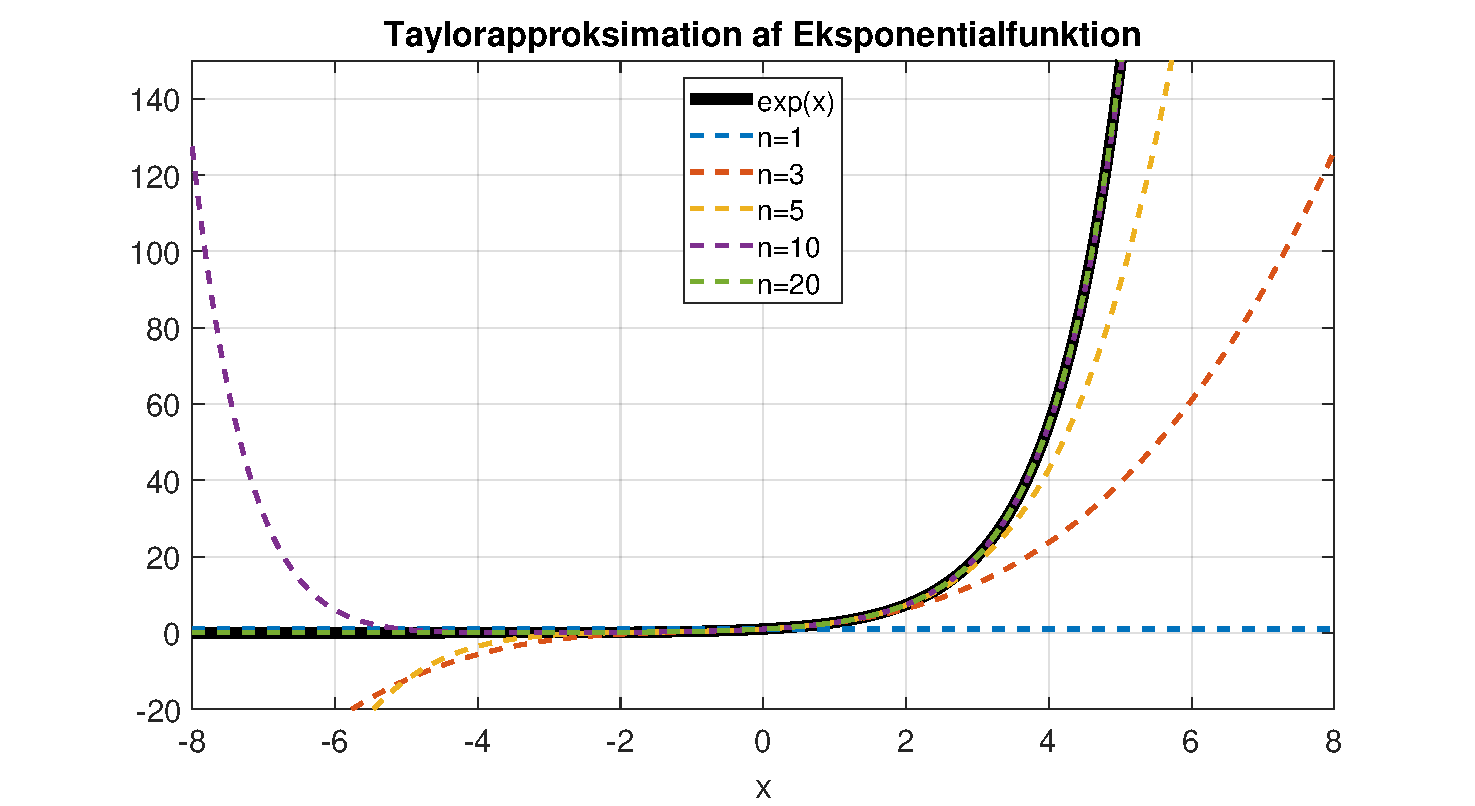
\includegraphics[scale=0.65]{matematik/Taylorseries_figure.pdf}
	\caption{Eksempel på hvordan en Taylorapproksimation af en funktion bliver mere og mere præcis jo flere led der tages med.}
	\label{Taylorseries_figure}
\end{figure}
Som en hjælp til opgaver har vi samlet Taylorrækkerne for nogle af de mest almindelige funktioner omkring $a = 0$ i tabel \ref{Taylorseries_table}.
\begin{table}[h!]
	\centering
	\caption{Taylorrækker for forskellige funktioner omkring punktet $a=0$.}
	\label{Taylorseries_table}
	\bgroup
	\def\arraystretch{2}
	\begin{tabular}{|c|c|c|c|}
		\hline
		\textbf{Funktioner}   & $e^x$ & $\cos(x)$ & $\sin(x)$  \\ 
		\hline
		\textbf{Taylorrækker} & $\sum\limits_{n = 0}^{\infty} \frac{(x-a)^n}{n!}$ & $\sum\limits_{n=0}^{\infty} (-1)^n \frac{x^{2n}}{(2n)!} $ & $\sum\limits_{n=0}^{\infty} (-1)^n \frac{x^{2n+1}}{(2n+1)!}$  \\ \hline
	\end{tabular}
	\egroup
\end{table}

\section{Komplekse Tal}

Formålet med dette afsnit er at give en kort introduktion til komplekse tal, da de er et vigtigt redskab i store dele af fysikken. Vi vil her ikke gå i dybden med den stringente matematiske konstruktion af de komplekse tal, men i stedet fokuserer på anvendelse og forskellige specifikke egenskaber, der er relevante for de ting, som I skal arbejde med på campen.\\

Før vi definerer, hvad komplekse tal er, vil vi først kigge på den imaginære enhed $i$, som er et meget vigtigt tal i forhold til at beskrive, hvad komplekse tal er. Den imaginære enhed er defineret som følger
\begin{eqnarray}
i^2 = -1 \ ,
\end{eqnarray}
og blev oprindeligt indført som løsningen til ligningen $x^2 = -1$, der ikke kan løses med reelle tal. Men med den imaginære enhed kan man løse denne type ligning på følgende måde
$$x^2 = -1 \quad \Rightarrow \quad x^2 = i^2 \quad \Rightarrow \quad x = \pm \sqrt{i^2} = \pm i \ .$$
Det virker måske lidt underligt, sådan at indføre et nyt tal som $i$ for at løse en ligning, men det skal understreges at tallet $i$ matematisk set er lige så rigtigt som de reelle tal. Nu hvor vi har indført den imaginære enhed, er vi nu klar til at give definitionen på et komplekst tal $z$. Definitionen lyder 
\begin{equation}
z = a+ib \ ,
\label{kompleks_def}
\end{equation}  
hvor $a$ og $b$ er reelle tal, der kaldes henholdsvis realdelen og imaginærdelen af det komplekse tal $z$\footnote{At $b$ kaldes imaginærdelen skyldes, at tal på formen $ib$, hvor $b$ er et reelt tal, kaldes for imaginære tal.}.  Dette skrives ofte som $\text{Re}(z) = a$ og $\text{Im}(z) = b$. Det næste spørgsmål vi skal kigge på er, hvordan man regner med komplekse tal. Mere specifikt skal vi starte med at kigge på addition, subtraktion, multiplikation og division, da disse regneoperationer dækker langt de fleste beregninger, som involverer komplekse tal. Lad derfor $z_1 = a+ib$ og $z_2 = c+id$ være to komplekse tal, og starte med at kigge på addition og subtraktion. Dette er defineret på den naturlige måde
\begin{align}
\label{kompleks_add}
z_1+z_2 = (a+c) + i(b+d) \ , \\
\label{kompleks_sub}
z_2-z_2 = (a-c) + i(b-d) \ .
\end{align}
Man lægger/trækker altså realdelene og imaginærdelene til/fra hinanden hver for sig. Når man skal gange komplekse tal sammen, gøres det ganske som man ville forvente. Man regner blot som om, man gangede to parenteser ud
$$z_1 z_2 = (a+bi)(c+id) = ac + iad + ibc + i^2bd = (ac-bd) + i(ad+bc) \ ,$$
hvilket giver os definitionen for multiplikation af komplekse tal
\begin{equation}
\label{kompleks_mul}
z_1z_2 = (ac-bd) +i(ad+bc) \ .
\end{equation}
Endeligt er der division, som kan defineres ud fra multiplikation. Dette kan illustreres ved følgende beregning
$$\frac{z_1}{z_2} = \frac{a+ib}{c+id} = \frac{a+ib}{c+id} \cdot \frac{c-id}{c-id} = \frac{(ac+bd) + i(bc-ad)}{c^2 + d^2} = \frac{ac+bd}{c^2 + d^2} + i \frac{bc-ad}{c^2 + d^2} \ ,$$
og definitionen for division af komplekse tal kan da skrives
\begin{equation}
\label{kompleks_div}
\frac{z_1}{z_2} = \frac{ac+bd}{c^2+d^2} + i\frac{bc-ad}{c^2+d^2} \ .
\end{equation}
Nu da de grundlæggende regneregler for komplekse tal er blevet gennemgået, vil vi gå videre og kigge på nogle af de andre vigtige definition og egenskaber ved de kompleks tal. Den første af disse er det der kaldes for den komplekst konjugerede af et komplekst tal $z$, og som skrives $z^*$. Hvis vi skriver $z = a+ib$ kan den komplekst konjugerede defineres som
\begin{equation}
z^* = a - ib \ .
\end{equation}
Man finder således den komplekst konjugerede af et komplekst tal $z$ ved blot at skifte fortegn på imaginærdelen. Den næste egenskab ved komplekse tal er det der kaldes for tallets modulus, og som skrives $\abs{z}$. Definitionen af modulus er da
\begin{equation}
\abs{z} = \sqrt{a^2 + b^2} \ ,
\end{equation}
og minder altså meget om definitionen for længden af en vektor i to dimensioner. Ud fra definitionen af modulus kan man også vise følgende praktiske regneregler
\begin{align}
\abs{z} &= \abs{z^*} \ , \\
\abs{z_1 z_2} &= \abs{z_1} \abs{z_2} \ , \\
\abs{z^n} &= \abs{z}^n
\end{align}
Dette bringer os videre til normkvadratet for komplekse tal\footnote{Grunden til at det kaldes for et normkvadrat er, modulus $|z|$ også i nogle sammenhænge kaldes for normen af $z$. Her holder vi os dog til at kaldes $|z|$ for modulus og $|z|^2$ for normkvadratet.}, der er defineret som følger
\begin{equation}
\abs{z}^2 = a^2 + b^2 \ .
\end{equation}
Der er altså som sådan ikke så meget nyt ved normkvadratet i forhold til modulus, men da normkvadratet optræder typisk i fysik, er det vigtigt at nævne alligevel. Specielt er følgende lighed god at kende
\begin{equation}
\abs{z}^2 = zz^* \ ,
\end{equation} 
og kan nemt eftervises ved en hurtig beregning. Det sidste vi skal kigge på nu her er Eulers formel, som er en af de mest brugbare relationer indenfor komplekse tal. Eulers formel siger at
\begin{equation}
e^{ix} = \cos(x) + i \sin(x) \ ,
\end{equation}
hvor $x$ er et reelt tal. Dette virker nok som en lidt underlig lighed, og det er umiddelbart også svært at se, hvad en eksponentialfunktion har at gøre med cosinus og sinus. En måde at bevise denne formel på er at skrive $e^{ix}$ som sin Taylorrække, og se at denne Taylorrække er lig med summen af Taylorrækken for cosinus plus $i$ gange Taylorrækken for sinus.

\section{Vektorer}
Den simpleste måde at beskrive en vektor på, er som noget der har både en længde og en retning. I forhold til notation er der forskellige måder at skrive vektorer på, f.eks. som et bogstav med en pil over $\vec{v}$. I fysikken er der dog tradition for at skrive vektorer med fed, altså $\v{v}$, så det gør vi også her. En god måde at illustrere vektorer på er vha. en pil, som det ses på Figur \ref{vektorfig}. Denne måde at beskrive en vektor på har den fordel, at man tydeligt kan se både længden og retningen af vektoren.
\begin{figure}[h!]
	\centering
	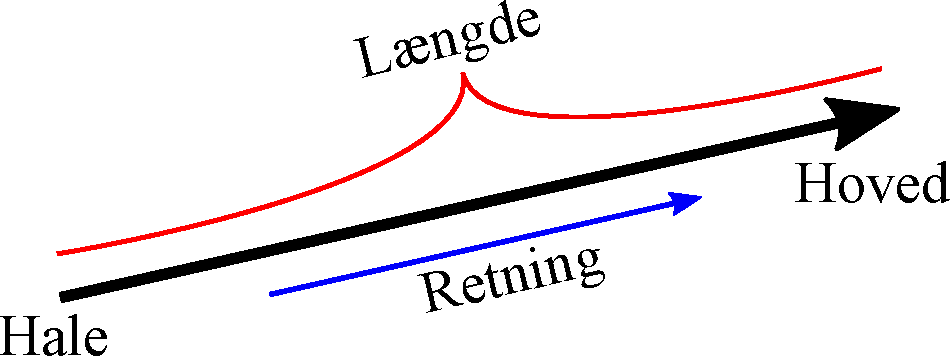
\includegraphics[scale=0.6]{matematik/fig/vektor.pdf}
	\caption{Den sorte pil er vektoren, og der er indikeret både vektorens længde og retning. }
	\label{vektorfig}
\end{figure}
Typisk vil man dog gerne regne med vektorer, og selvom det godt kan gøres vha. en grafisk metode, er der en anden repræsentation af vektorer, som egner sig bedre til dette. Denne kaldes for \emph{komposantform} (eller \emph{matrixform})  og tager udgangspunkt i et koordinatsystem. Da man i fysikken arbejder med den virkelige verden, som jo har tre rumlige dimensioner, vil vi i resten af afsnittet bruge et 3-dimensionalt koordinatsystem, som vist på Figur \ref{koordsys}. Specielt bruges et højrehåndet koordinatsystem, hvilket betyder, at hvis man tager højre hånd og peger sin tommelfinger i $x$-retningen og sin pegefinger i $y$-retningen, så vil langefingeren vise $z$-retningen, som det også ses på Figur \ref{koordsys}.\\
Ideen med komposantformen er, at man i et koordinatsystem kan beskrive en vektor, $\v{v}$, ved at angive tre tal $v_x,  v_y,  v_z$, som angiver, hvor meget vektoren peger i hhv. $x$-, $y$-, og $z$-retningen. Disse tal kaldes for vektorens komposanter, og man skriver vektoren:
\begin{equation}
\v{v} = \xyz{v_x}{v_y}{v_z}
\end{equation}
For at finde længden af vektoren, som man skriver $\abs{\v{v}}$, på komposantform, bruges Pythagoras sætning i tre dimensioner. Man får altså at:
\begin{equation}
\abs{\v{v}} = \sqrt{v_x^2 + v_y^2 + v_z^2}
\label{length}
\end{equation} 
Til sidst er det også vigtigt at vide, hvornår to vektorer er lig med hinanden. Det er de, hvis de har både samme længde og samme retning. På komposantform kan dette skrives:
\begin{equation}
\v{v} = \v{u} \quad \quad \text{hvis} \quad \quad
\begin{matrix}
v_x = u_x \\
v_y = u_y \\
v_z = u_z \\
\end{matrix}
\end{equation}
To vektorer er altså lig med hinanden, hvis deres komposanter er ens.
\begin{figure}[h!]
	\centering
	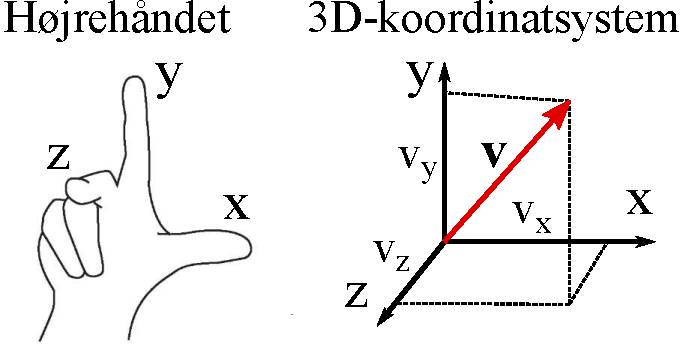
\includegraphics[scale=0.9]{matematik/fig/koordsys}
	\caption{På billedet til venstre ses reglen for et højrehåndet koordinatsystem. På billedet til højre er der vist et højrehåndet 3-dimensionalt koordinatsystem, og der er også indtegnet en vektor, $\v{v}$, med sine tre komposanter $v_x,  v_y,  v_z$.}
	\label{koordsys}
\end{figure}

\subsection{Regneregler for Vektorer}
I dette afsnit skal vi se på, hvordan man regner med vektorer. Det første spørgsmål som man kunne stille sig selv i denne forbindelse er, om man kan lægge/trække vektorer til/fra hinanden. Det kan man godt, og det gøres ved at lægge/trække komposanterne til/fra hinanden i par. Det skrives:
\begin{equation}
\v{v} \pm \v{u} = \xyz{v_x}{v_y}{v_z} \pm \xyz{u_x}{u_y}{u_z} = \xyz{v_x \pm u_x}{v_y \pm u_y}{v_z \pm u_z}
\end{equation}
En anden ting som man kan gøre med en vektor, er at gange den med en konstant $a$. Det gøres ved at gange tallet på hver af komposanterne, altså:
\begin{equation}
a \cdot \v{v} = a \cdot \xyz{v_x}{v_y}{v_z} = \xyz{a \cdot v_x}{a \cdot v_y}{a \cdot v_z}
\end{equation}
Det næste naturlige spørgsmål er nu, om man kan gange og dividere vektorer med hinanden. Det viser sig at division af vektorer ikke er defineret, men at der til gengæld er to forskellige måder at gange vektorer sammen på, som begge kaldes for vektorprodukter.\\

Den første er \emph{skalarproduktet} (eller \emph{prikproduktet}) og kaldes sådan, fordi resultatet er en skalar (altså et tal). Skalarproduktet af to vektorer skrives $\v{v} \cdot \v{u}$ og er defineret som:
\begin{equation}
\v{v} \cdot \v{u} = \xyz{v_x}{v_y}{v_z} \cdot \xyz{u_x}{u_y}{u_z}
= v_x \cdot u_x + v_y \cdot u_y + v_z \cdot u_z
\end{equation} 
Man tager altså vektorenes komposanter, ganger dem sammen i par og lægger det hele sammen. Specielt kan man kigge på skalarproduktet af en vektor med sig selv, og hvis man sammenligner med udtrykket for længden af en vektor, ligning \eqref{length}, ses, at $\v{v} \cdot \v{v} = \left| \v{v} \right|^2$. Det giver os en alternativ definition på længden af en vektor; $\abs{\v{v}} = \sqrt{\v{v} \cdot \v{v}}$.\\ 
Skalarproduktet har dog også en mere geometrisk definition, som tager udgangspunkt i vektorenes længde og vinklen mellem dem. Det er her vigtigt at understrege, at når man taler om vinklen mellem to vektorer, så menes der den mindste vinkel mellem dem, når man placerer halerne af vektorene oveni hinanden, som det ses på Figur \ref{dot_cross}. Med denne definition er skalarproduktet:
\begin{equation}
\v{v} \cdot \v{u} = \abs{\v{v}} \cdot \abs{\v{u}} \cdot \cos \theta
\end{equation} 
Det andet af de to vektorprodukter er \emph{krydsproduktet}, hvor resultatet er en ny vektor. Krydsproduktet skrives $\v{v} \times \v{u}$ og er defineret:
\begin{equation}
\v{v} \times \v{u} = \xyz{v_x}{v_y}{v_z} \times \xyz{u_x}{u_y}{u_z} = \xyz{v_y \cdot u_z - v_z \cdot u_y}{v_z \cdot u_x - v_x \cdot u_z}{v_x \cdot u_y - v_y \cdot u_x}
\end{equation} 
En vigtig egenskab ved krydsproduktet, som man ikke sådan lige kan se ud af definitionen er, at den resulterende vektor, $\v{c} = \v{v} \times \v{u}$, er vinkelret på både $\v{v}$ og på $\v{u}$. Kigger man igen på Figur \ref{dot_cross}, kan man da se, at der er to muligheder for, hvilken vej vektoren $\v{c}$ kan pege, så den er vinkelret på $\v{v}$ og $\v{u}$; nemlig ind i eller ud af figuren. Der er selvfølgelig kun en af disse, som er den rigtige retning, og heldigvis er der en nem huskeregel (typisk kaldet højrehåndsreglen) til at finde den rigtige. Man tager højre hånd og peger tommelfingeren i retningen af den første vektor og peger så sin pegefinger i retningen af den anden vektor. Da vil langefingeren give retningen af den nye vektor, $\v{c}$, på samme måde som den angiver $z$-retningen i et højrehåndet koordinatsystem. Tager man eksemplet på Figur \ref{dot_cross}, vil $\v{c}$ pege ind i figuren.\\
Ligesom med skalarproduktet har krydsproduktet også en mere geometrisk fortolkning. Det gælder nemlig at størrelsen af den vektor, som man får, når man laver et krydsprodukt, kan udtrykkes vha. længden af de to vektorer som man krydser med hinanden og vinklen mellem dem. Der gælder:
\begin{equation}
\abs{\v{v} \times \v{u}} = \abs{\v{v}} \cdot \abs{\v{u}} \cdot \sin \theta 
\end{equation}

\begin{figure}[h!]
	\centering
	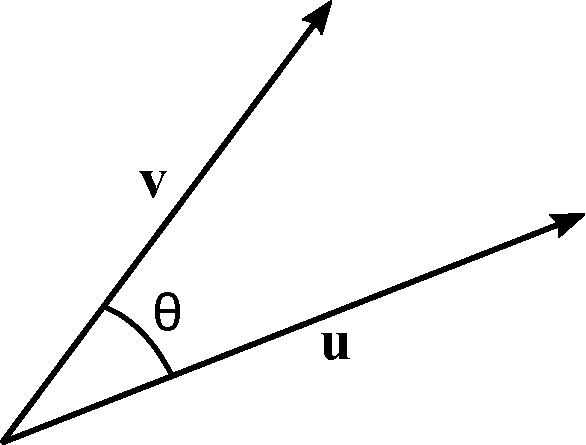
\includegraphics[scale=0.7]{matematik/fig/dot_cross.pdf}
	\caption{To vektorer og deres mellemliggende vinkel.}
	\label{dot_cross}
\end{figure}
Det sidste begreb er \emph{enhedsvektorer}, der er vektorer, som har en længde på 1. For at kunne kende forskel på en almindelig vektor og en enhedsvektor, bruger man en speciel notation, hvor man sætter en "hat" over vektoren, $\hatvec{v}$. Enhedsvektorer opfylder de samme regneregler som almindelige vektorer, og på den måde er der ikke meget nyt i dem. De er dog et vigtigt notationsmæssigt redskab og bruges i mange dele af fysikken. Specielt bruger man ofte enhedsvektorer, der peger langs en af de tre koordinatakser. Disse har en speciel notation og er skrevet op nedenfor:
\begin{equation}
\xhat = \xyz{1}{0}{0} \ , \quad \quad \yhat = \xyz{0}{1}{0} \ , \quad \quad \zhat = \xyz{0}{0}{1}
\end{equation}
Med disse tre enhedsvektorer kan man nu skrive enhver vektor, $\v{v}$, på følgende måde:
$$\v{v} = \xyz{v_x}{v_y}{v_z} = \xyz{v_x}{0}{0} + \xyz{0}{v_y}{0} + \xyz{0}{0}{v_z} = v_x \xhat + v_y \yhat + v_z \zhat$$
Denne metode, hvor man skriver en vektor som summen af flere andre vektorer, er vigtig at bide mærke i. Hvis en vektor, $\v{v}$, repræsenterer en fysisk størrelse, f.eks. en kraft, så vil den fysiske størrelse være uændret, om man skriver vektoren på den ene eller anden måde. Dette er praktisk, da man selv kan vælge på hvilken måde man skriver vektoren, alt efter hvilken fysisk problemstilling man prøver at løse. 
% \newpage
% \section{Opgaver}
%%
\subsection*{Differentialregning}
%%
\begin{opgave}{Hastighed og postion}
	\begin{figure}[h!]
		\centering
		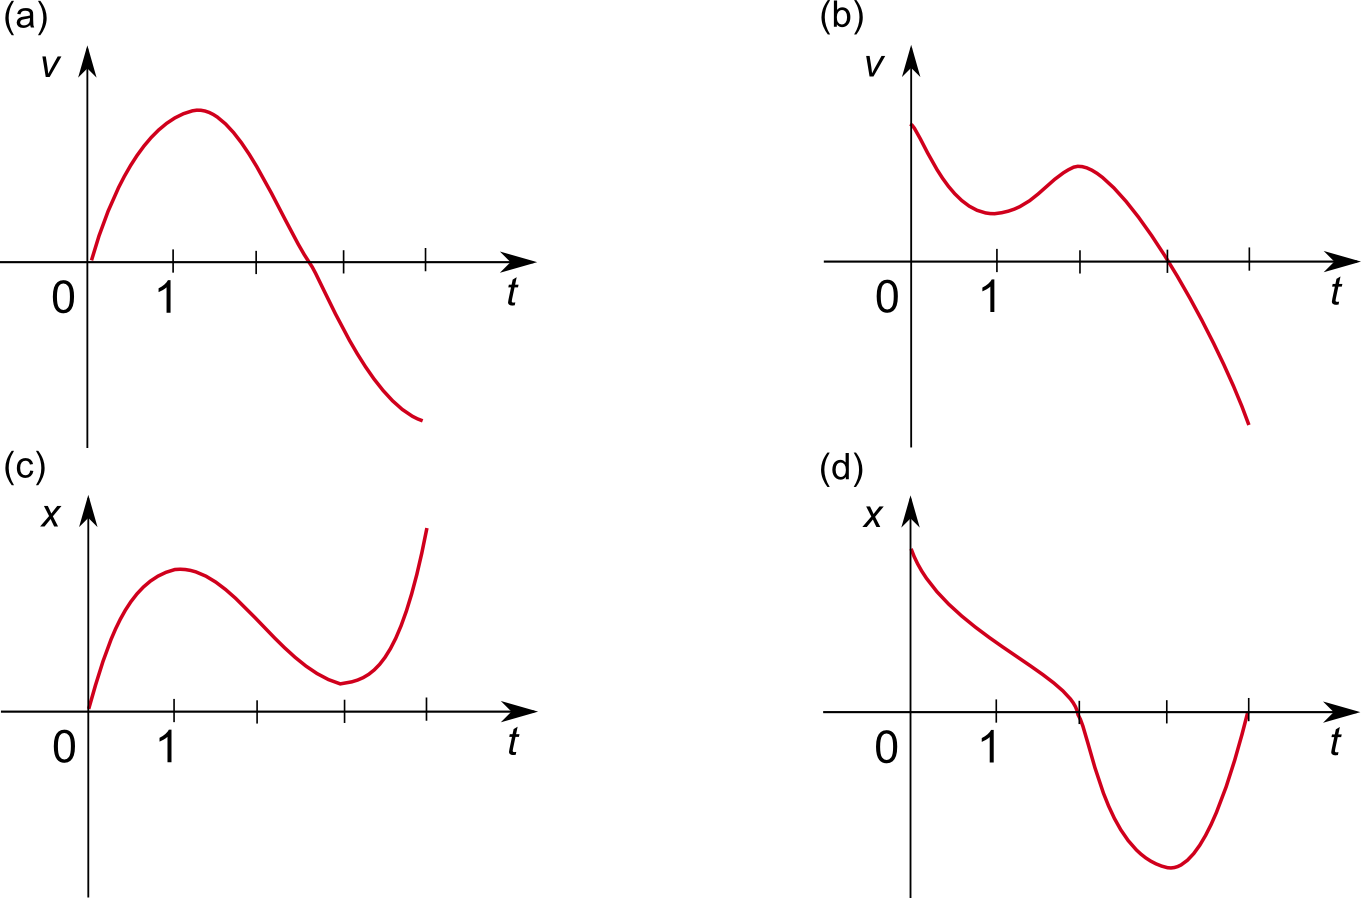
\includegraphics[width=0.47\textwidth]{opg/figurer/vx_grafer.png}
		\caption{Hastighed og position som funktion af tiden.}
		\label{fig:vx_grafer}
	\end{figure}
	\opg Figur \ref{fig:vx_grafer} (a) og (b) viser hastigheden af to objekter som funktion af tiden i sekunder. Hvornår sætter de to objekter hastigheden op, og hvornår sætter de hastigheden ned? Forklar dit svar.
	\opg Figur \ref{fig:vx_grafer} (c) og (d) viser positionen af to objekter $x$ som funktion af tiden i sekunder. Hvornår sætter de to objekter hastigheden op, og hvornår sætter de hastigheden ned? Forklar dit svar.
\end{opgave}
%%
%%
\begin{opgave}{Afledede og dobbeltafledede}
Find den afledede og dobbeltafledede med hensyn til $x$ for følgende funktioner:
\opg $f(x) = x^2 + 4x.$
\opg $f(x) = \frac{1}{x} + \frac{1}{x^2}.$
\opg $f(x) = \cos(x).$
\opg $f(x) = \ln(x).$
\opg $f(x) = x \sin(x).$
\opg $f(x) = \frac{1}{x} \ln(x).$
\end{opgave}
%%
%%
\begin{opgave}{Sammensatte funktioner}
Skriv følgende udtryk som en sammensat funktion $f(g(x))$ (altså skal du identificere den indre funktion $g(x)$ og den ydre funktion $f(g)$). Beregn derefter $\dv{f}{x}$.\\ 
\opg $f(x) = \sin (4x).$
\opg $f(x) = \sqrt{2x}.$
\opg $f(x) = \sqrt{4x+5}.$
\opg $f(x) = \sin(e^x).$
\opg $f(x) =  \ln \left( \cos x \right).$
\end{opgave}
%%
\subsection*{Integralregning}
%%
\begin{opgave}{Integraler og arealer under funktioner}
I matematikafsnittet i kompendiet nævnes det, at når man regner et bestemt integral
\begin{equation*}
\int^a_b{f(x)}\dd{x},
\end{equation*}
så svare det til arealet under grafen for $f(x)$ i intervallet $[a,b]$ på $x$-aksen. Brug dette faktum til at diskutere den fysiske forståelse af følgende udsagn.
\opg Hvis man integrerer en hastighed $v(t)$ ift. tiden $t$, så får man en position $x(t)$.
\opg Hvis man integrerer en acceleration $a(t)$ ift. tiden $t$, så får man en hastighed $v(t)$. \\
\end{opgave}
%%
%%
\begin{opgave}{Ubestemte integraler}
	Udregn det ubestemte integral af følgende funktioner:
	\opg $f(x) = x^3$.
	\opg $f(x) = x^2 + 4x$.
	\opg $f(x) = x^2 + \frac{1}{x^2}$.
	\opg $f(x) = \cos (x)$.
	\opg $f(x) = \frac{1}{x}$.
\end{opgave}
%%
\begin{opgave}{Størrelsen af en port}
    En tømmer er blevet hyret til at lave tre porte.
    Toppen af hver port kan beskrives med en af de følgende funktioner
    \begin{align*}
        f(x)&=1-x^2,\\
        g(x)&=2-\frac{e^x+e^{-x}}{2},\\
        h(x) &= 1-\abs{x}.        
    \end{align*}
    Alle portene er i intervallet $[-1/2,1/2]$.
    \opg Opstil bestemte integraler til at udregne arealet af de tre porte.
    \opg Hvilken port er størst?
    \opg Hvilken er mindst?
\end{opgave}
%%
\begin{opgave}{Ubestemte højereordensintegraler}
    Udregn følgende ubestemte højereordensintegraler. Sæt alle integrationskonstanter til nul.
    \opg $\iint ye^{-x}\dd{x}\dd{y}.$
    \opg $\iint y\cos(xy)\dd{x}\dd{y}.$
    \opg $\iiint (x^2+y^2)z\dd{x}z\dd{y}\dd{z}.$
    \opg $\iiint \sin(x)\sin(y)\sin(z)\dd{x}\dd{y}\dd{z}.$
\end{opgave}
%%
%%
%\begin{opgave}{Bestemte højere ordens integraler}
    %Udregn følgende bestemte højere ordens integraler
    %\opg $\int_0^1\int^0_{-\ln(2)} ye^{-x}\dd{x}\dd{y}$
    %\opg $\int_0^1\int_0^\pi y\cos(xy)\dd{x}\dd{y}$
    %\opg $\int_{-1}^1\int_{0}^{x}\int_{-1}^1 (x^2+y^2)z\dd{x}z\dd{y}\dd{z}$
    %\opg $\int_0^\pi\int_0^\pi\int_0^\pi \sin(x)\sin(y)\sin(z)\dd{x}\dd{y}\dd{z}$
%\end{opgave}
%%
%%
%\begin{opgave}{Lige og ulige funktioner} \label{opg:lige/ulige}
%En funktion, så som $f(x) = x^2$, der opfylder kravet, $f(x) = f(-x)$, kaldes en lige funktion. En funktion, som $f(x) = x$, der opfylder det lignende krav, $f(x)=-f(-x)$, kaldes for en ulige funktion.
%Det vil sige, at en lige funktion er uændret, hvis man spejler den i $y$-aksen, mens en ulige funktion skifter fortegn ved den samme spejling.
%Bemærk at de fleste funktioner er hverken lige eller ulige, og unikt er funktionen $f(x) = 0$ både lige og ulige.
%Afgør om følgende funktioner er lige eller ulige.
%\opg $\sin(x)$.
%\opg $e^{x^2}$.
%\opg $\cos(x)$.
%\end{opgave}
%%
%%
%\begin{opgave}{Integraler af lige og ulige funktioner.}
%Vi vil her finde nogle meget praktiske regneregler for integraler af lige og ulige funktioner, der er defineret i opgave \thechapter,\ref{opg:lige/ulige}, over et symmetrisk interval.
%Lad $f_l(x)$ være en lige funktion og $f_u(x)$ være en ulige funktion.
%Antag derudover at integralerne
%$$
%\int_0^a f_l(x)\dd{x}   \quad \text{og} \quad \int_0^a f_u(x)\dd{x}
%$$
%er kendte.
%\opg Vis at
%$$
%\int_{-a}^{a} f_l(x)\dd{x} = 2\int_0^a f_l(x) \, .
%$$
%\opg Vis at
%$$%\int_{-a}^{a} f_u(x)\dd{x} = 0 \, .
%$$
%\opg Brug dette til at løse integralet: $$\int_{-1}^1 {x^2\cos(x)\sin(x)+x^2-xe^{x^2}}\dd{x}$$
%\end{opgave}
%%
%%
%\begin{opgave}{Et spøjst integral}
    %Udregn
    %\opg $\int_0^{\pi} \cos(x)\dd{x}$
    %\opg $\int_\pi^{2\pi} \cos(x)\dd{x}$
    %\opg $\int_0^{2\pi} \cos(x)\dd{x}$
    %\opg $\int_0^{\pi/2} \cos(x)\dd{x}$
    %\opg $\int_{-8\pi}^{32\pi} \cos(x)\dd{x}$
    %\opg $\int_{-8\pi}^{32\pi} \cos[2019](x)\dd{x}$
    %\opg $\int_{-2019\pi}^{2019\pi} %\cos[2019](x)\dd{x}$
%\end{opgave}
%%
\subsection*{Differentialligninger}
%%
\begin{opgave}{Hvornår er det en løsning?}
	I denne opgave skal vi finde ud af, hvornår nogle forskellige funktioner er løsninger til de givne differentialligninger. Sagt med andre ord skal vi finde de specifikke talværdier for alle de konstanter, der indgår i funktionerne, således at funktionerne løser deres respektive differentialligningerne. Bemærk at der kan være mere end 1 værdi.
	\opg For hvilke værdier af $k$ løser funktionen
	\begin{align*}
	f(x) = \cos(kx)
	\end{align*}
	differentialligningen
	\begin{align*}
	4 \dv[2]{f(x)}{x} = - 25f(x) \, .
	\end{align*}
	\opg Tjek for de værdier af $k$ I fandt i 1), at funktionen $g(x) = A \sin (kx) + B \cos (kx)$ også løser differentialligningen
	\begin{align*}
	4 \dv[2]{g(x)}{x} = -25 g(x) \, .
	\end{align*}
	\opg For hvilke værdier af $r$ løser funktionen
	\begin{align*}
	h(x) = e^{rx}
	\end{align*}
	differentialligningen
	\begin{align*}
	2 \dv[2]{h(x)}{x} + \dv{h(x)}{x} - h(x) = 0 \, .
	\end{align*}
	\opg Lad $r_1$ og $r_2$ være de konstanter du fandt i \textbf{3)}. Tjek at funktionen $k (x) = ae^{r_1x} + be^{r_2x} $ også løser differentialligningen
	\begin{align*}
	2 \dv[2]{k(x)}{x} + \dv{k(x)}{x} - k(x) = 0 \, .
	\end{align*}
\end{opgave}
%%
%%
\begin{opgave}{Generelle 1. ordens differentialligninger}
I denne opgave skal du også vise, at nogle forskellige funktioner er løsninger til de givne differentialligninger. Denne gang er funktionerne og differentialligningerne dog skrevet op på en mere generel form, dvs. at de kan indeholde arbitrære konstanter.
\opg Vis at alle funktioner på formen
\begin{align*}
	h(x) = \frac{1}{x + A} 
\end{align*}
løser differentialligningen
\begin{align*}
	\dv{h}{x} = - h(x)^2 \; .
\end{align*}
\opg Vis at alle funktioner på formen
\begin{align*}
	k(x) = \left( c - x^2 \right)^{-1/2}
\end{align*}
løser differentialligningen
\begin{align*}
	\dv{k}{x} = x k(x)^3 \; .
\end{align*}
\opg Vis at alle funktioner på formen
\begin{align*}
	g(x) = \frac{\ln (x) + C}{x}
\end{align*}
løser differentialligningen
\begin{align*}
	x^2 \dv{g}{x} + xg(x) = 1 \; .
\end{align*} 
\opg Vis at alle funktioner på formen
\begin{align*}
	f(x) = \frac{1 + ce^x}{1-ce^x}
\end{align*}
løser differentialligningen
\begin{align*}
	\dv{f}{x} = \frac{1}{2} \left( f(x)^2 - 1 \right) \; .
\end{align*} 
\end{opgave}
%%
%%
%\begin{opgave}{Brugbare differentialligninger}
    %Bestem hvilken funktion f(t), der opfylder de følgende differentialligninger
   %\opg $\dv{f(t)}{t} = c \cdot f(t)$, hvor c er en arbitrær konstant, $c \neq 0$
   %\opg ${\dv{f(t)}{t}} = \frac{1}{2\cdot f(t)} $
   %\opg Vis at $f(t)=t^{2/3}$ er en løsning til differentialligningen 
   %$\dv{f(t)}{t} = \frac{2}{3\sqrt{f(t)}}$
%\end{opgave}
%%
%%
%\begin{opgave}{Dejlige andenordens differentialligninger, der er værd at kende}
    %Løs de følgende differentialligninger
    %\opg $\dv[2]{f(x)}{x}=0$
    %\opg $\dv[2]{g(x)}{x}=k$
    %\opg $\dv[2]{h(x)}{x} + h(x) = 0 $
    %\opg $\dv[2]{f(x)}{x} + \dv{f(x)}{x} = 0 $
    %\opg $\dv[2]{g(x)}{x} + \dv{g(x)}{x} = k $
    %\opg $\dv[2]{h(x)}{x} + \dv{h(x)}{x} + h(x) = 0 $
%\end{opgave}
%%
\subsection*{Logaritmer}
%%
\begin{opgave}{Logaritmeopgaver I}
    Find værdien af de følgende udtryk
    \opg $\log_{4}(8).$
    \opg $\log_{1/9}\left(\sqrt{27}\right).$
    \opg $\ln(e^{2/3}).$
    \opg $\ln(\frac{e^5}{e^3}).$
\end{opgave}
%%
%%
\begin{opgave}{Logaritmeopgaver II}
    Løs for den ukendte variabel
    \opg $\log_{b}(16) = 4/3.$
    \opg $\ln(x) = -1.$
    \opg $\log_{2}(1/x)=\frac{1}{5}.$
\end{opgave}
%%
%%
%\begin{opgave}{Logaritmeapproximationer}
%Brug approximationerne $\log_{10}(2) = 0,3010$ og $\log_{10}(3)= 0,4771$ til at udregne værdien af de følgende udtryk
    %\opg $\log_{10}(24)$
    %\opg $\log_{10}(5)$
    %\opg $\log_{10}(4^{\frac{1}{3}})$
%\end{opgave}
%%
%%
\begin{opgave}{En ekstra logaritmeregneregel}
    Ud fra de tre logaritmeregneregler, \eqref{mat:log}, vis at
    $$
    \frac{\log(a)}{b}=\log(a^{-b}).
    $$
\end{opgave}

\chapter{Kosmologi}
\section{Introduktion}
Kosmologi er læren om universets dannelse, udvikling og endeligt. Når der snakkes om universets størrelse, er det normalt det synlige univers, der menes. Dette er den del af universet, hvor lys er nået hen til os, så vi kan observere det. Længere ude er informationen ikke nået frem til os endnu, så vi ved ikke, hvor stort hele universet er. 

Det stemmer overens med \emph{det kosmologiske princip}, der siger, at universets love og konstanter er ens overalt og massen er ligeligt fordelt (set fra en stor nok skala). Det kan deles op i to postulater: Universet er homogent (ens i hvert område man vælger) og isotropt (ser ens ud, uanset hvilken retning man kigger i), som illustreret i figur \ref{isohomo}. Det kosmologiske princip behøver ikke gælde, men vi har ikke observeret noget, der bryder med det. Princippet antages derfor normalt at gælde, da det er det simpleste -- vi har ingen grund til at tro, at universets egenskaber pludselig ændrer sig et sted. Det er en god approksimation på skalaer fra \SI{200}{\mega\parsec} (megaparsec) og opefter. \SI{1}{\parsec} er cirka 3 lysår\footnote{Et lysår er den afstand lys tilbagelægger i løbet af et år og det har symbolet \si{\lightyear}.}, så et lysår er %$3\cdot 10^8$ lysår.
\SI{2.8e13}{\kilo\metre}. Således er $\SI{200}{\mega\parsec} \approx \SI{6e8}{\lightyear} \approx \SI{6e21}{\kilo\metre}$.
På små skalaer holder det selvfølgelig ikke. For eksempel er du tættere (har større massefylde) end luften omkring dig, og Solen kan udpege en særlig retning inden for solsystemet (den er speciel i forhold til planeterne, så en bevægelse ind mod den er speciel).

Antagelsen om, at universet er homogent og isotropt, er understøttet af
kortlægningen af den \emph{kosmiske mikrobølgebaggrund} (engelsk: CMB – cosmic microwave
background). Baggrunden består af stråling fra det tidspunkt, hvor universet blev
gennemsigtigt (ca. 380.000 år efter Big Bang, tror man) – altså hvor temperaturen af det plasma
og stråling som var dannet efter Big Bang er aftaget så tilstrækkeligt, at det var muligt for frie elektroner at 
kombinere med atomkerner og danne hydrogen og helium,
hvormed lys pludselig kunne bevæge sig næsten frit og derved undslippe. Af historiske årsager kaldes det \emph{rekombinationen}, da de første atomer dannes. At fotonerne derfor kunne bevæge sig frit kaldes \emph{fotonafkoblingen}, og disse to begivenheder skete næsten samtidig. Den kosmiske mikrobølgebaggrund er derfor det ældste
lys i universet! Dengang var strålingen i UV-området, men udvidelsen af Universet
(afsnit \ref{12}) har nu kølet baggrundsstrålingen til en temperatur på \SI{2.73}{\kelvin} eller \SI{-270.42}{\degreeCelsius} og flyttet den til mikrobølgeområdet (energi og temperatur er for stråling afhængige af hinanden). Den kosmiske mikrobølgebaggrund er blevet kortlagt af flere
missioner, først COBE (Cosmic Background Explorer), siden WMAP (Wilkinson
Microwave Anisotropy Probe) og senest \textit{Planck}, se figur \ref{CMB}. Det ses, at selv med høj opløsning er kortet uniformt – beviset på et næsten
homogent og isotropt tidligt univers. Men små fluktuationer i tætheden er stadig til
stede, og var det ikke for disse, ville den gravitationelle tiltrækning ikke have kunnet
ført til de galakser, vi observerer (og bor i!) i dag.

\begin{figure}[]
	\centering
	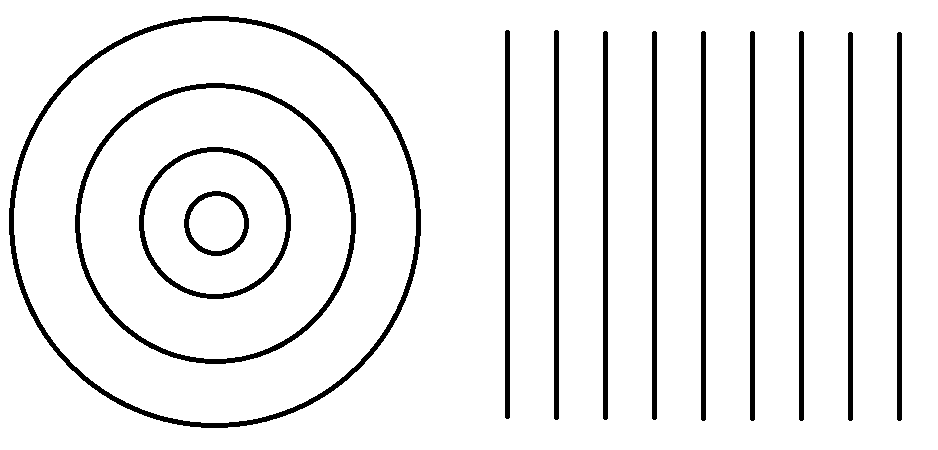
\includegraphics[width=0.7\textwidth]{Kosmo/2017/img/isohomo.png}
	\caption{Venstre: Illustration af isotropi. Fra midten ser verden ens ud i alle retninger. Højre: Illustration af homogenitet. Kigger man på et stort nok udsnit af verden, vil det se ud som alle andre udsnit.}
	\label{isohomo}
\end{figure}

\begin{figure}[]
	\centering
	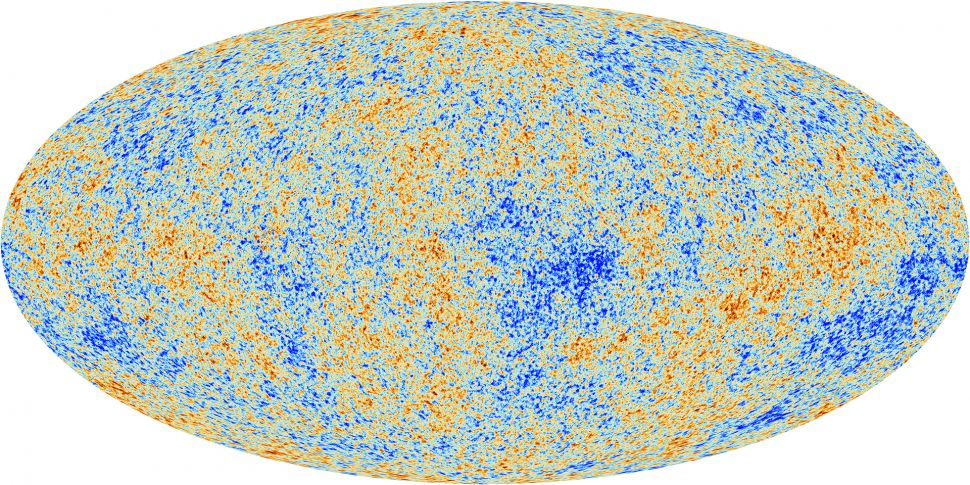
\includegraphics[width=0.7\textwidth]{Kosmo/2017/img/cmb_planck.jpg}
	\caption{Kortlægningen af den kosmiske mikrobølgebaggrund af COBE, WMAP og
		Planck. Mælkevejen, som ellers ville være til stede i billedet, er redigeret ud. Farverne viser de bittesmå temperaturfluktuationer på ± 300 µK. Kilde: \cite{CosmicMicrowaveBackgrounda}.}%\textit{Billedekilde: ESA og the Planck Collaboration}}
	\label{CMB}
\end{figure}
%Fra http:
%		//www.planetastronomy.com/astronews/astrn-2013/04/astron3.jpg

%\section{Big Bang og CMB}
\section{Rødforskydning}
\label{12}
\subsection{Dopplerforskydning}
Du kender nok til, at når en ambulance kører forbi, så lyder sirenens tone højere når den nærmer sig, og dybere når den kører væk. Det skyldes \emph{Dopplerforskydning}, %Find gerne lydklip til undervisningen
%Det skyldes, 
hvilket er at lydbølgerne skubbes sammen og strækkes, afhængigt af hvilken fart de udsendes med i forhold til lytteren. Hvis en ambulance kører mod dig, og du står stille, vil du høre bølgerne sammenpresset. Dette skyldes to ting: Først, så er lydens hastighed er uændret i mediet. Næst, så bliver lydbølgen udsendt under bevægelse, dvs. at i det tidsrum bølgen bliver sendt ud over, så flytter ambulancen sig også. Derfor vil bølgen virke til at have en kortere bølgelængde, da afstanden har ændret sig under udsendelse (se figur \ref{doppler}). %\\
Men hvis du selv kører med samme hastighed foran ambulancen, så vil du høre dem på samme måde, som de bliver udsendt - altså på samme måde som hvis begge biler står stille, da det er den relative hastighed, som er afgørende.

\begin{figure}[h!]
	\centering
	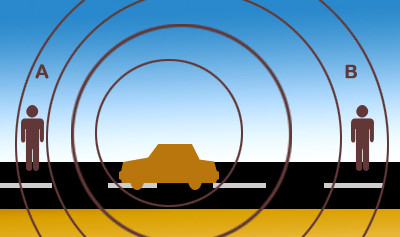
\includegraphics[width=0.7\textwidth]{Kosmo/2017/img/doppler.jpg}
	\caption{Dopplerforskydning af lyden fra en bil, der kører mod venstre. Person A vil høre end højere tone end person B, og personen i bilen vil høre noget et sted derimellem. Ringene viser et fast punkt på lydbølgerne. Kilde: \cite{DopplerIllustration}.}
	\label{doppler} 
\end{figure}

Det samme sker for lys. Hvis en ambulance kører væk, vil både tonen af sirenen blive dybere og lyset fra lygterne en smule rødere. Med rødere menes her, at lyset forskydes til at få en længere bølgelængde, og da rødt lys er den del af det visuelle spektrum der har længst bølgelængder, så vil visuelt lys se rødere ud. Man kalder det derfor også rødforskydning generelt. \\
Bemærk dog, at selvom fotoner og lydbølger har højere energi ved korte bølgelængder, så mister de ikke energi ved Dopplerforskydning - der er bare sket et skift i perspektivet, man ser bølgerne fra. Fra bølgens eget synspunkt (hvis man følger den) har den samme bølgelængde og energi hele tiden.
\subsection{Kosmologisk Rødforskydning}
Edwin Hubble er en kendt skikkelse, som i 1920'erne var involveret i opdagelsen, at galakser langt borte ser rødforskudte ud, men dette skyldes \emph{ikke} Dopplerforskydning fra galaksernes egenhastighed\footnote{Egenhastighed vil sige den hastighed som galaksen ''selv'' oplever at den har.} i forhold til os. Så ville vi have forventet, at lige så mange galakser var rødforskudte som blåforskudte, hvis de starter med en tilfældig hastighed. Og det gør de jo -- for hvorfor skulle de alle have en særlig retning i forhold til os? Det ville bryde med isotropien. 

Hubble bemærkede, at galakserne oftere er rødforskudt end blåforskudt, ja næsten altid rødforskydte, og jo længere væk de er, desto mere rødforskudte er de også. Georges Lemaître havde dog allerede formuleret og observeret, hvad der nu kaldes \emph{Hubble–Lemaîtres lov} (tidligere kendt som Hubbles lov), der beskriver den direkte proportionalitet mellem afstand og fart af en galakse (hvortil Hubble bidrog med mere data):
\begin{align}
v=H_0 D, \label{Hubbleslaw}
\end{align}
hvor $v$ er farten væk fra os, $D$ er afstanden til galaksen, og $H_0$ er Hubbles konstant, som er den nuværende værdi af Hubbleparameteren (der ikke er konstant, men ændrer sig meget langsomt). Det er desværre vanskeligt at sige præcis hvad værdien af Hubblekonstanten er, da forskellige typer datasæt, giver forskellige resulater. Dette er naturligvis interessant, og et af de mysterier astrofysikere lige nu arbejder på at løse. Værdien lader i hvert fald til at ligge omkring $\SI{70}{\kilo\meter\per\second\per\mega\parsec}$ - et af budene er $H_0 = \SI{67.7\pm0.5}{\kilo\meter\per\second\per\mega\parsec}$\cite{planck}.

Galaksers relative hastighed til os er altså større, desto længere væk de er. Og sådan vil det se ud fra ethvert punkt i universet. Derfor må rødforskydningen stamme fra, at alting bevæger sig længere væk fra hinanden, som rosiner i en hævende bolle. Det er netop, hvad der sker -- universets `dej' dvs. selve rumtiden\footnote{Begrebet rumtid kommer af at man i relativitetsteori betragter rum og tid som værende to sider af samme sag. Man siger at verden eksisterer i tre rummelige og en tidslig dimension, hvor de fire dimensioner tilsammen udgør rumtiden.} `hæver'. Galakserne har lige ofte egenhastigheder, der går mod os, som væk fra os, men hastigheden, som selve rumtiden udvider sig med, er vigtigere for galakser langt væk, fordi der er så meget rum imellem dem og os. For fjerne galakser skal lyset bevæge sig gennem mere rum for at nå frem til os. Derfor når lyset at blive strukket mere end ved nære galakser, da rummet når at udvide sig mere under lysets rejse, og bølgelængden således når at blive strukket mere.

Ved rødforskydning fra universets udvidelse mister lyset rent faktisk energi i modsætning til almindelig Dopplerforskydning. Dette er selvfølgelig et brud på energibevarelse, men det er egentlig ikke et problem, da man ikke kan betragte universet som et lukket system, fordi det udvider sig. Energibevarelse behøver kun at gælde i lukkede systemer. Nogle mener dog, at ændringen i energi fra universets udvidelse (og den mørke energi der opstår, se afsnit \ref{bestanddele}) udlignes af, at den gravitationelle energi falder til endnu lavere negative niveauer, således at universets totale energi altid er 0.

Måden, man måler rødforskydningen på, er ved at opsplitte lyset i dets forskellige bølgelængder. Dvs. man tager spektre af fjerne objekter, og derefter genkender man mønstre fra laboratorier på Jorden. Niels Bohr fik ideen, at elektroner kun kan eksistere i bestemte baner om en atomkerne, men ikke mellem disse. Hver bane har en bestemt energi, så elektronernes energi i atomer er kvantiseret, dvs. de kan kun have den energi, der svarer til lige præcis banernes energier. %findes kun i bestemte pakker. 
Når en elektron henfalder til en lavere tilstand, kommer den af med overskydende energi ved at udsende en foton -- en lyspartikel. Hvis en foton med passende energi rammer en elektron, kan fotonen blive absorberet, så elektronen kommer op i en højere energitilstand. 

For lysspektrer gælder 3 love, kaldet Kirchoffs love (ikke at forveksle med Kirchoffs love for elektriske kredsløb), som er illustreret i figur \ref{kirchoff}.
\begin{itemize}
	\item Varme, uigennemsigtige objekter udsender lys kontinuert over hele spektret. Ideelt set ville det give spektret for sortlegemestråling og det er en særligt god approksimation for varme stjerner. Sortlegemestråling er almindelig stråling som følge af, at objektet er varmt, hvilket beskrives ved en lyskurve, under navnet Planckkurven, som er afhængig af overfladetemperaturen af objektet. Mindre stjernes lys er mere `forurenet' af effekter fra molekylær hydrogen, der er relativt koldt, og andre stoffer.
	\item Varme, gennemsigte gasser udsender lys (da elektroner exciteres og henfalder) og danner emissionsspektra.
	\item Kolde gasser danner absorptionslinjer. Hvis en stjerne ligger bagved og sender lys mod os, vil skyen absorbere lyset og udsende det senere i en tilfældig retning. Dette betyder i længden, at det vil sende lys ud jævnt i alle retninger, hvilket giver en kraftig reduktion i mængden af lys der når os, da alt lyset pludselig skal fordeles i alle retninger. Så derfor ser vi mindre lys ved denne bølgelængde, end hvis gassen ikke havde været der.
\end{itemize}

\begin{figure}[h]
	\centering
	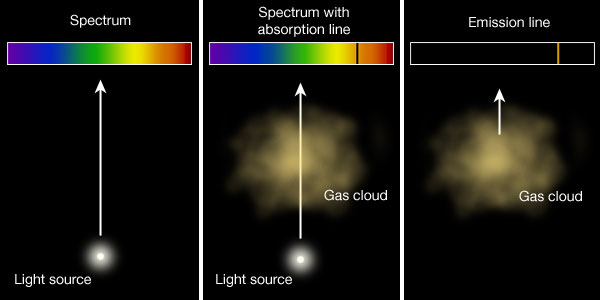
\includegraphics[width=0.6\textwidth]{Kosmo/2017/img/kirchoffslaws.jpg}
	\caption{Kontinuert spektrum (til venstre), absorptions-spektrum (midtfor) og
		emissions-spektrum (til højre). Kilde: \cite{AbsorptionEmissionSpectra}.}
	\label{kirchoff}
\end{figure}
%fra http://astro.psu.edu/public-outreach/fireworks-masks-1/absorption-and-emission-spectra

\begin{figure}[h!]
	\centering
	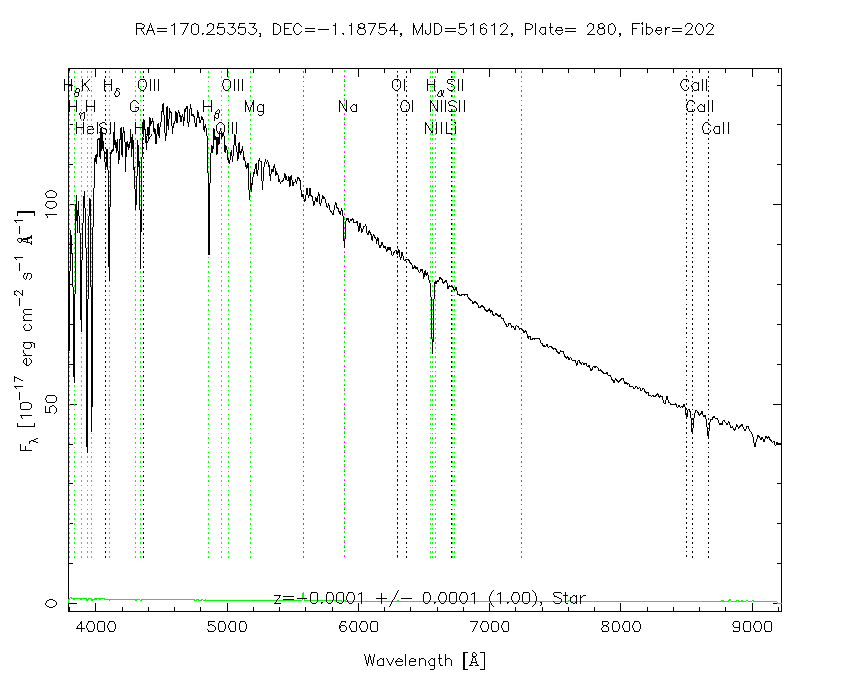
\includegraphics[width=0.6\textwidth]{Kosmo/2017/img/spektrum.png}
	\caption{Et typisk stjernespektrum. Y-aksen skal forstås som intensitet, mens der
		på X-aksen er bølgelængde i ångstrøm (Å) (1 Å = $10^{-10}$ m). Dykkene i intensitet
		er angivet med en overgang tilhørende et grundstof, som er identificeret i stjernens
		atmosfære. Kilde: \cite{Stjernespektrum}.}
	\label{spektrum}
\end{figure}
%fra http://i.stack.imgur.com/RMHmB.gif

Har man en galakse med en stjerne, som udsender et bredt spektrum af lys, vil lyset både bevæge sig gennem stjernens ydre `kolde' lag og galaksens gasskyer, før det når os. Stjerner og skyer består af forskellige stoffer såsom hydrogen. Når de belyses, absorberer hydrogenet fotoner med de energier, der svarer til energiforskellen mellem banerne i hydrogen. Der dannes derfor et helt bestemt mønster af absorbtionslinjer i spektret, som er unikt for i dette tilfælde hydrogen. For en rødforskudt galakse vil mønsteret ligge ved længere bølgelængder, end det vi måler for hydrogen på Jorden, men det er stadig genkendeligt, som det samme mønster. Et eksempel er vist i figur \ref{spektrum}. Når vi kan genkende et mønster af absorptionsliner eller emissionslinjer, selvom det ligger forskudt ved andre bølgelængder end normalt, så kan vi finde rødforskydningen. Den er defineret som forskellen mellem den observeret bølgelængde $\lambda_\text{obs}$ og den i laboratoriet målte bølgelængde $\lambda_\text{lab}$ i forhold til laboratoriebølgelængden (se figur \ref{redshiftmeasure}). Det er altså den relative forskydning i forhold til den oprindelige bølge. Lad os opskrive det som
%
\begin{align}
z=\frac{\lambda_\text{obs}-\lambda_\text{lab}}{\lambda_\text{lab}}. \label{redshifty}
\end{align}
%
\begin{figure}
	\centering
	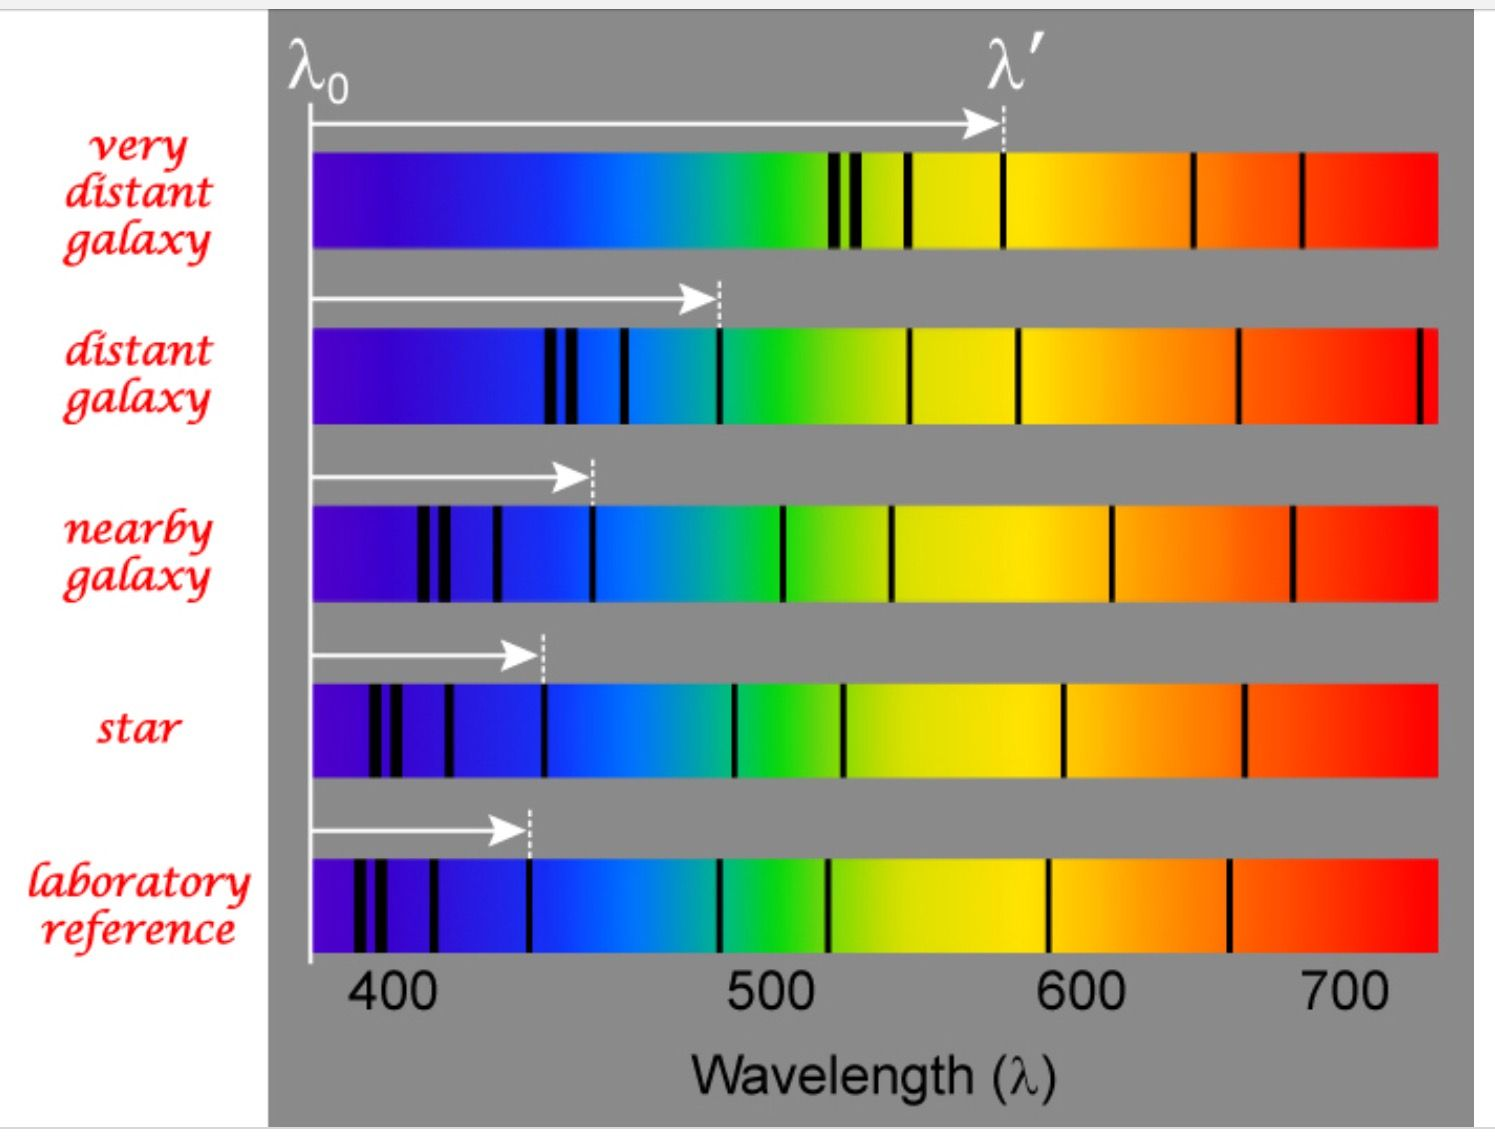
\includegraphics[width=0.6\textwidth]{Kosmo/2017/img/redshiftcomparison.jpg}
	\caption{Ligning \eqref{redshifty} bruges ved at måle de indbyrdes forhold mellem absorptionslinjerne i de forskellige spektra. Kilde: \cite{SNC1DEarthSpace}.}
	\label{redshiftmeasure}
\end{figure}
%
Rødforskydningen, $z$, er relateret til farten, $v$, således:
\begin{align}
z+1=\sqrt{\frac{1+\frac{v}{c}}{1-\frac{v}{c}}}.
\end{align}
For hastigheder meget langsommere end lysets hastighed i vakuum, $v \ll c$, kan det forsimples til:
\begin{align}
z\approx\frac{v}{c}.
\end{align}
%
Rødforskydning er altså en form for afstandsmål (da farten, $v$, hænger sammen med afstanden, $D$, ifølge ligning~\eqref{Hubbleslaw}), men også et tidsmål, da lyset har rejst i lang tid, hvis det har nået at passere en stor afstand og er blevet meget strukket. Hvordan rødforskydningen relaterer til andre måder at måle afstand på, afhænger af hvordan rumtiden strækker lyset. Det kan afgøres af universets form via generel relativitetsteori.

\section{Universets Form}

Universet har samlet set en form. Vi har 3 tydelige rummelige dimensioner omkring os, og vi er vant til, at hvis man tegner to parallelle linjer, så vil de aldrig krydse, og en trekant har altid en vinkelsum på \SI{180}{\degree}. Dette gælder dog kun i fladt rum! Forestil dig f.eks. en trekant tegnet på en globus; den vil faktisk have en vinkelsum på mere end \SI{180}{\degree}. På samme måde vil en trekant tegnet på en saddel have en vinkelsum, der er mindre end \SI{180}{\degree}, som på figur \ref{shapes}. Hvis universet er kugleformet, siges det geometrisk at have en positiv krumning, og hvis det er saddelformet (hyperbolsk), siges det geometrisk at have en negativ krumning. I et fladt univers er krumningen 0.

\begin{figure}[h!]
	\centering
	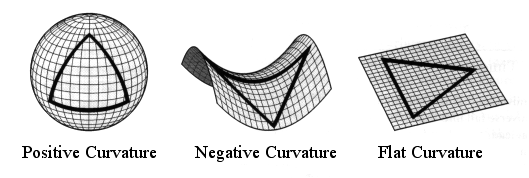
\includegraphics[width=0.7\textwidth]{Kosmo/2017/img/universe_geometry.png}
	\caption{Trekanter i forskellige geometrier har forskellige vinkelsummer. Kilde: \cite{GeometryUniverse}.}
	\label{shapes}
\end{figure}

Hvis et objekt er i frit fald, eller hvis man har en lysstråle, vil de bevæge sig langs en ret linje i rumtiden (kaldet en geodæt). Men hvis selve rumtiden krummer, så gør den `rette' linje det også. Derfor kan man se universets krumning ved at kigge på lyset fra objekter langt væk. Den viser sig ved, om ting ser forstørrede eller formindskede ud (om strålerne spredes eller samles som i en linse). Disse målinger viser, at universet er fladt med en præcision på \SI{0.5}{\percent}. Det vender vi tilbage til i afsnit \ref{bestanddele}. %Kilde + illustration

Hvis universet var positivt krumt og småt nok, ville det også betyde, at lyset kunne nå hele vejen rundt, og vi ville se de samme objekter flere steder på himlen, hvilket heller ikke er observeret. Til dette, forestil dig at du kaster en bold hårdt nok til, at den rammer dig i nakken igen. Så det synlige univers er i hvert fald meget fladt -- men måske har rumtiden en svag krumning, der bare ikke kan ses her. Selvom Danmark ser fladt ud, kan hele jordkloden jo godt være rund.

Hvis universet er positivt krumt, er det endeligt, mens fladt eller negativt krumt rum kan være uendeligt stort. Det er dog også muligt for universet både at være f.eks. fladt og endeligt, men så bryder man det kosmologiske princip.

Vi kan sammenligne universets størrelse ved forskellige tidspunkter gennem en skalafaktor $a(t)$. Vi definerer den nuværende faktor til 1, dvs. $a(t_\text{0})=1$, hvor $t_0$ er tiden nu. Der gælder:
\begin{align}
\frac{a(t_0)}{a(t)}=1+z, \\
a(t)=\frac{1}{1+z}.
\end{align}
Så man kan let omregne rødforskydning til skalafaktoren, fra dengang lyset blev udsendt.
%
Som beskrevet % i \ref{Hubble}
i forbindelse med ligning \eqref{Hubbleslaw} er Hubblekonstanten ikke konstant, men blot den nuværende værdi af Hubbleparameteren. Hubbleparameteren er faktisk
\begin{align}
H=\frac{v}{D}=\frac{\dot{a}}{a},
\end{align}
hvor $\dot{a} = \dd{a}/\dd{t}$, altså skalafaktoren differentiereret mht. tiden, eller den relative ændring i skalafaktoren. Hvis vi sætter det i anden og bruger noget generel relativitetsteori, som desværre er lidt for langhåret til at vi her vil vise det, får vi \emph{Friedmannligningen},
\begin{align}
H^2=\left(\frac{\dot{a}}{a}\right)^2=\frac{8\pi G \rho}{3}-\frac{\kappa c^2}{a^2}+\frac{\Lambda}{3}, \label{friedmann}
\end{align}
hvor $\rho$ er densitet. Hvis universet er fladt, må det have en helt bestemt samlet densitet kaldet den kritiske densitet $\rho_\text{c} = \SI{8.6e-27}{\kilo\gram\per\cubic\metre}$. Friedmannligningen er super interessant, da den viser os, hvordan universet udvikler sig. Det er en andenordensdifferentialligning med $a$ indeholdende konstanter som gravitationskonstanten, $G$, og lysets fart i vakuum, $c$. $\kappa$ kan være 1, 0 og -1 og dette afgør krumningen, der som bekendt kan være positiv, 0 eller negativ. $\Lambda$ er den kosmologiske kontant. Uden denne ville rumtiden trække sig sammen, fordi massen krummer det, så Einstein introducerede $\Lambda$ for at holde universet statisk. Det har han senere kaldt sin største fejl, efter Hubble opdagede, at universet er dynamisk. Man har dog genintroduceret konstanten for at accelerere udvidelsen, da man opdagede universets acceleration i 1998. Grunden til denne acceleration er blevet tolkende som værende en form for energi, kaldet \emph{mørk energi}. Lad os se på, hvad det egentlig er.

\section{Universets Komponenter} \label{bestanddele}
Universets udvikling og skæbne afhænger af dets indhold. Det består af:
%
\begin{itemize}
	\item Stråling/relativistisk stof: Fotoner og neutrinoer\footnote{Se kapitel \ref{chap:Partikelfysik} om partikelfysik for en grundig gennemgang af disse partikler.\label{note:partikel}}, fordi de har ingen eller meget lav masse samt høj hastighed, hvilket betyder at deres energi vil være domineret af kinetisk/relativistisk energi, og ikke deres masse (her menes hvilemasse)).
	\item Stof: Almindeligt stof, antistof og mørkt stof har alle masse, så her kalder vi dem samlet set `stof'. Egenskaben masse afgør, hvor stor en krafter man skal bruge på at accelerere partiklerne, men også hvor meget de krummer rumtiden omkring sig. Stof kan også betegnes som `ikke-relativistisk' stof, dvs. stof der er domineret af masse, og ikke kinetisk energi. Det stof, der ikke er mørkt stof, kalder man nogle gange \textit{baryonisk}, da det mest består af baryoner\footref{note:partikel}. Baryoner er partikler med et ulige antal kvarker\footref{note:partikel}, fx protoner (up, up, down) og neutroner (up, down, down).
	\item Kosmologisk konstant: Den form for mørk energi (nogle kalder det også vakuumenergi), vi antager universet er fyldt med. Det får universets udvidelse til at accelerere, er ligeligt fordelt overalt og fortyndes ikke fra udvidelsen. Det vides ikke om dette er en enkelt, samlet ting, eller en gruppe af ting (ligesom de ovenstående).
\end{itemize}
%
Disse komponenter påvirker universets form og udvikling forskelligt. Mængden af stof er nogenlunde konstant, men universet udvider sig i alle 3 rummelige dimensioner, så massedensiteten falder med:
\begin{align}
\rho_\text{m} \propto a^{-3}.
\end{align}
Stråling har næsten ingen \emph{hvilemasse}, hvilket er den masse et objekt har når den står stille, men ved høj fart får de, hvad man kalder en relativistisk masse. Fotoner har jo energi,$E$, og impuls,$p$, og ifølge Einsteins ligning $E^2=(mc^2)^2 + (pc)^2$ kan disse konverteres til masse,$m$, og derved interagerer dermed stadig via tyngdekraften og dermed rumtiden. Det er derfor lys ikke kan undslippe sorte hullers masse, selvom lyset ikke har en hvilemasse. Denne `effektive masse' bøjer rummet omkring sig, så stråling får universet til at trække sig sammen, ligesom stof. Stråling har dog den ekstra egenskab at det rødforskydes. Derfor fortyndes energien af stråling både med universets udvidelse, $a^{-3}$, og en ekstra faktor fra rødforskydningen, $a^{-1}$, fordi lys mister energi når dets bølgelængde bliver større. Strålingstætheden skalerer således med skalafaktoren som
\begin{align}
\rho_\text{R}\propto a^{-4}.
\end{align}

Mørk energi ved man ikke særlig meget om, men man formoder ofte, det stammer fra energien i vakuum. Der er dog et ekstremt stort problem ved dette -- et bud på vakuumenergidensiteten fra kvantefeltteori\footnote{Kvantefeltteori er den bedste beskrivelse man har af universets mindste bestanddele og bruges derfor i partikelfysik. I alle andre sammenhænge fungerer den rigtig godt, hvorfor dens bud på vakuumdensiteten er værd at bemærke. At kvantefeltteori giver en så forkert forudsigelse illustrerer et af de største uløste problemer i fysik: Foreningen af kvantemekanik og generel relativitetsteori.} er $10^{124}$ gange større end universets kritiske energidensitet, $\rho_\text{c}$ (se %\textit{Introduction to cosmology} af Barbara Ryden 
\cite{rydenIntroductionCosmology2006})!  Det lader altså til den mest sandsynlige mængde energi i vakuum er alt for stor i forhold til vores observationer. Dette kan ses som et af mange usandsynlige tilfælde, der gør, at universet akkurat passer til, at liv kan opstå. Denne problemstilling er kendt som \emph{the finetuning problem}, og der er mange mulige løsninger på det. De er ofte ganske farverige, f.eks. multiverser, virtuelle universer og brud på det kosmologiske princip gennem variende konstanter på tværs af sted. %\cite{TheAccUniverse} 

I den simple antagelse, at mørk energi består af en ''kosmologisk konstant'', vil energien ikke fortyndes, så der hele tiden opstår mere mørk energi med udvidelsen og densiteten er konstant.
\begin{align}
\rho_\Lambda = \text{konstant}
\end{align}

Lad os definere en densitetsparameter $\Omega$, som densitet i forhold til den kritiske densitet $\rho_\text{c}$ (som beskrevet i afsnit \ref{bestanddele}):
\begin{align}
\Omega=\frac{\rho}{\rho_\text{c}}.
\end{align}
Hvis vi indsætter densiteten af hver parameter får vi
\begin{align}
\Omega_{\text{m},0}=0.3089\pm 0.0062 \quad , \quad
\Omega_{\text{R},0}&=8.24\cdot 10^{-5} \quad , \quad
\Omega_{\Lambda,0}=0.6911\pm 0.0062, \\
\Omega_{\text{total},0}=\Omega_{m,0} + &\Omega_{R,0} + \Omega_{\Lambda,0}=1.000\pm0.005 \label{Omegatot} \cite{planck}
\end{align}
%
0 er i subscript for at vise, at det er nuværende værdier, ligesom $H_0$ er den nuværende værdi af Hubbleparameteren, $H$. Den samlede densitet er altså lig med eller meget tæt på den kritiske densitet, så det synlige univers lader til at være fladt. Som nævnt indeholder ''stof''  både synligt, baryonisk stof (dvs. velkendt stof som neutroner, protoner og lignende) og mystisk mørkt stof. Tætheden af stof kan således opdeles således:
\begin{align}
\Omega_{\text{B},0}=0.049\pm 0.001 \quad , \quad
\Omega_{\text{DM},0}=0.259\pm 0.006, \cite{planck}
\end{align}
hvor $\Omega_\text{B}$ og $\Omega_\text{DM}$ er densitetsparameteren for henholdsvis baryonisk stof og mørkt stof (engelsk: \textit{Dark Matter}). Det stof, vi omgiver os med til hverdag, udgør altså blot \SI{5}{\%} af universets indhold, mens \SI{26}{\%} er mørkt stof, som vi ikke ved meget om, og \SI{69}{\%} er mørk energi, som vi ved næsten intet om. Og det hele går lige op, så den samlede densitet giver et univers, der ser fladt ud, indenfor de usikkerheder vi arbejder med. Mørkt stof er beskrevet nærmere i afsnit \ref{DM}. Det er værd at bemærke at alt dette er observationelle resultater, og det er ganske bemærkelsesværdigt at vi ender med at have en densitet så nær den kritiske densitet.

Alt dette gør os i stand til at skrive Friedmannligningen på en lidt lettere og mere overskuelig form, nemlig som funktion af de forskellige densiteter og skalafaktoren. Den bliver således:
\begin{align}
\frac{H^2}{H_0^2}=\Omega_{\text{R},0}\cdot a^{-4} + \Omega_{\text{m},0}\cdot a^{-3} + \Omega_{\Lambda,0} \label{friedmann_component}
\end{align}
Denne ligning kan også skrives som:
\begin{align}
    \frac{\dot{a}^2}{a^2} &= H_0^2\left(\Omega_{\text{R},0}\cdot a^{-4} + \Omega_{\text{m},0}\cdot a^{-3} + \Omega_{\Lambda,0}\right) \\
    \Leftrightarrow \dot{a}^2 &= H_0^2 \left(\Omega_{\text{R},0}\cdot a^{-2} + \Omega_{\text{m},0}\cdot a^{-1} + \Omega_{\Lambda,0} \cdot a^2\right).
\end{align}
Af ligning \eqref{friedmann_component} kan det da udledes hvornår de forskellige komponenter har betydet mest for universets udvikling, noget vi nu vil dykke meget mere ned i.

\subsection{Komponenternes Udvikling}
Hver komponent i universet har en faktor, $\omega$, som afgør hvor stort tryk, $p$, de yder, hvilket er beskrevet ved \emph{tilstandsligningen},
\begin{align}
p=\omega \rho.
\end{align}
Vi kan desuden beskrive densiteten af hver komponent som
\begin{align} \label{density}
\rho = \rho_0 a^{-3(1+\omega)} = \frac{\rho_0}{a^{3(1+\omega)}}.
\end{align}
For stråling er $\omega = 1/3$, for stof er $\omega=0$ og for den kosmologiske konstant er $\omega=-1$.
Skalafaktoren $a(t)$, der beskriver universets størrelse i enheder af dets nuværende størrelse, hænger også sammen med $\omega$. Bestod universet kun af én komponent, og antager man at det er fladt, så ville
\begin{align}
a(t)=\left(\frac{t}{t_0}\right)^{2/(3+3\omega)},
\end{align}
hvor $t_0$ er universets alder nu. Hvis universets størrelse er monotont stigende, kan vi se $a$ som et tidsmål. Formlen kan selvfølgelig ikke gælde for den kosmologiske konstant, da vi så ville dividere med 0. I stedet kan man løse Friedmannligningen (ligning \eqref{friedmann}) og få
\begin{align}
	a(t)=e^{H_0(t-t_0)},
\end{align}
for tilfældet hvor vi har et fladt univers udelukkende bestående af kosmologisk konstant (mørk energi).
Det ville være en dårlig model til data at antage, at universet kun bestod af én ting. Så lad os hellere bruge Benchmark-modellen, hvor alle tre komponenter, beskrevet her, indgår. \\

\begin{figure}[t]
	\centering
	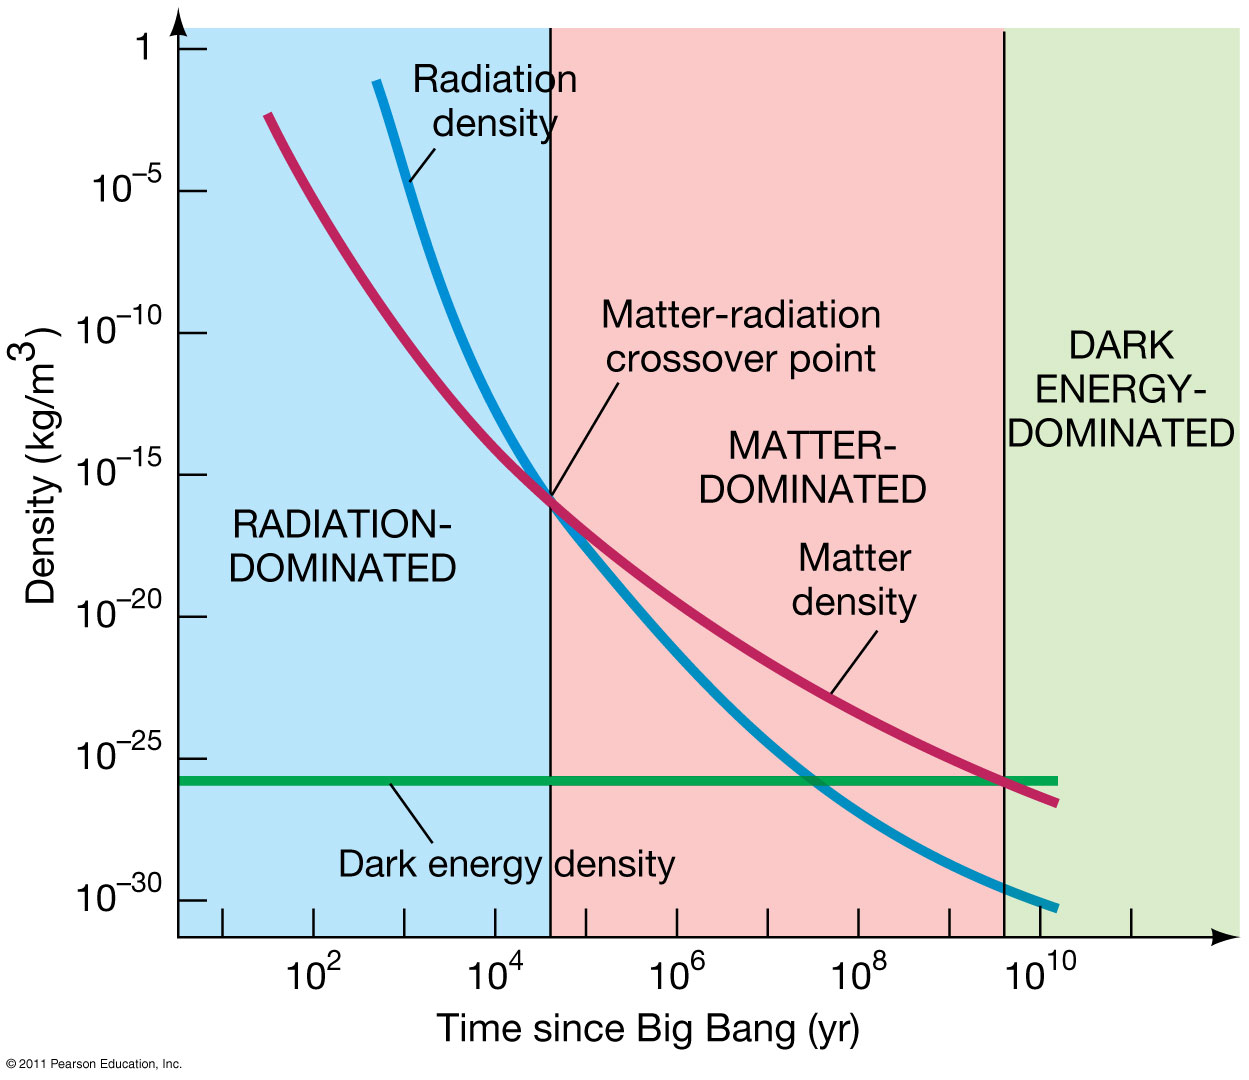
\includegraphics[width=0.7\textwidth]{Kosmo/2017/img/density.jpg}
	\caption{Densitet af hver komponent af universet som funktion af tid. Bemærk akserne er logaritmiske. Kilde: \cite{brauComponentsUniverse}.}
	\label{figDensity}
\end{figure}
%Billede fra http://pages.uoregon.edu/jimbrau/BrauImNew/Chap27/7th/AT\_7e\_Figure\_27\_01.jpg
%
Hvis vi kigger på ligning \eqref{friedmann_component}, så ser det ud til, at stråling og stof må have spillet en større rolle i universets barndom, end det gør i dag. Densiteten var højere (da a var lille) og det udgjorde en større andel af den samlede densitet, når vi husker på, at mængden af kosmologisk konstant per. rummængde er konstant. Selvom energien fra stråling er meget lav i dag, så falder den også hurtigst, og det betyder, at den engang har været dominerende (utroligt høj strålingsdensitet) i universet. Der skal vi selvfølgelig meget langt tilbage. Helt til universet kun var $47$ tusind år gammelt. Den kosmologiske konstant har domineret siden universet var $9.8$ mia. år gammelt, og i dag er det $13.8$ mia. år. Det er altså relativt kort tid (kun godt $4$ mia. år) siden  mørk energi begyndte at dominere. De forskellige perioder og densiteter er indtegnet på figur \ref{figDensity}.
Vi kan lave en approksimation og antage, at i hver fase vil skalafaktoren $a$ udvikle sig, som om universet kun består af den komponent, der dominerer.
%
\begin{figure}[t]
    \centering
    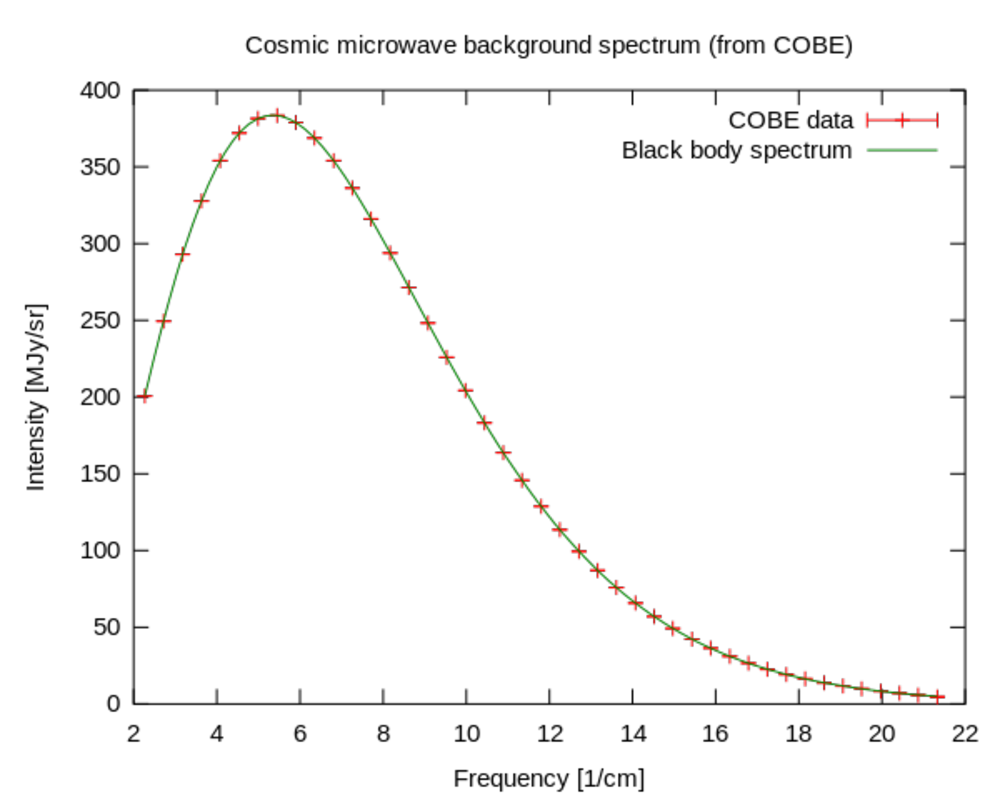
\includegraphics[width = .9\textwidth]{Kosmo/2017/img/cmbplanck.pdf}
    \caption{Et plot af målinger af baggrundsstrålingens frekvensspektrum med eksperimentet COBE, sammenlignet med et teoretisk sort-legeme spektrum for et objekt med samme temperatur. Variationen (samt usikkerhed) fra det forventede er lavere, end man kan plotte, selv med en forstørrelse af grafen. Kilde: \cite{CosmicMicrowaveBackground}.}
    \label{fig:cmbplanck}
\end{figure}

Udover disse faser, skete der en voldsom inflation lige i starten omkring $10^{-35}$ sekunder efter Big Bang. I løbet af dette tidsrum blev universet $10^{26}$ gange større. Det gik fra at være på størrelse med en proton til ca. en grapefrugt. Drivkraften menes at have været en anden form for kosmologisk konstant, der dominerede netop der, men senere blev overgået af stråling og stof. Massen fik så universets udvidelse til at deccelerere igen, indtil den kosmologiske konstant for nylig overtog. Baggrunden for denne teori er, at den forklarer hvorfor universet er så fladt (ujævnheder blev udjævnet) og hvorfor temperaturen er så ens overalt i det synlige univers. Man skulle tro at hver ende af det synlige univers aldrig ville have været i kontakt, så de ville ikke kunne udveksle energi. I det tilfælde vil der ikke være grund til at de skulle have samme temperatur. Alligevel er temperaturfordelingen i baggrundsstrålingen som samme sortlegeme (se figur~\ref{fig:cmbplanck}) overalt på Himlen. Det betyder at baggrundsstrålingen er varmestråling med samme temperatur overalt. Hvis alt lå virkelig tæt før inflationen, så kunne informationer og varme godt udveksles førhen. Det er altså en forklaring på, hvorfor det kosmologiske princip gælder i det synlige univers.
%\section{Universets skæbne}

\section{Mørkt Stof} \label{DM}
%Noget med rotationskurver af galakser, v af galakser i hobe, gravitational lensing

Ikke alene er det meste af det massen fra stof udetekterbart for vores øjne, men det er ikke nødvendigvis baryonisk heller. Størstedelen af stoffet i universet er ikke--baryonisk mørkt stof, hvilket betyder, at det ikke interagerer med den elektromagnetiske kraft, og derved hverken absorberer, emitterer eller spreder lys ved nogen bølgelængde. En måde hvorpå mørkt stof kan detekteres, er ved at se på dets gravitationelle indflydelse på synligt stof. En klassisk metode er at se på omløbshastigheden af stjerner i spiralgalakser. Mælkevejen er f.eks. en spiralgalakse. Tag nu Solen. Den er i en afstand $R=\SI{8.5}{\kilo\parsec}$ fra centrum af galaksen, og har en omløbshastighed på omkring $v=\SI{220}{km~s^{-1}}$. Solen vil opleve en centripetalacceleration
\begin{equation}
\Ddot{x} = \frac{v^2}{R} 
\end{equation}
mod centrum af galaksen. Hvis accelerationen $\Ddot{x}$ er givet ved gravitationel tiltrækning\footnote{Newtons universelle tyngdelov har samme afstandsafhængighed som Coulombs lov. Man kan således definere et tyngdefelt, der opfylder en version af Gauss' lov, se afsnit \ref{sec:gauss}, og dermed vise at ligning \eqref{eq:gravitationel_gauss} er sand.}, så er
\begin{equation} \label{eq:gravitationel_gauss}
\Ddot{x} = \frac{G M(R)}{R^2},
\end{equation}
hvor $M(R)$ er massen af galaksen indenfor en bestemt radius, $R$. De to ovenstående ligninger kan vi sætte lig hinanden for da at få et udtryk for hastigheden:
\begin{equation}
\frac{v^2}{R} = \frac{G M(R)}{R^2}
\end{equation}
eller
\begin{equation} \label{eq:fart_i_galakse}
v = \sqrt{\frac{G M(R)}{R}}.
\end{equation}
Vi kan måle hastigheden af stjerner i en galakse ved hjælp af deres rødforskydning fra Dopplereffekten. Nu ved vi, at hastigheden er større, desto større en masse stjernen kredser om. Altså kan vi beregne fordelingen af masse ved at kigge på stjerner forskellige steder i galaksen. Overfladelysstyrken, $I$, af disken i en spiralgalakse aftager med radius (det er den lysstyrke man ser, hvis man kigger på et område af galaksedisken ovenfra). Lysstyrken fortæller, os hvordan stjernerne dvs. synligt stof er fordelt.
\begin{equation}
I(R) = I(0) e^{-\frac{R}{R_\text{s}}},
\end{equation}
hvor $R_\text{s}$ er skalalængden (også kaldt den karakteristiske længde), som typisk ligger indenfor et par kiloparsec. $R_\text{s}$ er den afstand hvor $I$ er faldet med en faktor $e$. Vores galakse har $R_\text{s}\approx \SI{4}{kpc}$. Så snart du er et par skalalængder fra centrum af en spiralgalakse begynder massen af stjernerne indenfor $R$ af være konstant -- længere ude er der nemlig næsten intet lys. Hvis stjernerne bidrog til alt eller det meste af massen i en galakse, ville hastigheden falde af som $v \propto 1/\sqrt{R}$ ved store radier, fordi den indesluttede masse ville være nogenlunde konstant. Men det ser vi ikke. Hastighederne holder sig nogenlunde konstante, som på figur \ref{rotationskurve}, så der mangler noget masse. Faktisk mangler der mere masse, jo længere vi bevæger os ud (til en hvis grænse). Denne manglende masse kalder vi mørkt stof, da den ikke er synlig. At den ligger så langt ude er et tegn på, at massen ikke interagerer meget med hverken sig selv eller synligt stof, det er energitab fra interaktioner med andre partikler, der får stof til at `falde' ind mod centrum af galaksen. Derfor ligger det mørke stof stadig langt væk fra centrum, hvor det opretholder høje hastigheder. Det mørke stof interagerer dog gennem tyngdekraften, så det bliver stadig samlet i galaksers tyngdefelter. Denne komponent af galakser kalder vi deres \emph{dark matter halos}. De er sfæriske og ligger altså ikke kun i spiralgalaksens disk. \\

\begin{figure}[t]
	\centering
	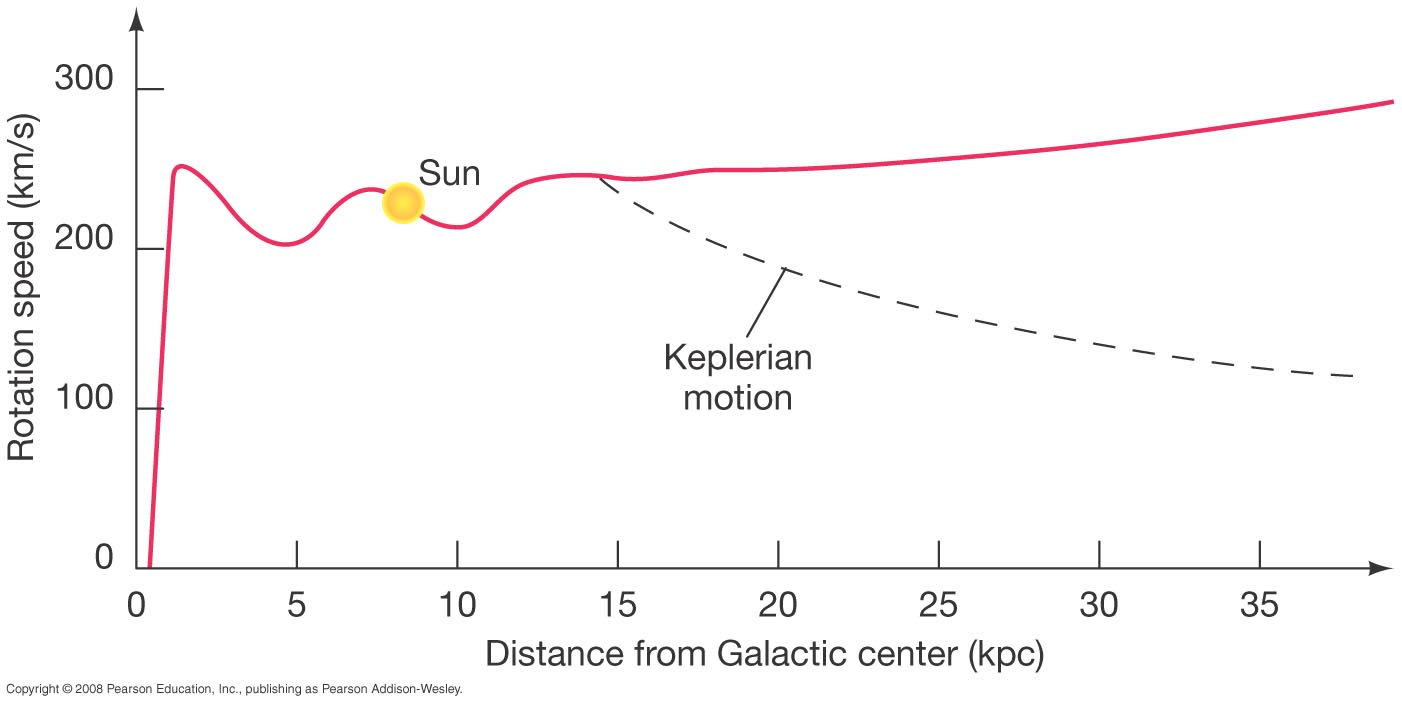
\includegraphics[width=0.7\textwidth]{Kosmo/2017/img/rotationskurve.jpg}
	\caption{Rotationskurve over Mælkevejen. Den solide kurve viser de observerede hastigheder, og den stiplede viser de forventede fra fordelingen af synligt stof. Afstanden mellem kurverne viser fordelingen af mørkt stof. Kilde: \cite{brauRotationMilkyWay}.
		}
	\label{rotationskurve}
\end{figure}
%Billede fra http://pages.uoregon.edu/jimbrau/BrauImNew/Chap23/6th/23\_21Figure-F.jpg

Man plejede at have to teorier for, hvad mørkt stof består af - WIMPs og MACHOs. WIMP står for Weakly Interacting Massive Particles og ville være en ny, tung type elementarpartikler. MACHO står for Massive Compact Halo Objects og er mere almindelige ting såsom sorte huller, svage dværgstjerner og `forældreløse' planeter, der er blevet slynget væk fra deres stjerner. Ting, der ikke lyser nok til, vi ville kunne se dem på lang afstand. Man har nu udelukket, at MACHOs kan udgøre en signifikant del af det mørke stof, da vi ville kunne se dets klumper af tyngdekraft deformere lyset af objekter bagved. Dette fænomen, kaldet \emph{gravitationslinseeffekten}, ses dog i mange andre sammenhænge f.eks. fra det mørke stof af en hel galakse. 

\iffalse
\subsection{Gravitationelle Linser}

En af konsekvenserne af generel relativitetsteori er, at et massivt objekt kan fungere som en linse, der bøjer lyset fra en fjernere kilde. F.eks. kan lyset fra et astronomisk objekt blive bøjet af tyngdefeltet fra en større mængde af masse (normalt samlet i galakser), der ligger mellem kilden og observatøren. Jo mere massiv en genstand er, desto større en linseeffekt ser vi. Derfor kan vi fra effekten regne os frem til massen af det mellemliggende objekt. Hvis det er en galakse, kan vi se, at den bøjer rummet meget mere end hvad den burde ud fra det synlige lys. Igen mangler der altså masse, og mørkt stof må eksistere.


Stærk lensing er når forvrængningen af f.eks. baggrundsgalakser, danner flere billeder af den samme galakse eller en hel ring rundt om det tunge objekt (også kaldet en Einstein ring). Dette har vi observeret omkring mange fjerne hobe, hvilket inkluderer den berømte Abell 1689, se Figur \ref{abell1689}. Ved måling af forvrængningsgeometrien (Eng: distortion geometry) kan massen af den mellemliggende hob findes. %I mange tilfælde, hvor man har gjort dette, opnåede man masse-til-lys forhold svarende til det dynamiske mørke stof målt i hoben.

Svag gravitationel lensing undersøger små forvrængninger ved hjælp af statistiske analyser fra store galakseundersøgelser. Ved at undersøge den tilsyneladende forskydningsdeformation af de tilstødende baggrundsgalakser, kan den gennemsnitlige fordeling af mørk stof karakteriseres.

Gravitationslinseeffekten kan også bruges til at opdage exoplaneter (planeter uden for Solsystemet). Det gælder, hvis lyset fra et objekt passerer en stjerne med en exoplanet, før det når frem til os. Så vil linsen forstærke lyset, og vi ser et ekstra lille bump fra planetens tyngdekraft.

\begin{figure}[h!]
	\centering
	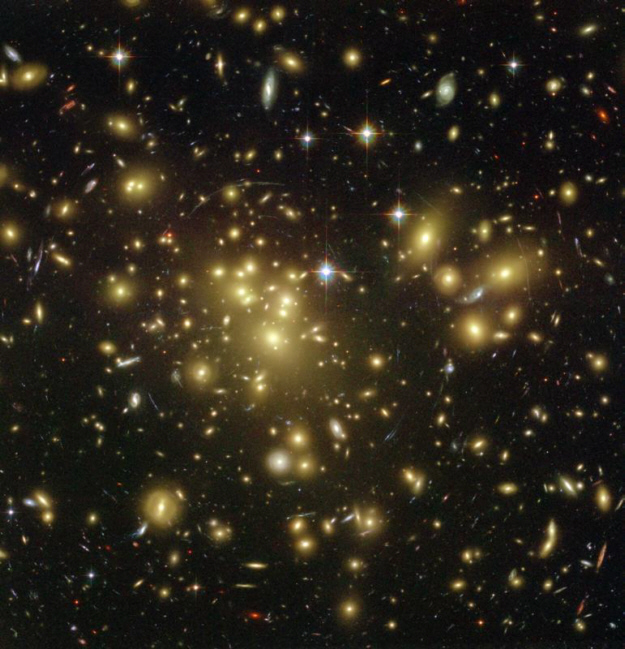
\includegraphics[width=0.6\textwidth]{Kosmo/2017/img/abell1689.jpg}
	\caption{Stærk gravitationel lensing observeret med Hubble Space Telescope, hvilket er en indikator for mørkt stof. Billede fra Hubble Space Telescope.}
	\label{abell1689}
\end{figure}
\fi

\section{Afstande og Luminositet}
Afstand er et vigtigt begreb i astrofysikken og kosmologien, men ofte også svært at måle. Derfor har vi mange forskellige typer afstandsmål, og hvordan de hænger sammen, er ikke altid fastlagt. En af de mest brugte metoder til bestemmelse af afstande er gennem et objekts \textit{luminositet}. Et objekts absolutte luminositet $L$ er defineret som den energi, der er udsendt per sekund. Det har vist sig, at en stjernes luminositet, hvis vi antager, at det er et sortlegeme, er relateret til dets radius $R$ og temperatur $T$:
\begin{equation}
L = 4\pi\sigma R^2T^4 \propto R^2 T^4
\end{equation}
hvor $\sigma$ er Stefan-Boltzmann's konstant. \\
Hvis denne energi er udsendt uniformt i alle retninger og modtages i en afstand $d_L$ væk, er den modtagede \textit{tilsyneladende luminositet} -- eller \emph{flux} -- givet ved:
\begin{equation} \label{eq:L}
F = \frac{L}{4\pi d_L^2},
\end{equation}
hvor $d_L$ er luminositetsafstanden. 

Et andet eksempel på et afstandsmål, er vinkelafstanden. Her kigger man simpelthen på hvor stor en vinkel, $\Delta \theta$, objektet udspænder på himlen. Metoden kræver adgang til en standardlineal dvs. et objekt hvis \textit{egenlængde}, $l$, er kendt. Egenlængden er den længde, man ville måle med en lineal fra den ene til den anden side. Standardlinealen skal være bundet godt sammen af enten tyngdekraften, gaffatape, eller måske en helt tredje kraft, som ikke tillader objektet at ekspandere med universet.  Vinkelafstanden, $d_\text{A}$, opskrives som
\begin{align}
	d_\text{A}=\frac{l}{\Delta \theta}.
\end{align}
For eksempel kan det antaget at galaksernes størrelse er fast i tid, og $l$ kan så være galaksernes faste størrelse, uafhængigt af afstanden til galaksen.
Udtrykkene for disse afstande er dog mest praktiske, når de er skrevet som funktion af $z$, da rødforskydningen altid er observerbar. De kan let blive skrevet som en funktion af skalafaktoren, $a$, samt andre parametre, ved at lave små og forholdsvis simple transformationer. For eksempel er de to udtryk for $d_L$ og $d_\text{A}$ næsten ens, men med en lille forskel:
\begin{align}
d_L(z) &= (1+z)d_\text{M}(z), \\
d_\text{A}(z) &=\frac{d_\text{M}(z)}{1+z},
\end{align}
hvor $d_\text{M}(z)$ afhænger af krumningen af universet. $d_\text{M}(z)$ kaldes på engelsk ''transverse comoving distance'', men lad os her blot betragte det som en faktor til at relatere rødforskydningen til andre afstandsmål. \\

Indenfor astronomiens verden beskrives et objekts lysstyrke ved \emph{magnitudesystemet}. Dette er et logaritmisk system, der rækker helt tilbage til Hipparchos i antikkens Grækenland. Af historiske årsager fungerer systemet således, at jo højere magnitude, desto svagere ser objektet ud på himlen og omvendt. Dengang fandtes der ikke teleskoper, som i dag, så alle målinger af stjerner blev taget per øjemål. Dengang gik skalaen fra 0 til og med 6, hvor 0 var det stærkeste på himlen og så fremdeles. Vi bruger i dag en skala, der er defineret således, at grækernes målinger stadig passer ind. Den tilsyneladende magnitude af et objekt vil variere med afstanden -- hvis man flytter sig tættere på en stjerne, vil den få en lavere magnitude (svarende til højere lysstyrke). Hvis man tager højde for afstanden, får man objektets absolutte magnitude, der er ens for alle observatører.

\subsection{Standard Candles}

Et standard candle\footnote{På dansk ser man nogle gange dette kaldt en standardlyskilde.} er et astronomisk objekt, der har en kendt absolut magnitude. Disse er super vigtige for astronomer, da man ved hjælp af den tilsyneladende magnitude af et objekt kan bestemme afstanden ved at bruge
\begin{equation}
m-M=5\cdot \log_{10}\left(\frac{d_L}{[\text{pc}]}\right) - 5 ,
\end{equation}
hvor $m$ er den tilsyneladende magnitude, $M$ er den absolutte magnitude, og $d_L$ er afstanden til objektet målt i parsec ([pc]). Forskellen kaldes objektets distancemodulus. Når der divideres med parsec, så er det blot for at fjerne længdeenheden, da man kun kan tage logaritmen til et tal uden enhed.

De mest anvendte standard candles indenfor astronomi er Cepheide variable stjerner og RR Lyræ stjerner. I begge tilfælde kan stjernernes absolutte magnituder bestemmes ud fra deres variabilitetsperioder. Med variable stjerner menes blot stjerner, hvis lysstyrke (eller tilsyneladende magnitude, set fra Jorden) ændrer sig over tid. Dette kan enten være grundet ændringer i stjernens luminositet/faktiske lysudsendelse (intrinsiske variable stjerner), eller ændringer i lyset efter udsendelse, for eksempel hvis det blokeres på vej mod os (ekstrinsiske variable stjerner). Cepheide variable stjerner og RR lyræ stjerner er typer af intrinsisk variable stjerner. 

Den nye dreng i klassen er Type Ia supernovaer. Disse kan også klassificeres som standard candles, men er i virkeligheden standardiserbare lyskilder, da de ikke har præcist den samme maksimale lysstyrke. Forskellene i deres maksimale lysstyrke er imidlertid korreleret med, hvor hurtigt lyskurven aftager efter maksimal lysstyrke. Her ser man på differencen mellem den maksimale lysstyrke og lysstyrken 15 dage efter. Dette kaldes også $\Delta m_{15}$. Hvis denne har en værdi mindre end $1$ er objektet lysstærkt, mens den ved en værdi over $1$ er lyssvagt.

\subsection{Olbers paradoks}
Lad os undersøge et simpelt spørgsmål –- hvorfor er nattehimlen mørk? Eller rettere -– hvorfor er den ikke uendeligt lys? Hvis vi lever i et uendeligt univers med en homogen og isotrop fordeling af stjerner, hvorfor ser vi så ikke uendeligt mange stjerner på himlen?

Vi kan opstille en formel for hvor meget lys vi modtager. Det må stige med antalsdensiteten af stjerner (stjerner per volumen) $n$, falde med afstanden fra os observatører, kaldet $r$, og stige med den flux af fotoner vi modtager fra hver stjerne, som vi kalder for $F$. Vi ønsker at finde intensiteten, $I$, som er den flux vi modtager per areal (hvor vi observerer) per rumvinkel på himlen. Dette er hvad vi rent fysisk forventer. \\

Den søgte formal kan vi finde, hvis vi grupperer alle stjerner efter hvor langt de er fra os. Dette gøres ved at betragte alle stjerne med en bestemt afstand, $r$, til os som værende på en kugleskal % Vi kan summe bidragene fra alle kugleskalle af stjerner, hvor hver skal har en 
med tykkelse $\dd r$. Det lille bidrag til den samlede intensitet, $\dd{I}$, er den mængde lys vi modtager fra hver stjerne, $F$, gange det antal stjerner, der er på kugleskallen, $N$. Antallet af stjerner på kugleskallen er antalstætheden, $n$ gange volumen af kugleskallen, $V_\mathrm{skal} = 4\pi r^2 \dd r$. Dermed bidrager kugleskallen med intensiteten
\begin{align}
	\dd I = FN = Fn4\pi r^2\dd r %Hvorfor ikke 4pir^2?
\end{align}
Her kan vi indsætte udtrykket for $F$ fra afstandskvadratloven \ref{eq:L}, hvor afstanden $d_L = r$ %Tjek at vi har nævnt den først
\begin{align}
	\dd I = \frac{L}{4\pi r^2} 4\pi nr^2\dd r = L n \dd r. 
\end{align}
For at finde den totale intensitet vi hver skal som værende infinitesimalt tynd og integrerer over hele det uendelige univers:
\begin{align}
	I =\int^\infty_0 Ln \dd{r}
\end{align}
Her er en masse konstanter, der ikke vil ændre sig som funktion af radius, så dem kan vi trække ud af integralet
\begin{align}
	I = Ln \int^\infty_0 \dd r = L n \big[r\big]_0^\infty = L n \big(\infty - 0\big) = \infty.
\end{align}
Ergo må universet være uendeligt lyst.  Dette holder som bekendt ikke i virkeligheden, da der faktisk ligger en del antagelser bag udledningen. Tag gerne et øjeblik til at overveje, hvad du tror årsagen er.

Det kunne f. eks. være universet ikke er homogent, så der kun findes stjerner tæt på os, eller dem langt væk lyser mindre. Det har vi dog ingen anden grund til at tro er tilfældet. Men hvis $nL \propto \frac{1}{r^x}$, for $x>1$, så kan himlen være mørk.

Det kunne også være universets krumning betyder, at vi ikke kan bruge afstandskvadratloven, så flux falder hurtigere med afstand. Det ser vi dog ingen tegn på indtil videre.

En tredje antagelse, er at vi kan se alle stjerner, uden andre objekter kommer i vejen for vores synslinjer. Hvis stjernerne skygger for hinanden, så bliver himmelen ikke uendeligt lys, men får en jævn lysstyrke som overfladen på en stjerne, hvilket stadig ikke giver en mørk himmel. Andet materiale kunne også skygge for stjernerne, men det ville i så fald absorbere lys, indtil det udsender lige så meget energi, som det absorberer. Det vil sige, at det også ville lyse lige så kraftigt som stjernerne, hvorfor det løser heller ikke problemet.

For det fjerde, kunne det være universet ikke er uendelig stort, så der ikke er nogen stjerner efter en hvis radius.

Hvis universet udvider sig så hurtigt, at stjerners lys rødforskydes nok til vi ikke kan opfange det, så vil det også gøre himlen mørk. 

Den primære løsning til Olbers paradoks er dog, at universet ikke er uendeligt gammelt. Det betyder, at lyset fra fjerne stjerner simpelthen ikke er nået frem til os endnu.


% Vi kan opstille en formel for hvor meget lys vi modtager. Det må stige med antalsdensiteten af stjerner (stjerner per volumen) $n$, falde med afstanden fra os observatører, kaldet $r$, og stige med den flux af fotoner vi modtager fra hver stjerne, som vi kalder for $F$. Vi ønsker at finde intensiteten, $I$, som er den flux vi modtager per areal (hvor vi observerer) per rumvinkel på himlen.

% Det kan vi finde, hvis vi grupperer alle stjerner efter hvor langt de er fra os. Vi kan summe bidragene fra alle kugleskalle af stjerner, hvor hver skal har en tykkelse $\dd r$. Det lille bidrag til den samlede intensitet er da
% \begin{align}
% 	\dd I = Fnr^2\dd r %Hvorfor ikke 4pir^2?
% \end{align}
% Her kan vi indsætte udtrykket for $F$ fra afstandskvadratloven \ref{eq:L} %Tjek at vi har nævnt den først
% \begin{align}
% 	\dd I = \frac{L}{4\pi r^2} nr^2\dd r = \frac{L}{4\pi} n \dd r. 
% \end{align}
% For at finde summen af alle bidragene fra kugleskallerne, gør vi hver skal infinitesimalt tynd og integrerer over hele det uendelige univers:
% \begin{align}
% 	I =\int^\infty_0 \frac{L}{4\pi r^2} nr^2 \dd{r}
% \end{align}
% Her er en masse konstanter, der ikke vil ændre sig som funktion af radius, så dem kan vi trække ud af integralet
% \begin{align}
% 	I =\frac{L}{4\pi r^2} n \int^\infty_0 r^2 \dd{r} =\frac{L}{4\pi r^2} n \cdot \infty = \infty
% \end{align}
% Ergo må universet være uendeligt lyst.  Dette holder som bekendt ikke i virkeligheden, da der faktisk ligger en del antagelser bag udledningen.

% \newpage
% \section{Opgaver}

\begin{opgave}{Hubbleloven}
    \opg Forklar hvorfor Hubbleloven kun gælder hvis $v>0$.
    \opg Kan Hubbleloven bruges til at bestemme afstande til himmellegemer, hvis lys er er blåforskudt?
\end{opgave}

\begin{opgave}{Den kritiske tæthed}
Den kritiske tæthed, $\rho_c$, kan defineres ud fra Friedmannligningen som den værdi af $\rho$, der opfylder ligning \eqref{friedmann} for et fladt univers.
\opg Hvilken værdi har $\kappa$ i et fladt univers?
\opg Vis at den kritiske tæthed er
%
\begin{align}
    \rho_c = \frac{1}{8\pi G}\left(3H^2 - \Lambda\right).
\end{align}
%
\opg Argumenter for at hvis $\Lambda \ll 3H^2$ så er
%
\begin{align} \label{eq:rho_c}
    \rho_c \simeq \frac{3H^2}{8\pi G}.
\end{align}
%
\opg Brug ligning \eqref{eq:rho_c} til at vise at den kritiske tæthed i Universet med den nuværende værdi af Hubbleparameteren, $H_0$, er
%
\begin{align*}
    \rho_\text{c} = \SI{8.6e-27}{\kilo\gram\per\cubic\metre}.
\end{align*}
\end{opgave}

\begin{opgave}{Et Univers af bolde}
Massetætheden i et univers kun bestående af bolde med massen $m_\mathrm{b} = \SI{1}{M_\odot}$ er
%
\begin{align} \label{eq:antalsdensitet}
    \rho = n_\mathrm{b}m_\mathrm{b},
\end{align}
%
hvor $n_\mathrm{b}$ er antalstætheden af bolde -- det vil sige antallet af bolde per volumen.
\opg Hvad skal antalstætheden af bolde være for at universet har den nuværende kritiske tæthed $\rho_\text{c} = \SI{8.6e-27}{\kilo\gram\per\cubic\metre}$?
\opg Den gennemsnitlige afstand mellem bolde i et sådant univers skalerer som $d_\mathrm{b} = n_\mathrm{b}^{-1/3}$. Bestem denne afstand.
\opg De fjerneste galakser vi kan se er i en afstand fra Jorden på $d_\mathrm{max} \approx \si{\clight}/H_0$. Bestem $d_\mathrm{max}/d_\mathrm{b}$.
\opg Er det sandsynligt at kunne se på den afstand vi kan, hvis vi levede i et univers af sådanne bolde? Advarsel: Denne opgave har intet facit, da radius af boldene ikke er oplyst. Men prøv gerne at opstille et generelt udtryk for sandsynligheden for at kunne se til afstand $s$, når man kigger i en tilfældig retning og boldene har radius $r$.

\opg Havde man brugt Mælkevejens masse, $m_\mathrm{b} = \SI{1e12}{M_\odot}$, ville man få $d_\mathrm{max}/d_\mathrm{b} = \SI{2.2e3}{}$, mens massen for en typisk galaksehob, $m_\mathrm{b} = \SI{1e15}{M_\odot}$, giver $d_\mathrm{max}/d_\mathrm{b} = \SI{2.2e2}{}$. Hvad fortæller disse udregninger os om Universet? Advarsel: Denne opgave har intet facit, da radius af boldene ikke er oplyst.
\end{opgave}

\begin{opgave}{Dopplerforskydning}%{2}
	Formlen for frekvensen ved Dopplerforskydning er
	\begin{align}
		f_{obs} = \frac{c+v_{obs}}{c+v_{kilde}} f_{kilde},
	\end{align}
	hvor $c$ er lydens hastighed i mediet, $f_{obs}$ er den observerede frekvens (udefra), $f_{kilde}$ er den udsendte frekvens, $v_{obs}$ er observatørens hastighed og $v_{kilde}$ er kildens hastighed.
	\opg En politibil kører mod dig 30 meter væk, men er 20 meter fra centrum af vejen når du kigger ligeud (se skitsen på Figur \ref{politi}). Tegn hastighedsvektoren og hastighedskomponenterne der peger henholdsvis parallelt med din synsvinkel og vinkelret på den. 
	\opg Bilens speedometer viser, at den kører 50 km/t. Brug trigonometri til at beregne hvor stor en hastighedskomponent, der peger mod dig (radiel hastighed). Skitsér groft en graf over radiel hastighed som funktion af tid og antag, at bilens hastighed er konstant.
	\opg Politibilens sirene udsender lyd med en frekvens på 800 Hz. Du står stille, og det er en let kølig dag med 15 grader, hvor lydens fart i luft er 340 m/s. Ved hvilken frekvens hører du tonen?
	\begin{figure}[h!]
		\centering
		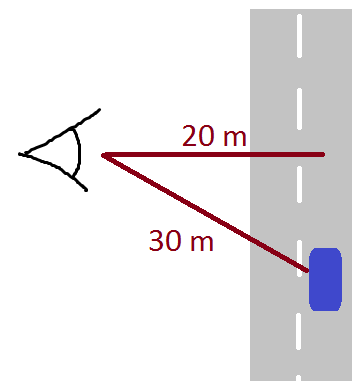
\includegraphics[width=0.5\textwidth]{opg/figurer/Politi.png}
		\caption{}
		\label{politi}
	\end{figure}
\end{opgave}

\begin{opgave}{Skalafaktor}%{1}
	Temperaturen af den kosmiske mikrobølgebaggrund er i dag 2.73 K. Strålingen blev udsendt ved "rekombinationen", hvor universet var koldt nok til at elektroner kunne binde sig til atomkernerne. Det var en mindre exciteret tilstand, så atomerne udsendte energi som fotoner. Man kan måle, at det har krævet en temperatur på kun 3000 K. Brug at temperaturen udviklede sig som
	\begin{align}
		T(t)=\frac{T_0}{a(t)}
	\end{align}
	til at finde ud af, ved hvilken rødforskydning rekombinationen fandt sted.
\end{opgave}

\begin{opgave}{Rødforskydning af kvasar}%{1}
	Kvasarer (eng:”quasars” fra ”quasi-stellar radio sources”) er de mest energirige og
	fjerne medlemmer af objekterne kendt som aktive galaksekerner (eng:”AGN: Active
	Galactic Nuclei”). Kvasarer har siden deres opdagelse været omgivet af mystik, men
	der er nu opnået generel enighed om, at de er kompakte regioner i massive galakser,
	der indeholder det centrale supermassive sorte hul. De kæmpe mængder energi der
	bliver udstrålet af kvasarerne stammer fra al stoffet, som falder ind mod det sorte
	hul og bliver slynget ud.
	Et kvasar-spektrum er vist i Figur \ref{kvasar}.
	\\
	I Balmer-serien hopper en elektron til 2. orbital fra en mere exciteret tilstand. Den første af disse kaldes H-$\alpha$ og er faldet fra orbital 3 til 2. Den næste er H-$beta$ fra orbital 4 til 2 osv. Fotoner, der udsendes ved H-$\alpha$-overgangen, har en bølgelængde på 656 nm. Ofte måler man i ångstrøm (Å) som er $10^{-10}$ m.\\
	%Aflæs bølgelængden for H-$\beta$ på Figur \ref{spektrum} og beregn rødforskydningen.
		\begin{figure}[h!]
			\centering
			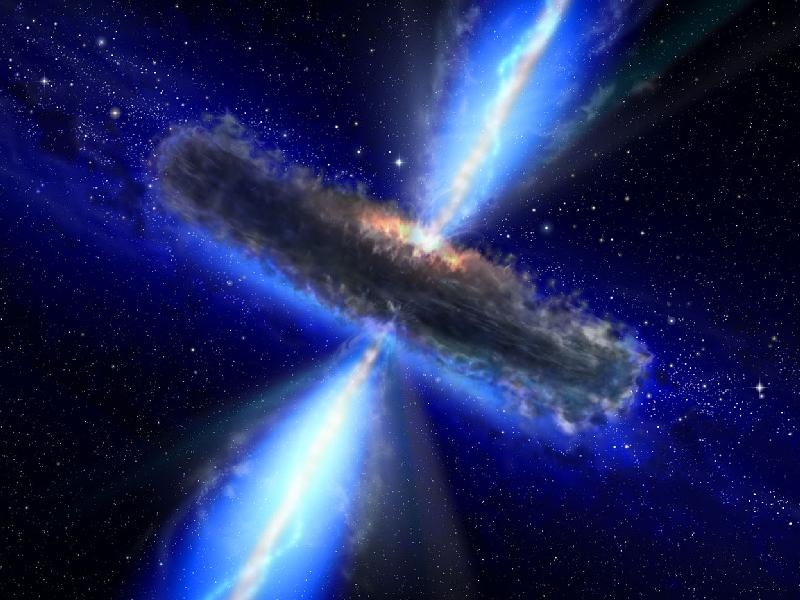
\includegraphics[width=0.5\textwidth]{opg/figurer/kvasarkunst.jpg}
			\caption{En kunstnerisk forestilling af en kvasar. Kilde: \cite{NASA_ESA_quasar}} %https://pbs.twimg.com/profile_images/683524276058763264/xyAc-NvD.jpg
			\label{kvasarkunst}
		\end{figure}
	\begin{figure}[h!]
		\centering
		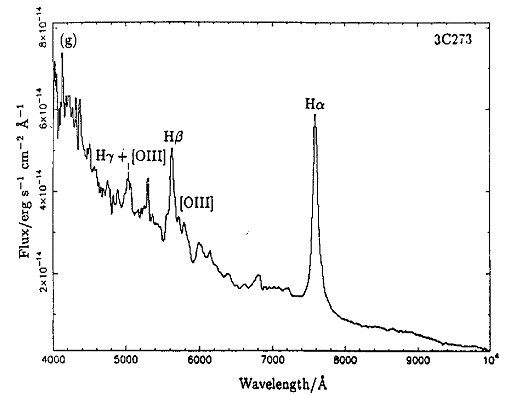
\includegraphics[width=0.5\textwidth]{opg/figurer/kvasar.png}
		\caption{Spektrum af kvasaren 3C273. Kilde: \cite{YatesGardenQuasarSpectrum}} %http://www.astrosurf.com/buil/us/spe6/qso1.gif
		\label{kvasar}
	\end{figure}
	\opg Ud fra din viden om H-$\alpha$-overgangen, bevæger kvasaren sig så mod eller væk fra os?
	\opg Hvad er kvasarens radielle hastighed?
	\opg Man ser tit, at spektrallinjerne fra kvasarer er meget brede, fordi gassen bevæger sig hurtigt omkring det sorte hul, hvilket giver en Doppler-forbredning
	(lyset bliver både rød- og blåforskudt). Estimér bredden af H-$\alpha$-linjen, $\Delta\lambda_{obs}$, og udregn gassens fart ved 
	\begin{align}
		v_{gas}=\frac{\Delta \lambda_{obs}}{2\lambda_{0}}c
	\end{align}
\end{opgave}

\begin{opgave}{Afstande} %{3}
	\\  		
	\begin{figure}[h!]
			\centering
			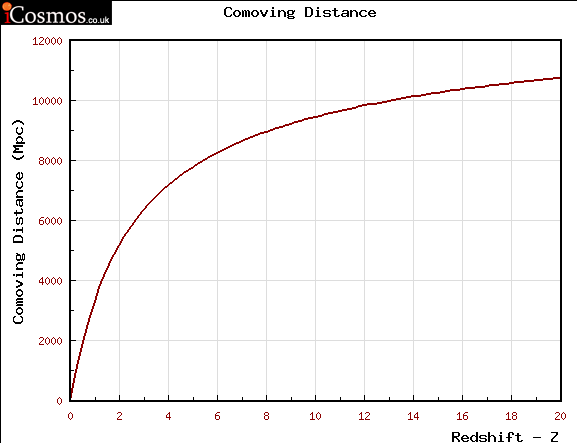
\includegraphics[width=0.5\textwidth]{opg/figurer/ComovingDistance.png}
			\caption{Kilde: \cite{vardanyanICosmosCosmologyCalculator}.} %http://www.icosmos.co.uk/index.html
			\label{comoving} 
		\end{figure}
	\opg Opskriv luminositetsafstanden $D_L$ som funktion af vinkelafstanden $D_A$.
	\opg I et fladt univers er $D_M=D_C$. $D_C$ kaldes comoving distance, og med $\Omega_m=0.3$ og $\Omega_{\Lambda}=0.7$ opfører det sig som plottet på Figur \ref{comoving}. 
	Hvor stor er $D_L$ og $D_A$ ved $z=1$? \\
	Hvad med ved $z=9$? Giver ændringerne mening?
	\opg Hvor stor er den radielle hastighed for et objekt med $z=10$? Oplys svaret som procent af lysets fart i vakuum. Dengang var universet for resten kun  478 mio. år gammelt.
\end{opgave}

\begin{opgave}{Andromeda-galaksen}
		\begin{figure}[h!]
			\centering
			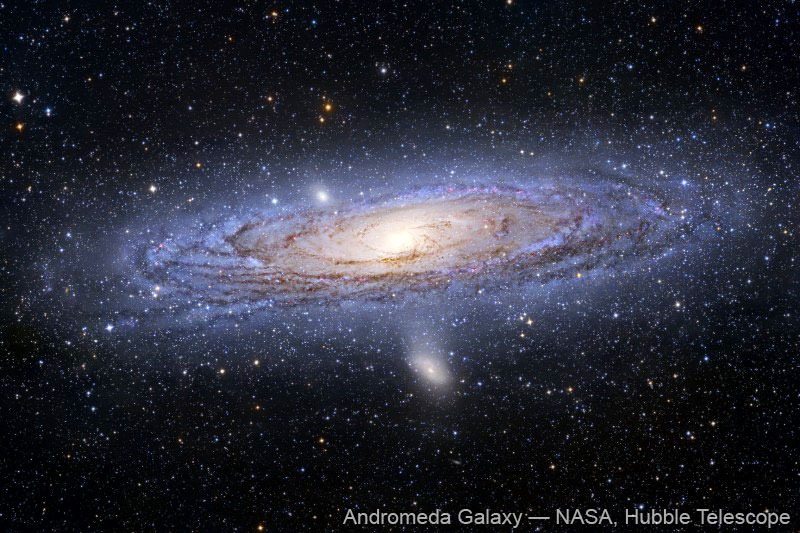
\includegraphics[width=0.5\textwidth]{opg/figurer/andromeda.jpg}
			\caption{Kilde: \cite{AndromedaGalaxy2019}.} %https://upload.wikimedia.org/wikipedia/commons/9/98/Andromeda_Galaxy_%28with_h-alpha%29.jpg
			\label{andromeda} 
		\end{figure}\\
	Andromeda-galaksen eller Messier-31 (M31) er den nærmeste spiralgalakse, og den største galakse i den Lokale Gruppe, som er en samling af ca. 50 galakser, heriblandt vores egen, Mælkevejen.  
	\opg Det observerede lys fra Andromeda har en rødforskyning på $z = -0.001$.
	%\opg Det observerede lys fra Andromeda har en rødforskydning på $z = −0.001$.
	Hvad er Hubbleafstanden til galaksen, fundet ved hjælp af Hubbles lov? Antag Hubblekonstanten er $H_0=70 km s^{-1} Mpc^{-1}$.
	\opg Gennem andre metoder har man fundet afstanden til 2,5 mio. lysår. Hvornår støder Andromeda og Mælkevejen sammen? Hvad tror du, det kommer til at betyde? Antag hastigheden er konstant, og Andromeda har direkte kurs mod os.
\end{opgave}




%\chapter{Astrofysik Facitliste}
%\section*{Astrofysik}

% \newpage
% \section{Facit}

\begin{opgave}{Hubbleloven}
    \opg Hubbleloven beskriver universets udvidelse, der får alting til at bevæge sig væk fra hinanden. Negative hastigheder betyder at himmellegemer bevæger sig imod os, hvilket ikke kan skyldes universets udvidelse. Ergo gælder Hubbleloven kun for objekter med $v > 0$. Hvis man prøvede alligevel ville man få en negativ længde, og det giver ikke mening.
    \opg Lys bliver blåforskudt, når lyskilden bevæger sig imod modtageren. Af spørgsmål \textbf{1}) gælder Hubbleloven derfor ikke.
\end{opgave}

\begin{opgave}{Den kritiske tæthed}
\opg Hvis universet er fladt har det ingen krumning, hvorfor $\kappa = 0$
\opg Indsættes $\kappa = 0$ i Friedmannligningen fås
%
\begin{align*}
    H^2 &= \frac{8\pi G \rho}{3} + \frac{\Lambda}{3}, \\
    \implies H^2 - \frac{\Lambda}{3} &= \frac{8\pi G}{3}\rho.
\end{align*}
%
Ganges brøken over fås
%
\begin{align*}
    \rho_c = \frac{1}{8\pi G}\left(3H^2 - \Lambda\right).
\end{align*}
%
\opg $\Lambda \ll 3H^2 \implies 3H^2 - \Lambda \simeq 3H^2$ hvorfor
%
\begin{align*}
    \rho_c \simeq \frac{3H_0^2}{8\pi G}.
\end{align*}
%
\opg Bruges værdierne $H_0 = \SI{67.7}{\kilo\meter\per\second\per\mega\parsec}$ og $G = \SI{6,6742e-11}{\newton\square\metre\per\square\kilo\gram}$ fås
%
\begin{align*}
    \rho_\text{c} \simeq \frac{3H_0^2}{8\pi G} = \frac{3(\SI{67.7}{\kilo\meter\per\second\per\mega\parsec})^2}{8\pi\cdot\SI{6,6742e-11}{\newton\square\metre\per\square\kilo\gram}} =  \SI{8.6e-27}{\kilo\gram\per\cubic\metre}.
\end{align*}
\end{opgave}

\begin{opgave}{Et univers af bolde}
\opg Isoleres $n_\mathrm{b}$ i ligning \eqref{eq:antalsdensitet} og indsættes værdierne $m_\mathrm{b} = \SI{1}{M_\odot}$ og $\rho_\text{c} = \SI{8.6e-27}{\kilo\gram\per\cubic\metre}$ fås
%
\begin{align*}
    n_\mathrm{b} = \frac{\rho_\mathrm{c}}{m_\mathrm{b}} = \frac{\SI{8.6e-27}{\kilo\gram\per\cubic\metre}}{\SI{1}{M_\odot}} = \SI{4,3e-57}{\per\cubic\metre}.
\end{align*}
\opg Indsættes ovenstående resultat fås
%
\begin{align*}
    d_\mathrm{b} = n_\mathrm{b}^{-1/3} = (\SI{4,3e-57}{\per\cubic\metre})^{-1/3} = \SI{198.9}{\parsec}.
\end{align*}
\opg Indsættes værdierne $d_\mathrm{b} = \SI{198.9}{\parsec}$, $H_0 = \SI{67.7}{\kilo\meter\per\second\per\mega\parsec}$ og $\si{\clight} = \SI{2.99792e8}{\metre\per\second}$ fås
%
\begin{align*}
    \frac{d_\mathrm{max}}{d_\mathrm{b}} = \frac{\si{\clight}/H_0}{d_\mathrm{b}} = \frac{\SI{2.99792e8}{\metre\per\second}/\SI{67.7}{\kilo\meter\per\second\per\mega\parsec}}{\SI{198.9}{\parsec}} = \SI{2.2e7}{}.
\end{align*}
\opg Denne delopgave kan ikke løses, da størrelsen af boldene ikke er oplyst. Hvis den var, kunne man beregne sandsynligheden for at en foton i en given retning fra os vil ramme en bold inden for en bestemt radius. Det gøres ved at for hver kugleskal af himlen i en bestemt radius fra os, og med en lille tykkelse dx, kan man finde et gennemsnitligt antal bolde, da vi kender deres tæthed. Sandsynligheden for at en foton bliver stoppet i denne kugleskal, er så arealet dækket af bolde divideret med det totale areal. Man kan integrere over disse kugleskaller, for at finde den totale sandsynlighed for at blive stoppet inden for en radius $s$, som man integrerer ud til (ligesom i eksemplet med Olbers paradoks). Så spørgsmålet kan omformuleres til: Hvad er sandsynligheden for at en fotons bane fra os brydes inden radius $d_{max}$, antaget en bestemt boldradius $r$? %Det kosmologiske princip siger, at universet er homogent og isotropt -- altså at massen er jævnt fordelt over hele universet, og at det ser ens ud i alle retninger. Hvis vi skal kunne se noget i afstanden $d_\mathrm{max}$ i et univers kun bestående af bolde, så skal der være et retning, hvor den nærmeste bold er i den afstand. Skal man kunne se cirka 22 millioner gange længere end den gennemsnitlige afstand mellem bolde, så svarer det løst sagt til at der mangler 22 millioner bolde i en bestemt retning, og de må jo så være et andet sted i universet. Det ville dog betyde at der er forskel på hvilken retning vi kigger i, og at massetætheden ikke er den samme alle steder. Det er derfor usandsynligt, at have et univers bestående af sådanne ens bolde, hvor universet har den nuværende massetæthed, hvor vi kan se noget i afstanden $d_\mathrm{max}$, mens det kosmologiske princip er gældende. Det er ikke direkte i modstrid med det kosmologiske princip, da \SI{2,2e7}{M_\odot} ikke er voldsomt stort på kosmologisk skala -- til sammenligning er massen af mælkevejen $\sim \SI{1e12}{M_\odot}$ -- men det er stort nok til at være betydningsfuldt.
\opg Denne delopgave kan ikke løses, da størrelsen af boldene ikke er oplyst. %Hele udregningen byggede på en antagelse om at universet kun består af består af bolde med massen $m_\mathrm{b} = \SI{1}{M_\odot}$. Denne antagelse har svært ved at forklare den afstand vi kan se i universet, hvorfor der må være noget galt med antagelsen. Det mest oplagte er tyngdekraften får masse til at klumpe sig sammen til objekter, der er tungere end 1 solmasse. Dette ses også ved den markante forbedring af $d_\mathrm{max}/d_\mathrm{b}$ ved at bruge Mælkevejens masse. På stor skala er Universet altså bedre beskrevet som en samling af ens galakser end en samling af ens stjerner. Dette viser også at det kosmologiske princip fungerer på store længde skalaer, men ikke på mindre. Det er eksempelvis ikke sandt, at alle dele af Mælkevejen ser ens ud fra Jorden -- der er langt mere masse, hvis vi kigger mod galaksens centrum, end hvis vi kigger i den modsatte retning. Galakser samler sig også i galaksehobe, og bruges massen for sådan en fås, at vi kan se cirka 200 gange længere end den gennemsnitlige afstand mellem bolde i et univers hvor boldene vejer det samme som en galaksehob. Dette tyder på, at universet skal det beskrives på en skala af galakser og galaksehobe. Modellen tager ikke højde for at boldene kan have forskellig masse og derudover er synslængde ikke nok i sig selv til at kunne afgøre om modellen er brugbar. Det virker dog sandsynligt, at Universet på tilpas stor skala opfører sig som en samling af galakser og galaksehobe, da det kosmologiske princip lægger op til, at en model med ens bolde ikke er helt ved siden af.
\end{opgave}

\begin{opgave}{Dopplerforskydning}
	\opg 
	\begin{figure}[h!]
		\centering
		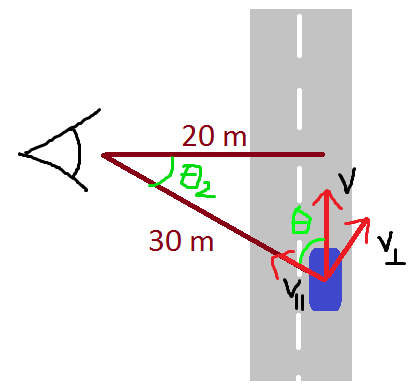
\includegraphics[width=0.5\textwidth]{opg/figurer/PolitiLoesning.png}
		%\caption{Et typisk } %https://upload.wikimedia.org/wikipedia/commons/9/98/Andromeda_Galaxy_%28with_h-alpha%29.jpg
	\end{figure}
	\opg Den radielle hastighed er den parallele komponent med synsvinklen. Vi ser en retvinklet trekant og bruger
	\begin{align}
		\cos(\theta)=\frac{\text{hosliggende katete}}{\text{hypotenusen}}=\frac{v_{radiel}}{v} \\
		v_{radiel}=v \cos(\theta)
	\end{align}
	Der dannes også en retvinklet trekant af vejen, afstanden til vejen og afstanden til bilen. I grader giver det en vinkel på
	\begin{align}
		\cos(\theta_2)&=\frac{20}{30}\\
		\theta_2 &= \cos^{-1} \left( \frac{20}{30} \right) = 48
	\end{align}
	De to vinkler indgår begge i en retvinklet trekant, så
	\begin{align}
		180 &= \theta + \theta_2 + 90\\
		\theta &= 90 - \theta_2  = 42
	\end{align}
	Vi indsætter og får
	\begin{align}
	v_{radiel}=50 km/t \cdot \cos(42) = 50 km/t \cdot 0.74 = 37 km/t
	\end{align}
	Hvis du ikke får det samme, så prøv at regne alt i radianer, da det er simplere.
	\opg 
	Du står stille, så $v_{kilde}=0$. $v_{obs}$ er den radielle hastighed, som lige skal omregnes til km/t:
	\begin{align}
	37 km/t = 37 \frac{10^{3}m}{60\cdot60 s} = \frac{37}{3.6} m/s = 10.3 m/s
	\end{align}
	Så indsætter vi i
	\begin{align}
	f_{obs} = \frac{340 m/s + 10,3}{340 m/s + 0} 800 Hz = 824 Hz
	\end{align}
    (Hz er enheden hertz, som er 1/s)
\end{opgave}

\begin{opgave}{Skalafaktor}
	Vi ved temperaturen dengang var $T(t) = 3000 K$ og nu er den $T_0 = 2.73 K$. Så vi kan bruge at skalafaktoren ændrer sig med rødforskydningen, og sammensætte det med hvordan den ændrer sig med temperatur:
	\begin{align}
	    a(t) = \frac{1}{1+z} = \frac{T_0}{T(t)}\\
	    z = \frac{T(t)}{T_0} - 1
	\end{align}{}
	Så vi kan nu regne fra temperatur til rødforskydning:
	\begin{align}
	    z = \frac{T(t)}{T_0} - 1 = \frac{3000 K}{2.73 K} - 1= 1,10\cdot10^3 -1 \approx 1,10\cdot10^3
	\end{align}
	Så der blev dannet atomer ved $z\approx1100$, da det blev koldt nok til elektroner kunne binde sig til atomkernenerne.
\end{opgave}

\begin{opgave}{Rødforskydning af kvasar}
	\opg nm er $10^{-9} m= 10 \cdot 10^{-10} m$, så H-$\alpha$-linjen er ved ca. $6560$ Å. På figur \ref{kvasar} er det ved omkring $7600$ Å, dvs. bølgelængden er blevet større, så lyset er rødforskudt. Altså må kvasaren bevæge sig væk fra os.\\
	\opg Den radielle hastighed er beskrevet af rødforskydningen. Rødforskydningen er
	\begin{align}
		\frac{\lambda_{obs}-\lambda_{lab}}{\lambda_{lab}} = \frac{7600-6560}{6560} = 0,159.
	\end{align}
	Det er lavt, så vi approksimerer hastigheden til
	\begin{align}
		v= z\cdot c = 0,159 \cdot 3\cdot 10^8 \frac{m}{s}= 4,7\cdot 10^7 \frac{m}{s}
	\end{align}
	Regner du det præcist, giver det nogenlunde det samme.
	\opg $\Delta\lambda \approx 200 Å$, så det giver $v=0.015 c = 4,5\cdot 10^6 m/s$.
\end{opgave}
\begin{opgave}{Afstande}
	\opg Isolér $D_M$ i hvert udtryk.
	\begin{align}
		D_M &= \frac{D_L}{1+z}\\
		D_M &= D_A(1+z)
	\end{align}
	Resultaterne sættes lig hinanden
		\begin{align}
		\frac{D_L}{1+z} &= D_A(1+z)\\
		D_L &= D_A (1+z)^2
		\end{align}
	\opg Ved $z=1$ er $D_C\approx3200 Mpc$ og derfor
	\begin{align}
		D_L &= D_M(1+z)= 3200 Mpc \cdot 2 = 6400 Mpc\\
		D_A &= \frac{D_M}{1+z}= 3200 Mpc/ 2 = 1600 Mpc.
	\end{align}
	Ved $z=9$ er $D_C\approx9200 Mpc$, så
	\begin{align}
		D_L &= D_M(1+z)= 9200 Mpc \cdot 10 = 92000 Mpc\\
		D_A &= \frac{D_M}{1+z}= 9200 Mpc/ 10 = 920 Mpc.
	\end{align}
	Gamle objekter, der har bevæget sig fra os længere tid, har altså en større luminositetsafstand, men en lavere vinkelafstand ved høje rødforskydninger. Man skulle ellers tro objekter så mindre ud på himlen, jo længere væk de var, hvilket er rigtigt indtil omkring $z=1,6$. I det tidlige univers var galakserne tættere på hinanden, så de fyldte meget på himlen for hinanden, og derfor er deres lys spredt ud over et stort område.
	\opg
	%Dengang var universet for resten kun 250 mio. år gammelt.\\
	Hvis vi approksimerer $z\approx\frac{v}{c}$, får vi overlyshastigheder, så det går ikke.
	\begin{align}
    	z+1&=\sqrt{\frac{1+\frac{v}{c}}{1-\frac{v}{c}}}\\
    	(z+1)^2&=\frac{1+\frac{v}{c}}{1-\frac{v}{c}}
	\end{align}
	så vi skal løse et system på formen $y=\frac{1+x}{1-x}$, hvor $y=(z+1)^2$ og $x=\frac{v}{c}$. Man kan omformulere det til $x=\frac{y-1}{y+1}$, ved
	\begin{align}
	    1+x &= y(1-x)\\
	    1+x &= y-yx \\
	    x+yx &= y-1 \\
	    x(1+y) &= y-1 \\
	    x &= \frac{y-1}{y+1}.
	\end{align}
    Derfor må
	\begin{align}
    	\frac{v}{c}&=\frac{(z+1)^2-1}{(z+1)^2+1}\\
    	v&=\frac{(z+1)^2-1}{(z+1)^2+1} c = \frac{(10+1)^2-1}{(10+1)^2+1} = 0.98 c. %3\cdot 10^{8} m/s =
	\end{align}
	Så svaret er 98 \% af lysets fart i vakuum.
\end{opgave}

\begin{opgave}{Andromeda-galaksen}
	\opg 
	\begin{align}
		D_H=\frac{v}{H_0} 
	\end{align}
	Vi skal bruge den radielle hastighed
	\begin{align}
		v \approx z c = -0.001 \cdot 3\cdot 10^8 m/s =-3\cdot 10^5 m/s
	\end{align}
	og omskriver Hubble-konstanten en lille smule
	\begin{align}
		H_0=70 km s^{-1} Mpc^{-1} = 7 \cdot 10^4 m s^{-1} Mpc^{-1}.
	\end{align}
	Vi indsætter
	\begin{align}
	D_H=\frac{-3\cdot 10^5 m s^{-1}} {7 \cdot 10^4 m s^{-1} Mpc^{-1}} = - 3/7 \cdot 10 Mpc = - 4.2 Mpc.
	\end{align}
	Så Hubble-afstanden bryder sammen og giver noget negativt. Ligesom i den første opgave, kan man ikke bruge Hubbles lov på negative rødforskydninger.
	
	\opg Vi omregner lysår (ly) til meter, så vi kan dividere med den radielle hastighed i m/s fra før og få en tid:
	\begin{align}
		2.5\cdot 10^6 ly = 2.5\cdot 10^6 \cdot 9.46 \cdot 10^{15} m = 23.7 \cdot 10^{21} m\\
		\frac{23.7 \cdot 10^{21} m}{3\cdot 10^5 m/s} = 7.9 \cdot 10^{16} s = 2.5 \cdot 10^9 yr
	\end{align} 
	Så det vil tage 2,5 mia. år, hvis vi ser bort fra accelerationen og andre effekter.
	Stjernerne ligger meget spredt i begge galakser, så det er ekstremt usandsynligt at vi kommer til at støde ind i andre - men det kan sagtens være solsystemet bliver slynget langt ud eller måske helt væk fra galakserne (så udsigten ændres men derudover betyder det ikke så meget for os). Når gassen fra galakserne kolliderer varmes det op, og vi vil derfor se en masse ny stjernedannelse. Galakserne vil med tiden smelte sammen til en elliptisk galakse, der har opbrugt det meste gas, så stjernedannelsen stopper.
\end{opgave}


\chapter{Elektromagnetisme} \label{chap:el}

\section{Introduktion}

I mekanik arbejdes der med spørgsmålet om, hvordan et legeme bevæger sig, når det bliver påvirket af en kraft. Generelt eksisterer der kun \emph{fire} forskellige kræfter i naturen, som vi kender til. Disse er tyngdekraften, den stærke kernekraft, den svage kernekraft og den elektromagnetiske kraft. Hvis du allerede har været igennem klassisk mekanik i fysik, kan du måske stille dig selv spørgsmålene: Hvor er normalkraften? Hvad med friktion? Hvad med kraften som stopper en bold fra at falde gennem jorden? Hvad med de kemiske kræfter som binder molekyler sammen? Det korte svar er, at disse allesammen er \emph{elektromagnetiske}. Det er altså ikke en stor overdrivelse, at vi kan se og føle på grund af elektromagnetismen. Lys er en elektromagnetisk bølge, og når vi kan mærke et objekt, er det fordi, vi føler den elektromagnetiske frastødning mellem os og det.

Fra afstandene mellem atomer og op til afstande ude i rummet er den elektromagnetiske kraft fuldstændig dominerende. De to kernekræfter har så kort rækkevidde, at vi ikke mærker dem i dagligdagen, og tyngdekraften har stort set ingen effekt i atomernes verden, da masserne er for små. Til gengæld, hvis vi dykker ind i selve atomet, er det den stærke kernekraft, som holder protoner og neutroner sammen, og mellem himmellegemer er det tyngdekraften, som er størst. Elektromagnetismen er derfor vigtig at forstå, når vi arbejder med alt mellem atomer og planeter.

\section{Elektrisk ladning} \label{sec:ladning}
\begin{enumerate}
    \item \textit{Ladning kommer i to varianter}, som vi definerer til at være ``plus'' og ``minus''. Vi kalder dem dette, fordi deres påvirkning empirisk set ``går ud med hinanden'' -- hvis to ladninger $+q$ og $-q$ placeres oven på hinanden, vil det elektrisk set være det samme, som hvis der ikke var nogle ladninger overhovedet. Disse fakta er måske en smule åbenlyse, men hvordan ville tingene måske opføre sig, hvis der var 1, 3 eller 10 forskellige typer ladninger? Hvad nu hvis ladningerne ikke var hinandens modsatte? Endnu mere fantastisk er, at positive og negative ladninger forekommer i \emph{præcis} samme mængder, hvilket er hvorfor makroskopiske legemer\footnote{Makroskopisk størrelse er den størrelse vi observerer ting på i vores dagligdag. Det kunne være et bord, en kop, et hus, osv.} ser ud til at være fuldstændig neutrale.
    \item \textit{Ladning er bevaret}. Med andre ord, man kan hverken destruere eller skabe mere ladning, end hvad der er nu og altid har været i Universet. En partikel kan dog godt ``annihilere'' med sin antipartikel, som har en modsat ladning\footnote{Mere om det i kapitlet \ref{chap:Partikelfysik} om partikelfysik.}, men den totale ladning vil ikke ændre sig! Dette kaldes også for \emph{global} ladningsbevarelse -- at Universets samlede ladning altid er konstant.
    \item \textit{Ladning er kvantiseret}. Kvantisering betyder, at det kun kan eksistere i meget veldefinerede og ikke vilkårlige værdier. Ligesom hvis man går op ad en trappe -- du kan kun stå på selve trinnene men aldrig mellem to trin. Vi har \emph{defineret} den mindste ladningsenhed til at være $\SI{1}{\elementarycharge} = \SI{1.602e-19}{\coulomb}$, hvilket måles i \emph{Coulomb}, således at protonen har en ladning på \SI{+1}{\elementarycharge} og elektronen \SI{-1}{\elementarycharge}. Tit refererer man til denne mindste ladningsenhed som \emph{elementarladningen}. Denne definition kommer af, at man ikke kendte til mindre partikler end protoner, neutroner og elektroner, da man definerede enheden\footnote{Man har senere fundet ud af, at der eksisterer mindre partikler, men vi bruger stadig elementarladningen som enhed. Mere om dette i kapitlet \ref{chap:Partikelfysik} om partikelfysik.}.
\end{enumerate}

\section{Coulombvekselvirkningen}
Betragt to ladninger, $q_1$ og $q_2$, som er en afstand $r$ fra hinanden. Så er kraften, der påvirker hver af ladningerne, givet ud fra relationen
\begin{equation}
    F=\frac{1}{4\pi\varepsilon_0}\frac{q_1q_2}{r^2} \, .
\end{equation}
Kraften $F$ kalder vi også for \emph{Coulombkraften}. Konstanten $\varepsilon_0=\SI{8.85e-12}{\farad\per\meter}$ kaldes for \emph{vakuumpermittiviteten}, og den måles i enheden farad per meter ($\SI{1}{\farad}=\SI{1}{\coulomb}/\SI{1}{\volt}$). Derudover er $4\pi$ en geometrisk faktor, der kommer af, at vi lever i 3 dimensioner, på samme måde som volumen af en kugle skalerer med $4\pi$. Bemærk hvordan kraftens retning påvirkes af om ladningerne har samme fortegn eller ej. Når $F>0$, betyder det at ladningerne frastøder hinanden, og når $F<0$, så vil de tiltrækker hinanden. Det vil altså sige, hvis $q_1$ og $q_2$ begge er enten positive eller negative, vil deres produkt $q_1q_2$ blive positiv, og kraften mellem dem er frastødende. Hvis de har forskelligt fortegn, kan du overbevise dig selv om, at $q_1q_2$ er negativ, og de to ladninger vil derfor tiltrække hinanden. Dette opsummeres som
\begin{equation}
    F\text{ er }
    \begin{cases*}
    \text{frastødende},& hvis $q_1q_2>0 \, ,$\\
    \text{tiltrækkende},& hvis $q_1q_2<0 \, .$
    \end{cases*}
\end{equation}

Der findes også en mere generel form af  Coulombs lov, som både tager hensyn til kraftens retning og antallet af dimensioner. Vi bruger notationen $\va{r}_1$ og $\va{r}_2$ som positionsvektorerne til ladning $q_1$ og $q_2$. Vektoren der går fra $q_1$ mod $q_2$ er dermed $\va{r}_{12}=\va{r}_2-\va{r}_1$. Kraften på $q_1$ på grund af $q_2$, som vi skriver $\va{F}_{12}$, er da
\begin{equation}
    \va{F}_{12}=\frac{1}{4\pi\varepsilon_0}\frac{q_1q_2}{\abs{\va{r}_{12}}^3}\va{r}_{12} \, .
\end{equation}
Vi kan ligeledes skrive ligningen for kraften på $q_2$ på grund af $q_1$. Den respektive retningsvektor er $\va{r}_{21}=\va{r}_1-\va{r}_2=-(\va{r}_2-\va{r}_1)=-\va{r}_{12}$, og fordi afstanden er den samme, lige meget om vi måler det fra 1 til 2 eller fra 2 til 1, må $\abs{\va{r}_{12}}=\abs{\va{r}_{21}}$. Så
\begin{equation}
    \va{F}_{21}=\frac{1}{4\pi\varepsilon_0}\frac{q_1q_2}{\abs{\va{r}_{21}}^3}\va{r}_{21}=-\frac{1}{4\pi\varepsilon_0}\frac{q_1q_2}{\abs{\va{r}_{12}}^3}\va{r}_{12}=-\va{F}_{12}.
\end{equation}
Kræfterne på de to partikler har dermed samme størrelse men er modsat rettet, hvilket er, hvad Newtons 3. lov siger, at de skal, se figur \ref{fig:Coulomb}.
\begin{figure} [h!]
    \centering
    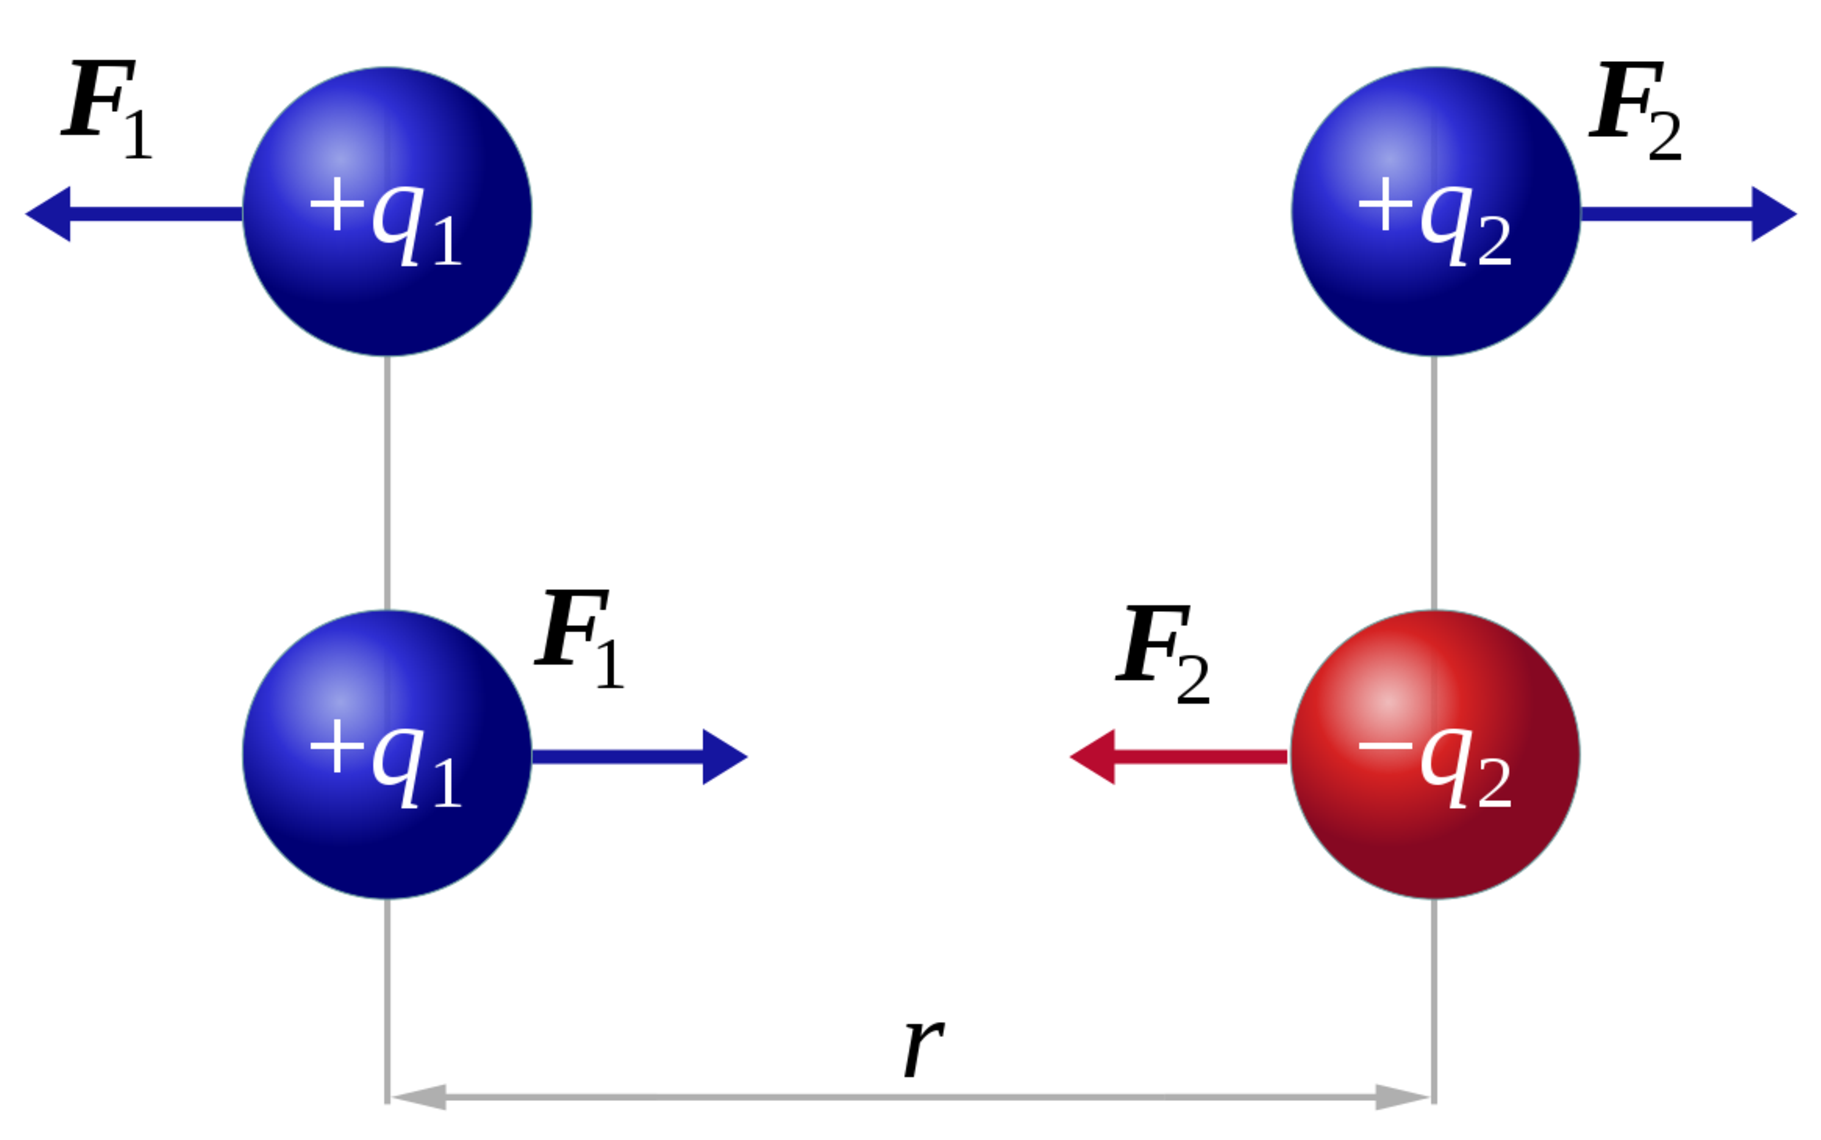
\includegraphics[width=0.5\textwidth]{Elektro/Figurer/Coulomb.eps}
    \caption{Diagram af kræfterne på to ladede partikler når deres ladninger har samme eller modsat fortegn. Kilde: \cite{CoulombLawWikipedia2019}.}
    \label{fig:Coulomb}
\end{figure}

Coulombkraften overholder også princippet om \emph{superposition}: Hvis to ladninger $q_2$ og $q_3$ begge påvirker en ladning $q_1$, så kan den samlede kraft på $q_1$ skrives som en sum, $\va{F}_\text{Total}=\va{F}_{12}+\va{F}_{13}$. Selv for et arbitrært antal ladninger $q_i$, hvor $i=2,3,\dots,N$, der påvirker $q_1$, kan kraften skrives som
\begin{equation} \label{elma:eq:superpos}
    \va{F}=\frac{q_1}{4\pi\varepsilon_0}\sum_{i=2}^{N}\frac{q_i}{\abs{\va{r}_{1i}}^3}\va{r}_{1i} \, .
\end{equation}

Sammenlignet med de kræfter vi typisk arbejder med i mekanik, er Coulombkraften meget speciel på den måde, at den vekselvirker på afstand. F.eks. er friktionskraften og normalkraften kun relevante, når to legemer er i fysisk kontakt. Men Coulombkraften kan skubbe eller tiltrække, om to ladninger er i kontakt, en meter adskilt, eller i modsatte ender af Mælkevejen!
Forestil dig nu følgende hypotetiske scenarie: To ladninger $q_1=\SI{e11}{\coulomb}$ og $q_2=\SI{-e11}{\coulomb}$\footnote{Bemærk at disse ladninger er meget store. Ladningen på én elektron er $\sim\SI{1.6e-19}{\coulomb}$, så det er nærmest umuligt at akkumulere sådan en stor ladning på et sted.}, hver med masse $\SI{1}{\kilogram}$, bliver produceret på samme tid, og placeret præcis et lysår, eller \SI{9.46e15}{\meter}, fra hinanden. Coulombkraften der påvirker de to er så
\begin{equation}
    F=\frac{1}{4\pi\epsilon_0}\frac{\left(\SI{e11}{\coulomb}\right)\times\left(\SI{-e11}{\coulomb}\right)}{\left(\SI{9.46e15}{\meter}\right)^2}=\SI{-1.00}{\newton} \, .
\end{equation}
Hver ladning vil altså føle en tiltrækkende kraft på \SI{1}{\newton} og begynde at accelerere med \SI{1}{\meter\per\second\squared}.

\section{Elektriske felter}
Ovenstående konklusion ledte historisk set til motivationen for, at implementere hvad vi i dag kalder det \emph{elektriske felt}. Et felt skal forstås som noget der eksisterer alle vegne, og der kan sendes signaler igennem dette -- ligesom bølger på en vandoverflade. I feltbeskrivelse tiltrækkes to ladninger via Coulombkraften, fordi feltet fra den ene ladning så at sige fortæller den anden ladningen, at den gerne vil hen imod eller væk fra den første ladning. Ladningen $q_1$ påvirker altså det elektriske felt, som ladningen $q_2$ oplever. Derfra påvirker feltet $q_2$, hvilket resulterer i en tiltrækning eller frastødning. Samme proces sker i modsat retning. Feltet påvirkes af $q_2$, som så påvirker $q_1$. Det elektriske felt er altså et ``medie'', som bliver påvirket af, og som påvirker ladninger.

Det elektriske felt ved en position $\va{r}$, der dannes af ladningen $q$ i punktet $\va r_0$, defineres til at være
\begin{equation} \label{eq:e-felt_punktpartikel}
    \va{E}=\frac{1}{4\pi\varepsilon_0}\frac{q}{\abs{\va r - \va r_0}^3}(\va r - \va r_0) \, .
\end{equation}
Med andre ord, hvis vi vil beregne det elektriske felt fra en ladning $q_1$, som påvirker en anden ladning $q_2$, ligesom på figur \ref{fig:Coulomb}, får vi relationen
\begin{equation} \label{eq:kraft_fra_e-felt}
    \va{E}_{12}=\frac{1}{4\pi\varepsilon_0}\frac{q_1}{\abs{\va r_2 - \va r_1}^3}(\va r_2 - \va r_1)=\frac{\va{F}_{12}}{q_2} \, .
\end{equation}
%
Helt generelt opfylder det elektriske felt, at kraften på en ladning $q$, som resultat af alle elektriske vekselvirkninger er
%
\begin{align} \label{eq:e-felt_def}
    \va F = q\va E \, ,
\end{align}
hvor $\va{E}$ er det totale elektriske felt, der påvirker $q$.

\subsection{Elektriske feltlinjer}

I princippet er vi færdige med elektrostatik, hvilket er studiet af, hvordan ladninger i hvile påvirker hinanden. Ud fra superpositionsprincippet, ligning \eqref{elma:eq:superpos}, kan vi bestemme det elektriske felt af et vilkårligt system af ladninger, og relationen mellem $\va{E}$ og $\va{F}$ fortæller os, hvordan det påvirker andre ladninger.

Meget af det arbejde man vil blive udsat for i elektrostatik ligger dog i at bestemme feltet. Hvad nu hvis feltet ikke var dannet af et endeligt antal punktpartikler med veldefineret ladning, men i stedet var dannet af en kontinuert ladningsfordeling i en given form\footnote{Et eksempel kunne være en skive, hvor skivens overflade har en bestemt mængde ladning per areal.}? Da kan man ikke bruge superpositionsprincippet på formen i ligning \eqref{elma:eq:superpos}, men man må bruge en generaliseret version, som er defineret i form af et integrale i stedet for en sum. Dette gør dog tingene en hel del mere besværlige at arbejde med. Derfor bliver det enormt vigtigt at kunne visualisere og skabe en intuition for de elektriske felter, hvilket kan opnås ved at tegne dets \emph{feltlinjer}. Disse er linjer, der indikerer både retning og styrke af et felt. Retningen af feltet er det samme, som den retning en positiv ladning ville blive skubbet i, hvis den blev placeret i feltet.

Når man tegner de elektriske feltlinjer om en punktladning, kan det repræsenteres som pile, der peger enten ind imod eller ud fra partiklen afhængig af ladningen, som vist på figur \ref{fig:pointcharges}.
\begin{figure}[h!]
    \centering
    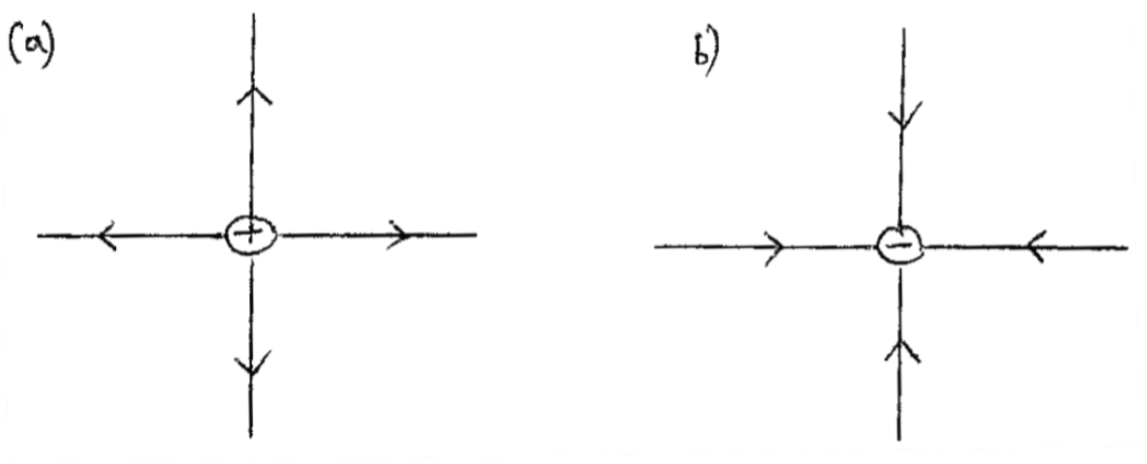
\includegraphics[width=0.8\textwidth]{Elektro/Figurer/fieldline_pointcharges.PNG}
    \caption{Elektriske feltlinjer om en (a) positiv punktladning og en (b) negativ punktladning.}
    \label{fig:pointcharges}
\end{figure}

\noindent Desto flere linjer der er tegnet, jo stærkere er feltet, se figur \ref{fig:pointchargesstrong}. 
\begin{figure}[h!]
    \centering
    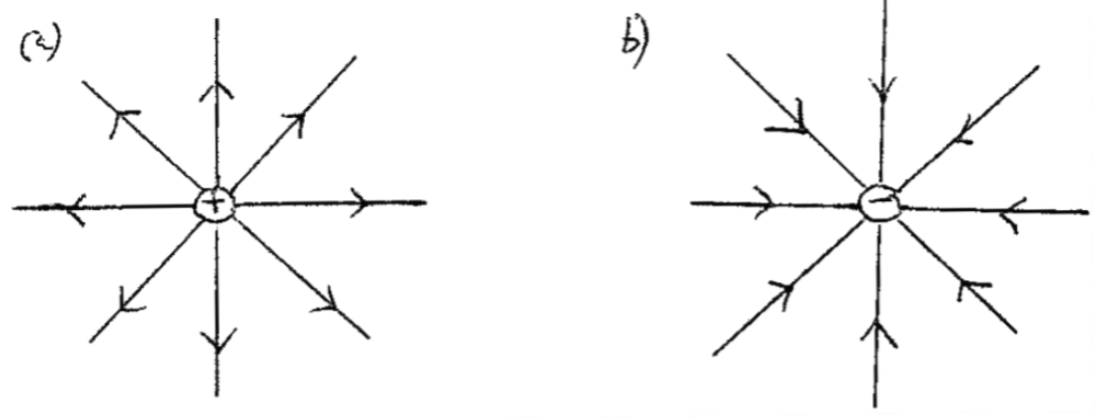
\includegraphics[width=0.8\textwidth]{Elektro/Figurer/fieldline_pointcharges2.PNG}
    \caption{Elektriske feltlinjer om en (a) positiv punktladning og en (b) negativ punktladning med dobbelt så store ladninger som på figur \ref{fig:pointcharges}.}
    \label{fig:pointchargesstrong}
\end{figure}
Som et sidste eksempel kan vi også tegne feltlinjerne for par af punktladninger med enten samme eller forskellig ladning, figur \ref{fig:ElectricFieldLinesTwoCharges}.
\begin{figure}[h!]
    \centering
    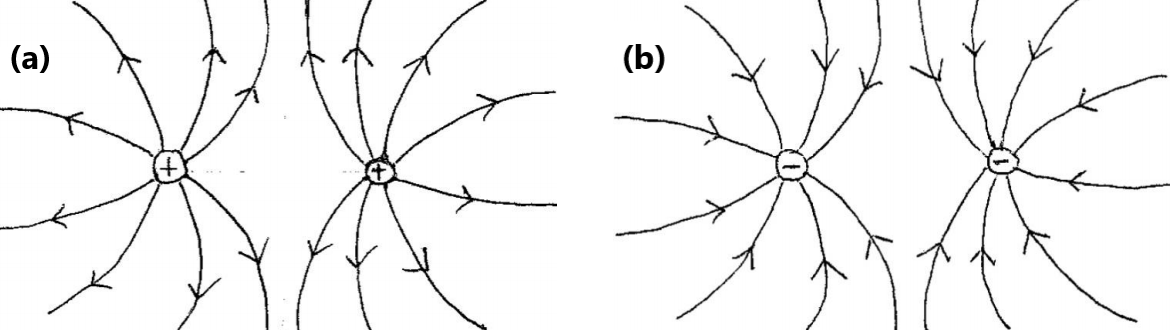
\includegraphics[width=\textwidth]{Elektro/Figurer/fieldline_twocharges.PNG}
    \newline
    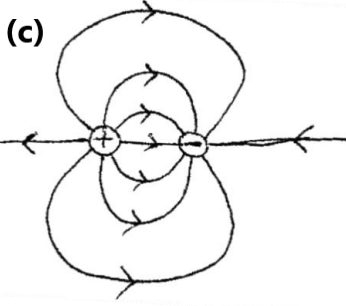
\includegraphics[width=0.37\textwidth]{Elektro/Figurer/fieldline_twocharges2.PNG}
    \caption{Elektriske feltlinjer om par af punktladninger af samme størrelse, (a) for to positive ladninger, (b) to negative ladninger, (c) to modsatte ladninger.}
    \label{fig:ElectricFieldLinesTwoCharges}
\end{figure}
Med disse eksempler i mente, kan vi skrive et sæt regler og yderligere kommentarer om feltlinjer. Nogle stammer fra ren intuition, mens andre følger fra mere avanceret fysik. De er ikke i nogen specifik rækkefølge; det kan endda diskuteres, om de er lige vigtige.
\begin{enumerate}
    \item Feltlinjer eksisterer ikke i virkeligheden. Det er blot en visuel repræsentation som hjælper os med at fortolke fysikken.
    \item Linjernes retning er samme retning som kraften på en positiv ladning i det elektriske felt.
    \item Ovenstående figurer er todimensionelle repræsentationer. I virkeligheden eksisterer felter i 3 dimensioner, men ofte er den todimensionelle repræsentation nok til, at fremhæve den fysik vi er interesserede i.
    \item Feltets tæthed er antallet af feltlinjer per areal (eller volumen i 3D). Feltets tæthed er direkte proportionalt med feltstyrken, så hvis tætheden af feltlinjer fordobles, da vil feltstyrken også fordobles.
    \item Antallet af feltlinjer på en tegning er arbitrær! Hvad der er vigtigt, er den relative tæthed fra et sted til et andet på tegningen.
    \item Hvis der ikke er nogen feltlinje i et område, betyder det at feltstyrken er nul? Ikke nødvendigvis! Det er op til fysikeren, at gøre det nemt at fortolke, hvorhenne feltet faktisk er nul, og hvad der bare er ``mellem linjerne''.
    \item Et eksempel på hvor feltstyrken er nul, er midtpunktet mellem to ladninger af samme størrelse og fortegn. Det er nyttigt at indikere på sit diagram, hvor dette punkt er.
    \item Feltlinjer må aldrig røre hinanden. Dette ville indikere et uendeligt stærkt felt, hvilket ikke er fysisk muligt!
    \item Feltlinjer må aldrig krydse hinanden. Udover en uendelig feltstyrke, ville det betyde forskellige feltretninger i samme punkt.
    \item Elektrostatiske felter starter altid på positive ladninger og slutter på negative.
    \item Feltlinjer viser ikke nødvendigvis den ``sti'', en positiv ladning ville bevæge sig gennem feltet. Det indikerer kun retningen af kraften, ladningen bliver påvirket med.
\end{enumerate}

\section{Elektrisk flux} \label{sec:elektrisk_flux}

I dette og de følgende afsnit vil vi introducere konceptet elektrisk flux, hvilket spiller en stor rolle i elektrostatik. Specielt er den elektriske flux et helt central begreb ift. at formulere Gauss lov, som vi vil kigge på i senere i afsnit \ref{sec:gauss}. Før vi kigger på den præcise definition af elektrisk flux, er det dog værd først at kigge på en sammenhæng mellem feltlinjer og ladning, som vi ikke har dækket endnu.

Vi betragter en kasse, som indeholder en mængde ladning. Da man kan se, at hvis der er tale om en positiv ladning, som på figur \ref{fig:ElectricFluxVisualisation}a,b, vil de elektriske feltlinjer gå ud af kassen. Man siger da, at der er en flux af feltlinjer ud igennem kassens sider. Havde vi i stedet kigget på en negativ ladning, som på figur \ref{fig:ElectricFluxVisualisation}c,d, ville feltlinjerne gå ind i kassen. Man siger da, at der er en flux af feltlinjer ind igennem kassens sider. Ud fra vores viden om elektriske feltlinjer så ved vi, at fordobler vi ladningen, så vil antallet af feltlinjer fra denne ladning også fordobles. Dette er præcis, hvad vi ser fra figur \ref{fig:ElectricFluxVisualisation}a til figur \ref{fig:ElectricFluxVisualisation}b og fra figur \ref{fig:ElectricFluxVisualisation}c til figur \ref{fig:ElectricFluxVisualisation}d.

\begin{figure}[h!]
    \centering
    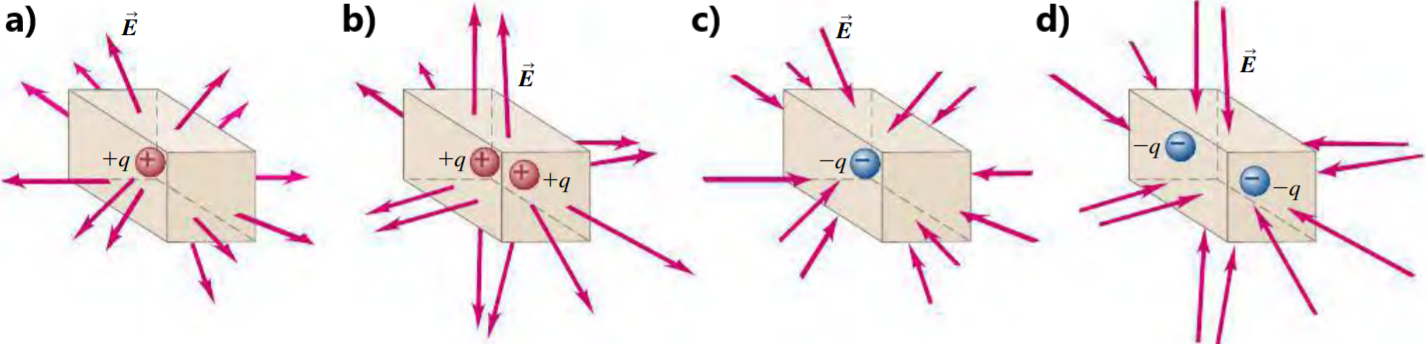
\includegraphics[width=\textwidth]{Elektro/Figurer/ElektricFluxVisualisation.PNG}
    \caption{a) En enkelt positiv ladning i en kasse giver anledning til en udadrettet flux af feltlinjer. b) To positive ladninger giver anledning til dobbelt så stor flux som i (a) gennem den samme kasse, da ladningen er dobbelt så stor. c) En enkelt negativ ladning i en kasse giver anledning til en indadrettet flux af feltlinjer med samme antal feltlinjer som i (a) gennem den sammme kasse. c) To negative ladninger giver anledning til dobbelt så stor flux som i (c) gennem den samme kasse, da ladningen er dobbelt så stor. Kilde: figur 22.2 i \cite{youngSearsZemanskyUniversity2016}.}
    \label{fig:ElectricFluxVisualisation}
\end{figure}

Betragter vi nu den samme kasse, denne gang uden nogen ladning, figur \ref{fig:ElectricFluxVisualisationBoxWithoutCharge}a, så vil der ikke være noget, som kan skabe elektriske feltlinjer, og der vil altså ikke være nogen flux af feltlinjer gennem kassens sider. Indsætter vi i stedet to partikler med ladningerne $q$ og $-q$ i kassen, så vil disse begge skabe elektriske feltlinjer. Det må dog gælde, da de to ladninger har den samme størrelse, at antallet af feltlinjer fra den positive ladning, der vil gå ud igennem kassens sider, er det samme som antallet af feltlinjer fra den negative ladning, der vil gå ind igennem kassens sider, se figur \ref{fig:ElectricFluxVisualisationBoxWithoutCharge}b. Vi kan således konkludere, at den totale flux af feltlinjer gennem kassens sider må være $0$, da feltlinjerne ud og ind af kassen udligner hinanden.  

\begin{figure}[h!]
    \centering
    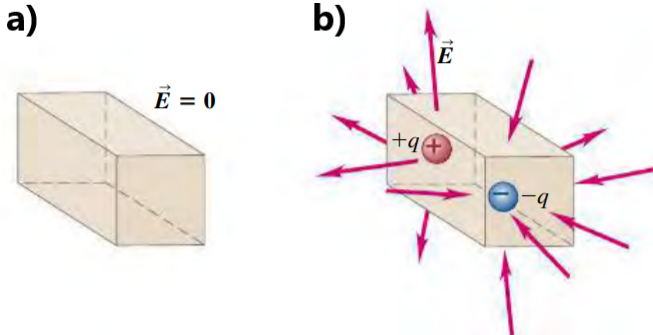
\includegraphics[width=.5\textwidth]{Elektro/Figurer/ElektricFluxVisualisation2.PNG}
    \caption{a) En kasse uden ladning vil ikke have en flux af feltlinjer. b) Den totale ladningen for to partikler med ladningerne $q$ og $-q$ vil være $0$, hvorfor denne konfiguration ikke vil have en flux af feltlinjer. Dette kan også ses af, at fluxen af feltlinjer fra hver af ladningerne udligner hinanden. Kilde: figur 22.3 i \cite{youngSearsZemanskyUniversity2016}.}
    \label{fig:ElectricFluxVisualisationBoxWithoutCharge}
\end{figure}

\subsection{Elektrisk flux i uniformt elektrisk felt}

Ses der først på et uniformt elektrisk felt, altså et elektrisk felt hvor styrken og retningen altid er den samme, så vil den elektriske flux, $\Phi_E$, gennem et areal $A$, der er fladt og står vinkelret på de elektriske feltlinjer, figur \ref{fig:ElectricFlux1}, være givet ved
\begin{align} \label{eq:ElectricFluxUniformFieldFlatPerpendicularArea}
	\Phi_E &= EA \, ,
\end{align}
hvor $E$ er styrken af det elektriske felt, som giver anledning til de elektriske feltlinjer. Heraf kan det ses for uniforme elektriske felter, at den elektriske flux er direkte proportionel med både styrken af det elektriske felt, $E$, samt med størrelsen af arealet, $A$. Det betyder, at hvis arealet øges, så vil den elektriske flux også øges med samme faktor, og ligeså for styrken af feltet.
\begin{figure}[h!]
    \centering
    \begin{subfigure}[t]{.3\textwidth}
        \centering
        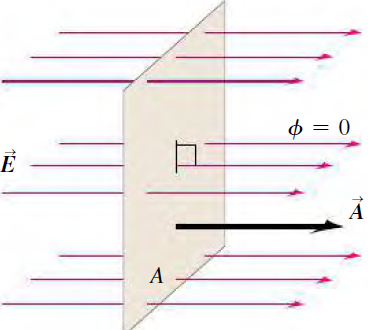
\includegraphics[width=\columnwidth]{Elektro/Figurer/ElectricFlux1.PNG}
        \caption{Overfladen står vinkelret på det elektriske felt, så $\va{E}$ og $\va{A}$ er parallelle (vinklen mellem $\va{E}$ og $\va{A}$ er $\phi = \SI{0}{\degree}$). Fluxen bliver derved $\Phi_E = \va{E} \cdot \va{A} = EA$.}
        \label{fig:ElectricFlux1}
    \end{subfigure}
    \hfill
    \begin{subfigure}[t]{.3\textwidth}
        \centering
        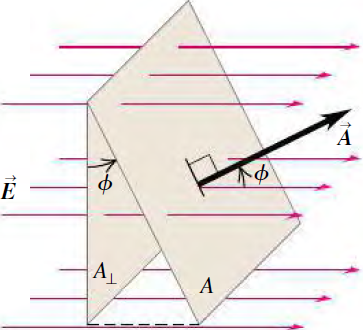
\includegraphics[width=\columnwidth]{Elektro/Figurer/ElectricFlux2.PNG}
        \caption{Overfladen er vinklet med vinklen $\phi$ fra at stå vinkelret på det elektriske felt, så vinklen mellem $\va{E}$ og $\va{A}$ er $\phi$, hvorved fluxen bliver $\Phi_E = \va{E} \cdot \va{A} = EA\cos(\phi)$.}
        \label{fig:ElectricFlux2}
    \end{subfigure}
    \hfill
    \begin{subfigure}[t]{.3\textwidth}
        \centering
        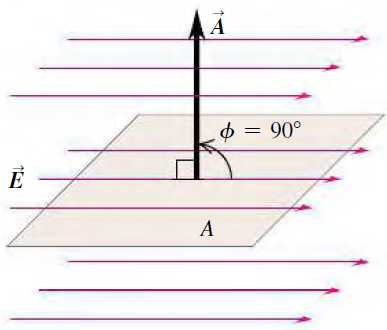
\includegraphics[width=\columnwidth]{Elektro/Figurer/ElectricFlux3.PNG}
        \caption{Overfladen vinklet således, at den er parallel til det elektriske felt, så $\va{E}$ og $\va{A}$ står vinkelret på hinanden (vinklen mellem $\va{E}$ og $\va{A}$ er $\phi = \SI{90}{\degree}$). Fluxen bliver derved $\Phi_E = \va{E} \cdot \va{A} = EA\cos(\SI{90}{\degree}) = 0$.}
        \label{fig:ElectricFlux3}
    \end{subfigure}
    \caption{En flad overflade i et uniformt elektrisk felt. Den elektrisk flux $\Phi_E$ gennem overfladen er givet ved prikproduktet mellem det elektriske felt $\va{E}$ og arealvektoren $\va{A}$. Kilde: figur 22.6 i \cite{youngSearsZemanskyUniversity2016}.}
    \label{fig:ElectricFlux}
\end{figure}

Vinkles dette areal nu således, at det ikke længere står vinkelret på de elektriske feltlinjer, da vil færre af disse passere gennem arealet, idet feltlinjerne kun passerer gennem den del af arealet, $A_\perp$, som står vinkelret på dem, hvilket på figur \ref{fig:ElectricFlux2} og \ref{fig:ElectricFlux3} er svarende til $A_\perp = A\cos(\phi)$ per trigonometri.
Ligning \eqref{eq:ElectricFluxUniformFieldFlatPerpendicularArea} generaliseres derved til
\begin{align} \label{eq:ElectricFluxUniformFieldFlatArea}
	\Phi_E &= EA\cos(\phi) \, .
\end{align}
Dette kan identificeres som værende prikproduktet mellem $\va{E}$ og $\va{A}$ (se evt. ligning \eqref{mat:prikprodukt} ift. prikproduktet)
\begin{align} \label{eq:ElectricFluxUniformFieldFlatAreaScalarProduct}
	\Phi_E &= \va{E} \cdot \va{A} \, ,
\end{align}
hvor $\va{A}$ er \emph{arealvektoren}, hvis retning er repræsenteret ved en enhedsvektor $\vu{n}$ (``normalvektoren''), der står vinkelret på arealet, og hvis længde er lig med størrelsen af arealet, se figur \ref{fig:ElectricFlux}. Vi kan altså arealvektoren som
\begin{align} \label{eq:ElectricFluxAreaVector}
	\va{A} &= A\vu{n} \, .
\end{align}
Idet at en overflade altid har to sider, da vil der være mulighed for to retninger af normalvektoren, og dermed også for arealvektoren, hvorfor dennes retning altid skal specificeres. Ofte betragter vi fluxen, hvilken f.eks. kan stamme fra en punktladning, ud gennem et lukket overflade, og i disse tilfælde vælger vi per konvention normalvektorens retning til at være udad fra overfladen. Det vil dermed være retningen af det elektriske felt, der bestemmer om den elektriske flux er positiv eller negativ. Fra ligning \eqref{eq:ElectricFluxUniformFieldFlatAreaScalarProduct} kan man se, at $\Phi_E>0$, når det elektriske felt peger ud igennem den lukkede overflade, da vinklen $\phi$ mellem feltet og arealvektoren her vil opfylde at: $0\degree < \phi < 90\degree$. Modsat vil man have, at $\Phi_E < 0$, når det elektriske felt peger ind igennem den lukkede overflade, hvilket følger af et lignede argument som ovenfor.

\subsection{Generalisering af elektrisk flux}

I foregående afsnit blev der fundet en beskrivelse af den elektriske flux for et uniformt elektrisk felt gennem en flad overflade, men dette er ikke altid tilfældet. Man kan forestille sig, at det elektriske felt ikke er uniformt, altså at det ændrer sig alt efter ens rummelige placering, eller at overfladen, som man regner fluxen gennem, er krum, som f.eks. en kugleskal, hvilket vi endnu ikke har taget højde for. Vi vil derfor generalisere udtrykket for den elektriske flux fundet i ligning \eqref{eq:ElectricFluxUniformFieldFlatAreaScalarProduct}.

Til dette formål opdeler vi dermed overfladen i mange små dele $\dd{A}$, som hver har sin egen normalvektor $\vu{n}$ vinkelret på dem, har en arealvektor $\dd{\va{A}} = \dd{A}\vu{n}$, og kan ses som værende i et uniformt elektriske felt\footnote{Ethvert elektrisk felt vil være uniformt, hvis man kigger på det indefor en tilpas lille volumen. Dette er lidt det samme, som at jorden for os opleves som værende flad, selvom den jo i det store billede er rund.}. Den elektriske flux gennem hvert af disse arealer beregnes ved ligning \eqref{eq:ElectricFluxUniformFieldFlatAreaScalarProduct}, og resultaterne integreres op (husk at integraler en form for ``sum'') for at finde den totale elektriske flux
\begin{align} \label{eq:ElectricFlux}
	\Phi_E &= \int_S \va{E} \cdot \dd{\va{A}} \, .
\end{align}
Integralet i ligning \eqref{eq:ElectricFlux} er et overfladeintegral (dobbeltintegral), hvor $S$ angiver den overflade, som man integrerer over.

\subsubsection{Elektrisk flux gennem en cirkulær overflade}

\begin{figure}[t]
    \centering
    \begin{subfigure}[t]{.45\textwidth}
        \centering
        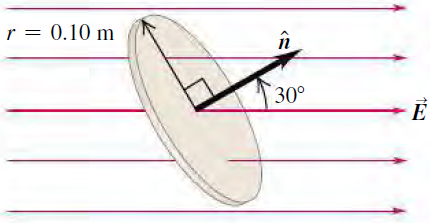
\includegraphics[width=\columnwidth]{Elektro/Figurer/ElectricFluxThroughADisk.PNG}
        \caption{En circulær disk med radius $R = \SI{0.10}{\meter}$ er placeret i et uniformt elektrisk felt $\va{E}$, så dens normalvektor $\vu{n}$ er i en vinkel af $\phi = \SI{30}{\degree}$ til det elektriske felt. Kilde: figur 22.7 i \cite{youngSearsZemanskyUniversity2016}.}
        \label{fig:ElectricFluxThrougADisk}
    \end{subfigure}
    \hfill
    \begin{subfigure}[t]{.45\textwidth}
        \centering
        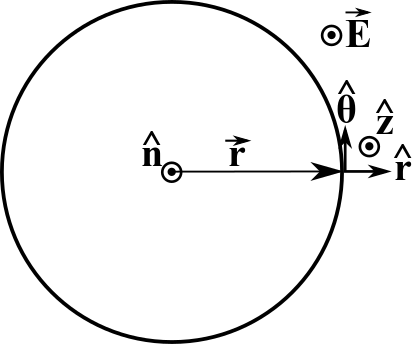
\includegraphics[width=.65\columnwidth]{Elektro/Figurer/ElectricFluxExercise.png}
        \caption{Den samme cirkulære disk placeres nu i et ikke uniformt elektrisk felt $\va{E} = E_0 r \vu{z}$ i samme retning som det foregående, hvor $E_0 = \SI{2.0e3}{\newton/\coulomb}$, og disken rettes nu op således, at den står vinkelret på feltet ($\phi = 0$).}
        \label{fig:ElectricFluxThrougADisk2}
    \end{subfigure}
    \caption{En cirkulær disk med radius $R = \SI{0.10}{\meter}$ placeres i et elektrisk felt $\va{E}$.}
    \label{fig:ElectrixFluxExample}
\end{figure}

Som eksempel kan vi se på en rund disk placeret i et uniformt elektrisk felt $\va{E}$ med størrelsen $\SI{2.0e3}{\newton/\coulomb}$. Disken har en radius på $R = \SI{0.10}{\meter}$ og er vinklet i forhold til det elektriske felt med vinklen $\phi = \SI{30}{\degree}$. Diskens normalvektor er orienteret som set på figur \ref{fig:ElectricFluxThrougADisk}, hvilket er nødvendigt at specificere, da en disk ikke er en lukket overflade og dermed ikke har en inderside og en yderside. Vi ønsker nu at finde den elektriske flux gennem disken.

Idet disken er placeret i et uniformt elektrisk felt benytter vi ligning \eqref{eq:ElectricFluxUniformFieldFlatAreaScalarProduct}
\begin{align}
    \Phi_E &= \va{E} \cdot \va{A} \, .
\end{align}
Vi skal altså kende det elektriske felt $\va{E}$ og arealvektoren $\va{A}$. Styrken af det elektriske felt er som nævnt givet til at være $E = \SI{2.0e3}{\newton/\coulomb}$. Arealvektoren findes ved ligning \eqref{eq:ElectricFluxAreaVector} som arealet af disken ganget med normalvektoren $\vu{n}$, så $\va{A} = A\vu{n}$, hvor $A = \pi R^2$. Vinklen mellem det elektriske felt $\va{E}$ og arealvektoren $\va{A}$ er $\phi = \SI{30}{\degree}$, så vi får fluxen gennem disken til at være
\begin{align}
    \Phi_E &= EA\cos(\phi)
        = E \pi R^2 \cos(\phi)
        = \left(\SI{2.0e3}{\frac{\newton}{\coulomb}}\right) \left(\SI{0.0314}{\meter^2}\right) \cos\left(\SI{30}{\degree}\right)
        = \SI{54}{\frac{\newton\meter^2}{\coulomb}} \, .
\end{align}
Placeres den samme disk nu i et ikke uniformt elektrisk felt, $\va{E} = E_0 r \vu{z}$, hvor $E_0 = \SI{2.0e3}{\newton/\coulomb}$, som set på figur \ref{fig:ElectricFluxThrougADisk2}, kan ligning \eqref{eq:ElectricFluxUniformFieldFlatAreaScalarProduct} ikke længere bruges til at beregne fluxen, men man skal i stedet benytte ligning \eqref{eq:ElectricFlux}. Idet at det elektriske felt kun afhænger af afstanden til centrum, $r$, og da disken er symmetrisk omkring origo (centrum af disken), kan man skrive arealetelementet $\dd{A}$ ved brug af ligning \eqref{eq:ArealElementMat}. Det giver at
\begin{align}
    \dd{\va{A}} &= 2\pi r \dd{r} \vu{n} = 2\pi r \dd{r} \zhat \, ,
\end{align}
hvor det er brugt, at $\vu{n} = \zhat$ her, som det fremgår af figur \ref{fig:ElectricFluxThrougADisk2}. Fluxen gennem hele disken findes dermed vha. \eqref{mat:eq:polardoubleint}, hvilket giver
\begin{align} \label{eq:ElectricFluxExampleStep1}
	\Phi_E &= \int_S \va{E} \cdot \dd{\va{A}}
	    = \int_{0}^{R} \left(E_0 r \vu{z}\right) \cdot \left(2\pi r \dd{r} \zhat \right)
	    = 2\pi E_0 \int_{0}^{R} r^2 \left(\zhat \cdot \zhat)\right \dd{r}
	    = 2\pi E_0 \int_{0}^{R} r^2 \dd{r} \, ,
\end{align}
hvor det er benyttet, at $\zhat \cdot \zhat = 1$, og at man må sætte konstanter udenfor integralet. Udregnes dette integral fås
\begin{align} \label{eq:ElectricFluxExampleStep2}
	\Phi_E &= 2\pi E_0 \int_{0}^{R} r^2 \dd{r}
	    = 2\pi E_0 \left[\frac{1}{3}r^3\right]_{0}^{R}
	    = \frac{2}{3}\pi E_0 \left[ r^3\right]_{0}^{R}
	    = \frac{2}{3} \pi E_0 R^3 \, ,
\end{align}
hvor leddet tilhørende den nedre grænse er droppet, da det giver nul her. Indsættes den givne værdi for det elektriske felts styrke $E_0 = \SI{2.0e3}{\newton/\coulomb}$ samt diskens radius $R = \SI{0.10}{\meter}$ fås fluxen gennen disken til at være
\begin{align}
    \Phi_E &= \frac{2}{3} \pi \cdot \SI{2.0e3}{\frac{\newton}{\coulomb}} \cdot (\SI{0.10}{\meter})^3
	    = \SI{4.2}{\frac{\newton\meter^2}{\coulomb}} \, .
\end{align}


\subsection{Gauss' lov} \label{sec:gauss}
Gauss' lov er en måde at beskrive forholdet mellem elektriske ladninger og felter. Loven fortæller, at den elektriske flux gennem en lukket overflade, som indelukker et endeligt volumen, er proportional med den totale elektriske ladning indenfor overfladen.

Dette kan vi vise ved først at kigge på en enkelt positivt ladet partikel med ladning $q$. Denne ladningen placeres i centrum af en imaginær sfære med radius $R$, hvor vi så vil regne fluxen gennem denne sfæres overflade. Fra ligning \eqref{eq:e-felt_punktpartikel} vides det, at det elektriske felt fra ladningen er
\begin{align}
    \va{E} = \frac{1}{4\pi\epsilon_0} \frac{q}{\abs{\va{r}}^3} \va{r} \, ,
\end{align}
da udgangspunktet $\va{r}_0$ her er i sfærens centrum, så $\va{r}_0$ er nulvektoren her. Ved ethvert punkt på overfladen af sfæren vil det elektriske felt (som peger udad) være vinkelret til overfladen, da feltlinjerne fra ladning udsendes ligeligt i alle retninger, som på figur \ref{fig:pointchargesstrong}. Da må styrken af det elektriske felt, $E$, her  kun afhænger af afstanden til centrum, $r$, må feltet altså have samme styrke på hele sfærens overfalde. Derved bliver den totale elektriske flux blot produktet af det elektriske felts styrke på overfladen af sfæren (radius $R$) og overfladearealet af sfæren selv $A$. Altså får man at
\begin{align} \label{eq:GaussLawSphere}
    \Phi_E &= EA = \frac{1}{4\pi\epsilon_0} \frac{q}{R^2} (4 \pi R^2) = \frac{q}{\epsilon_0} \, .
\end{align}
Fluxen er derved uafhængig af sfærens radius og afhænger kun af den indesluttede ladning $q$. Bemærk specielt at fluxen som påstået er proportional med den indesluttede ladning $q$ med $1/\epsilon_0$ som proportionalitetskonstant. 

\begin{figure}[h!]
    \centering
    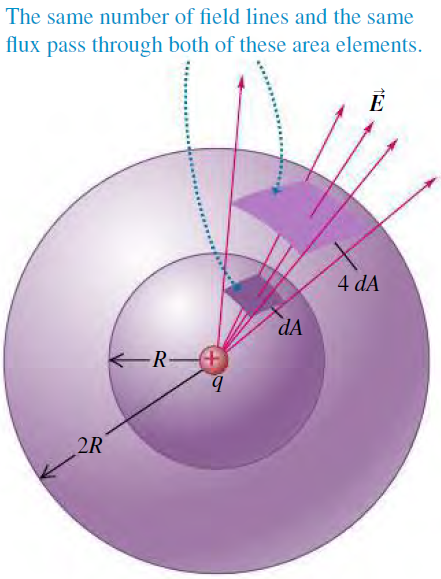
\includegraphics[width=.4\textwidth]{Elektro/Figurer/GaussLawProjectingOntoASphere.PNG}
    \caption{Projektion af et lille areal $\dd{A}$ fra overfladen af en sfære med radius $R$ på overfladen af en sfære med radius $2R$. Kilde: figur 22.11 i \cite{youngSearsZemanskyUniversity2016}.}
    \label{fig:GaussLawProjectingOntoASphere}
\end{figure}

Uafhængiheden af sfærens radius kan også ses, hvis vi kigger på en lille del af overfladen, arealelementet $\dd{A}$, på sfæren med radius $R$. Projiceres\footnote{Delen af arealet projiceres ved at trække linjer fra ladningen i centrum gennem hjørnerne af arealdelen i afstanden $R$ og ende i afstanden $2R$, hvor slutpunkterne kan forbindes til af vise arealet projiceret på sfæren med radius $2R$.} denne på en sfære med radius $2R$, figur \ref{fig:GaussLawProjectingOntoASphere}, så arealet på sfæren med radius $2R$ bliver $4\dd{A}$, da hver side af arealelementet bliver dobbelt så stor. Men siden det elektriske felt er omvendt proportionalt med afstanden kvadreret ($E \propto 1/r^2$) vil størrelsen af dette være $4$ gange mindre i afstanden $2R$ fra centrum, hvorfor disse frontfaktorer ($4$ og $1/4$) vil gå ud, når fluxen beregnes. Altså vil fluxen gennem de to arealer være ens uafhængigt af de pågældende sfærers radius.

\begin{figure}[h!]
    \centering
    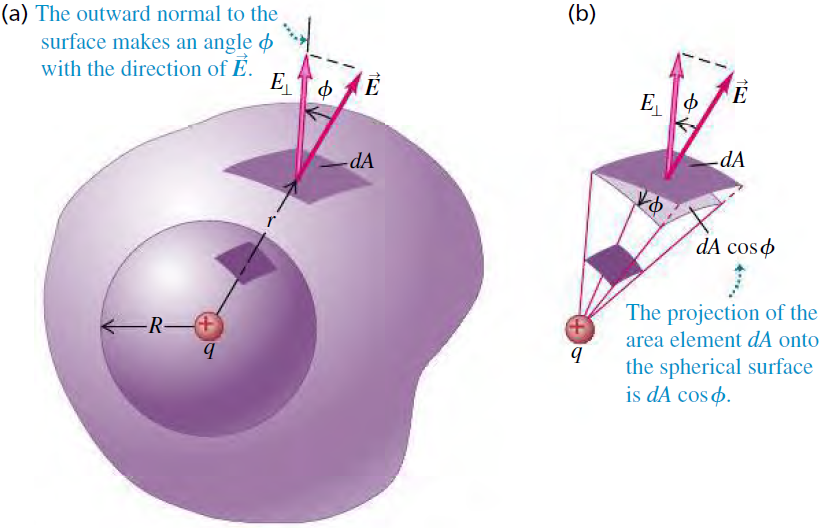
\includegraphics[width=.75\textwidth]{Elektro/Figurer/GaussLawProjectingOntoAnArbitraryShape.PNG}
    \caption{Projektion af et lille areal $\dd{A}$ fra overfladen af en sfære med radius $R$ på overfladen af en ikkesfærisk overflade i afstanden $r$. Kilde: figur 22.12 i \cite{youngSearsZemanskyUniversity2016}.}
    \label{fig:GaussLawProjectingOntoanArbitraryShape}
\end{figure}

For at generalisere Gauss' lov til ikke-sfæriske overflader benyttes projiceringsteknikken igen, men i stedet for en ydre sfære er den indre sfære af radius $R$ omgivet af en irregulær overflade, som på figur \ref{fig:GaussLawProjectingOntoanArbitraryShape}a. Tager vi et lille arealelement $\dd{A}$ på den irregulære overflade i en afstand $r$ til ladningen og projicerer dette ned på en kugleskal i samme afstand, så vil to af siderne, som set på figur \ref{fig:GaussLawProjectingOntoanArbitraryShape}b, blive forkortet med $\cos(\phi)$, hvor $\phi$ er vinklen mellem arealelementets normal $\vu{n}$ og det elektriske felt $\va{E}$. De to resterende sider af arealelementet forbliver uændrede, hvorved det projicerede arealelement er givet ved $\dd{A}\cos(\phi)$. Analogt til at projicere arealelementet, der ikke er vinkelret på det elektriske felt, ned på sfæren, hvor elementet er vinkelret på feltet, da kan man i stedet projicere det elektriske felt, der ikke er vinkelret på arealelementet, på normalvektoren for arealelementet, så denne projektion $E\cos(\phi)$ vil være vinkelret på arealelementet. Dette skyldes, at man uanset hvad får retningen af arealvektoren og det elektriske felt til at være parallelle efter projektion af den ene af dem, hvorved man for at finde fluxen blot multiplicerer den ene med den anden, hvorfor det er irrelevant, om $\cos(\phi)$ er ganget på den ene eller den anden parameter. Den elektriske flux gennem det valgte arealelement bliver derved $E\dd{A}\cos(\phi)$.

Opdeles hele den irregulære overflade i små arealelementer kan fluxen gennem hvert af disse regnes som ovenstående og summeres ved integration over hele overfladen. Den totale elektrisk flux gennem den irregulære overflade, givet ved ligning \eqref{eq:ElectricFlux}, skal være den samme som den totale flux gennem en sfære, som set ovenfor, hvilket per ligning \eqref{eq:GaussLawSphere} er lig $q/\epsilon_0$. Derfor vil den totale flux gennem den irregulære overflade være
\begin{align} \label{eq:GaussLawArbitraryShape}
    \Phi_E &= \oint_S \va{E} \cdot \dd{\va{A}} = \frac{q}{\epsilon_0} \: .
\end{align}
Dette er Gauss' lov, hvilken holder for enhver lukket overflade, der indeslutter en ladning $q$. Cirklen på integralet betyder, at integralet altid skal beregnes over en lukket overflade.

I ovenstående udledning var blot placeret en enkelt ladning $q$ indenfor den irregulære overflade, men Gauss' lov kan generaliseres til at indeholde et vilkårligt antal ladninger
\begin{align} \label{eq:GaussLawGeneral}
    \oint_S \va{E} \cdot \dd{\va{A}} &= \frac{Q_{\text{inde}}}{\epsilon_0} \: ,
\end{align}
hvor $Q_{\text{inde}}$ er den totale ladning indesluttes af overfladen, og $\va{E}$ er det totale elektriske felt beregnet ved superpositionsprincippet.

%
\begin{figure}
    \centering
    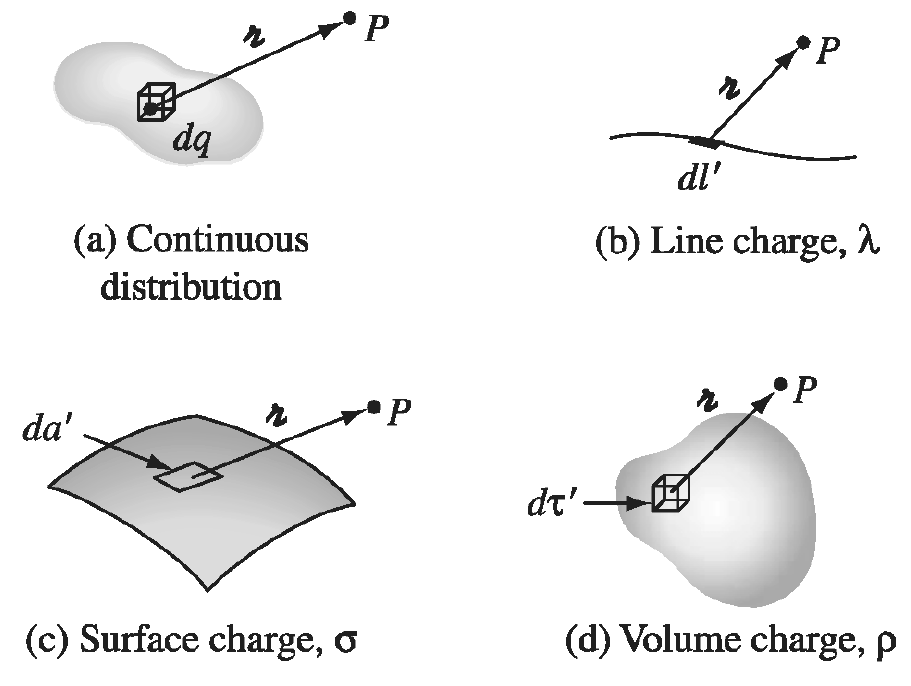
\includegraphics[width=.6\columnwidth]{Elektro/Figurer/ladningsfordeling.PNG}
    \caption{Illustration af kontinuerte ladningsfordelinger i 1, 2 og 3 dimensioner. Det vigtige i figuren er illustrationerne og ikke det vektorer og parametre, der er indtegnet i figuren. Kilde: figur 2.5 i \cite{griffithsIntroductionElectrodynamics2017}.}
    \label{fig:ladningsfordeling}
\end{figure}
%
\subsubsection{Ladningsfordeling}
Så længe et system har en symmetri, der gør det muligt at løse integralet i ligning \eqref{eq:GaussLawGeneral} kan Gauss' lov bruges til at bestemme det elektriske felt overalt i rummet. For at gøre det skal den indesluttede ladning bestemmes. Til at beskrive hvordan ladningen er fordelt i rummet bruges en kontinuert\footnote{For de matematisk interesserede så sikrer kontinuitetskravet at ladningstæthedsfunktionerne er integrable, se side 366 i \cite{stewartCalculusConceptsContexts2006}, således at deres integraler kan bruges til at bestemme mængden af ladning i et område.} \textit{ladningstæthedsfunktion}. At ladningsfordelingen er kontinuert betyder at vi betragter ladning som værende smurt ud i rummet i stedet for at være samlet i diskrete punkter. Ladningstæthedsfunktioner opdeles i tre tilfælde efter hvor mange dimensioner ladningen er fordelt i med hver deres symbol:
%
\begin{itemize}
    \item Lineær ladningstæthed, $\lambda$
    \item Overfladeladningstæthed, $\sigma$
    \item Volumenladningstæthed, $\rho$
\end{itemize}
%
Figur \ref{fig:ladningsfordeling} viser illustrationer af de forskellige typer ladningstætheder. Hvis alt ladningen er samlet på en linje i rummet, så beskrives den ved den lineære ladningstæthed, $\lambda$, uanset hvor krøllet og mystisk denne linje er. Tilsvarende beskriver overfladeladningstætheder, $\sigma$, alt hvad der kan beskrives i to dimensioner, men ikke i én dimension, og i det sidste tilfælde hvor ladningen er fordelt i alle tre rummelige dimensioner bruges volumenladningstætheden, $\rho$. En tæthedsfunktion har den egenskab at dens integral giver mængden af hvad den beskriver indenfor et bestemt område i rummet. På lidt mere almindeligt dansk, så findes ladningen på en linje fra punktet $a$ til punktet $b$, som kaldes $Q_{ab}$, ved at integrere den lineære ladningstæthedsfunktion, $\lambda$:
%
\begin{subequations} \label{eq:ladningsfordeling}
    \begin{align} \label{eq:line_charge}
        Q_{ab} = \int_a^b \lambda \dd{l}.
    \end{align}
    %
    Her er integrationsvariablen $l$, da det gælder generelt for alle linjer. Hvis linjen er ret og i $x$-aksen, så ville integrationsvariablen være $x$. Hvis der er tale om en overfladeladningstæthed, så skal man integrere i to dimensioner. Ladningen i en plan parallelt med $xy$-planen indenfor et rektangel udspændt af punkterne $(x_1,y_1),(x_2,y_1),(x_1,y_2),(x_2,y_2)$ er så
    %
    \begin{align}
        Q = \int \sigma \dd{A} = \int_{x_1}^{x_2}\int_{y_1}^{y_2} \sigma \dd{x}\dd{y}.
    \end{align}
    %
    Er der slutteligt tale om en volumenladningstæthed er der tale om et rummeligt integral
    %
    \begin{align} \label{eq:volumenladning}
        Q = \int \rho \dd{V}.
    \end{align}
\end{subequations}
%
Ofte kan integralerne forsimples ved brug af symmetriargumenter. Et vigtigt specialtilfælde af ligning \eqref{eq:ladningsfordeling} er den uniforme ladningsfordeling. Uniform betyder ensartet eller med andre ord konstant og af ligning \eqref{mat:eq:konstant} fremgår det at konstanter kan trækkes udenfor integralet og således giver ligning \eqref{eq:line_charge}
%
\begin{align}
    Q_{ab} = \int_a^b \lambda \dd{l} = \lambda \int_a^b \dd{l} = \lambda(b-a).
\end{align}
%
At løse disse integraler kan være lidt en kunst og derfor holder vi os her til nogle af de simpleste tilfælde og hjælpe læseren til en introduktion til denne gren af fysikken\footnote{For den interesserede læser så giver \cite{youngSearsZemanskyUniversity2016} en mere uddybende introduktion til emnet, mens \cite{griffithsIntroductionElectrodynamics2017} giver en grundig gennemgang af hele elektrodynamikken.}.

\subsubsection{To uendelig lange ladede cylindere} \label{sec:gauss_lov_eksempel}
Som eksempel på brugen af Gauss' lov kan vi se på to uendelig lange, koaksiale\footnote{De to cylindres ligger begge med centrum langs $\vu{z}$-aksen.} ladede cylindre, hvor den inderste (mørk grå) er en ikkehul cylinder med en uniform volumenladningstæthed $\rho$, mens den ydre (lys grå) er hul og har en uniform overfladeladningstæthed på $\sigma$. Denne opstilling kan ses på figur \ref{fig:GaussLawExample}a. Vi ønsker at bestemme det elektriske felt tre forskellige steder i forhold til cylindrene: Indeni den inderste cylinder (\textcolor{green}{grøn} stiplet linje), mellem den inderste og den yderste cylinder (\textcolor{blue}{blå} stiplet linje) og udenfor den yderste cylinder (\textcolor{red}{rød} stiplet line). For at beregne det elektriske felt disse tre steder indlægges hver sted (altså med radier $r < r_1$, $r_1 < r < r_2$ og $r > r_2$) en Gauss overflade, der her er en Gauss cylinder, da der er cylindrisk symmetri, hvilket skyldes, at det elektriske felt vil blive udsendt i den radiære\footnote{Den radiære retning er langs retningen af $\va{r}$-vektoren. I cylindrisk symmetri vil dette være fra centrum af cylinderen og ud gennem dens sidevægge.} retning $\va{E} = E\vu{r}$. Det bemærkes, at grundet den cylindriske symmetri vil det elektriske felt $\va{E}$ være parallelt med arealvektoren $\dd{\va{A}}$, hvorfor $\va{E} \cdot \dd{\va{A}} = E\dd{A}$. Vi kigger nu på de tre Gauss overflader:

\begin{figure}[t]
    \centering
    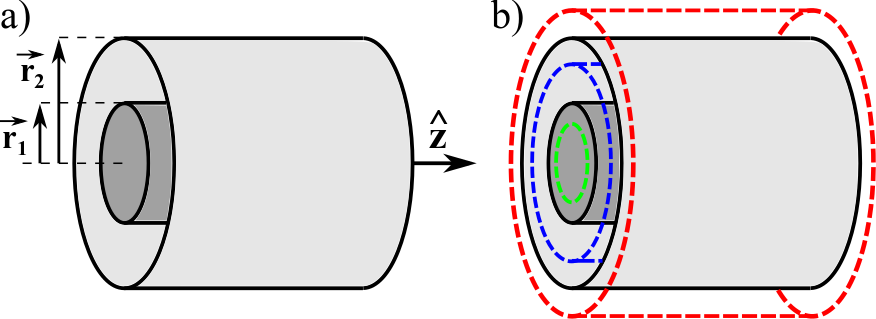
\includegraphics[width=\textwidth]{Elektro/Figurer/GaussLawExample.png}
    \caption{a) En ikkehul cylinder (mørk grå) med radius $r_1$ og uniform volumenladningstæthed $\rho$ per længdeenhed er placeret koaksialt i en hul cylinder (lys grå) med radius $r_2$ og uniform overfladeladningtæthed $\sigma$. Begge cylindre antages at være uendelig lange, således at problemet er cylindrisk symmetrisk over alt. b) Tre Gausscylindre er placeret koaksialt med de to uendeligt lange ladede cylindre: Én indenfor den inderste cylinder, én mellem de to cylindre kun indkapslende den inderste cylinder, og en indkapslende begge cylindre.}
    \label{fig:GaussLawExample}
\end{figure}

\begin{itemize}
    \item $\mathbf{r < r_1}$\textbf{:} Ladningen inden i den inderste cylinder er uniformt fordelt, hvorfor udtrykket for den indesluttede ladning vil være afhængig af cylinderens volumen
    \begin{align}
        Q_{\text{inde}}(r) &= \rho\pi r^2 z \: ,
    \end{align}
    hvor $z$ her angiver en længdeenhed.
    Ved at gøre brug af Gauss' lov (ligning \eqref{eq:GaussLawGeneral}) fås derved
    \begin{align}
        \frac{Q_{\text{inde}}}{\epsilon_0} &= \frac{\rho\pi r^2 z}{\epsilon_0}
            = \oint_S \va{E} \cdot \dd{\va{A}}
            = \oint_S E \dd{A}
            = E \oint_S \dd{A} \: .
    \end{align}
    Idet arealet af en cylinder er givet som produktet af omkredsen af en cirkel og længden af cylinderen fås
    \begin{align}
        \frac{\rho\pi r^2 z}{\epsilon_0} &= E \cdot 2\pi r z \: ,
    \end{align}
    så størrelsen af det elektriske felt indeni den inderste cylinder er
    \begin{align}
        E(r) &= \frac{\rho\pi r^2 z}{2\pi\epsilon_0 r z}
            = \frac{\rho}{2\epsilon_0}r
    \end{align}
    \item $\mathbf{r_1 < r < r_1}$\textbf{:} For Gauss cylinderen, der er placeret imellem de to cylindre, er den indesluttede ladning per længdeenhed ladningen per længdeenhed af den inderste cylinder multipliceret med dennes overfladeareal, $Q_{\text{inde}} = \rho \pi r_1^2 z$. Ved benyttelse af samme metode som ovenfor fås størrelsen af det elektriske felt til
    \begin{align}
        \frac{\rho \pi r_1^2 z}{\epsilon_0} &= E \oint_S \dd{A}
            = E \cdot 2\pi r z \\
        \Rightarrow E(r) &= \frac{\rho}{2\epsilon_0}\frac{r_1^2}{r} \: .
    \end{align}
    \item $\mathbf{r > r_2}$\textbf{:} For en Gauss cylinder udenfor den yderste af cylindrene er den indesluttede ladning per længdeenhed den samlede ladning per længdeenhed af den inderste og den yderste cylinder multipliceret med længden af Gauss cylinderen, $Q_{\text{inde}} = \rho \pi r_1^2 z + 2 \sigma \pi r_2 z$. Ved at benytte samme metode som ovenfor fås størrelsen af det elektriske felt til
    \begin{align}
        \frac{\pi z \left(\rho r_1^2 + 2 \sigma r_2 \right)}{\epsilon_0} &= E \oint_S \dd{A}
            = E \cdot 2\pi r z \\
        \Rightarrow E(r) &= \frac{1}{2\epsilon_0 r}\left(\rho r_1^2 + 2\sigma r_2\right) \: .
    \end{align}
\end{itemize}




\section{Magnetiske felter}
Med Gauss' lov bliver elektriske felter i situationer med tilstrækkelig symmetri markant lettere at bestemme, men metoden til at bestemme disse felter, er begrænset til det der hedder elektrostatiske situationer. Det betyder at ladningerne, der skaber feltet, står stille. Der er ikke fordi Gauss' lov kun gælder for stillestående ladninger, men snarere at ladningernes bevægelse ændrer på symmetrien, således at det ophører at være en smart måde at gøre tingene på. Til dette formål introduceres det magnetiske felt, der udfylder den samme rolle for ladninger i bevægelse, som elektriske felter gør for stillestående ladninger. Ligning \eqref{eq:e-felt_punktpartikel} definerer det elektriske felt fra en stillestående ladning. Placeres en punktladning, $q$, i punktet $\va r_0$, med hastigheden $v$ så defineres det magnetiske felt i punktet $\va r$ som
%
\begin{align} \label{eq:b-felt_fra_punktladning}
    \va B(\va r) = \frac{\mu_0}{4\pi}\frac{q\va v \times (\va r - \va r_0)}{|\va r - \va r_0|^3}.
\end{align}
%
Her er $\mu_0$ vakuumpermeabilitet, der fortæller hvor kraftigt en ladning bliver påvirket af et magnetfelt i vakuum, ligesom $\epsilon_0$ gør for elektriske felter i vakuum. $4\pi$ er en geometrisk faktor, som kommer fra at vi lever i 3 dimensioner, præcis ligesom i Coulombs lov. Placeres en anden ladning, $Q$, i punktet $\va r$ med hastigheden $\va v'$, så er den magnetiske kraft på denne ladning fra magnetfeltet i ligning \eqref{eq:b-felt_fra_punktladning}
%
\begin{align} \label{eq:magnetisk_kraft}
    \va F_{mag} = Q\va v' \times \va B(\va r).
\end{align}
%
En vigtig ting, der nu kan ses, er at fortolkningen af elektriske og magnetiske felter er forskellige. Om elektriske felter gælder det at $\va F \propto \va E$, nemlig at kraften fra et elektrisk felt på en ladning peger i samme retning som det elektriske felt. I kapitel \ref{sec:vektorer} blev krydsproduktet introduceret, og det blev bemærket at krydsproduktet står vinkelret på de to vektorer, der er `ganget' sammen. Det betyder at kraften på en ladning fra et magnetisk felt står vinkelret på både det magnetiske felt, men også den retning som ladningen bevæger sig i, samt at stillestående ladninger ikke er påvirket af magnetfelter.

\subsection{Ladning i uniformt magnetfelt} \label{sec:uniformt_b-felt}
For at få en føling med retningen på den magnetiske kraft, undersøges hvordan et uniformt magnetfelt påvirker en ladning i bevægelse. At magnetfeltet er uniform betyder at det er ens alle steder i rummet. Mere specifikt kiggest på det magnetiske felt $\va B = B_0 \zhat$, hvilket betyder at feltet peger i $z$-retningen og har størrelsen $B_0$. En ladning $q$ med hastigheden $\va v = v_y \yhat$ bliver påvirket af dette magnetfelt. For at kunne bruge ligning \eqref{eq:magnetisk_kraft} til at bestemme den magnetiske kraft, skal krydsproduktet mellem $\va v$ og $\va B$ bestemmes, hvilket er en oplagt mulighed til at få lidt træning i at regne disse. Først huskes på definitionen af enhedsvektorerne, hvorefter \ref{eq:krydsprodukt} kan bruges til at få
%
\begin{align}
    \yhat \times \zhat = \xyz{0}{1}{0} \times \xyz{0}{0}{1} = \xyz{1}{0}{0} = \xhat.
\end{align}
%
Nu kan ligning \eqref{eq:magnetisk_kraft} bruges til at få
%
\begin{align}
    \va F = q\va v \times \va B = qv_y\yhat \times B_0 \zhat = qv_yB_0\yhat \times \zhat = qv_yB_0\xhat.
\end{align}

\subsection{Strøm}
Inden beskrivelsen af magnetiske felter kan fortsætte, skal begrebet strøm introduceres fysisk. I daglig tale så er strøm sådan noget, der løber i ledninger og sørger for at elektriske apparater har energi til hvad end de laver. I fysik er en strøm en gruppe ladninger, der bevæger sig samlet set på en ordnet måde. I praksis er det meget det samme, som den dagligdags forståelse. Fysisk ville man sige at elektronerne, i det metal ledningen består af, samlet set bevæger sig i en bestemt retning, og den kinetiske energi elektronerne har afsættes så til hvad end energien skal bruges til - eksempelvis termisk energi i en elkogekedel. I fysik bruger man ofte størrelsen strømstyrke, der defineres som
%
\begin{align} \label{eq:current}
    \va I \equiv \dv{\va q}{t},
\end{align}
%
hvilket er differentialkvotienten for mængden af ladning, der passerer igennem et areal\footnote{Fysikere er ofte lidt dovne med specielt sprog, hvorfor man ofte vil høre strømstyrke omtalt som strøm.}. For at slippe af med arealet, så definerer man vektoren ladningstæthed som
%
\begin{align} \label{eq:current_density}
    \va J \equiv \frac{\va I}{A}.
\end{align}

\begin{figure}
    \centering
    \begin{subfigure}[t]{.47\textwidth}
        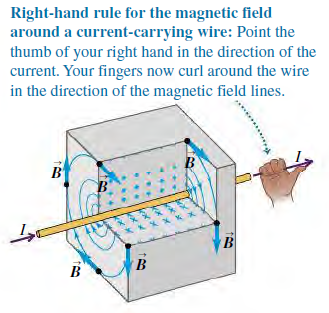
\includegraphics[width=\columnwidth]{Elektro/Figurer/right_hand_rule.PNG}
        \caption{Illustration af højrehåndsreglen for en lige leder. Kilde: figur 28.6 i \cite{youngSearsZemanskyUniversity2016}.}
        \label{fig:right_hand_rule_el}
    \end{subfigure}
    %
    \hfill
    %
    \begin{subfigure}[t]{.47\textwidth}
        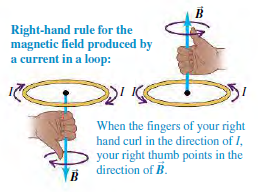
\includegraphics[width=\columnwidth]{Elektro/Figurer/right_hand_rule_loop.PNG}
        \caption{Illustration af højrehåndsreglen for en cirkulær leder. Kilde: figur 28.13 i \cite{youngSearsZemanskyUniversity2016}.}
        \label{fig:right_hand_rule_el_loop}
    \end{subfigure}
    \caption{Illustration af de to versioner af højrehåndsreglen til at finde retningen på et magnetfelt fra en leder.}
    \label{fig:right_hand_rule_both}
\end{figure}

\subsubsection{Højrehåndsreglen}
Det er vigtigt at bemærke at ligning \eqref{eq:b-felt_fra_punktladning} medfører at retningen er givet fra et krydsprodukt af ladningernes bevægelsesretning og en vektor fra ladningen. Højrehåndsreglen for krydsprodukter kan derfor bruges til at finde retninger på magnetfelter. Der er dog en anden højrehåndsregel, der giver samme resultater, som den fra afsnit \ref{fig:right_hand_rule_mat}, som er en fordel at bruge i dette tilfælde. Den fungerer ved at placere højre tommelfinger i strømmens retning eller ladningens bevægelses retning, hvorefter man krøller de andre fingre sammen. Magnetfeltet er så cirkulært om lederen i den retning fingrene peger, se figur \ref{fig:right_hand_rule_el}. Reglen kan også fungere den anden vej rundt, i tilfælde af cirkulær strøm, se figur \ref{fig:right_hand_rule_el_loop}.

\subsection{Amperes lov}
Begrænser man sig til jævne strømme,
%
\begin{align}
    \pdv{\va J}{t} = \pdv{\va I}{t} = 0,
\end{align}
%
viser det sig empirisk at Amperes lov gør sig gældende. Den siger at
%
\begin{align} \label{eq:ampere}
    \oint_P \va B \cdot \dd{\va{l}} = \mu_0 I_\mathrm{inde}.
\end{align}
%
Her angiver $\dd l$ at der er tale om det, der hedder et linjeintegral, hvilket betyder at man integrerer langs en fastlagt linje, og $I_\mathrm{inde}$ er den indesluttede strømstyrke. Den indesluttede strømstyrke er den strømstyrke, der løber igennem den løkke, som den linje man integrerer over. Bemærkelsesværdigt må man vælge en hvilken som helst linje at integrere over, så længe den er lukket, og derefter skal man bruge den tilsvarende strømstyrke. Den linje man integrere over kaldes en Ampereløkke. At Amperes lov er bevist empirisk betyder at de forudsigelser man kan lave med den stemmer overens med eksperimenter, og den kan derfor ikke som sådan udledes matematisk fra noget andet. Det er en abstrakt måde at skrive Amperes lov op, og det tjener det formål at den gælder i alle sammenhænge og i alle koordinatsystemer. For at få en forståelse af hvad det betyder, og hvordan man i praksis bruger ligning \eqref{eq:ampere}, så betragtes et eksempel.
%
\begin{figure}
    \begin{subfigure}{.47\columnwidth}
        \centering
        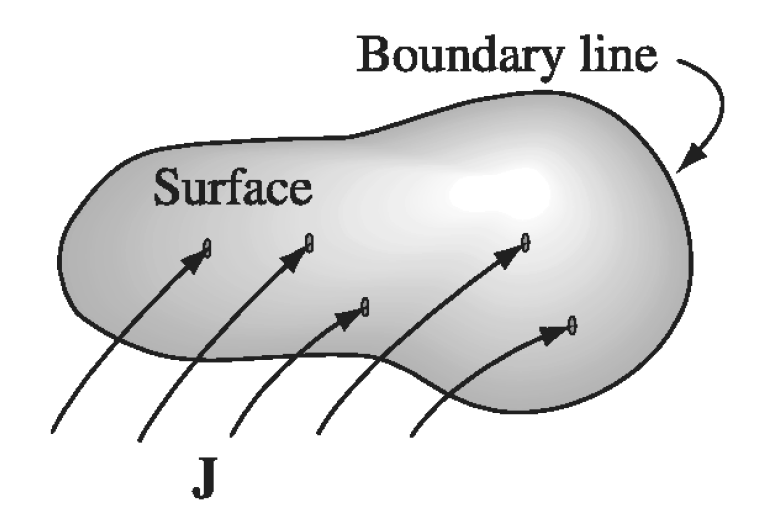
\includegraphics[width=\columnwidth]{Elektro/Figurer/ampere.PNG}
        \caption{Et arbitrært område, hvori der løber en strøm og dermed også en strømtæthed, som så er indrammet af en linje. Kilde: figur~5.31 i \cite{griffithsIntroductionElectrodynamics2017}.}
        \label{fig:ampere}
    \end{subfigure}
%
\hfill
%
    \begin{subfigure}{.47\columnwidth}
        \centering
        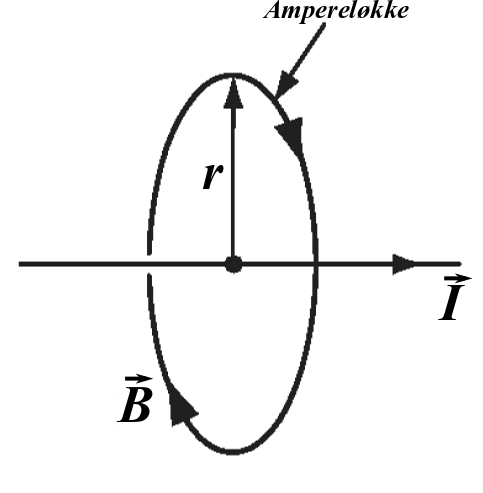
\includegraphics[width=.7\columnwidth]{Elektro/Figurer/lang_lige_leder.PNG}
        \caption{En strømstyrke $I$ løber igennem en uendelig lang lige leder og der placeres en ampereløkke. Kilde: figur~5.32 i \cite{griffithsIntroductionElectrodynamics2017}.}
        \label{fig:lang_lige_leder}
    \end{subfigure}
    \caption{ }
\end{figure}
%
\subsubsection{Den lange lige leder} \label{sec:lang_lige_leder}
Den lange lige leder er et klassisk eksempel på Amperes lov, hvor man bestemmer det magnetiske felt fra en uendelig lang og tynd lige leder overalt i rummet. I første omgang skal man vælge en ampereløkke, hvor der vigtige er at få den valgt så man gør integralet så let for sig selv som muligt. Af højrehåndsreglen fremgår det at magnetfeltet er cirkulært omkring ledningen, hvilket følger af antagelsen om at ledningen er uendelig lang. Hvis lederen ikke havde været uendelig lang ville feltet bøje af i nærheden af kanterne, man da noget uendeligt ikke har nogen kant, så kan feltet kun afhænge af afstanden til ledere - andet ville bryde cylindersymmetrien. Cirklen er smart som ampereløkke, da magnetfeltet så er parallelt med ampereløkken, hvorfor
%
\begin{align}
    \va B \cdot \dd{\va{l}} = B\dd{l},
\end{align}
%
altså blot en skalar og ikke en vektor. Af cylindersymmetrien er størrelsen af magnetfeltet uafhængigt af hvor på løkken man er, hvorfor $B$ er en konstant overfor integrationen:
%
\begin{align}
    \oint_P \va B \cdot \dd{\va{l}} = B \oint_P \dd{l}
\end{align}
%
Prikproduktet skal regnes inden feltet kan trækkes udenfor integralet, da integralet ellers ikke er veldefineret. Et lukket integral over en løkke er løkkens længde, hvilket i det her tilfælde er omkredsen af en cirkel. Yderligere er den indesluttede strøm $I_\mathrm{inde} = I$, hvorfor
%
\begin{align} \label{eq:lang_lige_leder}
    \mu_0I_\mathrm{inde} = B\oint_P \dd{l} = B \cdot 2\pi r  \Rightarrow  B = \frac{\mu_0I}{2\pi r}.
\end{align}
%
Det vigtige når man bruger Amperes lov er symmetri ligesom med Gauss' lov, \eqref{eq:GaussLawGeneral}, og det handler om fysisk at kunne argumentere for magnetfeltets retning overalt i rummet men også hvilke parametre styrken afhænger af og hvor denne er konstant.

\section{Induktion}
Magnetisk induktion er en proces, hvor en ændring i et magnetfelt skaber et elektrisk felt. Mere præcist skaber en ændring i et magnetfelt igennem en løkke et elektrisk felt i selve løkken, som får en strøm til at løbe. For at forstå det skal konceptet om magnetisk flux dog introduceres.

\subsection{Magnetisk flux}
I afsnit \ref{sec:elektrisk_flux} blev konceptet elektrisk flux introduceret som et overfladeintegral. Helt analog defineres den magnetiske flux som
%
\begin{align} \label{eq:magnetisk_flux}
    \Phi_B = \int_S \va B \cdot \dd \va a.
\end{align}
%
Det ses her at magnetisk flux minder meget om integralet i Amperes lov, \eqref{eq:ampere}, men med en meget vigtig forskel - fluxen er et overfalde integral, hvorfor det er et todimensionelt integral defineret ud fra overfladens normalvektor.

\subsection{Faradays lov}
Induktionen er matematisk beskrevet af Faradays lov, der siger at
%
\begin{align} \label{eq:faraday}
    \dv{\Phi_B}{t} = \dv{}{t} \int_S \va B \cdot \dd \va A = - \oint_P \va E\cdot \dd \va l = -\mathcal{E}.
\end{align}
%
$\mathcal{E}$ kaldes den \emph{elektromotoriske kraft} og er en spændingsforskel, som i kredsløbsanalyse ofte betegnes med $V$. %Igennem Ohms lov skaber spændingen en strømstyrke ud fra modstanden i kredsløbet $R$:
%
% \begin{align}
%     I = \frac{U}{R}.
% \end{align}
%
Når man regner induktion, er det også vigtigt, hvilken retning strømmen løber. Dette afgøres med endnu en højrehåndregel, hvor højre tommelfinger placeres i den retning magnetfeltets ændrer sig, hvorefter strømmen løber i den vej rundt i løkken resten af ens fingre peger. Denne højrehåndsregel kaldes Lenz' lov. Det er vigtigt at tommelfingeren placeres i den retning feltet ændrer sig, hvilket kan illustreres med et eksempel. Antag at magnetfeltet igennem en ring er vinkelret på ringens plan, hvilket kaldes $z$-retningen. Skrues der nu op for feltet, ændres det i positiv $z$-retning, hvorfor den inducerede strøm i ringen løber mod uret. I tilfældet hvor feltstyrken mindskes, skal ens tommenfinger pege i negativ $z$-retning, hvorfor den inducerede strøm løber med uret. Figur \ref{fig:right_hand_rule_both} kan derfor bruges, men med den krølle at man i begge figurer skal erstatte $B$ med $\dd{B}/\dd{t}$. \\
%
Det viser sig faktisk at ændringer i elektriske felter også inducerer magnetiske felter. Det hele kommer af at magnetiske felter er introduceret til at håndtere situationer med ladninger i bevægelse. Da felterne opfører sig ret forskelligt, troede man i lang tid også at elektricitet og magnetisme var to forskellige ting, men det viser sig at være to sider af samme sag. Speciel relativitetsteori, der introduceres i kapitel \ref{sec:rela}, beskæftiger sig med hvad der sker, når observatører bevæger sig i forhold til et eksperiment, og det viser sig at et magnetisk felt for en observatør i hvile, er det samme som et elektrisk felt for en observatør i bevægelse sammen med eksperimentet. Det er dog en historie for en anden gang.

\section{Lorentzkraften}
Når nu både elektrostatik (ladninger i hvile) og magnetostatik (ladninger i jævn bevægelse) er introduceret kan den elektriske og magnetiske kraft, ligningerne \eqref{eq:kraft_fra_e-felt} og \eqref{eq:magnetisk_kraft} samles til en elektromagnetisk kraft kaldet Lorenztkraften. Dette gøres med en sum ud fra superpositionsprincippet, der her siger at den totale kraft på et legeme er summen af hvert kraftbidrag. For en partikel med ladning $q$ og hastigheden $\va v$, der bevæger sig i et elektrisk felt $\va E$ og magnetisk felt $\va B$ er Lorentzkraften
%
\begin{align}
    F = q \Big(\va E + \va v \times \va B\Big).
\end{align}
%
Denne formel er relativt simpel og derfor handler store dele af elektromagnetisme om at beregne felterne - man har så at sige gemt det besværlige væk i nogle pæne symboler.

% \newpage
% \section{Opgaver}
\subsection*{Elektrostatik}
\begin{opgave}{Coulombkraften}
    To ladninger, $q_1$ og $q_2$ har en indbyrdes afstand $r$ til hinanden.
    \opg Bestem Coulombkraften fra den ene ladning på den anden i hvert af følgende tilfælde:
    \begin{enumerate}
        \item $r = \SI{1,00}{\metre}$, $q_1 = \SI{1,00}{\coulomb}$ og $q_2 = \SI{1,00}{\coulomb}$
        \item $r = \SI{1,00}{\metre}$, $q_1 = \SI{1,00}{\coulomb}$ og $q_2 = \SI{-1,00}{\coulomb}$
        \item $r = \SI{1,00}{\metre}$, $q_1 = \SI{1,00}{\coulomb}$ og $q_2 = \SI{2,00}{\coulomb}$
        \item $r = \SI{2,00}{\metre}$, $q_1 = \SI{1,00}{\coulomb}$ og $q_2 = \SI{1,00}{\coulomb}$
    \end{enumerate}
    \opg Beskriv med ord hvad der sker med Coulombkraften når den ene ladning skifter fortegn, dens størrelse fordobles og når ladningernes indbyrdes afstand fordobles.
    \opg Brug Newtons anden lov, ligning \eqref{mat:eq:N2}, til at bestemme accelerationen af hver ladning i tilfælde 1. Ladningernes masse er $m_1 = \SI{1,00}{\kilo\gram}$ og $m_2 = \SI{2,00}{\kilo\gram}$.
    \opg Bestem accelerationen af ladning 1 i tilfælde 2-4.
    \opg Beskriv med ord hvad der sker når ladningerne frigives i de fire tilfælde og sammenlign dem.
\end{opgave}

\begin{opgave}{Elektriske feltlinjer}
    Tegn de elektriske feltlinjer for følgende systemer:
    \opg To ladninger $+Q$ og $-2Q$.
    \opg To ladninger $+Q$ og $+2Q$.
    \opg Tre ladninger, $+Q$, som befinder sig på hjørnerne af en ligesidet trekant.
\end{opgave}

% \begin{opgave}{}
%     Skalare størrelser i fysik er bestemt kun med en talværdi, hvorimod vektorer har både en længde og en retning. Men typisk når vi taler om elektrisk strømstyrke har den også en retning. Hvordan tror du man vil kunne definere strømstyrke ud fra en vektor?
% \end{opgave}

\begin{opgave}{Tre ladninger på en linje}
    To punktladninger med ladning $+Q$ befinder sig ved positioner $x=-a$ og $x=a$.
    \opg Bestem kraften på en anden ladning $+q$ som funktion af dens position langs $x$-aksen.
    \opg Tegn en graf over kraften som funktion af position, og kommenter den generelle opførsel.
    \opg Hvordan vil ladningen bevæge sig når den er ved $x=0$?
    \opg For $x\gg a$, approksimer udtrykket for kraften. \textit{Hint: Hvad sker der hvis man lægger et lille tal til et stort tal?}
\end{opgave}

\begin{opgave}{Bohrs atommodel}
    Bohrs atommodel af hydrogenatomet består af en enkelt elektron, som kredser rund om en enkelt proton, i perfekte cirkulære baner. For at opretholde sådan en bane, skal der ifølge Newtons love være en indadgående centripetalkraft $F=mv^2/r$. Antag at elektronen befinder sig i en radius $r=\SI{0.53e-10}{\meter}$ (også kaldet en Bohr radius, $a_0$).
    \opg Hvad er størrelsen af Coulombkraften på elektronen? Dette kan gøres på en af to måder:
    \opg Med Newtonsk mekanik kan det vises at jævn cirkelbevægelse er opfyldt, hvis summen af alle kræfter er ovenstående centripetal kraft. Brug dette til at bestemme elektronens fart i cirkelbanen. \\[4mm]
    Jævn cirkelbevægelse betyder blandt andet at elektronen bevæger sig med samme fart hele tiden. Man kan bruge det til at argumentere for at elektronen kan beskrives med stedfunktionen
    \begin{align*}
        x(t) = vt + x_0,
    \end{align*}
    hvor $v$ er elektronens hastighed, $t$ er tiden og $x_0$ er stedet til tiden $t=0$. \\[4mm]
    Elektronens bane går igennem et område med areal $A$. Argumenter for at den mængde ladningen, der passerer igennem arealet er $q = -neAx(t)$, hvor $n$ er antalstætheden af ladning.
    \opg Estimer ud fra ovenstående strømstyrke en elektron ville generere i hydrogenatomet.
\end{opgave}

\begin{opgave}{Uendelig lang ladet linje}
    For at beregne det elektriske felt overalt i rummet fra en uendelig lang ladet linje med konstant ladningstæthed (ladning pr. afstand) $\lambda$ (med SI-enhed \si{\coulomb\per\meter}) bruges Gauss' lov. Det antages at linjen er i vakuum. En linje har cylindrisk symmetri, hvilket betyder at man kan dreje sit koordinatsystem omkring linjen uden at noget vil ændre sig. Det er derfor smart at bruge en cylinder med længden $L$ og radius $r$ som Gaussisk overflade.
    \opg Tegn situationen.
    \opg Vis at den mængde ladning, som er inden i cylinderen, der bruges som Gaussisk overflade er
    \begin{align*}
        Q_\mathrm{inde} = \lambda L.
    \end{align*}
    \opg Argumenter for at det elektriske felt peger direkte væk fra linjen overalt i rummet.
    \opg Cylinderen har to typer overflade: den krumme og endestykkerne. Udregn $\va E \cdot \dd{\va A}$ i begge tilfælde.
    \opg Det lukkede integral i Gauss' lov kan skrives som en sum af bidragene fra hver overflade. Lad $S_1$ angive den krumme overflade, og henholdsvis $S_2$ og $S_3$ angive de to endestykker. Løs integralet
    \begin{align*}
        \oint_S \va E \cdot \dd{\va A} = \int_{S_1} \va E \cdot \dd{\va A} + \int_{S_2} \va E \cdot \dd{\va A} + \int_{S_3} \va E \cdot \dd{\va A}.
    \end{align*}
    \opg Brug nu Gauss lov til at bestemme det elektriske felt overalt i rummet. \\
    \textit{Hint: Længden af cylinderen skulle gerne gå ud, så det endelige udtryk kun afhænger af $\lambda$, $r$ og nogle konstanter.}
\end{opgave}

\begin{opgave}{Uendeligt ladet plan}
    For at beregne det elektriske felt overalt i rummet fra en uendelig, homogen plan med konstant ladningstæthed (ladning per areal) $\sigma$ (med SI-enhed \si{\coulomb\per\meter\squared}) bruges Gauss' lov. Det antages at planen er i vakuum. Systemet er symmetrisk sådan at man kan spejle sit koordinatsystem i planen uden at noget vil ændre sig. Det er derfor smart at bruge en kvadratisk kasse med sidelængden $L$, hvor overfladen på hver side af planen er afstanden $r$ fra planen, som Gaussisk overflade.
    \opg Tegn situationen.
    \opg Vis at den mængde ladning, som er inden i kasse, der bruges som Gaussisk overflade, er
    \begin{align*}
        Q_\mathrm{inde} = \sigma L^2.
    \end{align*}
    \opg Argumenter for at det elektriske felt peger direkte væk fra planen overalt i rummet.
    \opg Kassen har to typer af overflade: dem som er parallelle med planen og dem, der er vinkelrette på den. Udregn $\va E \cdot \dd{\va A}$ i begge tilfælde.
    \opg Det lukkede integral i Gauss' lov kan skrives som en sum af bidragene fra hver overflade. Lad $S_i$ angive den $i$'te overflade. Løs integralet
    \begin{align*}
        \oint_S \va E \cdot \dd{\va A} = \sum_{i=1}^6 \int_{S_i} \va E \cdot \dd{\va A}.
    \end{align*}
    \opg Brug nu Gauss lov til at vise at det elektriske felt overalt i rummet er
    \begin{align*}
        \va E = \frac{\sigma}{2\epsilon_0}\vu n,
    \end{align*}
    hvor $\vu n$ er en normalvektor til planen.
    \opg Hvordan afhænger størrelsen af E-feltet af hvor i rummet man er?
\end{opgave}

\begin{opgave}{Ladet kugle I}
    En kugle med centrum i origo, $(0,0)$, placeres i vakuum og har den sfærisk symmetriske ladningstæthedsfordelingen
    %
    \begin{align*}
        \rho(r) = \begin{cases} \rho_0(R - r), \quad &r<R \\
        0, \qquad &r>R
        \end{cases} ,
    \end{align*}
    hvor $\rho_0$ og $R$ konstanter. Sfærisk symmetri betyder at $\rho$ kun afhænger af afstanden fra origo. Det er derfor smart at bruge en kugleskal med centrum i $(0,0,0)$, radius $r$ og tykkelse $\dd{r}$ som Gaussisk overfalde.
    \opg Hvad er radius af den ladede kugle?
    \opg Tegn kuglen og den Gaussiske overflade. \\[5mm]
    Nu vil vi gerne bestemme det elektriske felt indeni kuglen
    \opg For en kugleskal kan det vises at $\dd{V} = 4\pi r^2 \dd{r}$. Brug ligning \eqref{eq:volumenladning} til at vise den mængde ladning, som er indenfor kugleskallen, der bruges som Gaussisk overflade, er
    \begin{align*}
        Q_\mathrm{inde} = 4\pi\rho_0\left[\frac{1}{3}Rr^3 - \frac{1}{4}r^4 \right] \quad , \quad r<R.
    \end{align*}
    \opg Argumenter for at det elektriske felt peger direkte væk fra $(0,0)$ overalt i rummet.
    \opg Vis at
    %
    \begin{align*}
        \oint \va E \cdot \dd{\va A} = EA = 4\pi E r^2.
    \end{align*}
    %
    \opg Brug nu Gauss lov til at vise at det elektriske felt inde i kuglen er
    %
    \begin{align*}
        \va E = \frac{\rho_0r}{\epsilon_0}\left(\frac{1}{3}R - \frac{1}{4}r\right)\vu r \quad , \quad r<R,
    \end{align*}
    hvor $\vu r$ er en enhedsvektor, der peger væk fra origo.
    \opg Følg nu fremgangsmåden fra spørgsmål \textbf{2}-\textbf{6} og vis at
    %
    \begin{align*}
        \va E = \frac{\tilde{Q}}{4\pi \epsilon r^2}\vu r \quad , \quad r>R.
    \end{align*}
    %
    $\tilde{Q}$ er en konstant udtrykt ved de tidligere definerede parametre.
    \opg Hvilket kendt system svarer det til?
\end{opgave}

\begin{opgave}{Ladet kugle II}
    En ladet kugle med radius $R$ har en homogen ladningsfordeling $\rho=\rho_0=\text{konstant}$ for $r<R$ og $\rho=0$ for $r>R$, hvor $r$ er afstanden fra kuglens centrum. Kuglen antages at befinde sig i vakuum.
    \opg Hvad betyder det rent fysisk at $\rho(r>R) = 0$?
    \opg Brug Gauss' lov til at bestemme det elektriske felt $\va{E}$ for $r>R$.
    \opg Brug Gauss' lov til at bestemme det elektriske felt $\va{E}$ for $r<R$.
\end{opgave}

\begin{opgave}{Ladet cylinder}
    En uendelig lang cylinder med radius $a$ med ladningsfordelingen
    \begin{align*}
        \rho(r) = \begin{cases}
        \rho_0r/a \: , \quad r<a \\
        0 \: , \qquad r>a
        \end{cases} \: ,
    \end{align*}
    hvor $\rho_0=\text{konstant}$ og $r$ er afstanden fra centrum af cylinderen.
    \opg Brug Gauss' lov til at bestemme det elektriske felt $\va {E}$ i hele rummet.
    \textit{Hint: Se eksemplet i afsnit \ref{sec:gauss_lov_eksempel}.}
\end{opgave}

\begin{opgave}{Cylindrisk ladningsfordeling}
    En arbitrær kontinuert ladningsfordeling med total ladning $+Q$ er placeret i $yz$-planen med centrum i origo, og er rotationssymmetrisk om $x$-aksen. Derudover er en testladning $+q$ placeret et sted langs $x$-aksen. Vi vil gerne bestemme kraften på testladningen som funktion af $x$.
    \opg Betragt to ladninger $+Q/2$, hver især ved en position $y=\pm a$ langs $y$-aksen. Tegn situationen.
    \opg Hvad forventer du at kraften på ladningen $+q$ i de to tilfælde: $x=0$ og $x\gg a$? \textit{Hint: Hvor meget betyder en lille forskel i afstand, når to ting er langt væk fra hinanden?}
    \opg Brug Coulombs lov og superpositionsprincippet til at finde et udtryk for kraften som funktion af $x$.
    \opg Er dette som du forventer? Tegn en graf af $F(x)$ og vis at maksimum er når $x=a/\sqrt{2}$.
    \opg Betragt nu fire ladninger med $+Q/4$. To af dem er placeret på $y$-aksen ved $y=\pm a$, og de to andre på $z$-aksen ved $z=\pm a$. Bestem ligeledes kraften på ladningen $+q$ som funktion af $x$.
    \opg Nu ser vi på et stort antal, $N$, ladninger $+Q/N$, ligeligt fordelt på en cirkel med radius $a$ på $yz$-planet, og med centrum i origo. Hvad er kraften på ladningen $+q$ som funktion af $x$?
    \opg De forrige delopgaver refererer til en \emph{diskret} ladningsfordeling. Betragt nu en \emph{kontinuert} ladningsfordeling: En uendelig tynd ring af radius $a$, med total ladning $+Q$, placeret på $yz$-planet med centrum i origo. Brug dine svar fra de forrige opgaver til at gætte et udtryk for kraften på ladningen $+q$ som funktion af $x$. Brug derefter superpositionsprincippet og integraler til at vise eller afkræfte dit gæt.
    \opg En uendelig tynd, solid disk af radius $a$ og total ladning $+Q$ med ensartet ladningsfordeling er placeret på $yz$-planet med centrum i origo. Vis at kraften på ladningen $+q$ som funktion af $x$ er givet ved
    \[ F(x)=\frac{1}{4\pi\varepsilon_0}\frac{2Qq}{a^2}\left(1-\frac{x}{\sqrt{x^2+a^2}}\right). \]
\end{opgave}

\begin{opgave}{Ladede partikler i en trekant}
    Tre partikel med samme ladning er holdt stille så de danner en (vilkårlig!) trekant. Når der gives slip på partiklerne begynder de at bevæge sig i en lige linje. Vis at hvis dette skal kunne lade sig gøre, så må trekanten de danner til alle tider have samme vinkler som den originale trekant. Du kan antage at de er i vakuum og at ingen andre kræfter påvirker dem.
\end{opgave}

\subsection*{Magnetisme}
\begin{opgave}{Magnetisk felt}
    \opg Bestem det magnetiske felt fra ladningen i punktet $\va r = r \xhat$ i hvert af følgende tilfælde:
    \begin{enumerate}
        \item  $r = \SI{1,00}{\metre}$, $\va{v} = \SI{1,00}{\metre\per\second}\cdot\xhat$ og $q = \SI{1,00}{\coulomb}$
        \item $r = \SI{1,00}{\metre}$,  $\va{v} = \SI{1,00}{\metre\per\second}\cdot\yhat$ og $q = \SI{1,00}{\coulomb}$
        \item $r = \SI{1,00}{\metre}$,  $\va{v} = \SI{1,00}{\metre\per\second}\cdot\zhat$ og $q = \SI{1,00}{\coulomb}$
        \item $r = \SI{1,00}{\metre}$,  $\va{v} = \SI{1,00}{\metre\per\second}\cdot\yhat$ og $q = \SI{-1,00}{\coulomb}$
        \item $r = \SI{1,00}{\metre}$,  $\va{v} = \SI{1,00}{\metre\per\second}\cdot\yhat$ og $q = \SI{2,00}{\coulomb}$
        \item $r = \SI{1,00}{\metre}$,  $\va{v} = \SI{2,00}{\metre\per\second}\cdot\yhat$ og $q = \SI{1,00}{\coulomb}$
        \item $r = \SI{2,00}{\metre}$,  $\va{v} = \SI{1,00}{\metre\per\second}\cdot\yhat$ og $q = \SI{1,00}{\coulomb}$
    \end{enumerate}
    \opg Beskriv med ord hvad der sker med magnetfeltet når ladningen skifter fortegn, dens størrelse fordobles, dens bevægelsesretning ændres, dens hastighed fordobles og når ladningernes indbyrdes afstand fordobles.
    \opg Hvad er den magnetiske kraft på en ladning $Q = \SI{1,00}{\coulomb}$ i punktet $\va r = r \xhat$ med hastigheden $\va v' = \SI{1,00}{\metre\per\second}\cdot\zhat$ i hvert af tilfældende?
\end{opgave}

\begin{opgave}{Uniformt magnetfelt}
    I afsnit \ref{sec:uniformt_b-felt} blev kraften fra et uniformt magnetfelt på en punktladning i bevægelse beregnet.
    \opg Skitser situationen.
    \opg Forklar hvorfor ladningens position ikke blev betragtet i eksemplet.
    \opg Når tiden går ændres retningen på ladningens hastighed. Man kan vise ladningen kommer til at dreje rundt i en cirkel som tiden går. Forklar uden beregninger hvorfor dette sker.
    \opg Hvad ville der ske med ladningen, hvis den havde været påvirket af et uniformt elektrisk felt, $\va E = E_0 \zhat$, og ikke et magnetfelt.
\end{opgave}

\begin{opgave}{Amperes lov}
    Der er to vigtige argumenter i afsnit \ref{sec:lang_lige_leder} og alt kommer fra lederens symmetri og antagelsen om at den er uendelig lang. Forklar med egne ord argumenterne for at
    \opg magnetfeltet er cirkulært omkring lederen.
    \opg magnetfeltets størrelse kun afhænger af afstanden til lederen. \\[4mm]
    Hvis lederen ikke er uendelig lang er ovenstående analyse kun approksimativt sandt omkring midten af lederen.
    \opg Skitser det magnetisk felt for en endelig leder.
\end{opgave}

\begin{opgave}{To lange lige ledere}
    To uendeligt lange lige ledere med strømstyrkerne hhv. $\va I_1 = I_1 \xhat$ og $\va I_2 = I_2 \xhat$ placeres en afstand $d$ fra hinanden.
    \opg Skitser situationen.
    \opg Indtegn et koordinatsystem, hvor $x$-aksen placeres langs med den ene leder.
    \opg Bestem magnetfeltet fra den første leder på den anden.
    \opg Tiltrækkes de to ledere af hinanden eller frastøder de hinanden?
    \opg Hvad hvis strømmen går i hver sin retning af de to ledere?
    \opg Benyt superpositionsprincippet til at beregne magnetfeltet fra de to ledere i tilfældet hvor strømmene er parallelle i $xy$-planen.
\end{opgave}

\begin{opgave}{Forskellen på elektriske og magnetiske felter}
    En ladet partikel bevæger sig i et homogent felt.
    \opg Vis at partiklen altid bevæger sig i en parabel, hvis feltet er elektrisk.
    \opg Sammenlign ovenstående resultat med afsnit \ref{sec:uniformt_b-felt}.
    \opg Hvad ville der ske, hvis ladningen bevægede sig parallelt med et sådant magnetfelt?
\end{opgave}

% \begin{opgave}{}
%     Betragt en ring med total ladning $Q$, vis centrum ligger på $x$-aksen, og alle punkter på cirklen ligger en afstand $r$ fra origo. Linjen fra origo til ethvert punkt på cirklen danner en vinkel $\theta$ med $x$-aksen.
%     \opg Vis at det elektriske felt i origo er
%     \begin{equation}
%         \va{E}=-\frac{Q\cos\theta}{4\pi\varepsilon_0r^2} \xhat.
%     \end{equation}
%     Et dielektrikum med homogen polarisering $\va{P}=P\hat\va{x}$ indeholder et sfærisk hul med radius $r$, centreret i origo.
%     \opg Vis at overfladepolariseringsladningsdensiteten ved ethvert punkt på overfladen af hullet er $\rho_{sp}=-P\cos\theta$, hvor $\theta$ er vinklen mellem linjer fra origo til punktet, og $x$-aksen. Overvej nu et tyndt bånd på overfladen af hullet, hvor linjen der der forbinder origo til ethvert punkt på båndet danner vinklen $\theta$ med $x$-aksen.
%     \opg Vis at den totale ladning på båndet er
%     \begin{equation}
%         Q_\text{bånd}=-2\pi Pr^2\sin\theta\cos\theta\ \dd\theta.
%     \end{equation}
%     \opg Vis dermed at overfladepolariseringsladningen på overfladen af hullet danner et elektrisk felt i origo givet ved
%     \begin{equation}
%         \Delta\Vec{E}=\frac{P}{2\varepsilon_0}\int_0^\pi\sin\theta\cos^2\theta\ \dd\theta \ \xhat.
%     \end{equation}
%     \opg Anvend
%     \[ \int_0^\pi\sin\theta\cos^2\theta\ \dd\theta =\frac{2}{3} \]
%     til at vise at det elektriske felt i centrum af hullet er
%     \begin{equation}
%         \va{E}_\text{hul}=\Vec{E}_\text{diel}+\frac{\Vec{P}}{3\varepsilon_0},
%     \end{equation}
%     hvor $\Vec{E}_\text{diel}$ er det elektriske felt i dielektrikummet.
%     \opg Beregn forholdet mellem $\Vec{E}_\text{diel}$ og $\frac{\Vec{P}}{3\varepsilon_0}$ i glas ($\varepsilon_r=\SI{4.0}{}$).
% \end{opgave}

\begin{opgave}{Lang lige leder med udstrækning}
    I afsnit \ref{sec:lang_lige_leder} blev det magnetiske felt fra en uendelig tynd lang lige leder med strømstyrke $I$ bestemt. Situationen ændrer sig en smule, hvis lederen har en endelig tykkelse $R$, og strømstyrken uniformt fordelt over tværsnittet.
    \opg Argumenter for at udregningerne ikke ændrer sig i en afstand $r>R$, hvorfor magnetfeltet er det samme.
    \opg Argumenter for at integralet i Amperes lov er det samme indenfor og udenfor lederen:
    %
    \begin{align}
        \oint \va B \cdot \dd \va l = 2\pi B r,
    \end{align}
    %
    hvor $r$ er afstanden lederens centrum.
    \opg Vis at den indesluttede strøm i tilfældet $r<R$ er
    %
    \begin{align}
        I_\mathrm{inde} = I \frac{r^2}{R^2}.
    \end{align}
    %
    \opg Brug dette til at vise at
    %
    \begin{align}
        B = \begin{cases}
            \mu_0I/2\pi r, \quad &r>R \\
            \mu_0Ir/2\pi R^2, \quad &r<R
        \end{cases}
        .
    \end{align}
    %
    \opg Skitser funktionen $B(r)$.
    \opg Argumenter kvalitativt for hvordan funktionen $B(r)$ ville se ud hvis lederen var hul med en indre radius $R_0$ og skitser funktionen.
\end{opgave}

\begin{opgave}{Eleveksperiment}
    I et eksperiment har en elev målt strømstyrken gennem en LED over tid og har empirisk estimeret den til at følge funktionen $I=\left(\SI{0.06}{\ampere\second}\right)/\left(\SI{20}{\second}+t\right)$, hvor $t$ er tiden målt i sekunder (målingen starter ved $t=0$).
    \opg Brug at man i fysik godt betragte $\dd{t}$ som en variabel samt ligning \eqref{eq:current} til at vise at
    \begin{align*}
        \dd{q} = I\dd{t}.
    \end{align*}
    \opg Vis at ladningen, der er løbet gennem Amperemeteret i tidsrummet $t=0$ til $t=T$, er
    \begin{align*}
        q(t=T) - q(t=0) = \int_0^T I(t) \dd{t}.
    \end{align*}
    \opg Strømmen i kredsløbet tændes til tiden $t=0$. Hvad er $q(t=0)$?
    \opg Bestem den totale ladning, der har været gennem amperemeteret efter et minut.
\end{opgave}

\begin{figure}
    \centering
    \begin{subfigure}[t]{.47\textwidth}
        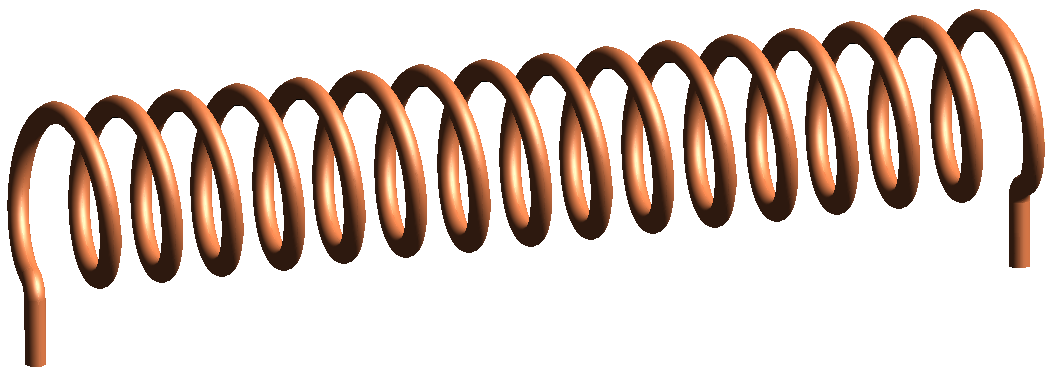
\includegraphics[width=\columnwidth]{opg/figurer/Solenoid-1.png}
        \caption{Illustration af en solenoide. Kilde: \cite{SolenoidWikipedia2019}}
        \label{fig:solenoide}
    \end{subfigure}
    %
    \hfill
    %
    \begin{subfigure}[t]{.47\textwidth}
        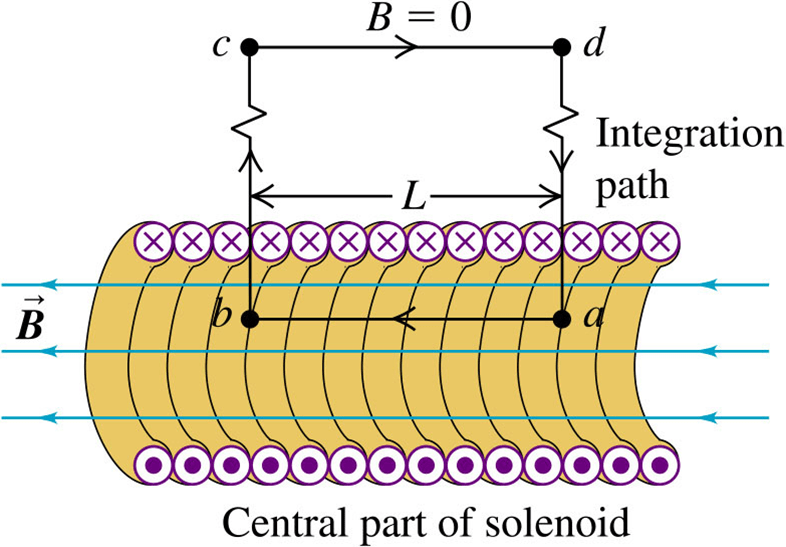
\includegraphics[width=\columnwidth]{opg/figurer/solenoid.png}
        \caption{Tegning af en solenoide med $n$ vindinger pr. længde, hvori der løber en strøm med strømstyrke $I$. Kilde: \cite{UY1ApplicationsAmpere2015}}
        \label{fig:solenoide_ampere}
    \end{subfigure}
    \caption{ }
\end{figure}
\begin{opgave}{Solenoiden}
    Afsnit \ref{sec:uniformt_b-felt} beskrev hvordan en ladning i et uniformt magnetfelt opfører sig. En måde at fremstille et (approksimativt) uniformt magnetfelt er ved brug af en solenoide, som illustreret i figur \ref{fig:solenoide}, hvori en strøm med strømstyrken $I$ løber. Det antages at solenoiden befinder sig i vakuum, at den er meget lang, og at antallet af  vindinger pr. længde, $n$, er så stor at solenoiden kan beskrives som ringe af strøm, der ligger helt tæt op ad hinanden. Der vælges en Ampereløkke, som den i figur \ref{fig:solenoide_ampere}, hvor punkterne $a$ og $b$ placeres midt i solenoiden og punkterne $c$ og $d$ placeres uendeligt langt væk fra solenoiden. Bredden af løkken kaldes $L$ og hele løkken er placeret ved midten af solenoiden.
    \opg Brug højrehåndsreglen til at bestemme retningen på det magnetiske felt midt i solenoiden.
    \opg På baggrund af antagelserne er størrelsen af det magnetiske felt på hele linjestykket $cd$ 0. Forklar hvorfor det er tilfældet.
    \opg Argumenter for at magnetfeltet udenfor solenoiden omkring Ampereløkken er parallelt med feltet indeni solenoiden.
    \opg Brug ovenstående argumenter til at vise at
    \begin{align*}
        \oint_P \va B \cdot \dd{\va l} = BL.
    \end{align*}
    \opg Vis at den indesluttede strøm er
    \begin{align*}
        I_\mathrm{inde} = nLI.
    \end{align*}
    \opg Brug Amperes lov til at vise at magnetfeltet inde i midten af solenoiden er
    \begin{align} \label{eq:b_solenoide}
        B = \mu_0nI.
    \end{align}
    \opg Argumenter, ud fra antagelserne, for at magnetfeltet er uniformt omkring midten af solenoiden med feltstyrken givet i ligning \ref{eq:b_solenoide}.
\end{opgave}

\subsection*{Induktion}
\begin{figure}
    \centering
    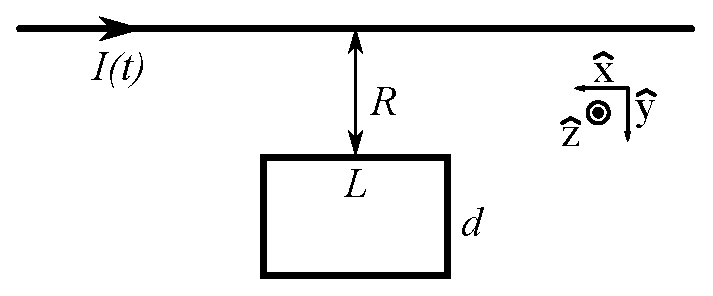
\includegraphics[width=.6\columnwidth]{opg/figurer/induktion.eps}
    \caption{En rektangulær løkke placeret i forhold til en lang lige leder med tidsafhængig strømstyrke.}
    \label{fig:induktion}
\end{figure}
\begin{opgave}{Induktion I}
    En rektangulær løkke af størrelsen $L\times d$ placeres i en afstand $R$ fra en lang lige leder med strømstyrken\footnote{Vekselstrøm kan beskrives med en strømstyrke på denne måde.} $I(t) = I_0\cos(\omega t)$ således at den fjerne del af rektanglen er i afstanden $R+d$ fra fra den lange lige leder -- se figur \ref{fig:induktion}. Induktionen sker i løkken, hvorfor man skal integrere over den overflade løkken udspænder.
    \opg Skraver det område man integrere over i figuren.
    \opg Argumenter for at magnetfeltet i $xy$-planen er uafhængigt af $x$- og $z$-koordinatet, $\va B = \va B(t,y)$.
    \opg Vis at fluxen gennem rektanglen er
    %
    \begin{align}
        \Phi_B = \int_R^{R+d} \int_0^L \va B \cdot \zhat \dd{x}\dd{y} = -\frac{\mu_0LI(t)}{2\pi}\ln\left(\frac{R+d}{R}\right).
    \end{align}
    \opg Vis ved brug af Faradays lov at
    %
    \begin{align}
        \mathcal{E} = \frac{\mu_0LI_0\omega}{2\pi}\ln\left(\frac{R}{R+d}\right)\sin(\omega t).
    \end{align}
    %
    \opg Forklar ud fra Lenz’ lov hvordan strømmen løber i løkken som tiden går.
    \opg En elpære med effekt $P$ tilsluttes løkken. Brug at $P=VI$ til at vise at strømstyrken igennem pæren er
    %
    \begin{align}
        I = \frac{P}{\mathcal{E}} = \frac{2\pi P}{\mu_0LI_0\sin(\omega t)\ln\big[R/(R+d)\big]}.
    \end{align}
\end{opgave}

\begin{figure}
    \centering
    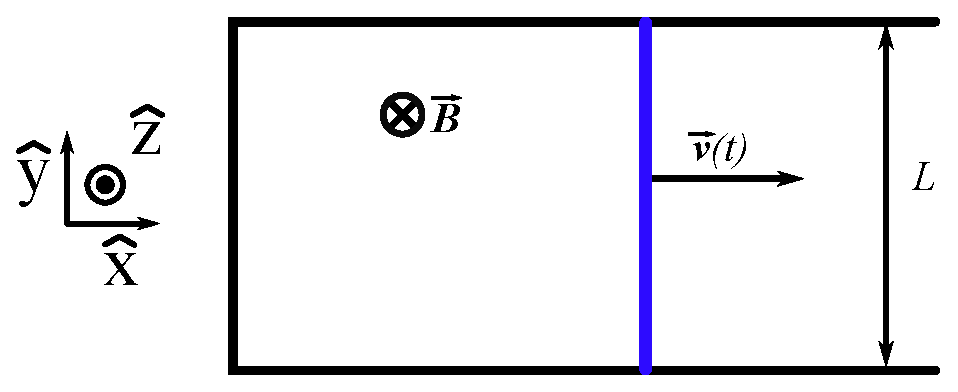
\includegraphics[width=.65\columnwidth]{opg/figurer/induktion_ii.eps}
    \caption{En lineær leder glider vinkelret og friktionsløst med hastighed $v(t)$ på en åben rektangulær leder.}
    \label{fig:induktion_ii}
\end{figure}
\begin{opgave}{Induktion II}
    En lineær leder glider vinkelret og friktionsløst med hastigheden
    %
    \begin{align} \label{eq:fart_induktion}
        \va v(t) = \Big(at + v_0\Big)\xhat
    \end{align}
    %
    på en åben rektangulær leder med bredden $L$, se figur \ref{fig:induktion_ii}. Man kan vise at stedfunktionen for den lineære leder er
    %
    \begin{align} \label{eq:sted_induktion}
        \va r(t) = x(t)\xhat = \left[\frac{1}{2}at^2 + v_0t + x_0\right]\xhat.
    \end{align}
    %
    Opsætningen placeres i et konstant uniformt magnetfelt vinkelret på opstillingen med styrken $\va B(t) = -B_0 \zhat$
    \opg Vis at stedfunktionen \ref{eq:sted_induktion} opfylder at hastighedsfunktionen er ligning \ref{eq:fart_induktion} ud fra definitionen på fart, ligning \ref{mat:eq:hast}.
    \opg Argumenter for at arealelementet i ligning \ref{eq:magnetisk_flux} er
    %
    \begin{align}
        \dd{\va A} = \zhat \dd{x}\dd{y}.
    \end{align}
    %
    \opg Forklar at koordinaterne for hjørnerne i den lukkede rektangel er $(0,0),(0,L),(x(t),L),(x(t),0)$.
    \opg Argumenter for at fluxen er givet ved integralet
    %
    \begin{align}
        \Phi_B = \int_0^L \int_0^{x(t)} \va B \cdot \zhat \dd{x'}\dd{y}.
    \end{align}
    %
    \opg Løs integralet for at vise at
    %
    \begin{align}
        \Phi_B = -B_0L\left[\frac{1}{2}at^2 + v_0t + x_0\right].
    \end{align}
    %
    \opg Vis at den elektromotoriske kraft i kredsløbet er
    %
    \begin{align}
        \mathcal{E} = B_0L\Big[at + v_0\Big].
    \end{align}
    %
    \opg Nu kobles en elpære, der bruger effekten $P$ til kredsløbet. Brug at sammenhængen mellem modstanden, strømstyrke og spændingsforskel er $V^2=PR$ til at vise at modstanden, $R$, i pæren er
    %
    \begin{align} \label{eq:induktion_ii_modstand}
        R(t) = \frac{(B_0L)^2}{P}\Big[at + v_0\Big]^2.
    \end{align}
    %
    \opg Hvilken type funktion er $R(t)$?
    \opg Skitser spændingen som funktion af tid. \\
    \textit{Hint: Det vigtige er hvad der sker over tid, så lad være med at bekymre dig om at tegne funktionen for nogle bestemte værdier af konstanterne.}
    \opg Hvad er modstanden i en $\SI{40}{\watt}$-pære til tiden $t = \SI{0}{\second}$, hvis $B_0 = \SI{1,2}{\tesla}$, $L = \SI{1,5}{\metre}$ og $v_0 = \SI{50}{\kilo\metre\per\hour}$?
\end{opgave}
% \newpage
% \section{Facit}

\setcounter{opgave}{0}

\subsection*{Elektrostatik}

\begin{opgave}{Coulombkraften}
    \opg Indsættes de opgivne tal fås
    \begin{enumerate}
        \item $F = \dfrac{1}{4\pi\epsilon_0}\dfrac{q_1q_2}{r^2} = \SI{8.99e9}{\newton} = \SI{8.99}{\giga\newton}$.
        \item $F = \dfrac{1}{4\pi\epsilon_0}\dfrac{q_1q_2}{r^2} = -\SI{8.99e9}{\newton} = -\SI{8.99}{\giga\newton}$.
        \item $F = \dfrac{1}{4\pi\epsilon_0}\dfrac{q_1q_2}{r^2} = \SI{18.0e9}{\newton} = \SI{18.0}{\giga\newton}$.
        \item $F = \dfrac{1}{4\pi\epsilon_0}\dfrac{q_1q_2}{r^2} = \SI{2.25e9}{\newton} = \SI{2.25}{\giga\newton}$.
    \end{enumerate}
    \[ \]
    \opg Når den ene ladning skifter fortegn, så skifter kraften også fortegn. Fordobles størrelsen af den ene ladning, så fordobles størrelsen af kraften.
    \[ q_1\to -2q_1 \]
    Derudover bliver ladningernes indbyrdes afstand fordoblet.
    \[ r\to 2r\]
    Så vi har at kraften bliver
    \[ F=\frac{1}{4\pi\varepsilon_0}\frac{q_1q_2}{r^2}\to\frac{1}{4\pi\varepsilon_0}\frac{(-2q_1)q_2}{(2r)^2}=-\frac{1}{2}F.\]
    Kraften bliver dermed halvt så stor og skifter retning.
    \opg Vi skal bruge tilfælde 1. fra delopgave 1).
    \[ F=\SI{8.99e9}{\newton} \]
    Her er $m_1=\SI{1.00}{\kilo\gram}$ og $m_2=\SI{2.00}{\kilo\gram}$.
    Accelerationen på de to ladninger er
    \[ a_1 = \dfrac{F}{m_1} = \dfrac{1}{4\pi\epsilon_0}\dfrac{q_1q_2}{m_1r^2} = \SI{8.99e9}{\metre\per\second\squared} \]
    og
    \[ a_2 = \dfrac{F}{m_1} = \dfrac{1}{4\pi\epsilon_0}\dfrac{q_1q_2}{m_2r^2} = \SI{4.49e9}{\metre\per\second\squared}\]
    Her accelererer væk fra hinanden.
    \opg Her fås
    %
    \begin{enumerate}
        \setcounter{enumi}{1}
        \item $a_1 = \dfrac{F}{m_1} = \dfrac{1}{4\pi\epsilon_0}\dfrac{q_1q_2}{m_1r^2} = -\SI{8.99e9}{\metre\per\second\squared} = -\SI{8.99}{\giga\metre\per\second\squared}$.
        \item $a_1 = \dfrac{F}{m_1} = \dfrac{1}{4\pi\epsilon_0}\dfrac{q_1q_2}{m_1r^2} = \SI{18.0e9}{\metre\per\second\squared} = \SI{18.0}{\giga\metre\per\second\squared}$.
        \item $a_1 = \dfrac{F}{m_1} = \dfrac{1}{4\pi\epsilon_0}\dfrac{q_1q_2}{m_1r^2} = \SI{2.25e9}{\metre\per\second\squared} = \SI{2.25}{\giga\metre\per\second\squared}$.
    \end{enumerate}
    I 2. accelererer ladningerne mod hinanden, og væk fra hinanden i 3. og 4.
    \opg Da $m_2 = 2m_1$ accelereres ladning $1$ dobbelt så hurtigt som ladning $2$ uanset hvad kraften er. I tilfælde $1$, $3$ og $4$ har ladningerne samme fortegn, hvorfor de frastøder hinanden og dermed bevæger sig væk fra hinanden. Forskellen på tilfælde $1$ og $3$ er størrelsen på ladningen. Bevægelserne ser derfor ens ud, men alting går dobbelt så hurtigt i tilfælde $3$ som i tilfælde $1$. I tilfælde $4$ starter ladningerne dobbelt så langt fra hinanden som i tilfælde $1$. Selve bevægelsen vil stadig være ens, da det er den samme kraft i begge tilfælde. Alting vil dog gå $1/4$ så langsomt. I disse tre tilfælde vil ladningerne bevæge sig hurtigere og hurtigere væk fra hinanden og forsvinde uendeligt langt væk fra hinanden. Deres acceleration vil dog blive mindre og mindre. I tilfælde $2$ vil de to ladninger tiltrække hinanden, hvorfor de vil bevæge sig tættere og tættere på hinanden. Kraften på dem vil hele tiden øges, hvor accelerationen hele tid stiger. I et kort tidsrum efter de to ladninger frigives vil størrelserne på hastighederne i tilfælde $1$ og $2$ minde om hinanden, men dette holder op med at være tilfældet, når ladningernes indbyrdes afstand har ændret sig betydeligt fra udgangspunktet.
\end{opgave}

\begin{opgave}{Elektriske feltlinjer}
    \opg 
    \begin{figure}[H]
        \centering
        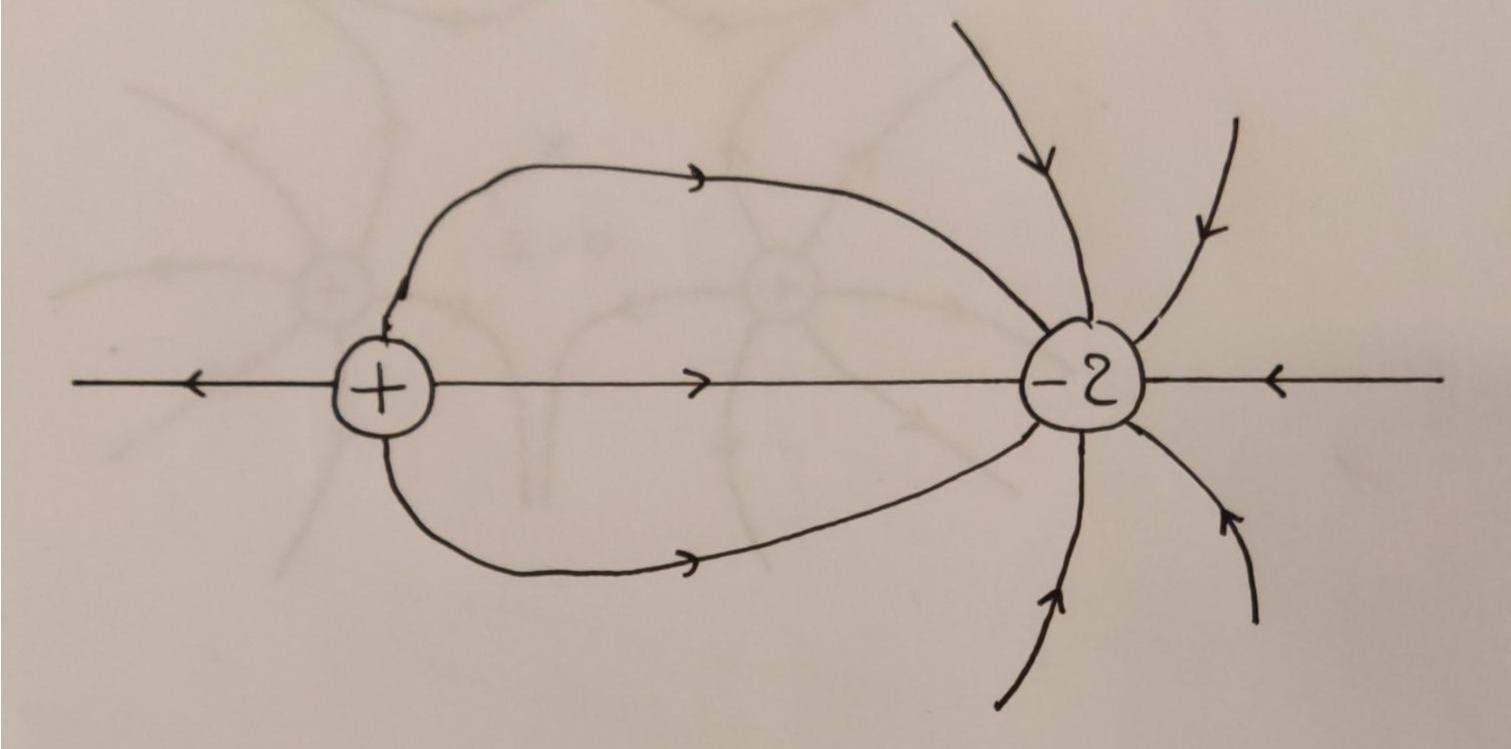
\includegraphics[width=0.8\textwidth]{facit/figurer/elektro/elektro_opg2,1.jpg}
    \end{figure}
    \opg
    \begin{figure}[H]
        \centering
        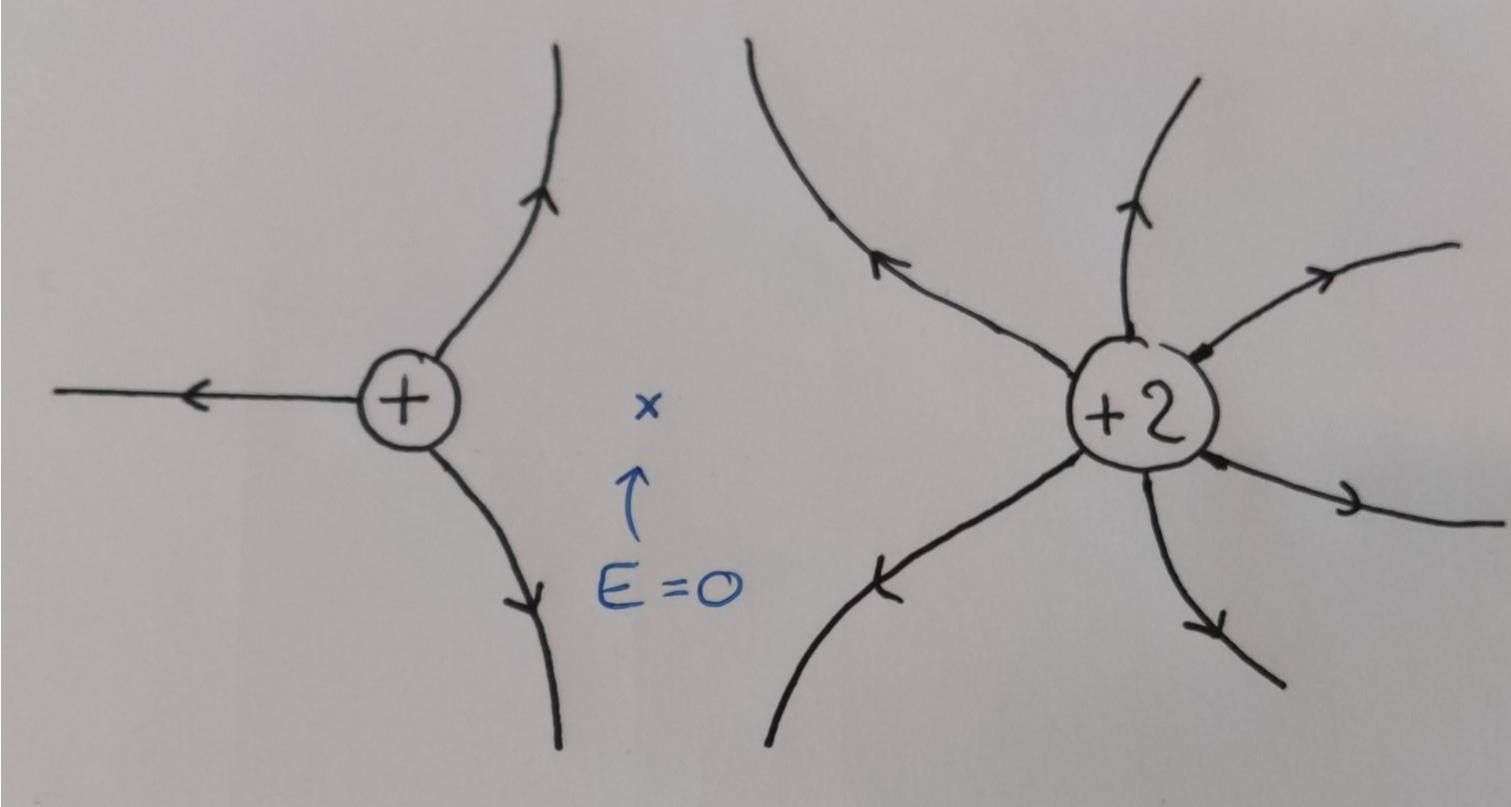
\includegraphics[width=0.8\textwidth]{facit/figurer/elektro/elektro_opg2,2.jpg}
    \end{figure}
    \opg 
    \begin{figure}[H]
        \centering
        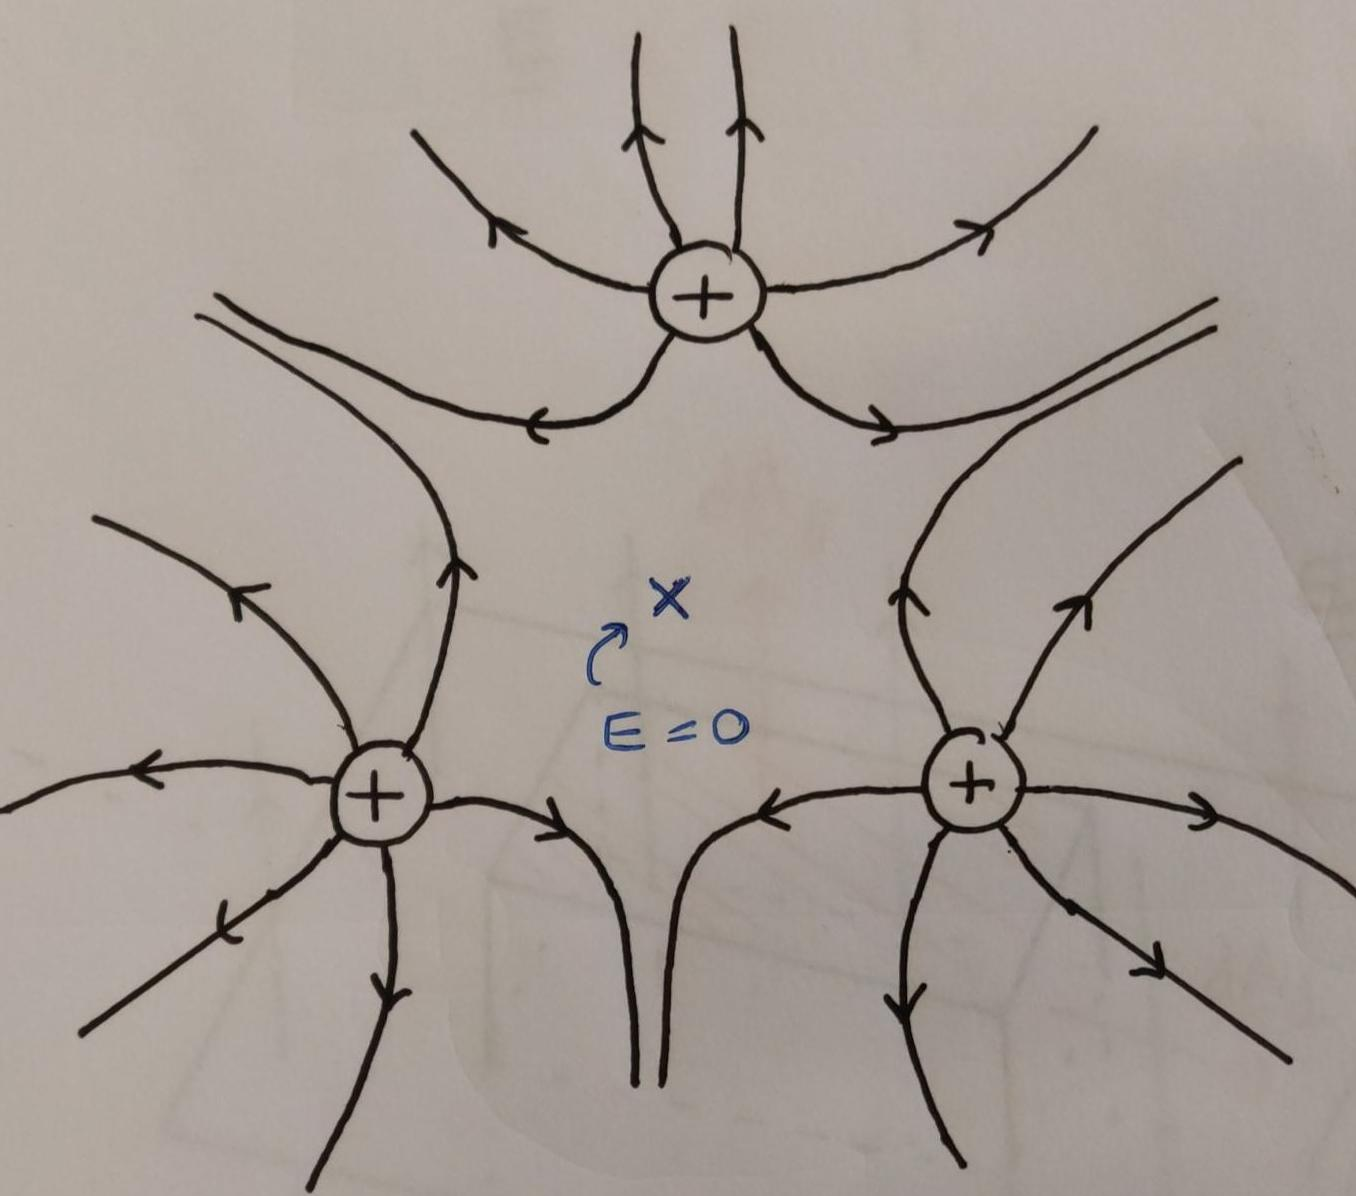
\includegraphics[width=0.8\textwidth]{facit/figurer/elektro/elektro_opg2,3.jpg}
    \end{figure}
\end{opgave}

\begin{opgave}{Tre ladninger på en linje}
    \opg Ved at bruge superpositionsprincippet, bliver dette
    \[ F=\frac{1}{4\pi\varepsilon_0}\left(\frac{Qq}{(x-a)^2}+\frac{Qq}{(x+a)^2}\right). \]
    \opg
    \begin{figure}[H]
        \centering
        \includegraphics[width=0.8\textwidth]{facit/figurer/elektro/elektro_opg3,2.jpg}
    \end{figure}
    \opg Ved $x=0$ så er $F=0$, så ladningen $q$ står stille.
    \opg For $x\gg a$ bliver
    \begin{align*}
        F&=\frac{Qq}{4\pi\varepsilon_0}\left(\frac{1}{(x-a)^2}+\frac{1}{(x+a)^2}\right)\\
        &=\frac{Qq}{4\pi\varepsilon_0}\left(\frac{1}{\left(1-\cancelto{0}{\frac{a}{x}}\right)}+\frac{1}{\left(1+\cancelto{0}{\frac{a}{x}}\right)}\right)\frac{1}{x^2}\\
        &\approx \frac{Qq}{2\pi\varepsilon_0 x^2}\\
        &=\frac{1}{4\pi\varepsilon_0}\frac{(2Q)q}{x^2},
    \end{align*}
    hvilket er kraften på en ladning $q$ pga. en ladning $2Q$ placeret ved $x=0$. Når man er langt væk, kan man nemlig betragte begge $+Q$ ladninger som værende én samlet ladning.
\end{opgave}


\begin{opgave}{Bohrs atommodel}
    \opg Størrelsen af Coulombkraften på elektronen er $|F| = \dfrac{1}{4\pi\epsilon_0}\dfrac{e^2}{r^2} = \SI{8.24e-8}{\newton} = \SI{82.4}{\nano\newton}$.
    \opg Sættes centripetalkraften lig med Coulomkraften fås
    %
    \begin{align*}
        \frac{mv^2}{r} &= \frac{1}{4\pi\epsilon_0}\frac{e^2}{r^2}, \\
        \implies v &= \sqrt{\frac{1}{4\pi\epsilon_0}\frac{e^2}{mr}} = \SI{2.19e6}{\metre\per\second}.
    \end{align*}
    \opg $q(t)$ er en funktion, der beskriver ladningens mængden af ladning inde i området. Tætheden af ladning i bevægelse er $n = \SI{1}{\per\cubic\bohr}$, som bevæger sig i arealet $A = \pi\si{\bohr}^2$. $x(t)$ fortæller placeringen af ladningen og $-\si{\elementarycharge}$ er størrelsen på elektronens ladning. Ganges alle disse størrelser sammen fås en funktion med enheden ladning, der beskriver hvor meget ladning, der er i bevægelse omkring protonen, hvorfor $q(t) = -n\si{\elementarycharge}\pi\si{\bohr\squared}x(t)$ bruges.
    \opg Nu kan ligning \eqref{eq:current} bruges til at estimere strømstyrken en elektron generer i hydrogenatomet.
    %
    \begin{align*}
        I = \dv{q(t)}{t} = -n\si{\elementarycharge}\pi\si{\bohr\squared}\dv{x(t)}{t} = -n\si{\elementarycharge}\pi\si{\bohr\squared}v \approx \SI{20}{\milli\ampere}.
    \end{align*}
\end{opgave}

\begin{opgave}{Uendelig lang ladet linje}
    \opg
    \begin{figure}[H]
        \centering
        \includegraphics[width=0.8\textwidth]{facit/figurer/elektro/elektro_opg5,1.jpg}
    \end{figure}
    \opg Ladningen per længde er $\lambda$. I en $L$ lang cylinder er den samlede ladning derfor
    \[ Q_{inde}=\lambda L. \]
    \opg Reglerne for at tegne feltlinjer siger, at de ikke må røre hinanden. Den eneste retning en feltlinje kan udstrække sig, og fordi der er translatorisk symmetri langs linjen, er derfor væk fra linjen.
    \opg For endestykkerne peger det elektriske felt hen over overfladen, hvilket vil sige at den er vinkelret på arealvektoren. Så $\va E\cdot \dd\va A=0$.\\
    For den krumme overflade peger det elektriske felt vinkelret på overfladen, så $\va E$ og $\dd\va A$ må pege i samme retning. Så $\va E\cdot \dd\va A=E\dd A$.
    \opg Bruger vi ovenstående resultat, bliver integralet
    \begin{align*}
        \oint_S \va E \cdot \dd{\va A} &= \int_{S_1} \cancelto{E\dd A}{\va E \cdot \dd{\va A}} \enspace + \enspace \int_{S_2} \cancelto{0}{\va E \cdot \dd{\va A}} + \int_{S_3} \cancelto{0}{\va E \cdot \dd{\va A}}\\
        &=2\pi r L E
    \end{align*}
    siden $2\pi rL$ er arealet af den krumme overflade på et linjestykke med længde $L$.
    \opg Gauss' lov siger at
    \[ \oint_S \va E\cdot \dd \va A=\frac{Q_\text{inde}}{\varepsilon_0}. \]
    Sætter vi resultatet fra forrige opgave sammen med resultatet for ladningen i lederen, giver det
    \[ 2\pi rLE=\frac{\lambda L}{\varepsilon_0}. \]
    Løses for den elektriske feltstyrke som funktion af afstanden fra lederen, $E(r)$, fås
    \[ E(r)=\frac{\lambda}{2\pi\varepsilon_0 r}. \]
    Hvis vi skal skrive feltstyrken som en vektor, skal vi også kende dens retning. Hvis $\vu r$ er enhedsvektoren der peger væk fra linjen, må
    \[ \va E=E(r)\vu r =\frac{\lambda}{2\pi\varepsilon_0 r}\vu r.\]
    Bemærk, at vektorens størrelse bliver mindre, jo længere væk fra linjen du kommer.
\end{opgave}

\begin{opgave}{Uendeligt ladet plan}
    \opg
    \begin{figure}[H]
        \centering
        \includegraphics[width=0.8\textwidth]{facit/figurer/elektro/elektro_opg6,1.jpg}
    \end{figure}
    \opg Inde i kassen er der en kvadratisk sektion af det ladede plan, med sidelængde $L$. Arealet af planet inde i kassen er derfor $L^2$. Den samlede ladning må være
    \[ Q_\text{inde}=\sigma\cdot\text{Areal}=\sigma L^2. \]
    \opg Per symmetri kan de elektriske feltlinjer ikke pege langs planet, da feltlinjerne ville røre hinanden. Så derfor må de udelukkende pege væk fra planet.
    \opg Fire af kassens sider peger vinkelret på planet. Arealvektoren $\dd \va {A}_\perp$ peger derfor vinkelret med hensyn til de elektriske feltlinjer, så
    \[ \va E\cdot \dd\va {A}_\perp=0. \]
    Toppen og bunden af kassen er overflader der er parallelle med det ladede plan, så $\va E$ må også pege parallelt til arealvektoren, $\dd \va {A}_\parallel$.
    \[ \va E\cdot \dd\va {A}_\parallel = E\dd A_\parallel \]
    Arealet af toppen og bunden af kassen er til sammen $2L^2$, så
    \[ \oint_S \va E\dd \va {A}=2L^2E. \]
    \opg Ved brug af Gauss' lov får man
    \[ \oint_S\va E\dd \va {A}=\frac{Q_\text{inde}}{\varepsilon_0}. \]
    Bruger vi resultaterne fra forrige opgaver giver det ligningen
    \[ 2L^2E=\frac{\sigma L^2}{\varepsilon_0}. \]
    Løses for det elektriske felt, giver det
    \[ E=\frac{\sigma}{2\varepsilon_0}. \]
    Bemærk, at feltstyrken er det samme lige meget, hvor langt væk fra planet man er. Dette er kun sagen, fordi planet udspænder sig uendelig langt.\\
    Der er dog endnu et trin, hvis vi skal skrive feltstyrken som en vektor. Lad os antage, at det uendelige plan ligger i $xy$-planet (med andre ord er $z=0$). Hvis vi ser på positiv $z$, kan vi se at vektoren skal pege opad, mens hvis vi ser på negativ $z$, skal vektoren pege nedad. Derudover ligger $\va E$ altid langs $z$-enhedsvektoren, så
    \[ \va E=\begin{cases*}
    \dfrac{\sigma}{2\varepsilon_0}\vu z & for $z>0$\\
    -\dfrac{\sigma}{2\varepsilon_0}\vu z & for $z<0$
    \end{cases*}.\]
    \opg Som vi så ovenfor, er E-feltets styrke det samme overalt i rummet.
\end{opgave}

\begin{opgave}{Ladet kugle I}
    \opg Radius af den ladede kugle er $R$, da kuglen har ladningsfordelingen $\rho(r) = 0$ for $r > R$.
    \opg 
    \begin{figure}[H]
        \centering
        \includegraphics[width=0.49\textwidth]{facit/figurer/elektro/elektro_opg7,2(1).jpg}
        %
        \includegraphics[width=0.49\textwidth]{facit/figurer/elektro/elektro_opg7,2(2).jpg}
    \end{figure}
    \opg Vi beregner integralet
    \begin{align*}
        Q_\text{inde}&=\int_V\rho\dd V\\
        &=\int_0^r\rho(r)4\pi r^2\dd r\\
        &=\int_0^r 4\pi\rho_0(R_0-r)r^2\dd r\\
        &=4\pi\rho_0\left(\frac{1}{3}R_0r^3-\frac{1}{4}r^4\right)
    \end{align*}
    for $r<R$.
    \opg Per symmetri skal $\va E$ pege væk fra origo.\footnote{Som en analogi, forestil dig hvordan man kan kæmme et pindsvin. Det bliver ikke muligt uden at nogle af piggene peger i en mærkelig retning. Matematisk kaldes dette også for `Hairy Ball Theorem'.}
    \opg Fordi $\va E$ peger vinkelret på overfladen, må den være parallel med arealvektoren. Så
    \[ \va E\cdot \dd\va A=E\dd A. \]
    Overfladearealet af en kugle med radius $r$ er $4\pi r^2$, så
    \[ \va E\cdot \dd\va A=4\pi Er^2. \]
    \opg Gauss' lov er
    \[ \oint \va E\cdot \dd \va A=\frac{Q_\text{inde}}{\varepsilon_0}. \]
    Bruger vi resultaterne fra forrige opgaver får vi
    \[ 4\pi r^2 E=\frac{4\pi\rho_0}{\varepsilon_0}\left(\frac{1}{3}Rr^3-\frac{1}{4}r^4\right) \]
    \[ \Rightarrow E=\frac{\rho_0 r}{\varepsilon_0}\left(\frac{1}{3}R-\frac{1}{4}r\right) \]
    for $r<R$.
    \[ \Rightarrow \va E=\frac{\rho_0 r}{\varepsilon_0}\left(\frac{1}{3}R-\frac{1}{4}r\right)\vu r \]
    \opg Det eneste vi skal beregne igen er ladningen inde i kuglen med radius $r>R$, da ladningsdensiteten er nul udenfor kuglen med radius $R$. Overfladeintegralet giver stadig
    \[ \oint \va E\cdot \dd\va A=4\pi r^2E, \]
    men når vi beregner $Q_\text{inde}/\varepsilon_0$, som er højre side af Gauss' lov, giver det
    \begin{align*}
        \frac{Q_\text{inde}}{\varepsilon_0}&=\frac{1}{\varepsilon_0}\int_0^R 4\pi\rho_0(R-r)r^2\dd r\\
        &=\frac{4\pi\rho_0}{\varepsilon_0}\underbrace{\left(\frac{1}{3}-\frac{1}{4}\right)}_{\text{$1/12$}}R^4\\
        &=\frac{\pi\rho_0}{3\varepsilon_0}R^4
    \end{align*}
    Gauss' lov giver
    \[ 4\pi r^2E=\frac{\pi\rho_0}{3\varepsilon_0}R^4. \]
    Løser vi for $E$, kan vi herefter skrive $\va E=E\vu r$.
    \[ \va E=\frac{1}{4\pi\varepsilon_0}\left(\frac{\pi}{3}\rho_0R^4\right)\frac{1}{r^2}\vu r \]
    Her ser vi at den effektive ladning er
    \[ \widetilde{Q}=\frac{\pi}{3}\rho_0R^4. \]
    \opg Dette svarer til det elektriske felt fra en punktladning $\widetilde{Q}$ placeret i origo.
\end{opgave}

\begin{opgave}{Ladet kugle II}
    \opg Der er ingen ladningsdensitet uden for kuglen. Vi har altså at gøre med en isoleret kugle af ladning.
    \opg Overfladeintegralet på kuglen med radius $r>R$ giver
    \[ \oint\va E\cdot \dd\va A=4\pi r^2E. \]
    Fordi den kugleskal vi ser på er større end selve kugleladningen, må ladningen inden i systemet svare til hele kuglens ladning. Fordi ladningsdensiteten er konstant, ved vi at den samlede ladning er $Q=\rho\cdot\text{Volumen}$, så
    \[ \frac{Q_\text{inde}}{\varepsilon_0}=\frac{4}{3}\pi R^3\rho_0\frac{1}{\varepsilon_0}. \]
    Sætter vi de to lig hinanden giver det
    \[ \va E=\frac{1}{4\pi\varepsilon_0}\underbrace{\left(\frac{4}{3}\pi R^3\rho_0\right)}_{\text{Effektiv ladning, $\tilde{Q}$}}\frac{1}{r^2}\vu r. \]
    \opg Her er ladningen inde i kugleskallen som vi integrerer over, ikke alt ladningen i kuglen. Igen kan vi gange ladningsdensitet med volumen, således at 
    \[ \frac{Q_\text{inde}}{\varepsilon_0}=\frac{4}{3}\pi r^3\rho_0\frac{1}{\varepsilon_0}. \]
    Sætter vi nu
    \[ 4\pi r^2E=\frac{Q_\text{inde}}{\varepsilon_0} \]
    og løser for $E$, giver det til sidst vektoren for den elektriske feltstyrke
    \[ \va E=\frac{\rho_0 r}{3\varepsilon_0}\vu r. \]
\end{opgave}

\begin{opgave}{Ladet cylinder}
    \opg Ligesom for den uendelige lange ladet linje, gælder der per symmetri at $\va E$ peger væk fra centrum af cylinderen.
    \begin{figure}[H]
        \centering
        \includegraphics[width=0.8\textwidth]{facit/figurer/elektro/elektro_opg9,1.jpg}
    \end{figure}
    Betragt en $L$ lang sektion af cylinderen. Overfladeintegralet på cylinderen er
    \[ \oint \va E\cdot \dd\va A=2\pi rLE \]
    som svarer til arealet af den krumme overflade, ganget med feltstyrken, da arealvektoren på enderne af cylinderen står vinkelret på feltlinjerne, så prikproduktet er nul.\\[12pt]
    \underline{$r<a$:} Højre side af Gauss' lov giver
    \begin{align*}
        \frac{Q_\text{inde}}{\varepsilon_0}&=\frac{1}{\varepsilon_0}L\int\rho(r)\dd A\\
        &=\frac{L}{\varepsilon_0}\int_0^r\frac{\rho_0r}{a}2\pi r\dd r\\
        &=\frac{L\rho_0}{\varepsilon_0a}\frac{2\pi}{3}r^3.
    \end{align*}
    Sætter vi de to udtryk lig hinanden får man
    \[ \va E=\frac{\rho_0}{3\varepsilon_0a}r^2\vu r \]
    for $r<a$.\\[12pt]
    \underline{$r>a$:} Udenfor en radius på $a$ er ladningsdensiteten nul, så ladningen inde i den gaussiske cylinder er
    \begin{align*}
        \frac{Q_\text{inde}}{\varepsilon_0}&=\frac{L}{\varepsilon_0}\int_0^a\frac{\rho_0r}{a}2\pi r\dd r\\
        &=\frac{L\rho_0}{\varepsilon_0}\frac{2\pi}{3}a^2.
    \end{align*}
    Sættes dette lig med $2\pi rLE$ og løser man for $E$, giver det
    \[ \va E=\frac{\rho_0 a^2}{3\varepsilon_0 r}\vu r \]
    for $r>a$.
\end{opgave}

\begin{opgave}{Cylindrisk ladningsfordeling}
    \opg
    \begin{figure}[H]
        \centering
        \includegraphics[width=0.8\textwidth]{facit/figurer/elektro/elektro_opg10,1.jpg}
    \end{figure}
    \opg For $x=0$ vil kraften være $F=0$ pga. symmetri.\\
    Ved $x\gg a$ vil $+q$ kun se to ladninger $+Q/2$ placeret meget tæt på hinanden, så essentielt er det en ladning $+Q$ placeret ved $x=0$. Vi forventer derfor at
    \[ F\approx\frac{1}{4\pi\varepsilon_0}\frac{Qq}{x^2}. \]
    \opg Vi ser at per symmetri vil $F_y=F_z=0$ (altså $y$ og $z$ komponenten af $\va F$). Kun $x$ komponenten $F_x$ vil ikke være nul. Ved brug af superpositionsprincippet giver denne
    \begin{align*}
        F_x&=\frac{1}{4\pi\varepsilon_0}\frac{Qq}{2}\underbrace{\left[\frac{1}{x^2+a^2}+\frac{1}{x^2+a^2}\right]}_{\text{$1/r_1^2+1/r_2^2$}}\underbrace{\frac{x}{\sqrt{x^2+a^2}}}_{\text{$\cos(\theta)$}}\\
        &=\frac{Qq}{4\pi\varepsilon_0}\frac{x}{(x^2+a^2)^{3/2}}
    \end{align*}
    \opg Vi vil gerne have, at $F(0)=0$ og
    \[ F(x\gg a)\approx\frac{1}{4\pi\varepsilon_0}\frac{Qq}{x^2}. \]
    Når $x$ er meget lille, vil $x^2\ll a^2$, så det kan vi ignorere i nævneren:
    \begin{align*}
        F_x&\approx \frac{Qq}{4\pi\varepsilon_0}\frac{x}{(a^2)^{3/2}}\\
        &=\frac{Qq}{4\pi\varepsilon_0}\frac{x}{a^3}
    \end{align*}
    Her ses at $F_x\to 0$ når $x\to 0$, som er det vi ønsker.\\
    Når $x$ er meget stor, vil $x^2\gg a^2$, så vi ignorerer i stedet $a^2$ i nævneren:
    \begin{align*}
        F_x&\approx\frac{Qq}{4\pi\varepsilon_0}\frac{x}{(x^2)^{3/2}}\\
        &=\frac{Qq}{4\pi\varepsilon_0}\frac{1}{x^2}
    \end{align*}
    Dette er Coulombs lov, som vi søgte.
    \begin{figure}[H]
        \centering
        \includegraphics[width=0.8\textwidth]{facit/figurer/elektro/elektro_opg10,4.jpg}
    \end{figure}
    For at finde maksimum, differentierer vi $F_x$ med hensyn til $x$ og sætter det lig nul.
    \[ \frac{\dd F_x}{\dd x}=0=\frac{Qq}{4\pi\varepsilon_0}\left[\frac{1}{(x^2+a^2)^{3/2}}-\frac{3}{2}\frac{2x^2}{(x^2+a^2)^{5/2}}\right] \]
    Ved lidt algebraisk gymnastik får man udtrykket
    \[ 3x^2=x^2+a^2. \]
    Dette er en andengradsligning med løsning
    \[ x=\pm \frac{a}{\sqrt{2}}. \]
    \opg Igen er $F_y=F_z=0$ per symmetri. Alle $+Q/4$ ladninger har samme afstand til ladningen $+q$ og $F_x$ komponenten har samme vinkel om $x$-aksen.
    \begin{figure}[H]
        \centering
        \includegraphics[width=0.8\textwidth]{facit/figurer/elektro/elektro_opg10,5.jpg}
    \end{figure}
    Ved brug af superposition får man
    \begin{align*}
        F_x&=\frac{\frac{1}{4}Qq}{4\pi\varepsilon_0}\underbrace{\left[\frac{4}{x^2+a^2}\right]}_{\text{Fire interaktioner}}\frac{x}{\sqrt{x^2+a^2}}\\
        &=\frac{Qq}{4\pi\varepsilon_0}\frac{x}{(x^2+a^2)^{3/2}}
    \end{align*}
    som er det samme udtryk som før.
    \opg Hvis vi følger ovenstående logik, får vi faktisk igen det samme resultat.
    \opg Vi gætter på at vi igen får det samme udtryk, men vi kan også prøve at vise det:
    \begin{figure}[H]
        \centering
        \includegraphics[width=0.8\textwidth]{facit/figurer/elektro/elektro_opg10,7.jpg}
    \end{figure}
    Betragt et infinitesimalt stykke ladning $\delta Q$ langs en cirkel, som tilsammen spænder en vinkel $\delta\phi$. Hvis cirklens totale ladning er $Q$, gælder
    \[ \delta Q=Q\cdot \frac{\delta \phi}{2\pi}. \]
    Kraften forårsaget af det lille stykke ladning må, som vi tidligere har udledt, svare til
    \[ \delta F_x=\frac{\delta Q q}{4\pi\varepsilon_0}\frac{x}{(x^2+a^2)^{3/2}}. \]
    Hvis vi integrerer over hele cirklen, altså en vinkel fra 0 til $2\pi$, må man få hele kraften
    \[ F_x=\int_0^{2\pi}\delta F_x=\frac{Qq}{4\pi\varepsilon_0}\frac{x}{(x^2+a^2)^{3/2}}. \]
    Dette er resultatet som vi gættede.
    \opg Vi kan betragte disken som en masse individuelle ringe af ladning, hver med tykkelse $\delta r$. Ladningen af hver ring er
    \[ Q_\text{ring}=Q\cdot\frac{2\pi r\delta r}{\pi a^2}=\frac{2Qr}{a^2}\delta r, \]
    hvor $Q$ er diskens totale ladning. Så hver ring (med radius $r$) skubber med en kraft
    \begin{align*}
        \delta F_x&=\frac{Q_\text{ring}q}{4\pi\varepsilon_0}\frac{x}{(x^2+r^2)^{3/2}}\\
        &=\frac{Qqrx}{2\pi a^2\varepsilon_0}\frac{1}{(x^2+r^2)^{3/2}}\delta r.
    \end{align*}
    Den samlede kraft pga. alle ringe må derfor være
    \begin{align*}
        F_x&=\frac{Qqx}{2\pi a^2\varepsilon_0}\int_0^a\frac{r}{(x^2+r^2)^{3/2}}\dd r\\
        &=\frac{Qqx}{2\pi a^2\varepsilon_0}\left[-\frac{1}{\sqrt{x^2+r^2}}\right]_0^a\\
        &=\frac{Qq}{2\pi a^2\varepsilon_0}\left(1-\frac{x}{\sqrt{x^2+a^2}}\right).
    \end{align*}
\end{opgave}

\begin{opgave}{Ladede partikler i en trekant}
    \begin{figure}[H]
        \centering
        \includegraphics[width=0.8\textwidth]{facit/figurer/elektro/elektro_opg11.jpg}
    \end{figure}
    Før vi starter med at løse opgaven, giver det god mening af vælge et reference system, når vi ser på vores vektorer. Da alle ladninger flytter sig relativt til hinanden, er det ikke særligt smart at vælge én partikel som origo. Til gengæld viser det sig at være smart, hvis vi vælger massemidtpunktet til at være centrum. Vi noterer at:
    \begin{enumerate}
        \item Der er ingen eksterne krafter på partiklerne, så massemidtpunktet flytter sig aldrig!
        \item Med massemidtpunktet som reference, hvis en partikel bevæger sig i en lige linje, så vil accelerationsvektoren være parallel med positionsvektoren, $\va a\parallel \va r$.
        \item Hvis $\frac{\abs{\va r_i}}{\abs{\va r_j}}$ er konstant for alle $i,j=1,2,3$, så må trekanten være ens hele tiden.\footnote{Med andre ord, hvis forholdene mellem sider på trekanten er konstant, må trekanten til enhver tid være kongruente.}
    \end{enumerate}
    For nemhedens skyld vil vi bruge notationen for Coulombs konstant
    \[ k_c=\frac{1}{4\pi\varepsilon_0}. \]
    Ved brug af superpositionsprincippet og Newtons lov, kan vi skrive kraften på partikel 1 som
    \[ \va F_1=m_1\va a_1=k_c\frac{Q_1Q_2}{d_3^3}(\va r_1-\va r_2)+k_c\frac{Q_1Q_3}{d_2^3}(\va r_1-\va r_3). \]
    Massemidtpunktet kan vi definere på flere forskellige måder:
    \[ \sum_{i=1}^3 m_i\va a_i=\sum_{i=1}^3 m_i\va v_i=\sum_{i=1}^3 m_i \va r_i=0 \]
    Hvis vi substituerer
    \[ \va r_3=-\frac{1}{m_3}\left(m_1\va r_1+ m_2\va r_2\right) \]
    ind i kraftudtrykket får man
    \begin{align*} 
        m_1\va a_1&=k_cQ_1\left(\frac{Q_2}{d_3^3}(\va r_1-\va r_2)+\frac{Q_3}{d_2^3}\left(\va r_1+\frac{m_1}{m_3}\va r_1+\frac{m_2}{m_3}\va r_2\right)\right)\\
        &=k_cQ_1\left[\frac{Q_2}{d_3^3}+\frac{Q_3}{d_2^3}\left(\frac{m_1}{m_3}+1\right)\right]\va r_1 +k_cQ_1\left[\frac{Q_3}{d_2^3}\frac{m_2}{m_3}-\frac{Q_2}{d_3^3}\right]\va r_2.
    \end{align*}
    Hvis partiklerne bevæger sig i en lige linje må det betyde, at $\va a_1$ skal have samme retning som $\va r_1$. I så fald skal komponenten foran $\va r_2$ give 0.
    \[ \frac{Q_3}{d_2^3}\frac{m_2}{m_3}=\frac{Q_2}{d_3^3} \]
    Ved at bytte rundt på variabler i ligningen, og vise samme slags ligninger for de to andre partikler, kan man vise at
    \[ \frac{Q_1d_1^3}{m_1}=\frac{Q_2d_2^3}{m_2}=\frac{Q_3d_3^3}{m_3}. \]
    Med andre ord skal
    \[ \frac{d_1}{d_2}=\sqrt[3]{\frac{Q_2m_1}{Q_1m_2}}=\text{konstant} \]
    \[ \frac{d_2}{d_3}=\sqrt[3]{\frac{Q_3m_2}{Q_2m_3}}=\text{konstant} \]
    \[ \frac{d_3}{d_1}=\sqrt[3]{\frac{Q_1m_3}{Q_3m_1}}=\text{konstant} \]
    Altså har siderne i trekanten konstante forhold. Så trekanten til enhver tid efter vi har sluppet partiklerne må være kongruent til den originale trekant.
\end{opgave}


\subsection*{Magnetisme}

\begin{opgave}{Magnetisk felt}
    \opg Indsættes tallene i formlen fås:
    \begin{enumerate}
        \item $\va B(\va r) = \dfrac{\mu_0}{4\pi}\dfrac{qv\xhat \times r\xhat}{r^3} = \SI{0,00}{\tesla}$.
        \item $\va B(\va r) = \dfrac{\mu_0}{4\pi}\dfrac{qv\xhat \times r\yhat}{r^3} = \SI{1,00e-7}{\tesla}\cdot \zhat$.
        \item $\va B(\va r) = \dfrac{\mu_0}{4\pi}\dfrac{qv\xhat \times r\zhat}{r^3} = -\SI{1,00e-7}{\tesla}\cdot \yhat$.
        \item $\va B(\va r) = \dfrac{\mu_0}{4\pi}\dfrac{qv\xhat \times r\yhat}{r^3} = -\SI{1,00e-7}{\tesla}\cdot \zhat$.
        \item $\va B(\va r) = \dfrac{\mu_0}{4\pi}\dfrac{qv\xhat \times r\yhat}{r^3} = \SI{2,00e-7}{\tesla}\cdot \zhat$.
        \item $\va B(\va r) = \dfrac{\mu_0}{4\pi}\dfrac{qv\xhat \times r\yhat}{r^3} = \SI{2,00e-7}{\tesla}\cdot \zhat$.
        \item $\va B(\va r) = \dfrac{\mu_0}{4\pi}\dfrac{qv\xhat \times r\yhat}{r^3} = \SI{2,50e-8}{\tesla}\cdot \zhat$.
    \end{enumerate}
    \opg Når ladningen skifter fortegn skifter feltet retning. Når ladningen eller farten fordobles gør feltstyrken ligeså. Ændres bevægelsesretning, ændres feltets retning også, således at feltet stadig står vinkelret på stedvektoren og hastighedsvektoren. Fordobles afstanden bliver feltstyrken en fjerdedel af hvad det var før.
    \opg Indsættes tallene i formlen fås:
    \begin{enumerate}
        \item $\va F_{mag} = Q\va v' \times \va B(\va r) = \SI{0,00}{\newton}$.
        \item $\va F_{mag} = Q\va v' \times \va B(\va r) = -\SI{0,00}{\newton}$.
        \item $\va F_{mag} = Q\va v' \times \va B(\va r) = \SI{1,00e-7}{\newton}\cdot \xhat$.
        \item $\va F_{mag} = Q\va v' \times \va B(\va r) = \SI{0,00}{\newton}$.
        \item $\va F_{mag} = Q\va v' \times \va B(\va r) = \SI{0,00}{\newton}$.
        \item $\va F_{mag} = Q\va v' \times \va B(\va r) = \SI{0,00}{\newton}$.
        \item $\va F_{mag} = Q\va v' \times \va B(\va r) = \SI{0,00}{\newton}$.
    \end{enumerate}
    Det bemærkes at opgaven er en smule intetsigende, men ændres hastigheden til $\va{v}' = \SI{1,00}{\metre\per\second}\cdot\xhat$ fås et mere informativt resultat:
    \begin{enumerate}
        \item $\va F_{mag} = Q\va v' \times \va B(\va r) = \SI{0,00}{\newton}$.
        \item $\va F_{mag} = Q\va v' \times \va B(\va r) = -\SI{1,00e-7}{\newton}\cdot\yhat$.
        \item $\va F_{mag} = Q\va v' \times \va B(\va r) = -\SI{1,00e-7}{\newton}\cdot \zhat$.
        \item $\va F_{mag} = Q\va v' \times \va B(\va r) = \SI{1,00e-7}{\newton}\cdot \yhat$.
        \item $\va F_{mag} = Q\va v' \times \va B(\va r) = -\SI{2,00e-7}{\newton}\cdot \yhat$.
        \item $\va F_{mag} = Q\va v' \times \va B(\va r) = -\SI{2,00e-7}{\newton}\cdot \yhat$.
        \item $\va F_{mag} = Q\va v' \times \va B(\va r) = -\SI{2,50e-8}{\newton}\cdot \yhat$.
    \end{enumerate}
\end{opgave}

\begin{figure}
    \centering
    \includegraphics[width=.6\columnwidth]{facit/figurer/elektro/uniformt_felt.eps}
    \caption{Punktladning i uniformt magnetfelt.}
    \label{fig:uniformt_b-felt}
\end{figure}
%
\begin{opgave}{Uniformt magnetfelt}
    \opg Se figur \ref{fig:uniformt_b-felt}.
    \opg Feltet er uniformt, hvilket betyder at det er uafhængigt af sted. Der er derfor ingen grund til at bekymre sig om det.
    \opg Kraften, og dermed accelerationen, står altid vinkelret på feltet og hastigheden. Det samme gør sig gældende, hvis man spænder en sten fast i en snor og derefter får stenen til at dreje rundt. Stenen vil gerne fortsætte i den retning den har, men snoren trække den hele tiden ind mod ens hånd. Denne retning ændrer sig hele tiden, hvorfor bevægelsen kontinuerligt bliver afbøjet ind mod et punkt. Dette betyder at stenen kommer til at bevæge sig langs en cirkel. Det samme sker for ladningen i dette tilfælde. Den bliver hele tiden trukket mod et punkt, men pga. dens hastighed rammer den hele tiden ved siden af og ender med at være fastholdt i en cirkelbevægelse.
    \opg Ladningen ville i så fald blive accelereret med konstant acceleration i $z$-retningen, hvilket giver en parabelbevægelse -- se opgave \thechapter\ref{opg:EvsB}. Dette er det samme som tyngdekraften, hvorfor ladningen vil opføre sig som et skråt kast.
\end{opgave}

%
\begin{figure}
    \centering
    \includegraphics[width=.5\columnwidth]{facit/figurer/lige_leder.eps}
    \caption{Endelig lige leder med dens magnetiske feltlinjer i blå.}
    \label{fig:lige leder}
\end{figure}
%
\begin{opgave}{Amperes lov}
    Der er to vigtige argumenter i \ref{sec:lang_lige_leder} og alt kommer fra lederens symmetri og antagelsen om at den er uendelig lang. Forklar i det eget sprog argumenterne for at
    \opg Lederen er uendeligt lang, strømstyrken er den samme hele vejen igennem og cylindrisk symmetrisk. Det betyder at man ikke kan se forskel på forskellige steder på lederen. Feltet skal have samme symmetri, hvorfor man ikke vil kunne se forskel på feltet forskellige steder i retningen langs med lederen. Det betyder at feltet ikke kan have nogen komposant i retningen langs med lederen -- med andre ord går feltet rundt om lederen i et plan vinkelret på lederen og har form som enten ellipser eller cirkler. Da lederen er cylindrisk symmetrisk, kan man heller ikke se forskel på hvilken retning man kigger væk fra lederen. Står man i midten af en ellipse, ser den ikke ens ud i alle retninger, hvorfor den ikke har den korrekte symmetri. Den eneste mulige form feltlinjerne kan have er derfor cirkler med lederen i centrum.
    \opg Det tredimensionelle rum kan beskrives med tre koordinater. Det kan være de kartetiske $(x,y,z)$, men også de cylindriske koordinater $(r,\phi,z)$, hvor $r$ er afstanden vinkelret fra lederen, $\phi$ er den vinkel, der fortæller i hvilken retning vinkelret fra lederen man kigger, og $z$ er koordinatet langs lederen. Af ovenstående ser situationen ens ud ligegyldigt hvilket $z$-koordinat man vælger -- ergo må feltet være uafhængig at $z$. Ligeledes må de se ens ud ligegyldig hvilket $\phi$ man vælger, hvorfor feltet heller ikke må afhænge af dette koordinat. Feltet er dog ikke ens i hele rummet, da feltstyrker afhænger af hvor langt man er fra lederen, men dette er det eneste koordinat feltstørrelsen afhænger af.
    \opg Se figur \ref{fig:lige leder}.
\end{opgave}

\begin{figure}
    \centering
    \includegraphics[width=.5\columnwidth]{facit/figurer/elektro/to_lange_lige_leder.eps}
    \caption{Skitse af situationen med de to lange lige ledere.}
    \label{fig:to_lange_lige_ledere}
\end{figure}
\begin{opgave}{To lange lige ledere}
    \opg Se figur \ref{fig:to_lange_lige_ledere}.
    \opg Se figur \ref{fig:to_lange_lige_ledere}.
    \opg Magnetfeltet fra en lang lige leder er givet ved ligning \eqref{eq:lang_lige_leder}, og af højrehåndsreglen er magnetfeltet fra den øverste leder på den nederste
    %
    \begin{align*}
        \va B = -\frac{\mu_0I_1}{2\pi d}\zhat.
    \end{align*}
    %
    \opg Da $\va I_2 = I_2\xhat$ så bevæger ladningerne sig i positiv $x$-retning. Det betyder at $\va v \times \va B \parallel \xhat \times (-\zhat) = \yhat$, hvilket er i retning af den anden leder. Ergo tiltrækkes lederne af hinanden. Dette kan også argumenteres med højrehåndsreglen for krydsproduktet.
    \opg I så fald ville der komme et ekstra fortegn i krydsproduktet, hvorved $\va v \times \va B \parallel (-\xhat) \times (-\zhat) = -\yhat$, hvorfor de frastøder hinanden. Igen fås det samme med højrehåndsreglen.
    \opg $x$-aksen placeres parallelt med den øverste leder. Det betyder at denne leder har $y$-koordinat $y_1 = 0$, mens den nederste leder har $y$-koordinat $y_2 = -d$. Da det ikke nødvendigvis er trivielt hvordan fortegnene ordner sig tages det i tre tilfælde. Først kigges på $y>0$: Her er giver begge ledere et bidrag i positiv $z$-retning, hvilket kan ses med højrehåndsreglen, hvorfor superpositionsprincippet giver at
    %
    \begin{align*}
        \va B = \frac{\mu_0}{2\pi}\left(\frac{I_1}{y} + \frac{I_2}{y+d}\right)\zhat \quad , \quad y > 0.
    \end{align*}
    %
    For $y<-d$ fås tilsvarende at
    %
    \begin{align*}
        \va B = \frac{\mu_0}{2\pi}\left(\frac{I_1}{y} + \frac{I_2}{y-d}\right)\zhat \quad , \quad y < -d.
    \end{align*}
    %
    Bemærk at feltet her peger i negativ $z$-retning da både $y$ og $y-d$ er negative tal. I tilfældet $-d<y<0$ giver de to ledere et bidrag i hver sin retning. $I_1$ giver et bidrag i negativ $z$-retning, hvilket det negative $y$-koordinat sørger for. $I_2$ giver et bidrag i positiv $z$-retning. Dette fås med feltet
    %
    \begin{align*}
        \va B = \frac{\mu_0}{2\pi}\left(\frac{I_1}{y} + \frac{I_2}{y+d}\right)\zhat \quad , \quad -d < y < 0.
    \end{align*}
    %
    Som test indsættes $y = -d/2$, hvorved det første led bliver negativt, mens det andet led bliver positivt. Yderligere går det andet led mod uendeligt i grænsen $y \rightarrow -d$, hvorfor den korrekte konstellation er opnået. Samles det fås at magnetfeltet i $xy$-planen er
    %
    \begin{align}
        \va B(y) = \begin{cases}
            \frac{\mu_0}{2\pi}\left(\frac{I_1}{y} + \frac{I_2}{y+d}\right)\zhat, \quad &y>-d \\
            \frac{\mu_0}{2\pi}\left(\frac{I_1}{y} + \frac{I_2}{y+d}\right)\zhat, \quad &y<-d
        \end{cases}
        .
    \end{align}
    %
\end{opgave}

\begin{opgave}{Forskellen på elektriske og magnetiske felter} \label{opg:EvsB}
    \opg Da feltet er homogent, har det samme størrelse og retning overalt i rummet. Lad $\vu e$ betegne en enhedsvektor i det elektriske felts retning, da kan feltet skrives som $\va E = E\vu e$. Af ligning \eqref{eq:e-felt_def} er kraften på en ladning $q$
    %
    \begin{align*}
        \va F = qE\vu e,
    \end{align*}
    %
    hvor længden af vektoren er konstant. Kaldes ladningens masse $m$ kan Newtons 2. lov, ligning \eqref{mat:eq:N2}, bruges til at bestemme accelerationen af ladningen:
    %
    \begin{align*}
        \dv[2]{\va r}{t} = \va a = \frac{qE}{m}\vu e.
    \end{align*}
    %
    Dette er en differentialligning, der kan løses ud fra tabel \ref{mat:tab:diffligninger}, hvorefter man får
    %
    \begin{align*}
        \va r(t) = \frac{1}{2}\frac{qE}{m}t^2\vu e + \va v_0 t + \va r_0,
    \end{align*}
    %
    hvor $\va v_0$ er hastigheden til tiden $t=0$, hvor feltet tændes, og $\va r_0$ er positionen til samme tid. Dette genkendes som en parabel, hvormed det ønskede er vist.
    \opg Først og fremmest bemærkes det at bevægelsen er afhængig af partiklens hastighed i stedet for at være uafhængig af sted og hastighed. Det er derfor sværere at løse differentialligningen generelt, men ikke umuligt. Elektriske felter påvirker ladninger med en kraft i samme retning som feltet. Grundet krydsproduktet i ligning \eqref{eq:magnetisk_kraft} er kraften altid vinkelret på ladningens bevægelsesretning. Dette er karakteristisk for en cirkelbevægelse omkring feltets akse. Er der tale om et homogent magnetisk felt fås derfor en spiralbevægelse omkring feltets akse, og i tilfældet hvor starthastigheden i $z$-retningen er $v_z = 0$ er ladningen i jævn cirkelbevægelsen.
    \opg I dette tilfælde er $\va v \parallel \va B$. Krydsproduktet af to parallelle vektorer er altid nul, $\va v \times \va B = \va 0$, hvorfor ladningen ikke vil blive påvirket af feltet.
\end{opgave}

\begin{opgave}{Lang lige leder med udstrækning}
    I afsnit \ref{sec:lang_lige_leder} blev det magnetiske felt fra en uendelig tynd lang lige leder bestemt. Situationen ændrer sig en smule, hvis lederen har en endelig tykkelse $R$.
    \opg Retningen på feltet ændrer sig ikke af at lederen ikke er uendelig tynd, hvorfor $\oint \va B \cdot \dd \va l$ forbliver uændret. Strømmen $I$ er nu fordelt ud over en leder, men så længe Ampereløkken er udenfor lederen, er der ikke ændret på hvor meget strøm, der er inden i lederen hvorfor $I_\mathrm{inde}$ forbliver uændret. Derved er udregningen og således resultatet helt det samme for $r>R$.
    \opg Af ovenstående sker der intet nyt udenfor lederen. Indenfor lederen er magnetfeltet stadig cirkulært, da magnetfeltet har samme cylindriske symmetri som lederen, hvorfor feltet alle steder er parallelt med integrationslinjen. Integralet bliver derfor cirklens omkreds gange feltstyrken,
    %
    \begin{align}
        \oint \va B \cdot \dd \va l = 2\pi B r.
    \end{align}
    %
    \opg Strømtætheden over cylinderens tværsnit er af ligning \eqref{eq:current_density} $J = I/\pi R^2$. Da strømmen er uniformt fordelt, så er $J$ konstant over hele tværsnittet. Derfor er
    %
    \begin{align}
        I_\mathrm{inde} = JA_\mathrm{inde}= \frac{I}{2\pi R^2} 2\pi r^2 = I \frac{r^2}{R^2}.
    \end{align}
    %
    \opg Bruges Amperes lov fås nu at for $r<R$ er
    %
    \begin{align*}
        \oint \va B \cdot \dd \va l = \mu_0I_\mathrm{inde} \implies 2\pi B r = \mu_0I \frac{r^2}{R^2} \implies B = \frac{\mu_0Ir}{2\pi R^2}.
    \end{align*}
    %
    Af spørgsmål 1 fås således at
    %
    \begin{align*}
        B = \begin{cases}
            \mu_0I/2\pi r, \qquad &r>R \\
            \mu_0Ir/2\pi R^2, \quad &r<R
        \end{cases}
        .
    \end{align*}
    %
    \begin{figure}
        \centering
        \begin{subfigure}[t]{.47\textwidth}
            \centering
            \includegraphics[width=\columnwidth]{facit/figurer/elektro/lange_lige_leder_cylinder.eps}
            \caption{Cylindrisk leder med radius $R$.}
            \label{fig:lang_lige_cylindrisk_leder}
        \end{subfigure}
        %
        \hfill
        %
        \begin{subfigure}[t]{.47\textwidth}
            \centering
            \includegraphics[width=\columnwidth]{facit/figurer/elektro/lange_lige_leder_hul_cylinder.eps}
            \caption{Hul cylindrisk leder med indre radius $a = R/2$ og ydre radius $R$.}
            \label{fig:lang_lige_hul_cylindrisk_leder}
        \end{subfigure}
        \caption{Størrelsen af af magnetfeltet for en lang lige leder med uniform strømfordeling som funktion af afstanden fra lederens centrum. Feltstyrken er angivet i enheder af den maksimale feltstyrke, $B(r/R)$.}
    \end{figure}
    %
    \opg Se figur \ref{fig:lang_lige_cylindrisk_leder}
    \opg Da cylinderen er hul med en indre radius $a$, løber der ingen strøm i området $r<a$. Ampereløkken kan vælges arbitræt indeni hulrummet uden at den vil indeslutte nogen strøm. For at opfylde Amperes lov må magnetfeltet derfor være nul i hulrummet og derfra har den samme form som for cylinderen uden hulrum, se figur \ref{fig:lang_lige_hul_cylindrisk_leder}.
\end{opgave}

\begin{opgave}{Eleveksperiment} \label{opg:EleveksperimentFacit}
    \opg Ligning \ref{eq:current} siger, at $I \equiv \dv{q}{t}$, og da vi må betragte $\dd{t}$ som en variabel, så må vi gange med den, så
    \begin{align} \label{eq:dq=Idt}
        \dd{q} = I \dd{t} \: .
    \end{align}
    \opg Vi kan nu integrere op ligning \ref{eq:dq=Idt}, hvor vi, når vi integrerer mht. $t$, integrerer fra $0$ til $T$ (det givne tidsrum), og integralet mht. $q$ integreres fra $q(t = 0)$ til $q(t = T)$. Vi får derved integralerne
    \begin{align}
        \int_0^T I(t) \, \dd{t} &= \int_{q(t = 0)}^{q(t = T)} \dd{q}
            = \left[q\right]_{q(t = 0)}^{q(t = T)}
            = q(t = T) - q(t = 0) \: .
    \end{align}
    \opg Idet strømmen først tændes til tiden $t = 0$, da vil der til $t=0$ ikke være nogen ladning:
    \begin{align}
        q(t = 0) &= 0 \: .
    \end{align}
    \opg Den totale ladning gennem amperemeteret efter et minut findes ved at indsætte $60$ sekunder (1 min) i stedet for $T$ i ligningen fra opgave \thechapter,\ref{opg:EleveksperimentFacit} delopgave 2, hvor $q(t = 0) &= 0$, så
    \begin{align}
        q(\SI{60}{\second}) &= \int_0^T I(t) \, \dd{t}
            = \int_{\SI{0}{\second}}^{\SI{60}{\second}} \frac{\SI{0,06}{\ampere\second}}{\SI{20}{\second} + t} \, \dd{t}
            = \left[\SI{0,06}{\ampere\second} \cdot \ln\left(\SI{20}{\second} + t\right)\right]_{\SI{0}{\second}}^{\SI{60}{\second}} \nonumber\\
            &= \SI{0,06}{\ampere\second}\left\{\ln\left(\SI{20}{\second} + \SI{60}{\second}\right) - \ln\left(\SI{20}{\second} + \SI{0}{\second}\right)\right\}
            = \SI{0,06}{\ampere\second}\left\{\ln\left(\SI{80}{\second}\right) - \ln\left(\SI{20}{\second}\right)\right\} \nonumber\\
            &= \SI{0,06}{\ampere\second} \cdot \ln\left(\frac{\SI{80}{\second}}{\SI{20}{\second}}\right)
            = \SI{0,06}{\ampere\second} \cdot \ln(4)
            = \SI{0,083}{\coulomb} \: .
    \end{align}
\end{opgave}

\begin{opgave}{Solenoiden}
    \opg Samme vej som indikeret på figur \ref{fig:solenoide_ampere}.
    \opg Linjestykket $cd$ er uendelig langt væk. Elektriske og magnetiske felter går, som tommelfingeregel, som $1/r^2$, hvilket betyder at de bliver mindre og mindre desto længere væk fra kilden man er. Er man uendelig langt væk, må feltet være uendelig småt, hvilket i fysikermatematik er det samme som 0.
    \opg Solenoiden er pr. antagelse meget lang ift. Ampereløkken. Feltlinjerne skal være kontinuerte og har form som en udstrukket ellipse, der indeslutter en del af solenoiden. Grundet solenoidens længde er ellipsen strukket så meget at den omkring midten af solenoiden er parallel med solenoiden -- dette gælder båden indenfor og udenfor solenoiden.
    \opg Af ovenstående er feltet vinkelret på, linjestykkerne $bc$ og $da$, hvorfor $\va B \cdot \dd{\va l} = 0$. For linjestykke $cd$ er feltet 0, hvorfor integralet også er, mens $\va B \cdot \dd{\va l} = B\dd{l}$ Ergo bliver det lukkede linjeintegral
    \begin{align*}
        \oint_P \va B \cdot \dd{l} = \int_{ab} B\dd{l} = B\int_0^L \dd{l} = BL.
    \end{align*}
    %
    \opg Den indesluttede strøm er antallet af ringe, som løkken indeslutter, $nL$, gange strømstyrken af strømmen i en enkelt leder, $I$. Ergo er
    \begin{align*}
        I_\mathrm{inde} = nLI.
    \end{align*}
    \opg Nu sættes informationerne ind i Amperes lov, ligning \eqref{eq:ampere}, hvor der fås
    \begin{align*}
        \oint_P \va B \cdot \dd{\va{l}} = \mu_0 I_\mathrm{inde} \implies BL = \mu_0nLI \implies B = \mu_0nI
    \end{align*}
    \opg Præcis i midten af solenoiden skal feltet være parallelt med solenoiden for at bevare den cylindriske symmetri. Tæt på midten er ellipserne så store, at der ikke er den store afvigelse fra de rette linjer, hvorfor feltet er nogenlunde uniformt
\end{opgave}


\subsection*{Induktion}

\begin{figure}
    \centering
    \includegraphics[width=.6\columnwidth]{facit/figurer/elektro/induktion_svar.eps}
    \caption{Skravering af det område løkken omkranser.}
    \label{fig:induktion_svar}
\end{figure}
%
\begin{opgave}{Induktion I}
    \opg Se figur \ref{fig:induktion_svar}.
    \opg Af argumenterne i afsnit \ref{sec:lang_lige_leder} er magnetfeltet fra en lang lige leder i et punkt kun afhængigt af afstanden fra lederen til punktet. I $xy$-planen er de beskrevet ved $y$-koordinatet, hvorfor magnetfeltet er uafhængigt af $x$- og $z$-koordinatet.
    \opg Fluxen gennem rektanglen er overfladeintegralet af magnetfeltet i det område. Hele rektanglen ligger i $xy$-planen, hvorfor dens arealelement er
    %
    \begin{align*}
        \dd{\va A} = \zhat\dd{x}\dd{y}.
    \end{align*}
    %
    Af højrehåndsreglen peger magnetfeltet ind i løkken og udskiftes $r$ med $y$ i ligning \eqref{eq:lang_lige_leder} er
    %
    \begin{align*}
        \va B = -\frac{\mu_0I(t)}{2\pi y}\zhat.
    \end{align*}
    %
    Koordinatsystemets nulpunkt vælges som vist på figur \ref{fig:induktion_svar}, og da $\zhat\cdot\zhat = 1$ bliver fluxen
    %
    \begin{align*}
        \Phi_B &= \int_R^{R+d} \int_0^L \va B \cdot \zhat \dd{x}\dd{y} = -\int_R^{R+d} \int_0^L \frac{\mu_0I(t)(t)}{2\pi y} \dd{x}\dd{y} = -\frac{\mu_0I(t)}{2\pi} \int_R^{R+d} y^{-1} \int_0^L \dd{x}\dd{y} \\
        &= -\frac{\mu_0I(t)}{2\pi} \int_R^{R+d} y^{-1} \Big[x\Big]_0^L \dd{y} = -\frac{\mu_0I(t)}{2\pi} \int_R^{R+d} y^{-1} L \dd{y} = -\frac{\mu_0LI(t)}{2\pi} \int_R^{R+d} y^{-1} \dd{y} \\
        &= -\frac{\mu_0LI(t)}{2\pi} \Big[\ln(y)\Big]_R^{R+d} = -\frac{\mu_0LI(t)}{2\pi} \Big[\ln(R+d) - \ln(R)\Big] = -\frac{\mu_0LI(t)}{2\pi}\ln\left(\frac{R+d}{R}\right).
    \end{align*}
    %
    \opg Først indsættes udtrykket for $I(t)$ i ovenstående flux og derefter bruges Faradays lov:
    %
    \begin{align*}
        \mathcal{E} &= -\dv{\Phi_B}{t} = \frac{\mu_0L}{2\pi}\ln\left(\frac{R+d}{R}\right)\dv{I(t)}{t} = \frac{\mu_0L}{2\pi}\ln\left(\frac{R+d}{R}\right)I_0\dv{}{t}\cos(\omega t) \\
        &= -\frac{\mu_0LI_0\omega}{2\pi}\ln\left(\frac{R+d}{R}\right)\sin(\omega t) = \frac{\mu_0LI_0\omega}{2\pi}\ln\left(\frac{R}{R+d}\right)\sin(\omega t).
    \end{align*}
    %
    \opg Af højrehåndsreglen peger magnetfeltet ind i eller ud af tegningen alt efter om $\cos(\omega t)$ er positiv eller negativ. Når $\sin(\omega t)>0$, så peger ændringen af feltet ind i tegningen og modsat, når $\sin(\omega t)<0$. Af Lenz' lov løber strømmen med uret, når $\sin(\omega t)>0$ og mod uret når $\sin(\omega t)<0$.
    \opg Den elektromotoriske kraft er et spændingsfald hvorfor
    %
    \begin{align}
        I = \frac{P}{\mathcal{E}} = \frac{2\pi P}{\mu_0LI_0\sin(\omega t)\ln\big[R/(R+d)\big]}.
    \end{align}
\end{opgave}

\begin{opgave}{Induktion II}
    \opg Definitionen af hastighed er den tidsafledede af sted, derfor er
    %
    \begin{align}
        \va v(t) = \dv{\va r(t)}{t} = \Big[at+v_0\Big]\xhat,
    \end{align}
    %
    hvilket det samme som i \eqref{eq:fart_induktion}.
    \opg Et arealelement består af en enhedsvektor og to infinitesimaler, hvor enhedsvektoren angiver planens normal. Af figur \ref{fig:induktion_ii} ligger opstillingen i $xy$-planen, hvorfor $\zhat$ er en på planen ortogonal enhedsvektor. Da opstillingen er i $xy$-planen skal infinitesimalerne være dem, der tilhører dette plan -- nemlig $\dd x$ og $\dd y$. Ergo er
    %
    \begin{align}
        \dd{\va a} = \zhat \dd{x}\dd{y}.
    \end{align}
    %
    \opg For at tilskrive koordinater til punkterne skal der vælges et nulpunkt. Det er smart at vælge et stillestående nulpunkt, og det er oftest lettest at arbejde med størrelser med positivt fortegn. Da $x$-aksen vokser mod højre og $y$-aksen vokser i opadgående retning er det smart at vælge et nulpunkt så alt foregår til højre for og over dette punkt. Det nederste venstre hjørne af rektanglet bevæger sig ikke, og alt er over og eller til højre for dette punkt, hvorfor det er et smart nulpunkt -- ergo er nederste venstre hjørne i $(0,0)$. Øverste venstre hjørne ligger på en lodret linje over det nederste venstre hjørne og afstanden imellem de to punkter er $L$. Derfor er øverste venstre hjørne i punktet $(0,L)$. Da lederen bevæger sig flytter dette punkt sig når tiden går, men det forbliver liggende på $x$-aksen. Det må have samme $x$-koordinat som selve lederen, hvorfor nederste venstre hjørne har koordinatet $\left(\va r(t),0\right)$. Tilsvarende må øverste højre hjørne have koordinatet $\left(\va r(t),L\right)$.
    \opg Definitionen af flux, ligning \eqref{eq:magnetisk_flux}, er et overflade integral, hvorfor der integreres over to variable. Der integreres over hele rektanglet og grænserne er defineret af rektanglets ydrepunkter. Fra de to forrige spørgsmål er fluxen derfor
    %
    \begin{align}
        \Phi_B = \int \va B \cdot \dd{\va a} = \int_{y_{min}}^{y_{max}} \int_{x_{min}}^{x_{max}} \va B \cdot \zhat \dd{x'}\dd{y} = \int_0^L \int_0^{x(t)} \va B \cdot \zhat \dd{x'}\dd{y}.
    \end{align}
    %
    Det er god skik at sætte mærker på de $x'er$ man integrerer over, da grænserne også inkluderer $x$. Man kan så ledes kende forskel på hvad der er integrationsvariablen og hvad der er grænserne. I dette tilfælde er det måske ikke svært, men ikke desto mindre er det en god vane.
    \opg Magnetfeltet er uniformt og derfor ikke stedsafhængigt og derudover peger det i negativ $z$-retning, hvorfor $\va B \cdot \zhat = -B_0$. Dette er en konstant, hvorfor den kan sættes udenfor begge integraler, der så reducerer til to integraler over en konstant:
    %
    \begin{align}
        \Phi_B &= -B_0\int_0^L \int_0^{x(t)} \dd{x'}\dd{y} = -B_0 \int_0^L \Big[x'\Big]_0^{x(t)} \dd{y} = -B_0 \int_0^L x(t) \dd{y} \nonumber \\
        &= -B_0x(t) \int_0^L \dd{y} = -B_0x(t) \Big[y\Big]_0^L = -B_0Lx(t) = -B_0L\left[\frac{1}{2}at^2 + v_0t + x_0\right].
    \end{align}
    %
    \opg Af Faradays lov, \eqref{eq:faraday}, er den elektromotoriske kraft i kredsløbet
    %
    \begin{align}
        \mathcal{E} &= -\dv{\Phi_B}{t} = -\dv{}{t}\left(-B_0L\left[\frac{1}{2}at^2 + v_0t + x_0\right]\right) \nonumber \\
        &= B_0L\left[\frac{1}{2}a\dv{}{t}t^2 + v_0\dv{}{t}t + \dv{}{t}x_0\right] = B_0L\Big[at + v_0\Big].
    \end{align}
    %
    \opg Først isoleres modstanden i formlen, $R = U^2/P$, og så indsættes den elektromotoriske kraft på spændingsforskellens plads
    %
    \begin{align}
        R = \frac{U^2}{R} \xrightarrow{\mathcal{E} \rightarrow U} \frac{1}{P}\left(B_0L\Big[at + v_0\Big]\right)^2 = \frac{(B_0L)^2}{P}\Big[at + v_0\Big]^2.
    \end{align}
    %
    \opg I første omgang er det en god idé at skrive udtrykket ud, så det er tydeligt hvilken funktionstype, der er tale om:
    %
    \begin{align}
        R = \frac{(B_0L)^2}{P}\Big[at + v_0\Big]^2 = \frac{(B_0L)^2}{P}\left[a^2t^2 + 2av_0t + v_0^2\right].
    \end{align}
    %
    Der er altså tale om et andengradspolynomium. Konstanterne er ikke vigtige, så derfor plottes $t,RP/(B_0L)$, da det gør det hele mere overskueligt. Dette er vist i figur \ref{fig:plot_induktion_ii}.
    \opg Her stoppes tallene blot ind i formlen fra spørgsmål 7), \eqref{eq:induktion_ii_modstand}, som efter en smule enhedsomregning til SI-enheder giver resultatet
    %
    \begin{align}
        R = \SI{15,6}{\ohm}.
    \end{align}
\end{opgave}

\begin{figure}
    \centering
    \includegraphics[width=.6\columnwidth]{facit/figurer/opg_induktion_ii.eps}
    \caption{Plot af modstanden i elpæren som funktion af tid. Bemærk akserne, der er plottet i arbitrære enheder og med konstanterne langt ind i selve 2. aksen, som konventionen i teoretisk fysik foreskriver.}
    \label{fig:plot_induktion_ii}
\end{figure}


\chapter{Statistisk fysik}
Antag, at vi har knækket alt teoretisk fysik og nu kender alle naturlovene, hvordan de fungerer og vekselvirker med elementære partikler og de tilhørende kræfter. Hvordan kan vi nu bruge vores viden til at forstå verden omkring os? Mere konkret, hvis du får en kasse med f.eks. $10^{23}$ partikler og får fortalt deres masser, ladninger, vekselvirkninger osv., hvad kan du så sige om, hvordan tingene i kassen opfører sig overordnet (på vores skala)?\\[12pt]
En strategi som teoretisk set kunne fungere er at løse det kvantemekanisk. Men det bliver hurtigt meget kompliceret, og selv med 23 partikler er det nærmest umuligt for os, så det har vi bestemt heller ikke tænkt os at kaste os ud i for $10^{23}$ partikler. %En strategi som teoretisk set kunne fungere, er at opskrive Schrödingers ligning for de $10^{23}$ partikler, og løse den kvantemekanisk. Men selv med 23 partikler er det nærmest umuligt at løse, så det har vi bestemt heller ikke tænkt os at kaste os ud i for $10^{23}$.
%Et andet problem, er at kassen uundgåeligt vil interagere med de omgivelser, den er i kontakt med. Alle partiklerne er i kontakt med deres omgivelser, hvor de konstant kolliderer og udveksler energi. Så man ville faktisk skulle tage højde for hele det observerbare univers, for at finde en præcis løsning for hvordan ting opfører sig i kassen. Men præcise løsninger er ikke nødvendige for at besvare simple spørgsmål såsom kassens temperatur, tryk og volumen.
Vigtigere er, at selv hvis man bestemmer en matematisk formel, der beskriver \emph{hele} systemet, hvad kan man så gøre med den? Alle partiklerne er i kontakt med deres omgivelser, hvor de konstant kolliderer og udveksler energi. Så det bliver fuldkomment uoverskueligt, hvis vi vil stille meget simple spørgsmål omkring kassen og dens indhold. %Er den varm? Er den våd? Hvilken farve er den? Skal kassen til at eksplodere? Hvis jeg maser den, siger den så sjove lyde\footnote{(indsæt pruttelyd her)}?
Uendeligt præcise løsninger er ikke nødvendige for at besvare spørgsmål såsom: "Hvad er kassens temperatur, tryk eller volumen?"%\\[12pt]

Statistisk fysik er kunsten at omdanne vores viden om fysik på mikroskopisk skala til en beskrivelse på makroskopisk skala. Formålet med dette forløb er at introducere et arsenal af metoder til at oversætte den mikroskopiske verden til fysiske størrelser som vi kender til. Dette giver os muligheden for at analysere overordnet, hvordan stof opfører sig.


\section{En kombinatorisk tilgang}
Betragt et system med $N$ identiske partikler (samme ladning, masse, energiniveauer osv.). %Hvad vi mener med identiske er, at de har præcist samme fysiske egenskaber: De har samme udseende, ladning, energiniveauer osv. 
Et eksempel på identiske partikler er f.eks. et par elektroner. En elektron og en proton er derimod ikke identiske, fordi de f.eks. har forskellig ladning og masse.\\[12pt]
Hvis man skulle beskrive den samlede opførsel af systemet med de $N$ identiske partikler ved brug af kvantemekanik, ville man løse det som en funktion $\Psi(r_1,r_2,\dots,r_N)$, der afhænger af alle $N$ partikler. $\Psi$ er relateret til sandsynligheden for at finde partiklerne forskellige steder i kassen, men vi skal ikke gå for meget ind i kvantemekanikken.\\
\indent Partiklernes fordeling i kassen afhænger af, hvordan de vekselvirker med hinanden. Hvis man havde 2 partikler, findes der to måder, hvorpå de kan vekselvirke. Nemlig $1\to 2$ og $2\to 1$. Men hvis der var 3 partikler, findes der 6 forskellige vekselvirkninger. Partikel nr. 1 kan interagere med 2 og så med 3, men man kunne også have
\begin{align*}
    &1\rightarrow3\rightarrow2,\\
    &2\rightarrow1\rightarrow3,\\
    &2\rightarrow3\rightarrow1,\\
    &3\rightarrow1\rightarrow2,\\
    &3\rightarrow2\rightarrow1.
\end{align*}
Antallet af mulige vekselvirkninger kan beskrives som $N! = N\cdot(N-1)\cdot(N-2)\cdot\cdots\cdot 1$, fordi den første partikel kan reagere med alle andre $N-1$ partikler, derefter alle andre $N-2$ partikler osv. Dvs. at når vi skal beskrive systemets med en kvantemekanisk funktion $\Psi(r_1,r_2,\dots,r_N)$, der tager højde for alle partikler og deres vekselvirkninger, så får vi $\sim N!$ led at tage højde for. 
%Hvorfor løser vi disse interaktioner? Hvorfor reagerer de ikke med samme partikel flere gange? Hvorfor skal alt reagere med alt???
%Den fulde kvantemekaniske løsning på hver af partiklernes tilstande er en funktion $\psi$ for partikel $1,2,\dots,N$. Dermed er den komplette kvantemekaniske løsning på \underline{hele systemet} en enkelt funktion $\Psi(r_1,r_2,\dots,r_N)$ med $N$ variabler. Denne funktion kan vi teoretisk set løse ved både at analysere alle partikler og deres interaktioner. Der er i alt $N!$ mulige interaktioner, så antallet af led i de ligninger man skal løse for at få $\Psi(r_1,\dots,r_N)$ er i omegn af ${\sim}N!$. 
For mange partikler bliver dette et meget stort tal, og vi vil derfor slet ikke overveje at løse for funktionen $\Psi$!\\ %For at undgå mange ukendte usikkerheder i vores model, bliver vi derfor nødt til at antage nogle ting om vores system.
Vi bliver derfor nødt til at antage nogle ting om vores system for at gøre det simplere.
\begin{itemize}
    \item Vi antager at partikler kun er \emph{svagt vekselvirkende}, således at alle partikler er uafhængige af hinanden.
    \item For et system med identiske og uafhængige partikler, kan hver partikel beskrives med samme sæt af tilstande.
    \item Partiklernes tilstande kan udregnes fra Schrödingers ligning for en enkelt partikel\footnote{Dette vil vi ikke beskæftige os med i forløbet.}. Disse tilstande skrives $\psi_i$ for $i=0,1,2,\dots$.
\end{itemize}
Hvad der menes med `uafhængige partikler' er, at handlingerne for én partikel, ikke vil tvinge en handling for en anden partikel. Forestil dig to elektroner i en kasse. Fra elektromagnetisme har vi lært, at elektronerne vil mærke en frastødende kraft, hvis de kommer tæt på hinanden. Men hvis elektronerne skal være svagt vekselvirkende, skal positionen af den ene elektron hverken påvirke position eller hastighed for den anden elektron (og vice versa). F.eks. antager vi derfor, at der ikke er nogle Coulomb interaktioner mellem ladede partikler. De kan bevæge sig fuldstændig `uafhængigt' af hinanden.\\
For den anden antagelse, vil det senere blive klart, hvad vi mener med en `tilstand'. Kort fortalt, selvom vi ikke løser problemer i statistisk fysik ved brug af kvantemekanik, skal vi stadig tage hensyn til kvantemekaniske fænomener. En af disse, kaldet \emph{kvantisering}, beskriver hvordan f.eks. energi, position, hastighed osv. af en partikel, ikke altid kan tage enhver værdi. Du kan forestille dig det ligesom at kravle op ad en stige. Man kan kun stå på trinnene, men aldrig midt imellem. I resten af dette afsnit, kan det derfor være nyttigt at tænke på en tilstand som, hvilket trin på en stige man befinder sig på.\\[12pt]
Vi definerer en \textbf{mikrotilstand} af systemet ved at specificere hver tilstand af alle partikler. Man kender altså alle detaljer om systemet. Mikrotilstande skrives $(j_1,j_2,\dots,j_N)$, hvor f.eks. $j_1$ er tilstanden af partikel 1.\\
\textit{Konfigurationen} af en mikrotilstand er en liste $[n_0,n_1,\dots]$, hvor 
\begin{align*}
    n_0 & \text{ partikler er i tilstand 0}\\
    n_1 & \text{ partikler er i tilstand 1}\\
    \vdots & \\
    n_i & \text{ partikler er i tilstand $i$}\\
    \vdots &
\end{align*}
Bemærk at summen af alle $n$'erne i konfigurationen altid skal give antallet af partikler i systemet $N$. Dette skriver vi også som
\begin{equation*}
    N=n_0+n_1+\cdots+n_i+\cdots\qquad\text{eller}\qquad N=\sum_i n_i.
\end{equation*}
Tag for eksempel systemet med tre partikler\footnote{Typisk vil vi betegne de tre partikler med notationen $\psi_1$,$\psi_2$ og $\psi_3$.}, hvor en af partiklerne er i grundtilstanden\footnote{Den lavest mulige tilstand.} $0$ og de to andre er i tilstanden $1$. Hver af de $N=3$ partikler er i en tilstand $j_i$, hvoraf én af disse $j$'er er 0 og de to andre er 1. Konfigurationen af dette system er derfor $[1,2,0,0,\dots]$. Det første 1-tal betyder at der er én partikel i grundtilstanden, og 2-tallet betyder der er 2 partikler i den ``første eksiterede tilstand'', 1. Der er 0 partikler i alle højere tilstande. Der findes dermed tre forskellige mikrotilstande, dvs. måder at fordele partiklernes energier, så de giver den samme makrotilstand:
\begin{equation*}
    \text{Mikrotilstande af } [1,2,0,0,\dots] = \left\{\begin{matrix}(0,1,1)\\(1,0,1)\\(1,1,0)\end{matrix}\right.
\end{equation*}
Her er paranteserne $(\cdots)$ altså alle de mulige mikrotilstande af makrotilstanden, beskrevet med konfigurationen $[\cdots]$.
Hvert tal i mikrotilstandene beskriver \emph{tilstanden} af en enkelt partikel, dvs. værdien af $j$ for den partikel. Så en mikrotilstand er $(j_1,j_2,...j_N)$ med tilstande for alle $N$ partikler.\\[12pt]
\textbf{Makrotilstanden} af et system beskriver vi med de ting, som vi kan måle, for eksempel antallet af partikler $N$, den indre energi i systemet $U$, volumenet $V$ eller andre termodynamiske størrelser. De fortæller alle noget om systemet på makroskopisk skala, men siger til gengæld ingenting om de enkelte partikler. Fra ovenstående eksempel så vi, hvordan mikrotilstande opfyldte makrotilstanden. Men hver enkel partikel kunne være enten i tilstand $0$ eller $1$. Konfigurationen siger derfor ingenting om, hvilken tilstand f.eks. partikel 1 er i.\\
\indent Vi kan tage et mere generelt system med tre partikler, så summen af alle tal i konfigurationen giver $N=n_0+n_1+\cdots = 3$. Vi ved endvidere om systemet, at den totale tilstand altid er $J=j_1+j_2+j_3=3$. Dette er en generel makrotilstand, fordi vi ikke har sagt noget om de individuelle partikler\footnote{I virkeligheden svarer tilstandene til, at partiklerne har forskellige energier, og den totale tilstand er systemets totale energi, som her er konstant. Men for at gøre det simpelt skriver vi bare de mulige tilstande som 0, 1 og 2.}. Vi kan sortere alle de forskellige mikrotilstande ud fra deres fælles konfigurationer. 
\begin{table}
    \centering
    \begin{tabular}{c|c|c}
        Konfiguration & Mikrotilstande & Antal identiske tilstande \\ \hline
        [2,0,0,1] & (3,0,0) (0,3,0) (0,0,3) & 3\\ \hline
        [1,1,1,0] &
        \begin{tabular}{c}
            (2,1,0) (2,0,1) (0,2,1)\\
            (1,2,0) (0,1,2) (1,0,2)
        \end{tabular} & 6\\ \hline
        [0,3,0,0] & (1,1,1) & 1
    \end{tabular}
    \caption{En tabel der viser forskellige konfigurationer af $N=3$ partikler som opfylder, at summen af deres tilstande $J=j_1+j_2+j_3$ altid er 3. To tilstande er identiske, hvis vi kan bytte rundt på tallene i den ene mikrotilstand og få den anden.}
\end{table}
Bemærk at ikke alle mikrotilstande er tilgængelige! Mikrotilstanden (3,1,0) er for eksempel ikke tilgængelig, fordi den ikke ligger i makrotilstanden (her giver $j_1+j_2+j_3=3+1+0=4$). Afhængigt af hvordan vi vælger de totalte $J$ og $N$, vil der være et forskelligt antal mikrotilstande.\\[12pt]
Antallet af mikrotilstande i makrotilstanden kalder vi \textbf{multipliciteten} (kaldes også ``den statistiske vægt'') og skrives $\Omega$.
\begin{equation}
    \Omega =\text{Antallet af mikrotilstande i en makrotilstand.}
\end{equation}
I ovenstående eksempel er $\Omega=10$, fordi der er i alt 10 forskellige mikrotilstande for $N=3$ partikler og en total tilstand $J=3$. Hvis man kun kender et systems makrotilstand, er det tilfældigt, hvilken af de 10 mikrotilstande systemet befinder sig i. Hvis der ikke er nogen grund til, nogle tilstande skulle være mere sandsynlige end andre, må vi antage, de alle er lige sandsynlige. Så vi antager, at i et \emph{isoleret system}\footnote{Et system som ikke udveksler energi, partikler osv. med omgivelserne.}, er alle tilgængelige mikrotilstande lige sandsynlige. Dette er det \textbf{fundamentale postulat} for statistisk mekanik. Fordi alle tilstande er lige sandsynlige at få, vil sandsynligheden for at få én bestemt mikrotilstand derfor være
\begin{equation}\label{eq:fundamentalpostulate}
    p=
    \begin{cases}
        \frac{1}{\Omega}, & \text{for hver mikrotilstand i makrotilstanden}\\
        0, & \text{for utilgængelige mikrotilstande}
    \end{cases}
\end{equation}
og sandsynligheden for at få en bestemt konfiguration er
\begin{equation}\label{eq:microcanonical}
    p_n=\frac{\Omega_n}{\Omega}\quad\text{, hvor}\quad \Omega=\sum_n\Omega_n,
\end{equation}
hvor $\Omega_n$ er konfigurationens multiplicitet. Dvs. vi tager forholdet mellem antal måder at opnå den specifikke konfiguration og antal måder at opnå den overordnede tilstand.  Sandsynlighedsfordelingen (hvordan den totale sandsynlighed 1 er fordelt over de forskellige tilstande med $p_n$) kaldes også den \textbf{mikrokanoniske ensemble}.\\
\indent Selv i tilfældet med meget få partikler ser vi, at konfigurationen hvor partiklerne er ligeligt fordelt mellem de forskellige tilstande $[1,1,1]$ er langt mere sandsynlig i forhold til de andre. For mere realistiske systemer, hvor der måske er $N=10^{23}$ partikler, vil de tilsvarende tilstande med nogenlunde lige mange partikler i hver tilstand fuldstændigt dominere alle andre. Sandsynligheden for at få den ligeligt fordelte konfiguration, er dermed også langt større. Den ligeligt fordelte konfiguration kalder vi også \emph{ligevægtskonfigurationen}.\\[12pt]
\indent \textit{Kommentar}: $\Omega$ er typisk et enormt stort tal. Hvis der for eksempel er $N\approx 10^{23}$ partikler, som kan være i en ud af to kvantemekaniske tilstande -- lad os kalde dem ''spin op'' og ''spin ned'' -- så er antallet af mikrotilstande $2^{10^{23}}$. Dette er fuldkomment skørt tal -- %og har ingen form for fysisk betydning. De opstår kun i kombinatoriske problemer og bruges aldrig til at beskrive antallet af mulige udfald for noget som helst system. 
bare forestil dig $2^{10^{23}}$ som en længde. Lige meget om tallet er givet i nanometer eller lysår, er det stadig meget længere end afstanden gennem det synlige univers... Det giver derfor meget bedre mening at tale om sandsynlighedsfordelingen $p_n$.

\section{Entropi}
Fra ligning (\ref{eq:fundamentalpostulate}) ser vi, hvad der sker for systemer med både rigtig mange og rigtig få mikrotilstande.
\begin{equation*}
    \begin{array}{rcccl}
        \text{Hvis $\Omega$ er lille} & \Rightarrow & p\sim 1 & \Rightarrow & \text{Kun få tilstande -- \underline{velordnet}}\\
        \text{Hvis $\Omega$ er stor} & \Rightarrow & p\text{ lille} & \Rightarrow & \text{Mange forskellige tilstande -- \underline{uordnet}}
    \end{array}
\end{equation*}
Multipliciteten $\Omega$ er dermed et mål for, hvor ordnet eller uordnet vores system er. Der er mange måder noget kan være uordnet på, men få det kan være ordnet. Når man rydder op, plejer man f.eks. at stille tingene på få bestemte pladser, fremfor at vælge en tilfældig tilstand ud af mange. Ligevægtskonfigurationen har en høj multiplicitet, og dermed også den største uorden. \\
Derfra definerer vi \emph{Boltzmann entropien} som
\begin{equation}\label{eq:boltzmannentropi}
    S_B=k_B\ln{(\Omega)},
\end{equation}
hvor $k_B=\SI{1.38e-23}{\joule\per\kelvin}$ er Boltzmanns konstant. Indtil videre er dette bare en arbitrær definition trukket op af lommen, men vi vil undersøge et argument for, hvorfor det er fornuftigt at entropi skal se ud på sådan en måde. Entropi kan siges at være et mål for uorden, og det kan som ovenfor beskrives alene som funktion af multipliciteten, da den jo i sig selv beskriver uorden.
\paragraph{Einsteins argument:}
Betragt et system $AB$ sammensat af to systemer $A$ og $B$, som ikke påvirker hinanden. $A$ og $B$ har multipliciteter $\Omega_A$ og $\Omega_B$. Dette er illustreret i figur \ref{fig:AB}. Fra et kombinatorisk perspektiv, vil det totale antal af mikrotilstande i det sammensatte system $AB$ være
\[ \Omega_{AB}=\Omega_A\times\Omega_B. \]
For hver mikrotilstand i $A$ kan man nemlig vælge enhver mikrotilstand i $B$ -- og hver kombination er en ny mikrotilstand i $AB$. 
%Dog er entropi en ekstensiv størrelse (den afhænger af \emph{størrelsen} på systemet), så entropien 
%Logaritmeregneregler (se eq. \ref{mat:log:plus} i matematikafsnittet) betyder at entropien af det sammensatte system $AB$ derimod blot er summen af entropien af komponenterne $A$ og $B$, så
%Dvs. entropien af et sammensat system er blot summen af entropien af dets komponenter
Vi vil dog gerne definere entropien af et system på en måde, hvor vi blot kan finde den totale entropi af $AB$ som summen af komponenterne $A$ og $B$. Dvs. vi ønsker os at kunne skrive% stiger propertionelt med systemets størrelse (det er en såkaldt \emph{ekstensiv egenskab}).
\[ S_{AB}=S_A+S_B. \]
Bemærk at $S_B$ her er entropien af system $B$ og ikke $S_B$ defineret i ligning (\ref{eq:boltzmannentropi}). Derfor, hvis $S$ er en funktion af $\Omega$, må den opfylde $S(\Omega_A\times\Omega_B)=S(\Omega_A)+S(\Omega_B)$, hvilket den ifølge ligning (\ref{mat:log:plus}) i kapitel \ref{sec:matematik} gør på formen
\begin{align}
    S=k\ln{(\Omega)}, \label{eq:stat:entropi}
\end{align}
hvor $k$ er en konstant.
%\[ S=k\ln{\Omega}\] (se ligning \ref{mat:log:plus} i kapitel \ref{sec:matematik}).
\begin{figure}[H]
	\centering
	\begin{tikzpicture}
		\draw[very thick] (0,0.5) rectangle (2.5,3);
		\node at (1.25,1.75) {\Huge A};
		\draw[very thick] (4,0.5) rectangle (6.5,3);
		\node at (5.25,1.75) {\Huge B};
		\node at (3.25,1.75) {\Huge $+$};
		\node at (7.25,1.75) {\Huge $=$};
		\draw[very thick] (8.5,0.5) rectangle (11,3);
		\draw[very thick] (11.5,0.5) rectangle (14,3);
		\draw[dashed, very thick] (8,0) -- (8,3.5) -- (14.5,3.5) -- (14.5,0) -- cycle;
		\node at (9.75,1.75) {\Huge A};
		\node at (12.75,1.75) {\Huge B};
		\node at (1.25,4) {\Large $\Omega_A,S_A$};
		\node at (5.25,4) {\Large $\Omega_B,S_B$};
		\node at (11.25,4) {\Large $\Omega_A\times\Omega_B,\quad S_A+S_B$};
	\end{tikzpicture}
	\caption{Systemerne $A$ og $B$ har hver deres egenskaber. Ud fra det, kan vi beregne egenskaberne af det samlede system $AB$.}
	\label{fig:AB}
\end{figure}
\noindent Den mest sandsynlige konfiguration er den med flest mikrotilstande -- så når vi vil bestemme hvordan systemet sandsynligvis opfører sig, gælder det om at bestemme ligevægtskonfigurationen. %Dette er direkte resultat af det fundamentale postulat. I eksemplet med de tre partikler var chancen for at få en ligevægtskonfiguration $6/10$. Det viser sig at for systemer med langt flere partikler og flere mulige tilstand, vil sandsynligheden for at få ligevægtskonfigurationen fuldkomment dominere alle andre. Et af vores mål bliver derfor at bestemme denne konfiugration, så vi kan tale om hvordan systemet højest sandsynligt vil opføre sig.\\
Siden den har flere mikrotilstande sammenlignet med alle andre konfigurationer, er $\Omega_n$ i et maksimum i ligevægtskonfigurationen. Fra definitionen på entropi må det betyde, at entropien også maksimeres i ligevægtskonfigurationen. Siden vi kender et udtryk for entropien, kan vi faktisk vælge at maksimere den funktion, for at finde ud af hvor ligevægtstilstanden ligger.

\subsection{Entropi af 2-partikelsystem}
Betragt et isoleret system bestående af $N$ identiske og skelnelige partikler. Med skelnelig mener vi, at vi kan ``navngive'' partiklerne med 1, 2, 3 osv., og altid bestemme, hvilken partikel der er hvad.\\
Antag at partiklerne alle kan være i tilstandene ``spin-op'' og ``spin-ned'' og at begge tilstande har samme energi. Systemets mikrotilstande giver en liste af, hvilke partikler der har hvilket spin, $(j_1,j_2,\dots,j_N)$. For $N=4$ kunne dette for eksempel være $(\uparrow,\downarrow,\downarrow,\uparrow)$. Hver partikel kan have enten spin-op eller spin-ned, så det totale antal af mikrotilstande er $2^N$. Ifølge den mikrokanoniske ensemble kan vi antage, at alle mikrotilstande har samme sandsynlighed. Boltzmann entropien kan derfor skrives som
\[ S_B=k_B\ln{(\Omega)}=k_B\ln{\left(2^N\right)}=Nk_B\ln{(2)}. \]
Vi kan nu spørge os selv, hvor mange af partiklerne er i enten spin-op eller spin-ned. Konfigurationen $[n_\uparrow,n_\downarrow]$ fortæller antallet af de forskellige spin-tilstande, hvor $n_\uparrow$ er antallet af spin-op partikler, og $n_\downarrow$ er antallet af spin-ned partikler. For $N$ partikler, er de mulige konfigurationer $n=[m,N-m]$ for ethvert $m=0,1,\dots,N$. For eksempel er $[2,8]$ en mulig konfiguration, hvis $N=10$, og i det tilfælde ville $m=2$. Sandsynligheden for at få hver konfiguration afhænger af multipliciteten. For $[m,N-m]$, vil antal mikrotilstande være antal måder man kan udvælge $m$ partikler af $N$ til at have en bestemt tilstand. Det kan beskrives med en såkaldt \emph{binomialkoefficient}, hvilket vi ikke vil gå dybere ind i, men det betyder at antal mikrotilstande i konfiguration $n$ er
\[ \Omega_n=\frac{N!}{m!(N-m)!}. \]
Entropien for denne konfiguration er
\[ S_{B_n}=k_B\ln{(\Omega_n)}=k_B\ln\left(\frac{N!}{m!(N-m)!}\right)=k_B\left[\textcolor{blue}{\ln{(N!)}}-\textcolor{red}{\ln{(m!)}}-\textcolor{purple}{\ln{((N-m)!)}}\right]. \]
Vi kan bruge \emph{Stirlings approksimation} %(da $N=10$ er højt nok til det bliver ret præcist)
\begin{equation}
	\ln N!\approx N\ln N - N,
\end{equation}
som er præcis når $N$ er stor. Således udvides udtrykket til
\begin{equation*}
	\begin{split}
		S_{B_n}&\approx k_B\left[\textcolor{blue}{ N\ln (N)-N}-\textcolor{red}{m\ln (m)+m}-\textcolor{purple}{(N-m)\ln(N-m)+(N-m)}\right]\\
		&=k_B\left[N\ln (N)-m\ln (m)-(N-m)\ln(N-m)\right]
	\end{split}
\end{equation*}
som viser sig at have maksimum når $m=N/2$. Entropien for ligevægtskonfigurationen er dermed
\[ S_{B_n}\approx k_B\left[N\ln (N)-N\ln (N/2)\right]=Nk_B\ln (2). \]
For et stort antal partikler er entropien af ligevægtskonfigurationen altså meget tæt på den totale entropi\footnote{Stirlings approksimation er i virkeligheden en Taylorudvikling med uendelig mange led, som bliver mindre og mindre. Typisk vil vi kun bruge de to første, men hvis man anvender det næste led, ``$+\frac{1}{2}\ln(2\pi N)$'', er det muligt at vise at de faktisk afviger en smule.}. %(og op til Stirling's approksimation er de tilfældigvis lig

\section{Boltzmannfordelingen}
Vi vil nu bruge maksimering af entropi til at udlede \emph{Boltzmannfordelingen} for et system af identiske, skelnelige partikler. Vi tager udgangspunkt i det mikrokanoniske ensemble.\\
\indent Betragt et isoleret system af identiske og skelnelige partikler -- for eksempel en krystal med $N$ identiske atomer ved veldefinerede positioner. Siden systemet er isoleret, er den totale energi (den indre energi) $U$ og volumenet $V$ konstante. Ligeledes kan systemet beskrives af en liste af energiniveauer, $\epsilon_j$, for hver partikel. Vi ønsker nu at finde ligevægtskonfigurationen. Det vil sige den mest sandsynlige konfiguration, vi kan finde atomerne i. Fra det fundamentale postulat kan vi anvende den mikrokanoniske ensemble fra ligning (\ref{eq:microcanonical}), siden alle mikrotilstande er lige sandsynlige. Dog er ikke alle mikrotilstande tilgængelige, siden der er en total energi $U$ (for eksempel kan én partikel selvfølgelig ikke have $\epsilon_j>U$). Vi er derfor nødt til at finde konfigurationen med størst multiplicitet givet en energibegrænsning.
\subsection{Maksimering af entropi}
Hver konfiguration er en liste $[n_0,n_1,\dots]$, hvor $n_j$ er antallet af partikler med energi $\epsilon_j$. Der kan være mange forskellige måder at fordele partiklerne mellem hvert energiniveau. Hvis man tæller alle de forskellige mikrotilstande for en konfiguration, får man $\Omega_n$.
\paragraph{Antallet af mikrotilstande i en konfiguration:} Først skal vi stille os spørgsmålet om, hvad $\Omega_n$ er for en given konfiguration $[n_0,n_1,\dots]$. Altså, hvor mange mulige \emph{permutationer} (ombytninger af rækkefølgen) af mikrotilstanden er der, hvis der er et krav om, hvor mange partikler der er i hver tilstand?\\
\indent Lad os starte med at betragte partiklerne i tilstand 0. Der er $n_0$ af disse. Antallet af måder vi kan vælge $n_0$ partikler ud af det samlede antal $N$, er
\[ \binom{N}{n_0}=\frac{N!}{n_0!(N-n_0)!}. \]
Efter at vi har valgt $n_0$ partikler til at være i tilstand 0, skal vi vælge $n_1$ partikler som skal være i tilstand 1. Her kan vi dog kun vælge imellem $N-n_0$ partikler, som ikke har fået tildelt en tilstand endnu. Da får vi, at der er
\[ \binom{N-n_0}{n_1}=\frac{(N-n_0)!}{n_1!(N-n_0-n_1)!} \]
forskellige måder at vælge dem på. For $n_2,n_3,\dots$ er antallet af muligheder ligeledes
\begin{equation*}
\begin{split}	
	n_2:\quad &\binom{N-n_0-n_1}{n_2}=\frac{(N-n_0-n_1)!}{n_2!(N-n_0-n_1-n_2)!}\\
	n_3:\quad &\binom{N-n_0-n_1-n_2}{n_3}=\frac{(N-n_0-n_1-n_2)!}{n_3!(N-n_0-n_1-n_2-n_3)!}\\
	\vdots\quad& \\
	n_k:\quad &\binom{N-\sum_{i=0}^{k-1} n_i}{n_k}=\frac{\left(N-\sum_{i=0}^{k-1}n_i\right)!}{n_k!\left(N-\sum_{i=0}^{k}n_i\right)!}
\end{split}
\end{equation*}
hvor $k$ er den sidst optagede tilstand (det vil sige $n_j=0$ for alle $j>k$). Antallet af mikrotilstande må være produktet af mulighederne for alle tilstandene.
\begin{equation*}
\begin{split}
	\Omega_n &=\binom{N}{n_0}\times \binom{N-n_0}{n_1}\times\cdots\times\binom{N-n_0-\cdots -n_{k-1}}{n_k}\\
	&=\frac{N!}{n_0!\cancel{(N-n_0)!}}\frac{\cancel{(N-n_0)!}}{n_1!\cancel{(N-n_0-n_1)!}}\cdots\frac{\cancel{(N-n_0-\cdots-n_{k-2})!}}{n_{k-1}!\cancel{(N-n_0-\cdots-n_{k-1})!}}\frac{\cancel{(N-n_0-\cdots-n_{k-1})!}}{n_{k}!(N-n_0-\cdots-n_{k})!}\\
	&=\frac{N!}{n_0!n_1!\cdots n_k! (N-n_0-\cdots -n_k)!}
\end{split}
\end{equation*}
Men husk på, at hvis vi tæller antallet af partikler i hver tilstand, skal det samlet give det totale antal partikler.
\[ N=n_0+n_1+\cdots+n_k \]
Så det sidste led i nævneren må give
\[ (N-n_0-\cdots -n_k)!= (N-N)! = 0! = 1 \]
og vi får derfor
\begin{equation}
	\Omega_n=\frac{N!}{n_0!n_1!\cdots n_k!}=\frac{N!}{\prod_j n_j!}
\end{equation}
hvor produktoperatoren $\prod_j$ er over alle tilstande $j$. Nu kan vi bestemme den maksimale entropi.\\[12pt]
For at maksimere $S_B$ skal vi også maksimere $\ln(\Omega_n)$, hvor vi har begrænsningerne
\begin{equation}
	N=\sum_j n_j\quad\text{og}\quad U=\sum_j\epsilon_jn_j. \label{eq:stat:begraensninger}
\end{equation}
Dette gøres ved brug af noget kaldet \emph{Lagrange multipliers}, hvilket er udover dette forløb. Men det handler om at maksimere en funktion ved at differentiere den (dvs. finde hældningen), sætte den lig 0 (hvilket hældningen jo er i et toppunkt), og analysere hvornår det sker. Essentielt drejer det sig om at løse ligningen
\begin{equation}
	\frac{\partial}{\partial n_j}\left[\ln\Omega_n-\alpha\cdot\underbrace{\sum_i n_i}_{\text{Begrænsning på $N$}}-\beta\cdot\underbrace{\sum_i\epsilon_in_i}_{\text{Begrænsning på $U$}}\right]=0
\end{equation}
for alle $j$. Her er $\alpha$ og $\beta$ konstanter som vi vil komme tilbage til senere. Inde i summerne er $j$ fra ligning (\ref{eq:stat:begraensninger}) erstattet med $i$, så det står klarere at vi summer over alle $n$'er, uafhængigt af det $n_j$ vi differentierer med hensyn til uden for parentesen. Når man differentierer summerne giver alle ledene 0, på nær ledet hvor $i = j$, fordi når $n_i \neq n_j$ svarer det til at differentiere en konstant. Differentieres ind i parentesen får vi
\begin{align}
     \frac{\partial}{\partial n_j}\left(\ln(\Omega_n)\right)-\alpha-\beta\epsilon_j=0. \label{eq:stat:diffOmega}
\end{align}{}
Derefter kan vi beregne udtrykket $\frac{\partial}{\partial n_j}\left(\ln(\Omega_n)\right)$ ved at indsætte for $\Omega_n$.
\begin{equation*}
\begin{split}
	\frac{\partial}{\partial n_j}\ln(\Omega_n)&=\frac{\partial}{\partial n_j}\ln\left(\frac{N!}{\prod_j n_j!}\right)\\
	&=\frac{\partial}{\partial n_j}\left(\ln (N!)-\ln (n_0!)-\ln (n_1!)-\cdots-\ln (n_j!)-\cdots\right)\\
	&=-\frac{\partial}{\partial n_j}\ln (n_j!)\\
	&\approx \frac{\partial}{\partial n_j}\left(-n_j\ln (n_j) + n_j\right)\\
	&=-\ln (n_j) -\cancel{\frac{n_j}{n_j}}+\cancel{1}\\
	&=-\ln (n_j)
\end{split}
\end{equation*}
Ved at indsætte tilbage i ligning (\ref{eq:stat:diffOmega}) får vi
\[ -\ln (n_j) - \alpha-\beta\epsilon_j=0. \]
Løses for $n_j$ giver det
\begin{equation}
	n_j=e^{-\alpha-\beta\epsilon_j}. \label{eq:stat:boltzmann}
\end{equation}
Dette er den mest sandsynlige fordeling af partikler over de forskellige energitilstande, også kendt som \textbf{Boltzmannfordelingen}. Den beskriver, at antal partikler i tilstand $j$ i den mest sandsynlige konfiguration, afhænger af energien $\epsilon_j$ af denne tilstand samt de to konstanter $\alpha$ og $\beta$. 

\subsection{Hvad er $\alpha$ og $\beta$?}
Som altid går fysik og matematik hånd i hånd. Vi introducerede $\alpha$ og $\beta$ som konstanter, der løste Boltzmannfordelingen, når vi maksimerede entropi med restriktioner på $N$ og $U$. Men det ville være rart, hvis vi også fik en fysisk intuition for, hvad disse betyder.\\
\indent Hvis vi indsætter Boltzmannfordelingen i udtrykket for $N$, kan vi udlede
\begin{align*} 
    N&=\sum_j n_j\\
    &=\sum_j e^{-\alpha-\beta\epsilon_j}\\
    &=e^{-\alpha}\sum_j e^{-\beta\epsilon_j}\\
    \Rightarrow e^{-\alpha}&=\frac{N}{\sum_j e^{-\beta\epsilon_j}}
\end{align*}
Hvad dette viser er, at $e^{-\alpha}$ er en normaliseringsfaktor for summen af alle tilstande. Det vil sige, at det er en konstant som sørger for, at størrelsen af $n_j$ altid giver mening. En kortere måde at skrive ovenstående udtryk på er
\[ e^{-\alpha}=\frac{N}{Z},\qquad Z=\sum_j e^{-\beta\epsilon_j}. \]
Den nye størrelse $Z$ kalder vi for \textbf{tilstandssummen} for systemet. Det er, ja -- en sum over alle tilstande... Igen har den ikke særlig meget anden betydning end at den normaliserer udtrykket, så antallet af partikler bliver holdt konstant.\\[12pt]
I modsætning til $\alpha$, er måden vi udleder $\beta$ fra Boltzmannfordelingen meget mere snedig. Den bestemmer på sin vis, antallet af optagede tilstande ved de forskellige energiniveauer, givet en konstant indre energi $U$. Udledningen er som sådan matematisk simpel, men den kræver viden omkring termodynamiske variabler, som vi ikke vil bruge tid på her. I stedet vil vi derfor give en intuitiv forklaring på, hvad $\beta$ er.

Antag at vi har et system i en konfiguration $[n_0,n_1,\dots]$, og en samlet konstant indre energi $U$. Den indre energi kan naturligvis bestemmes ved at summere alle energiniveauerne, ganget med antallet af partikler i de forskellige energitilstande.
\[ U=\sum_j n_j\epsilon_j=\sum_j\left( \epsilon_j \left[\frac{N}{Z}e^{-\beta\epsilon_j}\right]\right) \]
Vi skal bemærke to ting:
\begin{enumerate}
    \item $\frac{N}{Z}$ er blot en konstant. Den ændrer sig ikke afhængigt af tilstanden $j$.
    \item I princippet bestemmer $e^{-\beta\epsilon_j}$, hvor mange tilstande der er optaget i energiniveauet $\epsilon_j$.
\end{enumerate}
Lad os derfor eksperimentere, ved at gøre $\beta$ meget lille ($\beta\to 0$). $\frac{N}{Z}$ er stadig en konstant, men $e^{-0\cdot\epsilon_j}=1$. Det vil sige, at \emph{alle energiniveauer er lige fyldte}. Når vi til gengæld gør $\beta$ større, går $e^{-\beta\epsilon_j}$ meget hurtigt mod nul, især for større energier $\epsilon_j$. Hvad det betyder er, at der er færre partikler i energitilstande med en høj energi, og flere i dem med en lav energi. Lad os overveje, hvordan vi kan koble det til fysiske erfaringer.\\[12pt]
Overvej en beholder af gasmolekyler, hvor vi kan ændre på temperaturen, og på samme tid måle hastighederne af alle partikler. Vi ved, at hvis vi varmer på gassen, så øges trykket, fordi molekylerne gennemsnitligt bevæger sig hurtigere, og `banker' hårdere på beholderens vægge -- de har \emph{høj} kinetisk energi, og er dermed i en \emph{højere energitilstand}. Til gengæld hvis vi køler på beholderen, bevæger molekylerne sig langsomt -- de har en \emph{lavere} kinetisk energi, og er i en \emph{lavere energitilstand}. På intet tidspunkt i løbet af statistisk fysik har vi nævnt konceptet om \textbf{temperatur}, men det viser sig at være en god målestok for, hvor meget energi der er i systemet.
\begin{align*}
    \text{Flest partikler med høje energier $\epsilon_j$:} \qquad T\text{ høj}\qquad \beta\text{ lav}\\
    \text{Flest partikler med lave $\epsilon_j$:}\qquad T\text{ lav}\qquad \beta\text{ høj}
\end{align*}
En mulig måde at beskrive sammenhængen er hvis $T\propto 1/\beta$.\footnote{Der findes også mange andre matematiske sammenhænge, der kunne passe her, men med termodynamik er det muligt at vise, at det er præcist en omvendt proportionalitet.}. I sidste ende viser det sig at
\begin{equation}
    \beta =\frac{1}{k_BT}.
\end{equation}

\section{Den kanoniske ensemble}
Vi har udledt Boltzmannfordelingen ud fra et isoleret system med skelnelige partikler. Hvilke partikler det var, eller hvordan de opførte sig, var fuldkomment ligegyldigt -- de vil stadig følge ligning (\ref{eq:stat:boltzmann}). Det eneste krav var, at de ikke vekselvirkede med hinanden og udvekslede energi.\\
Nu vil vi se på, hvad der sker, hvis systemet ikke længere er isoleret, men rettere \textbf{lukket}. Det vil sige, at der stadig ikke kan udveksles partikler med omgivelserne, men der kan udveksles energi! Forestil dig, at et system er i kontakt med, hvad vi vil kalde et \textbf{varmereservoir}. Essentielt er det en `varmekilde', som har en konstant temperatur, ligegyldigt hvor meget energi vi tager fra den eller putter ind i den. Et eksempel kan være et stykke glødende jern smidt ud i havet. Jernet vil selvfølgelig hurtigt køle ned, indtil det når havets temperatur. Men fordi havet er enormt i forhold til jernklumpen, vil det være naturligt at antage, at havets gennemsnitlige temperatur ikke ændrer sig. Det er ikke nødvendigvis vigtigt, hvordan varmereservoiret ser ud, men rettere at dets temperatur ikke ændrer sig når det bliver påvirket af det lukkede system.\\
\indent For en given indre energi $U$ er antallet af mikrotilstande af varmereservoiret meget stor. Boltzmannentropien i ligning (\ref{eq:stat:entropi}) kan omskrives til at give os multipliciteten
\[ \Omega(U)=e^{S/k_B}, \]
hvor $\Omega$ er en funktion af $U$. Inden for termodynamik er entropien defineret som $\Delta S=\Delta U/T$ for konstant volumen. ``Uorden'' er altså også en ændring i energi per temperatur. Lad os se på en meget lille ændring $\delta U$ i varmereservoirets indre energi. Ændringen i entropi bliver dermed
\[ \dd S=\left(\frac{\partial S}{\partial U}\right)_{V=\text{konst.}}\cdot\delta U=\frac{1}{T}\delta U \]
således at ændringen i multipliciteten er
\begin{align*} 
    \Omega(U+\delta U)&=e^{(S+\delta S)/k_B}\\
    &=e^{S/k_B}e^{\delta S/k_B}\\
    &=\Omega(U)e^{\delta S/k_B}\\
    &=\Omega(U)e^{\delta U/k_BT}.
\end{align*}
Betragt nu et kombineret system $AB$, vis mikrotilstande er en kombination af mikrotilstandene i henholdsvis $A$ og varmereservoiret $B$, som resulterer i en samlet indre energi $U$. For en specifik mikrotilstand af $A$ med energi $\epsilon_j$, er antallet af mikrotilstande tilgængelige for varmereservoiret $\Omega(U-\epsilon_j)$. Multipliciteten for hele systemet må derfor være antallet af mikrotilstande \emph{for alle} $\epsilon_j$. Ved at summere over alle mikrotilstande i $A$, får vi derfor multipliciteten af hele systemet,
\[ \Omega_{AB}=\sum_j\Omega(U-\epsilon_j)=\Omega(U)\sum_j e^{-\epsilon_j/k_BT}. \]
Siden alle mikrotilstandene af $AB$ er lige hyppige, vil sandsynligheden for en speicifik mikrotilstand af $A$ med energi $\epsilon_j$ enkeltvis være forholdet
\begin{equation}\label{eq:canonicalensemble}
	p_j=\frac{\Omega(U-\epsilon_j)}{\Omega_{AB}}=\frac{e^{-\epsilon_j/k_BT}}{\sum_j e^{-\epsilon_j/k_BT}}=\frac{1}{Z}e^{-\epsilon_j/k_BT}.
\end{equation}
Det er en konstant for en given temperatur $T$. $p_j$ er dermed en sandsynlighedsfordeling for de forskellige mikrotilstande, når systemet er i kontakt med et varmereservoir. Fra et mere matematiske perspektiv, kan man betragte tilstandssummen $Z$, som blot værende en normaliseringsfaktor, således at hvis man summer alle sandsynligheder, giver de samlet $1$.
\[ \sum_j p_j=1 \]
Denne sandsynlighedsfordeling af mikrotilstande ved konstant temperatur kaldes også den \textbf{kanoniske ensemble}. Bemærk hvordan den, sammenlignet med den mikrokanoniske ensemble
\[ p_j=\frac{1}{\Omega}, \]
ikke er konstant for alle tilstande $j$, da den afhænger af $\epsilon_j$. Med andre ord er der ikke nødvendigvis lige stor sandsynlighed for at være i to tilstande med forskellige energier. Derudover afhænger $p_j$ af systemets temperatur $T$. I vil gennemgå nogle opgaver, hvor I kan få noget intuition for, hvad temperaturen betyder for fordelingen af tilstande.

\section{Gibbs entropi}
Husk tilbage til den mikrokanoniske ensemble i ligning (\ref{eq:microcanonical}), at entropien ``tæller'' (logaritmen af) antallet af mikrotilstande i en makrotilstand. Vi vil gerne definere en lignende størrelse for den kanoniske ensemble, hvor vi har en sandsynlighedsfordeling over tilstande med forskellige energier.\\
\indent I stedet for at se på ét system og prøve på at udregne dets entropi, vil vi benytte os af et lille trick: Antag, at vi ikke kun har et system, men $N$ identiske kopier, som alle overholder sandsynlighedsfordelingen $p_j$ fra ligning (\ref{eq:canonicalensemble}). Antag også at systemerne er skelnelige. Antallet af systemer i tilstand $j$ er givet ved $Np_j$. Da vi maksimerede entropi for Boltzmannfordelingen, udledte vi udtrykket for multipliciteten af en konfiguration
\[ \Omega_n=\frac{N!}{\prod_j n_j}. \]
Men i stedet for at overveje, hvor mange \emph{partikler} der er i tilstand $j$, kan vi tænke over, hvor mange \emph{systemer} der er i tilstand $j$. Vi kan derfor substituere $n_j$ med $Np_j$, hvilket giver
\begin{equation}
	\Omega=\frac{N!}{\prod_j (Np_j)!}.
\end{equation}
Anvendes Stirlings approksimation fås
\[ \ln(\Omega)\approx N\ln (N)-N-\sum_j\left[Np_j\ln(Np_j)-Np_j\right]. \]
Hvis vi adderer alle sandsynlighederne skal det naturligvis give $1$, fordi der er \SI{100}{\percent} chance for at være i én eller anden tilstand, så $\sum_j p_j=1$. Udtrykket bliver derfor til
\[ \ln(\Omega) = -N\sum_j p_j\ln(p_j). \]
Den totale Boltzmann entropi af ensemblem er dermed
\[ S_B=k_B\ln(\Omega)=-Nk_B\sum_j p_j\ln(p_j). \]
Ovenstående er udtrykket for entropien af $N$ identiske systemer. Fordi alle systemer er identiske, kan vi også antage at hvert system bidrager ligeligt til den samlede entropi. Det må betyde at hvert system har en entropi
\begin{equation}
	S=-k_B\sum_j p_j\ln(p_j).
\end{equation}
Vi kalder denne for \textbf{Gibbs entropien}, som er en generelisering af Boltzmann entropi. I tilfældet af et isoleret system, som var beskrevet af den mikrokanoniske ensemble, er sandsynlighederne $p_j$ for hver mikrotilstand lige store ($p_j=1/\Omega=\text{konst.}$). Hvis dette er tilfældet, reduceres Gibbs entropien også til Boltzmann entropien.
\begin{align*}
	S&=-k_B\sum_j p\ln(p)\\
	&=k_B\Omega p(-\ln(p))\tag{$\Omega=\text{antallet af tilstande}$}\\
	&=k_B\ln\left(\frac{1}{p}\right)\tag{$p=\frac{1}{\Omega}$}\\
	&=k_B\ln(\Omega)
\end{align*}
\paragraph{Eksempel: System med to tilstande}
Betragt et system med to tilstande der har energier $\epsilon_1$ og $\epsilon_2$. Systemet er i kontakt med et varmereservoir, som har temperatur $T$. Først kan vi skrive tilstandssummen
\[ Z=e^{-\epsilon_1/k_BT}+e^{-\epsilon_2/k_BT} \]
og sandsynlighederne for at være i hver tilstand er dermed givet ved den kanoniske ensemble fra ligning (\ref{eq:canonicalensemble})
\begin{align*}
	p_1&=\frac{e^{-\epsilon_1/k_BT}}{e^{-\epsilon_1/k_BT}+e^{-\epsilon_2/k_BT}}\\
	&=\frac{e^{\epsilon_1/k_BT}}{e^{\epsilon_1/k_BT}}\frac{e^{-\epsilon_1/k_BT}}{e^{-\epsilon_1/k_BT}+e^{-\epsilon_2/k_BT}}\\
	&=\frac{1}{1+e^{-(\epsilon_2-\epsilon_1)/k_BT}}
\end{align*}
og
\begin{align*}
	p_2&=\frac{e^{-\epsilon_2/k_BT}}{e^{-\epsilon_1/k_BT}+e^{-\epsilon_2/k_BT}}\\
	&=\frac{e^{\epsilon_1/k_BT}}{e^{\epsilon_1/k_BT}}\frac{e^{-\epsilon_2/k_BT}}{e^{-\epsilon_1/k_BT}+e^{-\epsilon_2/k_BT}}\\
	&=\frac{e^{-(\epsilon_2-\epsilon_1)/k_BT}}{1+e^{-(\epsilon_2-\epsilon_1)/k_BT}}
\end{align*}
Vi kan prøve at undersøge hvad der sker for henholdsvis høje og lave temperaturer. Hvis vi antager at $\epsilon_2-\epsilon_1>0$, så må $-\frac{\epsilon_2-\epsilon_1}{k_BT}\to 0$ når $T\to\infty$, og $-\frac{\epsilon_2-\epsilon_1}{k_BT}\to -\infty$ når $T\to 0$. Altså er
\[\text{For } T\to 0,\quad p_1=1,\: p_2=0\quad\Rightarrow\quad S=-k_B\left[1\ln(1)+ 0\ln (0)\right]=0 \]
\[\text{For } T\to \infty,\quad p_1=\frac{1}{2},\: p_2=\frac{1}{2}\quad\Rightarrow\quad S=-k_B\left[\frac{1}{2}\ln\left(\frac{1}{2}\right)+ \frac{1}{2}\ln\left(\frac{1}{2}\right)\right]=k_B\ln(2) \]

\section{Forbindelsen til termodynamik}
Vi vil se hvordan tilstandssummen giver en overgang mellem en statistisk fysisk beskrivelse af et system -- altså mikroskopisk, hvor vi beskriver alle mikrotilstandene -- og en termodynamisk beskrivelse, hvor vi fokuserer på de makroskopisk fremtrædende størrelser, som indre energi $U$, volumen $V$ og tryk $P$.\\
Først identificerer vi, at den gennemsnitlige energi af et system er ækvivalent med den indre energi. Den indre energi vil altid ændre sig en smule pga. tilfældige vekselvirkninger med omgivelserne. Men gennemsnitligt vil vi måle den til at være i ligevægtstilstanden, som har energi svarende til $U$. Vi bruger notation for gennemsnitlig energi $\left< E\right>$. Derfor kan vi skrive
\[ \left< E\right>=U=\sum_j p_j\epsilon_j=\frac{1}{Z}\sum_j \epsilon_j e^{-\beta \epsilon_j}. \]
Men bemærk at hvis man differentierer tilstandssummen $Z$ med hensyn til $\beta$, så får vi ovenstående sum.
\[ \frac{\partial Z}{\partial\beta}=\frac{\partial}{\partial\beta}\sum_j e^{-\beta\epsilon_j}=-\sum_j\epsilon_j e^{-\beta\epsilon_j} \]
Derfor må
\[ U=\left< E\right>=-\frac{1}{Z}\frac{\partial Z}{\partial\beta}=-\frac{\partial \ln (Z)}{\partial \beta}. \]
Det sidste trin er blot en omskrivning, hvor vi har brugt kædereglen for differentiering. Hvis man differentierer ved brug af subsitution, og erstatter $\beta$ med $T$ (hvor $T=1/k_B\beta$), er
\[ U=-\frac{\partial\ln (Z)}{\partial T}\frac{\dd T}{\dd \beta}=k_BT^2\frac{\partial \ln (Z)}{\partial T}. \]
Fordi den indre energi af et system kan udledes direkte ved at differentiere $\ln (Z)$ med hensyn til $\beta$, er det ofte meget brugbart at beregne $\ln (Z)$ i stedet for bare $Z$.\\[12pt]
Den kanoniske ensemble giver en sandsynlighedsfordeling over systemets tilstande med forskellige energier. Fordi systemet er lukket, kan der udveksles energi med omgivelserne, men også internt mellem de forskellige tilstande. Vi forventer derfor, at den indre energi for det lukkede system vil fluktuere. Vi kan bruge den samme tilgang for den indre energi til at beregne denne energifluktuation. Variansen, som er et mål for hvor meget der afviges fra gennemsnittet, af energi er
\begin{equation}
    (\Delta E)^2=\left<(E-\left< E\right>)^2\right>=\left< E^2\right>-\left< E\right>^2,
\end{equation}
hvor $\left< E\right>$ forventningsværdien for energi, som vi tidligere fandt er den indre energi. $\left< E^2\right>$ er derimod forventningsværdien for \emph{kvadratet} af energien. Med andre ord, hvis vi måler værdien af $E^2$ af vores system en masse gange, hvilken værdi vil vi gennemsnitligt få? Du kan måske overbevise dig selv om, at det ikke bare er $\left< E\right>^2$, fordi større værdier af $E$ bliver vægtet mere. Vi kan skrive $\left< E^2\right>$ som en sum ligesom før:
\[ \left<E^2\right>=\sum_j \epsilon_j^2p_j=\frac{1}{Z}\sum_j\epsilon_j^2e^{-\beta \epsilon_j}=\frac{1}{Z}\frac{\partial^2 Z}{\partial \beta^2} \]
For det sidste trin bemærker vi blot, at man får summen hvis man differentierer $Z$ to gange mht. $\beta$. Hvis vi differentierer $\ln (Z)$ to gange får vi
\begin{align*}
    \frac{\partial^2 \ln Z}{\partial\beta^2}&=\frac{\partial}{\partial\beta}\left(\frac{1}{Z}\frac{\partial Z}{\partial\beta}\right)\\
    &=\frac{1}{Z}\frac{\partial^2 Z}{\partial\beta^2}-\frac{1}{Z^2}\frac{\partial Z}{\partial\beta}\frac{\partial Z}{\partial\beta}\\
    &=\underbrace{\frac{1}{Z}\frac{\partial^2 Z}{\partial\beta^2}}_{\left<E^2\right>}-\underbrace{\left(\frac{1}{Z}\frac{\partial Z}{\partial\beta}\right)^2}_{\left<E\right>^2}.
\end{align*}
Til sidst får vi energifluktuationen
\begin{equation}
    (\Delta E)^2=\frac{\partial^2 \ln Z}{\partial\beta^2}=-\frac{\partial}{\partial\beta}\left(-\frac{\partial \ln Z}{\partial\beta}\right)=-\frac{\partial U}{\partial\beta}.
\end{equation}
Substituerer vi $\beta$ med $T$ får vi,
\[ (\Delta E)^2=-\frac{\partial U}{\partial T}\frac{\dd T}{\dd \beta}=k_BT^2\frac{\partial U}{\partial T}=k_BT^2C_V. \]
$\partial U/\partial T$ beskriver ændringen i indre energi af systemet, hvis vi ændrer på temperaturen. Hvis I har haft termodynamik i gymnasiet, kan I nok genkende dette som at være systemets varmekapacitet ved konstant volumen, $C_V$. Dette beskriver netop, hvor meget den indre energi ændrer sig, hvis vi ændrer på temperaturen af systemet. Standardafvigelsen (eller spredningen) $\Delta E$ for energien er dermed
\begin{equation}
    \Delta E=\sqrt{\frac{C_V}{k_B}}k_BT.
\end{equation}

\paragraph{Eksempel: Tilstandssummen af harmoniske oscillatorer}
Betragt en 1D kvantemekanisk harmonisk oscillator\footnote{I kan betragte denne som en masse hængt op i en fjeder, men som kun kan svinge ved bestemte veldefinerede, diskrete frekvenser.} i ligevægt og med temperatur $T$. Dette kan for eksempel være ét enkelt atom i en krystal, som svinger frem og tilbage i krystalgitteret. Dens energiniveauer er givet ved udtrykket
\[ \epsilon_j=(j+\frac{1}{2})\hbar\omega,\qquad j=0,1,2,\dots,\]
hvor $\hbar=\SI{1.05}{\joule\per\kelvin}$ er den reducerede Planck's konstant, og $\omega$ er vinkelfrekvensen for oscillatorens svingninger. Fordi atomet kan udveksle energi med resten af krystallen, er systemet lukket, og vi kan derfor beskrive den med den kanoniske ensemble. Tilstandssummen er
\begin{align*}
    Z&=\sum_{j=0}^\infty e^{-(j+\frac{1}{2})\hbar\omega\beta}\\
    &=e^{-\frac{1}{2}\hbar\omega\beta}\sum_{j=0}^\infty e^{-j\hbar\omega\beta}\\
    &=e^{-\frac{1}{2}\hbar\omega\beta}\left[1+e^{-\hbar\omega\beta}+e^{-2\hbar\omega\beta}+e^{-3\hbar\omega\beta}+\cdots\right]\\
    &=e^{-\frac{1}{2}\hbar\omega\beta}\left[1+e^{-\hbar\omega\beta}+\left(e^{-\hbar\omega\beta}\right)^2+\left(e^{-\hbar\omega\beta}\right)^3+\cdots\right]
\end{align*}
Bemærk hvordan summen her går fra $j=0$ til $\infty$. Tilstandssummen $Z$ summer nemlig over \emph{alle} tilstande, og vi har eksplicit sagt, at $j$ kan påtage alle værdier $0,1,\dots$. Dette er en geometrisk række, som kan omskrives ved brug af formlen
\[ 1+x+x^2+x^3+\cdots=\frac{1}{1-x},\qquad \abs{x}<1.\]
Eksponentialet $e^{-\hbar\omega\beta}<1$ fordi $\hbar$, $\omega$ og $\beta$ alle er positive. Derfor kan vi bruge den geometriske række. Ved at substituere $x=e^{-\hbar\omega\beta}$ får vi
\[ Z=\frac{e^{-\frac{1}{2}\hbar\omega\beta}}{1-e^{-\hbar\omega\beta}}. \]
Nu kan vi beregne den indre energi af systemet ved brug af relationen
\[ U=-\frac{\partial \ln (Z)}{\partial \beta}. \]
Først bestemmer vi $\ln Z$,
\[ \ln (Z)=-\frac{1}{2}\hbar\omega\beta-\ln(1-e^{-\hbar\omega\beta}) \]
og differentierer bagefter med hensyn til $\beta$,
\begin{align*} 
    \frac{\partial \ln (Z)}{\partial \beta}&=-\frac{1}{2}\hbar\omega-\frac{1}{1-e^{\hbar\omega\beta}}(-\hbar\omega)(-e^{-\hbar\omega\beta})\\
    &=-\frac{1}{2}\hbar\omega-\frac{\hbar\omega}{1-e^{-\hbar\omega\beta}}\frac{1}{e^{\hbar\omega\beta}}\\
    &=-\frac{1}{2}\hbar\omega-\frac{\hbar\omega}{e^{\hbar\omega\beta}-1}.
\end{align*}
Den indre energi er dermed
\[ U=\left(\frac{1}{2}+\frac{1}{e^{\hbar\omega\beta}-1}\right)\hbar\omega. \]
Ligesom for systemet med to tilstande, kan vi undersøge, hvad der sker for meget høje og meget lave temperaturer. Hvis $T$ er meget stor, så må $\hbar\omega\beta=\hbar\omega/k_BT$ også være meget lille. Modsat gælder når $T$ er meget lille, så må $\hbar\omega\beta$ være meget stor.
\subparagraph{Lav temperatur}
\begin{align*}
    \hbar\omega\beta\gg 1&\Rightarrow e^{\hbar\omega\beta}\gg 1\\
    &\Rightarrow \frac{1}{e^{\hbar\omega\beta}-1}\ll 1\\
    &\Rightarrow U\approx\left(\frac{1}{2}+\cancelto{\approx 0}{\frac{1}{e^{\hbar\omega\beta}-1}}\right)\hbar\omega\\
    &\Rightarrow U\approx \frac{1}{2}\hbar\omega
\end{align*}
\subparagraph{Høj temperatur}
\begin{align*}
    \hbar\omega\beta\ll 1&\Rightarrow e^{\hbar\omega\beta}\approx 1+\hbar\omega\beta+\cdots\tag{Taylorudvidning til 1. orden\footnote{Dette er en måde man kan skrive et matematisk udtryk som en uendelig lang sum. Her tager vi kun de første to led fordi de resterende er meget meget små -- også kaldet 1. orden.}}\\
    &\Rightarrow \frac{1}{e^{\hbar\omega\beta}-1}\approx \frac{1}{\hbar\omega\beta}\\
    &\Rightarrow U\approx\left(\frac{1}{2}+\frac{1}{\hbar\omega\beta}\right)\hbar\omega=\frac{\hbar\omega}{2}+k_BT\\
    &\text{Men } \frac{\hbar\omega}{k_BT}\ll 1\Leftrightarrow \hbar\omega\ll k_BT\\
    &\Rightarrow U\approx\cancelto{\text{Meget lille}}{\frac{\hbar\omega}{2}}+k_BT\approx k_BT
\end{align*}
Dette stemmer faktisk overens fra et klassisk, termodynamisk perspektiv. \emph{Ækvipartitionsprincippet} i termodynamik fortæller os nemlig, at hver molekyle i en gas (eller lignende), har en energi der er omtrent på størrelse med $k_BT$.
% \newpage
% \section{Opgaver}
\begin{opgave}{Stirling}
    Hvis man inkluderer det næste led i Stirlings approksimation, får man
    \[ \ln N!\approx N\ln N-N+\left(\frac{1}{2}\ln N\right) \, , \]
    hvor det ekstra led er sat i parentes. Beregn forholdet mellem Stirling's approksimationer, hvor man hhv. inkluderer to eller tre led, for
    \begin{itemize}
        \item $N=10$
        \item $N=100$
        \item $N=10^4$
        \item $N_A$ (Avogadro's tal)
    \end{itemize}
    Hvad med hvis man fjerner det andet led, ``$-N$''? Hvad kan du konkludere?
\end{opgave}
\begin{opgave}{Konfigurationer}
    Betragt et system med 9 identiske skelnelige partikler\footnote{For eksempel atomer i et krystalgitter som man kan skelne via deres position.}. Hver partikel kan have energi $j\epsilon$ for $j=0,1,2,3,\dots$. Den samlede energi i systemet er $U=7\epsilon$.
    \opg Hvilke(n) af følgende konfigurationer er \emph{ikke} mulige for dette system?
    \begin{enumerate}[label=\alph*)]
        \item $[6,2,0,0,0,1,0,\dots]$
        \item $[8,0,0,0,0,0,0,1,0,\dots]$
        \item $[4,3,1,1,0,\dots]$
        \item $[5,1,3,0,\dots]$
    \end{enumerate}$ $
    \opg Hvad er multipliciteten for konfigurationen $[7,0,0,1,1,0,\dots]$?
    \begin{enumerate}[label=\alph*)]
        \item 5040
        \item 72
        \item 9
        \item 1
    \end{enumerate}$ $
    \opg Hvad er sandsynligheden for at finde en partikel i $j=7$ tilstanden?
    \begin{enumerate}[label=\alph*)]
        \item $1/15$
        \item $0.00140$
        \item $0.000155$
        \item $0$
    \end{enumerate}$ $
    \opg Hvad er sandsynligheden for at finde ligevægtskonfigurationen?
    \begin{enumerate}[label=\alph*)]
        \item $0.235$
        \item $1/15$
        \item $0.00417$
        \item $0.000155$
    \end{enumerate}$ $
    \opg Hvad er den totale entropi af systemet?
    \begin{enumerate}[label=\alph*)]
        \item $8.77k_B$
        \item $7.32k_B$
        \item $2.71k_B$
        \item $0$
    \end{enumerate}$ $
    \opg Hvad er entropien af ligevægtskonfigurationen?
    \begin{enumerate}[label=\alph*)]
        \item $8.77k_B$
        \item $7.32k_B$
        \item $2.71k_B$
        \item $0$
    \end{enumerate}$ $
\end{opgave}

\begin{opgave}{Spillekort}
    Et sæt af 52 spillekort har fire kulører ($\heartsuit,\spadesuit,\diamondsuit,\clubsuit$) af 13 forskellige kort (fra $A,2,3,\dots,10,J,Q,K$). 
    \opg Lad $\Omega$ være det totale antal unikke måder kortene kan blandes på. Ved at betragte hvert unikt bunke blandede kort som en mikrotilstand, så er $\Omega$ multipliciteten af systemet. Beregn $\Omega$ for spillekortene.
    \opg Betragt nu to kulører med 13 kort hver, som vi nu blander sammen. Hvad er multipliciteten for den blandede bunke kort hvis (i) kulørerne er forskellige (fx $\heartsuit$ og $\spadesuit$) eller (ii) hvis kulørerne er ens (fx $\diamondsuit$ og $\diamondsuit$)?
    \opg Argumenter for, hvis vi blander to identiske sæt af 52 forskellige kort sammen, at den samlede multiplicitet er
    \[ \Omega_T=\frac{1}{2^{52}}(104!). \]
\end{opgave}

\begin{opgave}{Boltzmannfordelingen}
    Betragt et isoleret system med mange identiske og skelnelige partikler som kan befinde sig i tre energiniveauer, $\epsilon_1$, $\epsilon_2$ og $\epsilon_3$. Lad antallet af partikler i hver tilstand være $n_1$, $n_2$ og $n_3$.
    \opg Skriv udtrykket for multiplciteten af konfigurationen $[n_1,n_2,n_3]$, $\Omega_n$.\\
    Betragt nu en lille ændring i fordelingen af partikler mellem de tre tilstande, $\delta n_1$, $\delta n_2$ og $\delta n_3$.
    \opg Skriv ændringen i $\ln \Omega_n$ ud fra $\delta n_j$'erne. (Hint: Brug Stirling's approksimation)\\
    For ligevægtskonfigurationen må $\ln\Omega_n$ være maksimum. Man kan derfor sætte $\delta(\ln\Omega_n)=0$.
    \opg Skriv to ligninger for betingelserne på konstant $U$ og $N$, udtrykt i $\delta n_j$.
    \opg Brug disse ligninger til at eliminere $\delta n_j$, og vis at for maksimum $\ln\Omega_n$ gælder
    \[ \frac{1}{\epsilon_3-\epsilon_1}\ln\left(\frac{n_3}{n_1}\right)=\frac{1}{\epsilon_2-\epsilon_1}\ln\left(\frac{n_2}{n_1}\right). \]
    \opg Ved at angive en arbitrær værdi $-\beta$, vis at
    \[ \frac{n_3}{n_1}=e^{-\beta(\epsilon_3-\epsilon_1)}\quad\text{og}\quad\frac{n_2}{n_1}=e^{-\beta(\epsilon_2-\epsilon_1)}. \] 
    Dette er Boltzmannfordelingen.
\end{opgave}

\begin{opgave}{Adiabatisk ekspansion}
    Betragt en kasse med samlet volumen $V$, med to rum, adskilt af en væg. På den ene side er der et volumen $V_0$ og i alt $N$ molekyler. På den anden side er der fuldkomment tomt. Væggen fjernes nu, og gassen udvider sig til resten af kassen.
    \opg Efter udvidelsen, hvad er chancen for at et tilfældigt molekyle befinder sig i det originale volumen $V_0$?
    \opg Hvad er chancen for at alle de $N$ molekyler befinder sig i det originale volumen $V_0$?
    \opg Ud fra de ovenstående svar, og det fundamentale postulat for statistisk mekanik, vis at
    \[ \Omega=\Omega_0\left(\frac{V}{V_0}\right)^N, \]
    hvor $\Omega$ er multipliciteten for systemet efter væggen er fjernet, og $\Omega_0$ er multiplcitieten for systemet med alle molekylerne i det originale volumen $V_0$.
    \opg Vis dermed at ændringen i Boltzmann entropien er
    \[ \Delta S_B=Nk_B\ln(V/V_0). \]
    Fra et termodynamisk perspektiv er dette en adiabatisk ekspansion af en ideal gas.
\end{opgave}

\begin{opgave}{Exciteret konfiguration}
    Forestil dig et stort antal $N$ skelnelige patikler fordelt i $M$ kasser. Vi ved at det totale antal mikrotilstande er
    \[ \Omega=M^N \]
    og at antallet af mikrotilstande med $n_1$ partikler i den første kasse, $n_2$ partikler i den anden kasse, osv. -- altså konfigurationen $[n_1,n_2,\dots,n_M]$ er givet ved
    \[ \Omega_n=\frac{N!}{\prod_{j=1}^M n_j!}. \]
    \opg Vis at ligevægtskonfigurationen er den hvor der er et lige antal partikler fordelt mellem de $M$ kasser.
    \opg Hvad er sandsynligheden for denne konfiguration?\\[12pt]
    I ligevægtskonfigurationen er der $n_0=N/M$ partikler i hver kasse. Lad $\Omega_0$ og $p_0$ være hhv. multipliciteten og sandsynligheden for denne konfiguration. Forestil dig at vi flytter $\delta n$ partikler fra kasse 1 til kasse 2, som giver følgende konfiguration:
    \[ [n_0-\delta n,n_0+\delta n,n_0,n_0,\dots,n_0] \]
    \opg For \underline{én} kasse, kan ændringen i $\ln\Omega_n$ på grund af en ændring $\delta n$ skrives som
    \[ \delta(\ln\Omega_n)=-\ln\left((n_0+\delta n)!\right)+\ln(n_0!). \]
    Skriv Taylor-udvidelsen
    \[ f(x)\approx f(x_0)+f'(x_0)\delta x+f''(x_0)\delta x^2 \]
    for Stirling approksimationen af $\ln n!$ omkring $n_0$, og brug den til at vise 
    \[ \ln\Omega_n\approx \ln\Omega_0-\frac{\delta n^2}{n_0}. \]
    \opg Udled derfra et udtryk for sandsynligheden for den nye konfiguration.\\[12pt]
    Nu flytter vi ikke kun rundt på partikler mellem to kasser, men mellem alle kasser. Herfra får vi konfigurationen
    \[ [n_0+\delta n_1,n_0+\delta n_2,n_0+\delta n_3,\dots,n_0+\delta n_M] \]
    \opg Vis på samme måde at multipliciteten
    \[ \ln\Omega_n\approx \ln\Omega_0-\sum_j\frac{\delta n_j^2}{2n_0} \]
    \opg Udled sandsynligheden for at få denne konfiguration.
    \opg Vis at får et stort antal kasser $M$, så er sandsynligheden for at der findes $n_0+\delta n_j$ partikler i den $j$'te kasse
    \[ p\approx p_{n_0}e^{-\frac{\delta n_j^2}{2n_0}}, \]
    hvor $p_{n_0}$ er sandsynligheden for at der er $n_0$ partikler i kassen.
\end{opgave}

\begin{opgave}{Paramagnetisme}
    Vi vil gerne undersøge fænomenet om paramagnetisme i et metal. Vi antager at systemet består af $N$ identiske og svagt interagerende partikler. Fordi de ligger i et krystalgitter, er de skelnelige på baggrund af deres faste positioner.
    
    Først vil vi se på et enkelt-partikel system med to mulige tilstande, $\epsilon_0$ og $\epsilon_1$.
    \opg Skriv tilstandssummen $Z_1$ for dette enkelt-partikel system.
    \opg Omskriv $Z_1$ så det er udtrykt i energiforskellen $\epsilon=\epsilon_1-\epsilon_0$ og grundtilstanden $\epsilon_0$.
    \opg Skriv udtryk for antallet af optagede tilstande $n_0$ og $n_1$ i energiniveauerne $\epsilon_0$ og $\epsilon_1$, for et system bestående af $N$ partikler.\\[12pt]
    Vi definerer nu den effektive temperatur $\theta=\epsilon/k_B$.
    \opg Genskriv $Z_1$, $n_0$ og $n_1$ udtrykt i $\theta$.
    \opg Tegn grafer for $n_0$ og $n_1$ som funktion af $T$ i intervallet $0$ til $2\theta$. Hvad bliver $n_0$ og $n_1$ når $T\to\infty$ og $T\to 0$.\\[12pt]
    Betragt nu en paramagnet bestående af $N$ partikler som kan være i to energitilstande. Når der ikke er påført noget magnetfelt, vil begge energier være det samme. Men for et magnetfelt $B$ vil energierne afhænge af partiklernes `orientering' i feltet. De to energiniveauer bliver derfor $\epsilon_0=-\mu B$ og $\epsilon_0=+\mu B$, hvor $\mu$ er partiklernes magnetiske dipolmoment.
    \opg Skriv udtryk for $n_0$ og $n_1$, og vis derfra at \emph{magnetiseringen} $M=n_0\mu-n_1\mu$ for systemet er
    \[ M=N\mu\tanh\left(\frac{\mu B}{k_B T}\right).\]
    \opg Plot $M$ som funktion $\mu B/k_BT$.
    \opg Vis at for $\theta\ll T$,
    \[\frac{M}{B}\propto\frac{1}{T}.\]
    Dette er Curie's lov. (HINT: $\tanh(x)\approx x$ for små $x$) \\[12pt]
    (Følgende er ekstraopgaver)
    \opg Antag at det magnetiserede system er isoleret og at magnetfeltet $B$ langsomt og adiabatisk (uden ændring i systemets energi) reduceres, således at partiklernes orientering ikke kan justere deres retninger med hensyn til feltet. Hvad sker der med temperaturen?
    \opg Hvad hvis magnetfeltets retning $B$ pludseligt vendes i modsat retning? Hvad er systemets temperatur nu?
\end{opgave}

\begin{opgave}{Elastik}
    Forestil dig et lod med masse $m$ som hænger for enden af en elastik. Vi kan antage at elastikken er i termodynamisk ligevægt med dens omgivelser som har temperatur $T$. Elastikken består af $N$ skelnelige, masseløse segmenter med længde $a$. Hvert segment kan enten pege op eller ned, således at den maksimale længde elastikken kan have er $aN$. Kraften som loddet trækker med gør så segmenterne helst vil pege nedad, og gøre elastikken længere, men den termiske energi fra omgivelserne gør, at segmenterne nogle gange kan ændre retning, så loddet enten stiger eller falder i højde.
    \opg Skriv et generelt udtryk tilstandssummen $Z$ af ét enkelt segment, samt sandsynligheden $p_j$ for at segmentet er i tilstand $j$ med energi $\epsilon_j$.
    \opg Alle segmenterne har samme længde $a$, så hvis man kun ændrer retningen på én, vil den samlede længde ændres med $2a$. Skriv ændringen i loddets potentielle energi når et segment vendes fra op til ned. Skriv derfra det fulde udtryk for $Z$.
    \opg Bestem sandsynligheden for at segment peger enten op eller ned. Vis derfra at elastikkens længde er givet ved
    \[ L=Na\tanh\left(\frac{amg}{k_BT}\right). \]
    \opg Nu varmer vi langsomt på elastikken. Baseret på dine resultater, hvad forestiller du dig vil ske, og hvorfor?
\end{opgave}
% \newpage
% \section{Facit}

\setcounter{opgave}{0}

\begin{opgave}{Stirling}
    Lad os definere forholdet mellem Stirlings approksimation med hhv. 2 og 3 led.
    \[ S=\frac{N\ln(N)-N+\frac{1}{2}\ln(N)}{N\ln(N)-N} \]
    Så kan vi regne det for tilfældene:
    \begin{itemize}
        \item $N=10$. Her får vi $S\approx 1.088$.
        \item $N=100$. Her får vi $S\approx 1.0064$.
        \item $N=10^4$. Her får vi $S\approx 1.000056$.
        \item $N=N_A=6.022\times 10^{23}$. Her får vi $S\approx 1$ (det er lidt større end 1, men langt de fleste lommeregnere vil bare sige 1).
    \end{itemize}
    Fra ovenstående resultater ses, de to resultater bliver mere eller mindre ens, for store værdier af $N$.\\
    Igen kan vi definere forholdet mellem Stirlings approksimation med hhv. 1 og 2 led.
    \[ R=\frac{N\ln(N)}{N\ln(N)-N} \]
    Igen fås
    \begin{itemize}
        \item $N=10$. Her fås $R=1.77$.
        \item $N=100$. Her fås $R=1.28$.
        \item $N=10^4$. Her fås $R=1.12$.
        \item $N=N_A$. Her fås $R=1.019$.
    \end{itemize}
    Igen ses at de to resultater bliver mere og mere ens, jo større $N$ bliver. Men selv for meget store $N$, f.eks. $N_A$, er der stadig en relativ betydningsfuld afvigelse.
\end{opgave}

\begin{opgave}{Konfigurationer}
    \opg Vi beregner den samlede energi for de forskellige systemer, og tjekker om det passer til at den skal give $U=7\varepsilon$.
    \begin{enumerate}[label=\alph*)]
        \item $U=6\cdot 0\varepsilon+2\cdot 1\varepsilon+1\cdot 5\varepsilon=7\varepsilon$. Så denne konfiguration er mulig.
        \item $U=8\cdot 0\varepsilon+1\cdot 7\varepsilon=7\varepsilon$. Så denne konfiguration er mulig.
        \item $U=4\cdot 0\varepsilon+3\cdot 1\varepsilon+1\cdot 2\varepsilon+1\cdot 3\varepsilon=8\varepsilon$. Fordi den samlede energi af denne konfiguration ikke er den samme som for systemet, er det ikke en mulig konfiguration.
        \item $U=5\cdot 0\varepsilon+1\cdot 1\varepsilon+3\cdot 2\varepsilon=7\varepsilon$. Så denne konfiguration er mulig.
    \end{enumerate}
    \[ \]
    \opg Der er i alt $N=9$ partikler. Der er 7 partikler i tilstand $0$, 1 partikel i tilstand $3$ og 1 partikel i tilstand $4$. Derved kan vi bruge formlen
    \[ \Omega_n=\frac{N!}{\prod_{j=0}^\infty n_j!}, \]
    hvor $n_0=7$, $n_3=1$ og $n_4=1$.
    \[ \Omega_n=\frac{9!}{7!\cdot 1!\cdot 1!}=72 \]
    så svaret er b).
    \opg Den eneste konfiguration som har en partikel i $j=7$ tilstanden, og som på samme tid overholder energibegrænsningen $U=7\varepsilon$ er
    \[ [8,0,0,0,0,0,0,1,0,\dots]. \]
    Sandsynligheden for at finde en partikel i $j=7$ er derfor
    \[ p=\frac{\Omega_n}{\Omega}, \]
    hvor
    \[ \Omega_n=\frac{9!}{8!\cdot 1!}=9 \]
    og $\Omega$ er antallet af mikrotilstande \emph{for alle} konfigurationer.
    \begin{table}[H]
        \centering
        \begin{tabular}{lr}
            Konfiguration & Multiplicitet \\ \hline
            $[8,0,0,0,0,0,0,1]$ & 9\\
            $[7,1,0,0,0,0,1]$ & 72\\
            $[7,0,1,0,0,1]$ & 72\\
            $[7,0,0,1,1]$ & 72\\
            $[6,2,0,0,0,1]$ & 252\\
            $[6,1,1,0,1]$ & 504\\
            $[6,0,2,1]$ & 252\\
            $[6,1,0,2]$ & 252\\
            $[5,3,0,0,1]$ & 504\\
            $[5,2,1,1]$ & 1512\\
            $[5,1,3]$ & 504\\
            $[4,4,0,1]$ & 630\\
            $[4,3,2]$ & 1260\\
            $[3,5,1]$ & 504\\
            $[2,7]$ & 36
        \end{tabular}
    \end{table}
    Summen over alle multipliciteter giver 6435 forskellige mulige mikrotilstande. 9 af disse vil have en partikel i $j=7$ tilstanden. Hvis vi bruger den mikrokanoniske ensemble, bliver sandsynligheden derved
    \[ p=\frac{9}{6435}\approx \SI{0.14}{\percent}. \]
    \opg Ligevægtskonfiguration er den mest sandsynlige konfiguration. På ovenstående tabel kan vi se, at konfigurationen $[5,2,1,1]$ har den største multiplicitet, nemlig 1512, så den må være ligevægtskonfigurationen. Ligeledes regnes sandsynligheden med den mikrokanoniske ensemble.
    \[ p_0=\frac{1512}{6435}\approx \SI{23.5}{\percent} \]
    \opg Den totale entropi af systemet er Boltzmann entropien
    \[ S_B=k_B\ln(\Omega), \]
    hvor $\Omega$ er det totale antal mulige mikrotilstande. Så
    \[ S_B=k_B\ln(6435)=8.77k_B. \]
    \opg Vi regner entropien på samme måde, men hvor vi kun bruger multipliciteten for ligevægtskonfigurationen
    \[ S_{B,0}=k_B\ln(1512)=7.32k_B. \]
\end{opgave}

\begin{opgave}{Spillekort}
    \opg Hver mikrotilstand af en blandet bunke kort er en unik rækkefølge af kort i bunken. Hvis vi trækker det første kort fra bunken er der 52 forskellige muligheder. Dernæst er der 51 muligheder osv. Fortsætter vi dette, må det betyde at der er 
    \[ \Omega=52\cdot 51\cdot 50\cdot \cdots\cdot 2\cdot 1=52!\approx 8.07\cdot 10^{67} \]
    forskellige mikrotilstande.
    \opg (i) Hvis kulørerne er forskellige, har vi præcist den samme opgave som i første del, bare med 26 forskellige kort i stedet for 52. Multipliciteten er derfor
    \[ \Omega=26!\approx 4.03\cdot 10^{26}. \]
    (ii) Hvis kulørerne er ens, må det betyde at der findes to ens mikrotilstande for hver af de 13 kort. F.eks., hvis vi trækker begge $4\spadesuit$ som de første to kort. Enten kan vi trække $4\spadesuit$ fra det første sæt først, ellers trækker vi den anden $4\spadesuit$ først. Men i virkeligheden er dette den sammen mikrotilstand, fordi vi ikke kan kende forskel på kortene. For hvert kort er der altså \emph{halvt} så mange mikrotilstande som i del (i). Så
    \[ \Omega=\underbrace{\frac{26!}{2\cdot\cdots\cdot 2}}_{\text{13 gange}}=\frac{26!}{2^{13}}\approx 4.92\cdot 10^{22}. \]
    \opg Der er to kopier af 52 unikke kort, hvilket vil sige at der i alt er 104 kort. Hvis alle kort var forskellige ville der være $104!$ mikrotilstande. Men fordi at der er to kopier af hvert kort fra hvert dæk, vil der være halvt så mange mikrotilstande for hvert kort (fordi, hvis vi bytter rundt på to ens kort i bunken, så får vi sammen mikrotilstand). Så
    \[ \Omega_T=\frac{104!}{2^{52}}. \]
\end{opgave}

\begin{opgave}{Boltzmannfordelingen}
    \opg Lad $N=n_1+n_2+n_3$. Så er
    \[ \Omega_n=\frac{N!}{n_1!\cdot n_2!\cdot n_3!}. \]
    \opg Først tager vi logaritmen af svaret fra 1).
    \begin{align*}
        \ln(\Omega_n)&=\ln\left(\frac{N!}{n_1!\cdot n_2!\cdot n_3!}\right)\\
        &=\ln(N!)-\ln(n_1!)-\ln(n_2!)-\ln(n_3!)
    \end{align*}
    Stirlings approksimation er 
    \[ \ln(n!)\approx n\ln(n)-n \]
    Vi kan bruge kædereglen og produktreglen til at finde ændringen i $\ln(n!)$. (Her kan $n$ være $n_1$, $n_2$ eller $n_3$. Husk at $N$ er konstant, så den ændrer sig ikke!)
    \begin{align*} 
        \delta \ln(n!)&\approx\delta(n\ln(n)-n)\\
        &=\delta(n\ln(n))-\delta n\\
        &=\ln(n)\delta n+n\delta(\ln(n))-\delta n\\
        &=\ln(n)\delta n+n\frac{1}{n}\delta n-\delta n\\
        &=\ln(n)\delta n
    \end{align*}
    Derfor må
    \begin{align*}
        \delta(\ln(\Omega_n))&=\cancelto{0}{\delta\ln(N!)}-\delta\ln(n_1!)-\delta\ln(n_2!)-\delta\ln(n_3!)\\
        &=-\ln(n_1)\delta n_1-\ln(n_2)\delta n_2-\ln(n_3)\delta n_3.
    \end{align*}
    \opg For at bevare antallet af partikler, så må det samlede antal partikler i den nye konfiguration stadig være $N$. Hvis den originale konfiguration er
    \[ [n_1,n_2,n_3], \]
    således at $n_1+n_2+n_3=N$, så er den nye konfiguration
    \[ [n_1+\delta n_1, n_2+\delta n_2, n_3+\delta n_3] \]
    også overholde det samlede antal partikler
    \[ n_1+\delta n_1 + n_2+\delta n_2+ n_3+\delta n_3=N. \]
    Men $n_1+n_2+n_3=N$, så hvis vi trækker $N$ fra på begge sider får vi
    \[ \delta n_1+\delta n_2+\delta n_3=0. \]
    Dette er betingelsen for konstant $N$. Den totale energi i den originale konfiguration er
    \[ n_1\varepsilon_1+n_2\varepsilon_2+n_3\varepsilon_3=U. \]
    Ligeledes skal den totale energi for den nye konfiguration også være U:
    \[ (n_1+\delta n_1)\varepsilon_1+(n_2+\delta n_2)\varepsilon_2+(n_3+\delta n_3)\varepsilon_3=0 \]
    Trækker vi $U$ fra på begge sider får vi
    \[ \delta n_1\varepsilon_1+\delta n_2\varepsilon_2+\delta n_3\varepsilon_3=0. \]
    Dette er betingelsen for energibevarelse.
    \opg I ligevægt er $\delta(\ln(\Omega_n))=0$, så
    \[ \ln(n_1)\delta n_1+\ln(n_2)\delta n_2+\ln(n_3)\delta n_3=0. \]
    Vi kan isolere for $\delta n_1$ i betingelsen for konstant antal partikler
    \[ \delta n_1=-\delta n_2-\delta n_3. \]
    Hvis vi indsætter dette i den første ligninger får vi
    \begin{align*}
        0&=\delta n_2\left(\ln(n_2)-\ln(n_1)\right)+\delta n_3\left(\ln(n_3)-\ln(n_1)\right)\\
        &=\delta n_2\ln\left(\frac{n_2}{n_1}\right)+\delta n_3\ln\left(\frac{n_3}{n_1}\right).
    \end{align*}
    Ligeledes, hvis vi indsætter dette i betingelsen for energibevarelse fås
    \[ \delta n_2(\varepsilon_2-\varepsilon_1)+\delta n_3(\varepsilon_3-\varepsilon_1)=0. \]
    Med lidt algebraisk gymnastik, er det muligt at eliminere $\delta n_2$ og $\delta n_3$ fra de to ovenstående ligninger, således at
    \[ \frac{1}{\varepsilon_2-\varepsilon_1}\ln\left(\frac{n_2}{n_1}\right)=\frac{1}{\varepsilon_3-\varepsilon_1}\ln\left(\frac{n_3}{n_1}\right). \]
    \opg Lad os sætte ovenstående ligning lig en arbitrær konstant $-\beta$. Da får vi to ligninger
    \[ \frac{1}{\varepsilon_2-\varepsilon_1}\ln\left(\frac{n_2}{n_1}\right)=-\beta\quad\text{og}\quad\frac{1}{\varepsilon_3-\varepsilon_1}\ln\left(\frac{n_3}{n_1}\right)=-\beta. \]
    Løser vi for brøkerne inde i logaritmerne, fås
    \[ \frac{n_3}{n_1}=e^{-\beta(\varepsilon_3-\varepsilon_1)}\quad\text{og}\quad\frac{n_2}{n_1}=e^{-\beta(\varepsilon_2-\varepsilon_1}. \]
\end{opgave}

\begin{opgave}{Adiabatisk ekspansion}
    \opg Sandsynligheden for at finde et molekyle i det originale volumen, afhænger naturligvis af både $V$ og $V_0$. Hvis $V$ er dobbelt så stort som $V_0$, så må der jo være en 50\% chance for at finde molekylet i det originale volumen, medens hvis den er fire gange så stor, giver det intuitivt mening af sandsynligheden må være 25\%. (Her skal man selvfølgelig antage, at molekylets placering er fuldkomment tilfældigt og ikke biased af andre molekyler) Vi finder frem til at 
    \[ p=\frac{V_0}{V}. \]
    \opg Chancen for at finde et molekyle i det originale volumen er $V_0/V$. Hvis molekylernes placering ikke afhænger af hinanden, må der være samme chance for alle $N$ molekyler. Så
    \[ p_0=\left(\frac{V_0}{V}\right)^N. \]
    \opg Hvis $\Omega_0$ er multipliciteten for systemet med alle molekyler i det originale volumen $V_0$, så må sandsynligheden $p_0$ for at finder molekylerne dér, være
    \[ p_0=\frac{\Omega_0}{\Omega}=\left(\frac{V_0}{V}\right)^N. \]
    Hvis vi løser ligningen for $\Omega$, får man
    \[ \Omega=\Omega_0\left(\frac{V}{V_0}\right)^N. \]
    \opg Ændringen i Boltzmann entropien, når man fjerner væggen er
    \begin{align*}
        \Delta S_B&=k_B\ln(\Omega)-k_B\ln(\Omega_0)\\
        &=k_B\ln\left(\frac{\Omega}{\Omega_0}\right)\\
        &=k_B\ln\left(\left(\frac{V}{V_0}\right)^N\right)\\
        &=Nk_B\ln\left(\frac{V}{V_0}\right).
    \end{align*}
\end{opgave}

\begin{opgave}{Exciteret konfiguration}
    \opg For at finde ligevægtskonfigurationen skal vi maksimere entropi (altså $\ln(\Omega_n)$) med hensyn til begrænsningen
    \[ \sum_{j=1}^Mn_j=N. \]
    Ligesom da vi maksimerede entropi for at komme frem til Boltzmannfordelingen, kan vi løse ved at skrive Lagrange multiplieren.
    \[ \frac{\partial}{\partial n_j}\left[\ln(\Omega_n)-\alpha\sum_i n_i\right]=0 \]
    Her er $\alpha$ er konstant og ligningen skal gælde for alle tilstande $j$. Dette giver
    \[ \frac{\partial}{\partial n_j}\left[\ln(\Omega_n)\right]-\alpha=0. \]
    Men
    \[ \Omega_n=\frac{N!}{\prod_j n_j!}, \]
    så
    \[ \Omega_n=\ln(N!)-\sum_j\ln(n_j!). \]
    Hvis vi benytter Stirlings approksimation på hvert led får vi
    \[ \Omega_n\approx N\ln(N)-N-\sum_j\left(n_j\ln(n_j)-n_j\right). \]
    Så
    \begin{align*}
        \frac{\partial}{\partial n_j}\left[\ln(\Omega_n)\right]&\approx\frac{\partial}{\partial n_j}\left[\cancelto{0}{N\ln(N)-N}-\sum_j\left(n_j\ln(n_j)-n_j\right)\right]\\
        &=-\frac{\partial}{\partial n_j}\left[ n_j\ln(n_j)-n_j\right]\\
        &=-\left[\ln(n_j)+\frac{n_j}{n_j}-1\right]\\
        &=-\ln(n_j).
    \end{align*}
    Derfor er
    \[ -\ln(n_j)-\alpha=0 \]
    for alle $j$. Løses for $n_j$ bliver det
    \[ n_j=e^\alpha. \]
    Bemærk at $\alpha$ er en konstant, så alle $n_j$ må være konstant (og ens!). Med andre ord bliver summen
    \[ \sum_{j=1}^M n_j=Mn_j=N. \]
    Løses for $n_j$ giver det
    \[ n_j=\frac{N}{M}. \]
    Dette svarer lige præcis til, at de $N$ partikler bliver fordelt mellem de $M$ kasser.
    \opg Sandsynligheden for ligevægtskonfigurationen er
    \[ p_0=\frac{\Omega_0}{\Omega}, \]
    hvor $\Omega_0$ er multipliciteten for ligevægtskonfigurationen og $\Omega$ er multipliciteten over alle konfigurationer. Hver af de $N$ partikler kan placeres i en af de $M$ kasser. Så antallet af forskellige mulige måde at arrangere systemet er
    \[ \Omega=M^N. \]
    Multipliciteten for ligevægtskonfigurationen er
    \[ \Omega_0=\frac{N!}{\prod_{j=1}^M n_j!}=\frac{N!}{\left(\left(\frac{N}{M}\right)!\right)^M}. \]
    Så
    \[ p_0=\frac{N!}{M^N}\left(\left(\frac{N}{M}\right)!\right)^{-M}. \]
    \opg Taylorudvidelsen for Stirling approksimationen er
    \[ \ln(n!)\approx\underbrace{\ln(n_0!)}_{\text{0. orden, $f(n_0)$.}}+\underbrace{\ln(n_0)\delta n}_{\text{1. orden, $f'(n_0)\delta n$}}+\underbrace{\frac{\delta n^2}{2n_0}}_{\text{2. orden, $\frac{1}{2}f''(n_0)\delta n^2$}}. \]
    Nu kan vi beregne ændringen $\ln(\Omega_n)$ når vi ændrer på antallet af partikler i én kasse med $\delta n$.
    \begin{align*}
        \delta\left(\ln(\Omega_n)\right)&\approx -\ln\underbrace{\left((n_0+\delta n)!\right)}_{\text{$n!$}}+\ln\left(n_0!\right)\\
        &=\cancel{-\ln(n_0!)}-\ln(n_0)\delta n-\frac{\delta n^2}{2n_0}+\cancel{\ln(n_0!)}\\
        &=-\ln(n_0)\delta n-\frac{\delta n^2}{2n_0}.
    \end{align*}
    Men der er \underline{to kasser}, hver med en ændring på hhv. $+\delta n$ og $-\delta n$. Derfor bliver den samlede ændring
    \begin{align*}
        \delta\left(\ln(\Omega_n)\right)&\approx\cancel{-\ln(n_0)(+\delta n)}-\frac{\delta n^2}{2n_0}-\cancel{\ln(n_0)(-\delta n)}-\frac{\delta n^2}{2n_0}\\
        &=-\frac{\delta n^2}{n_0}
    \end{align*}
    Derfra får man at
    \[ \delta\left(\ln(\Omega_n)\right)=\ln(\Omega_n)-\ln(\Omega_0)\approx -\frac{\delta n^2}{n_0} \]
    så
    \[ \ln(\Omega_n)\approx \ln(\Omega_0)-\frac{\delta n^2}{n_0}. \]
    \opg Først løses for $\Omega_n$:
    \begin{align*}
        \Omega_n&=e^{\ln(\Omega_0)-\frac{\delta n^2}{n_0}}\\
        &=\Omega_0 e^{-\frac{\delta n^2}{n_0}}
    \end{align*}
    Sandsynligheden for at få den nye konfiguration er
    \begin{align*} 
        p_n&=\frac{\Omega_n}{\Omega}\\
        &=\frac{1}{\Omega}\Omega_0e^{-\frac{\delta n^2}{n_0}}\\
        &=\left(\frac{\Omega_0}{\Omega}\right)e^{-\frac{\delta n^2}{n_0}}\\
        &=p_0e^{-\frac{\delta n^2}{n_0}}.
    \end{align*}
    \opg Med samme fremgangsmåde får vi
    \begin{align*}
        \delta\left(\ln(\Omega_n)\right)&\approx\sum_j\left[-\ln(n_0)\delta n_j-\frac{\delta n_j^2}{2n_0}\right]\\
        &=-\ln(n_0)\left[\sum_j\delta n_j\right]-\sum_j\frac{\delta n_j^2}{2n_0}.
    \end{align*}
    Men antallet af partikler skal være bevaret, så hvis man adderer ændringen i alle kasser samlet, skal det give nul.
    \[ \sum_j \delta n_j=0 \]
    Så
    \[ \delta\left(\ln\left(\Omega_n\right)\right)=\ln(\Omega_n)-\ln(\Omega_0)\approx -\sum_j\frac{\delta n_j^2}{2n_0}. \]
    Nu løses for $\ln(\Omega_n)$.
    \[ \ln(\Omega_n)\approx \ln(\Omega_0)-\sum_j\frac{\delta n_j^2}{2n_0} \]
    \opg Igen isolerer man først for $\Omega_n$ og indsætter beregner
    \begin{align*}
        p_n&=\frac{\Omega_n}{\Omega}\\
        &=\frac{\Omega_0}{\Omega}e^{-\sum_j\frac{\delta n^2_j}{2n_0}}\\
        &=p_0e^{-\sum_j\frac{\delta n^2_j}{2n_0}}.
    \end{align*}
    \opg For et stort antal kasser kan man antage, at ændringerne er uafhængige af hinanden. Sandsynligheden for at få ligevægtskonfigurationen kan vi derfor approksimere til at være
    \[ p_0\approx p_{n_0}^M, \]
    hvor $p_{n_0}$ er sandsynligheden for at der er $n_0$ partikler i kassen. Bemærk at sandsynligheden for at få konfigurationen
    \[ [n_0+\delta n_1, n_0+\delta n_2,\dots,n_0+\delta n_M] \]
    som blev udledt i delopgave 6) kan skrives som
    \[ p\approx p_{n_0}^Me^{-\sum_j\frac{\delta n^2_j}{2n_0}}=\prod_{j=1}^M \left[p_{n_0}e^{-\frac{\delta n^2_j}{2n_0}}\right]. \]
    Dette er altså sandsynligheden for at have $n_0+\delta n_1$ partikler i den første kasse, ganget sandsynligheden for at have $n_0+\delta n_2$ partikler i den anden kasse osv. Sandsynligheden for at have $n_0+\delta n_j$ partikler i den $j$'te kasse må derfor være et enkelt led
    \[ p\approx p_{n_0}e^{-\frac{\delta n_j^2}{2n_0}}. \]
\end{opgave}

\begin{opgave}{Paramagnetisme}
    \opg Tilstandssummen er
    \[ Z_1=e^{-\beta\varepsilon_0}+e^{-\beta\varepsilon_1}. \]
    \opg Vi laver et lille trick, hvor vi plusser med nul,
    \begin{align*}
        Z_1&=e^{-\beta\varepsilon_0}+e^{-\beta(\varepsilon_1-\varepsilon_0)-\beta\varepsilon_0}\\
        &=e^{-\beta\varepsilon_0}+e^{-\beta\varepsilon_0}e^{-\beta(\varepsilon_1-\varepsilon_0)}\\
        &=e^{-\beta\varepsilon_0}\left(1+e^{-\beta\varepsilon}\right).
    \end{align*}
    \opg Sandsynligheden for hhv. at være i grundtilstanden med energi $\varepsilon_0$ og den første exciterede tilstand med energi $\varepsilon_1$ er
    \[ p_0=\frac{1}{Z_1}e^{-\beta\varepsilon_0}\quad\text{og}\quad p_1=\frac{1}{Z_1}e^{-\beta\varepsilon_1}. \]
    Antallet af optagede tilstande er $n_0=Np_0$ og $n_1=Np_1$. For $n_0$ giver dette
    \[ n_0=\frac{Ne^{-\beta\varepsilon_0}}{e^{-\beta\varepsilon_0}\left(1+e^{-\beta\varepsilon}\right)}=\frac{N}{1+e^{-\beta\varepsilon}}. \]
    Og for $n_1$,
    \[ n_1=\frac{Ne^{-\beta\varepsilon_1}}{e^{-\beta\varepsilon_0}\left(1+e^{-\beta\varepsilon}\right)}=\frac{Ne^{-\beta\varepsilon}}{1+e^{-\beta\varepsilon}}. \]
    Hvis man er i tvivl om resultatet er sandt, kan man altid tjekke om $n_0+n_1=N$.
    \opg Bemærk at $\beta\varepsilon=\varepsilon/k_BT=\theta/k_B$. Hvis vi erstatter dette i $Z_1$ giver det
    \[ Z_1=e^{-\beta\varepsilon_0}\left(1+e^{-\theta/T}\right). \]
    Ligeledes for $n_0$ og $n_1$ giver det
    \[ n_0=\frac{N}{1+e^{-\theta/T}} \]
    \[ n_1=\frac{Ne^{-\theta/T}}{1+e^{-\theta/T}} \]
    \opg 
    \begin{figure}[H]
        \centering
        \includegraphics[width=0.8\textwidth]{facit/figurer/statfys/statfys_opg7,5.jpg}
    \end{figure}
    For $T\to 0$: $n_0=1$ og $n_1=0$.\\
    For $T\to\infty$: $n_0=n_1=N/2$.
    \opg Energiforskellen mellem de to energiniveauer er
    \[ \varepsilon=\varepsilon_1-\varepsilon_0=\mu B-(-\mu B)=2\mu B. \]
    Indsætter vi dette i vores ligninger får man
    \[ n_0=\frac{N}{1+e^{-2\beta\mu B}} \]
    \[ n_1=\frac{Ne^{-2\beta\mu B}}{1+e^{-2\beta\mu B}}. \]
    Magnetiseringen er
    \begin{align*}
        M&= n_0\mu-n_1\mu\\
        &=N\mu\left(\frac{1-e^{-2\beta\mu B}}{1+e^{-2\beta\mu B}}\right)\\
        &=N\mu\left(\frac{e^{\beta\mu B}-e^{-\beta\mu B}}{e^{\beta\mu B}+e^{-\beta\mu B}}\right)\\
        &=N\mu\tanh(\beta\mu B)\\
        &=N\mu\tanh\left(\frac{\mu B}{k_BT}\right)
    \end{align*}
    \opg
    \begin{figure}[H]
        \centering
        \includegraphics[width=0.8\textwidth]{facit/figurer/statfys/statfys_opg7,7.jpg}
    \end{figure}
    Det vil sige at for et meget stærkt magnetisk felt $B$, vil flere og flere dipoler orientere sig i samme retning som feltet. Hvis vi øger temperaturen, bliver færre dipoler magnetiseret (tilfældig orientering ved $T\to\infty$).
    \opg Bemærk at
    \[ \theta=\varepsilon/k_B=\frac{2\mu B}{k_B}, \]
    så for $\frac{2\mu B}{k_B}\ll T$, så må $\tanh\left(\frac{\mu B}{k_BT}\right)$ være meget lille. Vi kan derfor approksimere
    \[ M\approx N\mu\frac{\mu B}{k_BT}. \]
    Løses for $M/B$ ses
    \[ \frac{M}{B}\approx\frac{1}{T}\frac{N\mu^2}{k_B}. \]
    Dermed er der vist en proportionalitet mellem $M/B$ og $1/T$. Dette er Curies lov.
    \opg Hvis partiklernes orientering ikke kan justeres med hensyn til feltet, må magnetiseringen $M$ være konstant. Når vi gør $B$ lille
    \[ \frac{M}{B}\propto\frac{1}{T}\]
    kan vi se at temperaturen $T$ også skal blive mindre. Systemet bliver derfor koldere, når vi langsomt gør magnetfeltets styrke svagere!
    \opg Hvis magnetfeltets retning peget modsat i forhold til retningen af dipolerne, får det et negativt fortegn. Det vil sige at $M/B$ er negativ, så den eneste måde det kan give mening, er hvis temperaturen også er negativ!\\
    Selvom dette virker meget kontraintuitivt, er negativ temperatur noget som man ofte bruger inden for f.eks. statistisk fysik og laser fysik. Hvis du er interesseret, læs evt. om ``population inversion'' i lasere.
\end{opgave}

\begin{opgave}{Elastik}
    \opg Lad os sætte loddets potentielle energi til at være nul, når den er i vandret højde. Hvis et segment peger opad, vil loddet være i en højde $+a$. Hvis segmentet peger ned, vil loddet være i en højde $-a$. Derfor giver det mening at sætte $\varepsilon_\downarrow=-mga$ og $\varepsilon_\uparrow=+mga$. Derfra kan vi skrive tilstandssummen
    \[ Z=e^{-\beta\varepsilon_\downarrow}+e^{-\beta\varepsilon_\uparrow}=e^{\beta mga}+e^{-\beta mga}. \]
    Sandsynligheden for at segmentet peger op eller ned er
    \[ p_\downarrow=\frac{e^{\beta mga}}{e^{\beta mga}+e^{-\beta mga}} \]
    og
    \[ p_\uparrow=\frac{e^{-\beta mga}}{e^{\beta mga}+e^{-\beta mga}}. \]
    (Bemærk, at hvis tyngdekraften peger nedad, så $g>0$, og temperaturen er større end nul, $\beta>0$, så er $\beta mga>0$. Det betyder at der er større chance for at loddet hænger nedad end opad)
    \opg Ændringen i loddets potentielle energi bliver $\Delta\varepsilon=-2mga$. Det må betyde, at loddet kan befinde sig i højder
    \[ h=-Na,-(N-2)a,\dots,-2a,0,2a,\dots,(N-2)a,Na. \]
    Så tilstandssummen bliver
    \[ Z=e^{-\beta mgaN}+e^{-\beta mga(N-2)}+\cdots+e^{-2\beta mga}+1+e^{2\beta mga}+\cdots+e^{\beta mga(N-2)}+e^{\beta mgaN}. \]
    Hvis man sammensætter alle eksponentielfunktionerne i par $e^{x}+e^{-x}$, kan vi bruge identiteten
    \[ 2\cosh(x)=e^{x}+e^{-x}. \]
    Tilstandssummen bliver
    \[ Z=1+2\cosh(2\beta mga)+2\cosh\left(4\beta mga\right)+\cdots +2\cosh\left(N\beta mga\right). \]
    \opg Antag, at positiv længde er nedad. Så kan længden skrives som
    \begin{align*}
        L&=Nap_\downarrow-Nap_\uparrow\\
        &=Na\left(\frac{e^{\beta mga}-e^{-\beta mga}}{e^{\beta mga}+e^{-\beta mga}}\right)\\
        &=Na\tanh\left(\frac{mga}{k_BT}\right)
    \end{align*}
    \opg Når vi varmer på elastikken, gør vi $T$ større. Således bliver brøken $\frac{mga}{k_BT}$ mindre, så $\tanh$ funktionen bliver også mindre. Derfor må $L$ blive mindre.\\
    Elastikken bliver derfor kortere, når man varmer på den.
\end{opgave}


\section{Opgaver}

\begin{opgave}{Det Galileiske Relativitetsprincip}%fra 17
Det Galileiske Relativitetsprincip siger, at Newtons bevægelseslove er ens i alle inertielle referencesystemer.
Vi forestiller os nu et tog, der kører med en konstant hastighed $v$ ift. sporet. En passager i toget tager så en sten og slipper den fra hvile.
\opg Brug Galileis relativitetsprincip til at beskrive stenens bevægelse set fra en observatør i toget.
\opg Brug Galileitransformationerne \eqref{eq:galilei} til at give en beskrivelse af stenens bevægelse set fra en observatør på Jorden.
\end{opgave}

\begin{opgave}{Tog}%til galilei transformationen
En billetkontrollør går ned igennem et tog \SI{100}{m} langt tog.
\opg Hvis kontroløren går med en hastighed på $u=\SI{1}{\frac{m}{s}}$, hvor langt tid tager det kontroløren at gå fra bagenden til forenden af toget?\\\\
%
Toget kører med en hastighed på $v=\SI{20}{\frac{m}{s}}$ (\SI{72}{\frac{km}{h}}).
\opg  Brug Galileitransformationerne \eqref{eq:galilei} til at finde ud af hvor lang kontroløren har bevæget sig i forhold til omgivelserne.
(Hint: toget er $S'$)
\end{opgave}

\begin{opgave}{Kombination af Galileitranformationer}%fra 17
To tog kører parallelt med hinanden i $x$-retningen, det ene med hastighed $v$ og det andet med hastighed $u$, relativt til jorden. Lad det første tog være $S'$ og det andet $S''$, med deres respektive koordinater.
Jorden betegnes $S$.
\opg Hvad er Galileitransformationerne fra $S$ til $S''$?
\opg Hvad er Galileitransformationerne fra $S'$ til $S''$?
\opg Hvad svarer størrelsen $u-v$ til?
\end{opgave}

\begin{opgave}{Myoner i atmosfæren}
Når myoner bliver dannet i atmosfæren har de en hastighed 99\% af lysets hastighed.
Halveringstiden for en myon er \SI{1,5}{\mu s}.
\opg Hvad er halveringstiden for myonen for en observatør der står på Jordens overflade?
\opg Hvor langt når myonerne inden halvdelen af dem er henfaldet?
\opg Hvor stor en andel af de myoner der bliver dannet når jordoverfladen, når den bliver dannet i en højde af \SI{10}{km}?
\end{opgave}

\begin{opgave}{Pioner i atmosfæren}
Myoner er ikke de eneste partikler der bliver dannet af den kosmiske stråling.
Der bliver også dannet pioner, hvoraf de mest stabile, $\pi^+$ og $\pi^-$ har en halveringstid på \SI{18}{ns}.
De bliver også dannet med en hastighd på 99\% af lysets hastighed.
\opg Hvad er halveringtiden set fra jorden?
\opg Hvad er halveringslængden?
\opg hvor stor en andel af pionerne når jordoverfladen?
\opg Forventer du at man kan dedektere pioner fra den kosmiske stråling på jordoverfladen?
\end{opgave}

\begin{opgave}{Relativistisk Usain Bolt}
\SI{100}{m}-løberen Usain bolt, der har verdensrekorden, har en topfart på \SI{12,4}{\frac{m}{s}}
\opg Hvor langt ser de \SI{100}{m} ud når han løber med denne hastighed?
\opg Verdensrekorden i \SI{100}{m}-løb er \SI{9,572}{s}, hvor lang tid er det når man bevæger sig med Usain Bolts topfart?
\opg Hvad hvis lysets hastighed var \SI{15}{\frac{m}{s}}, hvor lang bliver \SI{100}{m} banen så?
\end{opgave}

\begin{opgave}{Myonens rejse}
En myon dannes i en højde af \SI{10}{km} med en hastighed på $0.99 c$.
\opg Set fra myonen, hvor langt ned er der?
\opg Med en halveringstid på \SI{1.5}{\mu s}, hvad er sandsyneligheden for at myonen når jordoverfladen?
\end{opgave}



\begin{opgave}{Lorentztransformation af forskelle}\label{opg:forskel}
Lad os se på to begivenheder $P_1$ og $P_2$, som i inertialsystemet $S$ har $(t_1,x_1)$  og $(t_2,x_2)$. Forskellen i de forskellige koordinater er
$$
\Delta t=t_2-t_1 \: ,~~~~\Delta x=x_2-x_1
$$\opg Find de tilsvarende forskelle $\Delta t'$ og $\Delta x'$ i $S'$.
\opg Hvad er transformationerne for koordinatforskelle?
\end{opgave}

\begin{opgave}{Tidsforlængelse og længdeforkortelse i Lorentztransformationerne}
Vi vil her vise at tidsforlængelse og længdeforkortning er specialtilfælde af Lorentztransformationerne.
Det gøres ved at se på en process set fra to referencesystemer $S$ og $S'$, hvor $S'$ bevæger sig langs $x$-aksen med hastighed $v$. starten og slutningen er adskildt rummeligt med $\Delta x$ og tidsligt $\Delta t $  i $S$. Tilsvarende er de adskildt med $\Delta x'$ og $\Delta t'$ i $S'$.
$\Delta x$ og $\Delta t$ transformerer som i opgave \ref{opg:forskel}
\opg Hvad skal vi kræve af $\Delta x$ og $\Delta t$, for at få udtrykket for tidsforlængelse?
\opg Hvad skal vi kræve af $\Delta x$ og $\Delta t$ for at få udtrykket for længdeforkortning?
\opg Hvad siger kravene til $\Delta x$ og $\Delta t$ om de underliggende $x_1$, $x_2$, $t_1$ og $t_2$?
\end{opgave}



\begin{opgave}{Tjek af Lorentztransformationerne}
Da vi udledte Lorentz så vi kun på de to første krav.
Her vil vi se på det 3. krav, at for små hastigheder vil Lorentztransformationerne være identisk med Galileitransformationerne.
En simpel tilnærmelse af en kompliceret funktion, er at finde en tangent, og bruge den i stedet.
\opg Find $\dv{\gamma}{v}$.
\opg Hvad er tangenten til $\gamma(v)$ omkring $v=0$?
\opg Hvad er Lorentztransformationerne under denne tilnærmelse.\\\\
%
Det vi her har set på kaldes en første ordens tilnærmelse.
Anden orden vil være
$$
\gamma(v)= \gamma(0)+\dv{\gamma}{v}(0)v+\frac{1}{2}\dv[2]{\gamma}{v}(0)v^2
$$
Her har vi en parabel, der i $v=0$ ikke bare har samme hældning, men også samme krumning.
\opg Hvad er anden ordens tilnærmelsen af Lorentztransformationerne?
\end{opgave}

\begin{opgave}{Addition af hastigheder}
Vi er vandt til, at man kan lægge hastigheder sammen. Så hvis vi har en kanon, der kan skyde et projektil afsted med en hastighed på $0,6c$, og vi placerer den på et tog, der også kan køre med $0,6c$, så ville det betyde, at set fra hvile ville vi så kunne sende projektilet afsted med en hastighed på $1,2c$. Det passer ikke med vores antagelser, så der er nok noget galt.\\
%
Vi ser på to inertialsystemer $S$ (jorden) og $S'$ (toget), der bevæger sig med en hastighed $v$.
\opg En person går med hastigheden $u$ i toget. Beskriv personens bevægelse i $S'$.
\opg Brug Galileitransformationerne til at beskrive bevægelsen af personen i toget set fra $S$.
\opg Brug istedet Lorentztransformationerne til at beskrive bevægelsen i $S$.
\opg Hvad sker der når både $v$ og $u$ er meget mindre end $c$?
\end{opgave}

\begin{opgave}{Jesus og Julius}
Cæsar blev myrdet i 44 f.Kr., og afstanden imellem Rom og Bethlehem er ca. \SI{2300}{km}.
\opg Findes der en iagttager, for hvilken Jesus' fødsel og Cæsars død var samtidige?
\opg Hvorfor/hvorfor ikke?
\end{opgave}

\begin{opgave}{Fulbert sover længe}%til rumtidsintervallet
Fulbert bor \SI{5}{km} fra skolen, og har sat sit vækkeur så han er klar til at tage af sted klokken kvart i otte, når han skal møde klokken otte.
\opg Hvad er rumtidsintervallet $\Delta s^2$ imellem Fulbert er klar, og han skal møde?\\\\
%
Fulbert kan godt lide at sove længe, så de fleste dage tager han lidt ekstra tid under dynen, så han først er klar klokken otte.
\opg Hvad er rumtidsintervallet så?\\\\
%
Fulberts lærere er blevet trætte af, at han altid kommer for sent.
De har sagt at han ikke må sove så længe at det ikke er fysisk muligt for ham at være i skole til tiden.
Som den aspirerende fysiker han er, tolker Fulbert det som at han ikke må overskride lysets hastighed.
\opg Hvornår skal Fulbert senest være klar til at tage af sted, og hvor stort er rumtidsintervallet imellem at han tager af sted, og han skal være fremme?
\end{opgave}

\begin{opgave}{Fulbert på rumrejse}
Fulbert drager ud på en rumrejse imens Beatrice bliver tilbage på Jorden.
Fulbert rejser med $0,8 c$, og rejser til Alfa Centauri, \SI{4,4}{\lightyear} borte.
\opg Hvor lang er rejsen set fra Fulbert når han er i bevægelse?
\opg Hvor lang tid tager Fulberts rejse for ham?
\opg Hvor lang tid tager rejsen set fra Beatrice?
\opg Fulbert vender hjemad lige efter han er nået frem. Hvor lang tid har hele rejsen taget for Fulbert?
\opg Hvor lang tid har Beatrice måttet vente på Jorden?
\end{opgave}


\begin{opgave}{Lyskeglen} \label{opg:LyskeglenOpgave}
Vi betragter begivenhederne indtegnet på figur \ref{fig:LyskegleOpgave}, som viser lyskeglen for med begivenheden $O$ som nu og her.
\opg Hvilke begivenheder kan ske på samme sted som begivenhed $O$, hvis observatøren er i bevægelse?
\opg Hvilke begivenheder kan ske på samme tidspunkt som begivenhed $O$, hvis observatøren er i bevægelse?
\opg Tegn en lyskegle for begivenhed $C$.
\opg Gentag delopgave 1 og 2 for begivenheden $C$.
\end{opgave}

\begin{figure}[h!]
    \centering
    \includegraphics[width=0.5\textwidth]{opg/figurer/SR/Lyskegle.png}
    \caption{Lyskeglen fra opgave \thechapter,\ref{opg:LyskeglenOpgave} set med begivenhed $O$ som værende nu og her.}
    \label{fig:LyskegleOpgave}
\end{figure}
% \newpage
% \section{Opgaver}

\begin{opgave}{Det Galileiske Relativitetsprincip}%fra 17
Det Galileiske Relativitetsprincip siger, at Newtons bevægelseslove er ens i alle inertielle referencesystemer.
Vi forestiller os nu et tog, der kører med en konstant hastighed $v$ ift. sporet. En passager i toget tager så en sten og slipper den fra hvile.
\opg Brug Galileis relativitetsprincip til at beskrive stenens bevægelse set fra en observatør i toget.
\opg Brug Galileitransformationerne \eqref{eq:galilei} til at give en beskrivelse af stenens bevægelse set fra en observatør på Jorden.
\end{opgave}

\begin{opgave}{Tog}%til galilei transformationen
En billetkontrollør går ned igennem et tog \SI{100}{m} langt tog.
\opg Hvis kontroløren går med en hastighed på $u=\SI{1}{\frac{m}{s}}$, hvor langt tid tager det kontroløren at gå fra bagenden til forenden af toget?\\\\
%
Toget kører med en hastighed på $v=\SI{20}{\frac{m}{s}}$ (\SI{72}{\frac{km}{h}}).
\opg  Brug Galileitransformationerne \eqref{eq:galilei} til at finde ud af hvor lang kontroløren har bevæget sig i forhold til omgivelserne.
(Hint: toget er $S'$)
\end{opgave}

\begin{opgave}{Kombination af Galileitranformationer}%fra 17
To tog kører parallelt med hinanden i $x$-retningen, det ene med hastighed $v$ og det andet med hastighed $u$, relativt til jorden. Lad det første tog være $S'$ og det andet $S''$, med deres respektive koordinater.
Jorden betegnes $S$.
\opg Hvad er Galileitransformationerne fra $S$ til $S''$?
\opg Hvad er Galileitransformationerne fra $S'$ til $S''$?
\opg Hvad svarer størrelsen $u-v$ til?
\end{opgave}

\begin{opgave}{Myoner i atmosfæren}
Når myoner bliver dannet i atmosfæren har de en hastighed 99\% af lysets hastighed.
Halveringstiden for en myon er \SI{1,5}{\mu s}.
\opg Hvad er halveringstiden for myonen for en observatør der står på Jordens overflade?
\opg Hvor langt når myonerne inden halvdelen af dem er henfaldet?
\opg Hvor stor en andel af de myoner der bliver dannet når jordoverfladen, når den bliver dannet i en højde af \SI{10}{km}?
\end{opgave}

\begin{opgave}{Pioner i atmosfæren}
Myoner er ikke de eneste partikler der bliver dannet af den kosmiske stråling.
Der bliver også dannet pioner, hvoraf de mest stabile, $\pi^+$ og $\pi^-$ har en halveringstid på \SI{18}{ns}.
De bliver også dannet med en hastighd på 99\% af lysets hastighed.
\opg Hvad er halveringtiden set fra jorden?
\opg Hvad er halveringslængden?
\opg hvor stor en andel af pionerne når jordoverfladen?
\opg Forventer du at man kan dedektere pioner fra den kosmiske stråling på jordoverfladen?
\end{opgave}

\begin{opgave}{Relativistisk Usain Bolt}
\SI{100}{m}-løberen Usain bolt, der har verdensrekorden, har en topfart på \SI{12,4}{\frac{m}{s}}
\opg Hvor langt ser de \SI{100}{m} ud når han løber med denne hastighed?
\opg Verdensrekorden i \SI{100}{m}-løb er \SI{9,572}{s}, hvor lang tid er det når man bevæger sig med Usain Bolts topfart?
\opg Hvad hvis lysets hastighed var \SI{15}{\frac{m}{s}}, hvor lang bliver \SI{100}{m} banen så?
\end{opgave}

\begin{opgave}{Myonens rejse}
En myon dannes i en højde af \SI{10}{km} med en hastighed på $0.99 c$.
\opg Set fra myonen, hvor langt ned er der?
\opg Med en halveringstid på \SI{1.5}{\mu s}, hvad er sandsyneligheden for at myonen når jordoverfladen?
\end{opgave}



\begin{opgave}{Lorentztransformation af forskelle}\label{opg:forskel}
Lad os se på to begivenheder $P_1$ og $P_2$, som i inertialsystemet $S$ har $(t_1,x_1)$  og $(t_2,x_2)$. Forskellen i de forskellige koordinater er
$$
\Delta t=t_2-t_1 \: ,~~~~\Delta x=x_2-x_1
$$\opg Find de tilsvarende forskelle $\Delta t'$ og $\Delta x'$ i $S'$.
\opg Hvad er transformationerne for koordinatforskelle?
\end{opgave}

\begin{opgave}{Tidsforlængelse og længdeforkortelse i Lorentztransformationerne}
Vi vil her vise at tidsforlængelse og længdeforkortning er specialtilfælde af Lorentztransformationerne.
Det gøres ved at se på en process set fra to referencesystemer $S$ og $S'$, hvor $S'$ bevæger sig langs $x$-aksen med hastighed $v$. starten og slutningen er adskildt rummeligt med $\Delta x$ og tidsligt $\Delta t $  i $S$. Tilsvarende er de adskildt med $\Delta x'$ og $\Delta t'$ i $S'$.
$\Delta x$ og $\Delta t$ transformerer som i opgave \ref{opg:forskel}
\opg Hvad skal vi kræve af $\Delta x$ og $\Delta t$, for at få udtrykket for tidsforlængelse?
\opg Hvad skal vi kræve af $\Delta x$ og $\Delta t$ for at få udtrykket for længdeforkortning?
\opg Hvad siger kravene til $\Delta x$ og $\Delta t$ om de underliggende $x_1$, $x_2$, $t_1$ og $t_2$?
\end{opgave}



\begin{opgave}{Tjek af Lorentztransformationerne}
Da vi udledte Lorentz så vi kun på de to første krav.
Her vil vi se på det 3. krav, at for små hastigheder vil Lorentztransformationerne være identisk med Galileitransformationerne.
En simpel tilnærmelse af en kompliceret funktion, er at finde en tangent, og bruge den i stedet.
\opg Find $\dv{\gamma}{v}$.
\opg Hvad er tangenten til $\gamma(v)$ omkring $v=0$?
\opg Hvad er Lorentztransformationerne under denne tilnærmelse.\\\\
%
Det vi her har set på kaldes en første ordens tilnærmelse.
Anden orden vil være
$$
\gamma(v)= \gamma(0)+\dv{\gamma}{v}(0)v+\frac{1}{2}\dv[2]{\gamma}{v}(0)v^2
$$
Her har vi en parabel, der i $v=0$ ikke bare har samme hældning, men også samme krumning.
\opg Hvad er anden ordens tilnærmelsen af Lorentztransformationerne?
\end{opgave}

\begin{opgave}{Addition af hastigheder}
Vi er vandt til, at man kan lægge hastigheder sammen. Så hvis vi har en kanon, der kan skyde et projektil afsted med en hastighed på $0,6c$, og vi placerer den på et tog, der også kan køre med $0,6c$, så ville det betyde, at set fra hvile ville vi så kunne sende projektilet afsted med en hastighed på $1,2c$. Det passer ikke med vores antagelser, så der er nok noget galt.\\
%
Vi ser på to inertialsystemer $S$ (jorden) og $S'$ (toget), der bevæger sig med en hastighed $v$.
\opg En person går med hastigheden $u$ i toget. Beskriv personens bevægelse i $S'$.
\opg Brug Galileitransformationerne til at beskrive bevægelsen af personen i toget set fra $S$.
\opg Brug istedet Lorentztransformationerne til at beskrive bevægelsen i $S$.
\opg Hvad sker der når både $v$ og $u$ er meget mindre end $c$?
\end{opgave}

\begin{opgave}{Jesus og Julius}
Cæsar blev myrdet i 44 f.Kr., og afstanden imellem Rom og Bethlehem er ca. \SI{2300}{km}.
\opg Findes der en iagttager, for hvilken Jesus' fødsel og Cæsars død var samtidige?
\opg Hvorfor/hvorfor ikke?
\end{opgave}

\begin{opgave}{Fulbert sover længe}%til rumtidsintervallet
Fulbert bor \SI{5}{km} fra skolen, og har sat sit vækkeur så han er klar til at tage af sted klokken kvart i otte, når han skal møde klokken otte.
\opg Hvad er rumtidsintervallet $\Delta s^2$ imellem Fulbert er klar, og han skal møde?\\\\
%
Fulbert kan godt lide at sove længe, så de fleste dage tager han lidt ekstra tid under dynen, så han først er klar klokken otte.
\opg Hvad er rumtidsintervallet så?\\\\
%
Fulberts lærere er blevet trætte af, at han altid kommer for sent.
De har sagt at han ikke må sove så længe at det ikke er fysisk muligt for ham at være i skole til tiden.
Som den aspirerende fysiker han er, tolker Fulbert det som at han ikke må overskride lysets hastighed.
\opg Hvornår skal Fulbert senest være klar til at tage af sted, og hvor stort er rumtidsintervallet imellem at han tager af sted, og han skal være fremme?
\end{opgave}

\begin{opgave}{Fulbert på rumrejse}
Fulbert drager ud på en rumrejse imens Beatrice bliver tilbage på Jorden.
Fulbert rejser med $0,8 c$, og rejser til Alfa Centauri, \SI{4,4}{\lightyear} borte.
\opg Hvor lang er rejsen set fra Fulbert når han er i bevægelse?
\opg Hvor lang tid tager Fulberts rejse for ham?
\opg Hvor lang tid tager rejsen set fra Beatrice?
\opg Fulbert vender hjemad lige efter han er nået frem. Hvor lang tid har hele rejsen taget for Fulbert?
\opg Hvor lang tid har Beatrice måttet vente på Jorden?
\end{opgave}


\begin{opgave}{Lyskeglen} \label{opg:LyskeglenOpgave}
Vi betragter begivenhederne indtegnet på figur \ref{fig:LyskegleOpgave}, som viser lyskeglen for med begivenheden $O$ som nu og her.
\opg Hvilke begivenheder kan ske på samme sted som begivenhed $O$, hvis observatøren er i bevægelse?
\opg Hvilke begivenheder kan ske på samme tidspunkt som begivenhed $O$, hvis observatøren er i bevægelse?
\opg Tegn en lyskegle for begivenhed $C$.
\opg Gentag delopgave 1 og 2 for begivenheden $C$.
\end{opgave}

\begin{figure}[h!]
    \centering
    \includegraphics[width=0.5\textwidth]{opg/figurer/SR/Lyskegle.png}
    \caption{Lyskeglen fra opgave \thechapter,\ref{opg:LyskeglenOpgave} set med begivenhed $O$ som værende nu og her.}
    \label{fig:LyskegleOpgave}
\end{figure}
% \newpage
% \section{Opgaver}

\begin{opgave}{Det Galileiske Relativitetsprincip}%fra 17
Det Galileiske Relativitetsprincip siger, at Newtons bevægelseslove er ens i alle inertielle referencesystemer.
Vi forestiller os nu et tog, der kører med en konstant hastighed $v$ ift. sporet. En passager i toget tager så en sten og slipper den fra hvile.
\opg Brug Galileis relativitetsprincip til at beskrive stenens bevægelse set fra en observatør i toget.
\opg Brug Galileitransformationerne \eqref{eq:galilei} til at give en beskrivelse af stenens bevægelse set fra en observatør på Jorden.
\end{opgave}

\begin{opgave}{Tog}%til galilei transformationen
En billetkontrollør går ned igennem et tog \SI{100}{m} langt tog.
\opg Hvis kontroløren går med en hastighed på $u=\SI{1}{\frac{m}{s}}$, hvor langt tid tager det kontroløren at gå fra bagenden til forenden af toget?\\\\
%
Toget kører med en hastighed på $v=\SI{20}{\frac{m}{s}}$ (\SI{72}{\frac{km}{h}}).
\opg  Brug Galileitransformationerne \eqref{eq:galilei} til at finde ud af hvor lang kontroløren har bevæget sig i forhold til omgivelserne.
(Hint: toget er $S'$)
\end{opgave}

\begin{opgave}{Kombination af Galileitranformationer}%fra 17
To tog kører parallelt med hinanden i $x$-retningen, det ene med hastighed $v$ og det andet med hastighed $u$, relativt til jorden. Lad det første tog være $S'$ og det andet $S''$, med deres respektive koordinater.
Jorden betegnes $S$.
\opg Hvad er Galileitransformationerne fra $S$ til $S''$?
\opg Hvad er Galileitransformationerne fra $S'$ til $S''$?
\opg Hvad svarer størrelsen $u-v$ til?
\end{opgave}

\begin{opgave}{Myoner i atmosfæren}
Når myoner bliver dannet i atmosfæren har de en hastighed 99\% af lysets hastighed.
Halveringstiden for en myon er \SI{1,5}{\mu s}.
\opg Hvad er halveringstiden for myonen for en observatør der står på Jordens overflade?
\opg Hvor langt når myonerne inden halvdelen af dem er henfaldet?
\opg Hvor stor en andel af de myoner der bliver dannet når jordoverfladen, når den bliver dannet i en højde af \SI{10}{km}?
\end{opgave}

\begin{opgave}{Pioner i atmosfæren}
Myoner er ikke de eneste partikler der bliver dannet af den kosmiske stråling.
Der bliver også dannet pioner, hvoraf de mest stabile, $\pi^+$ og $\pi^-$ har en halveringstid på \SI{18}{ns}.
De bliver også dannet med en hastighd på 99\% af lysets hastighed.
\opg Hvad er halveringtiden set fra jorden?
\opg Hvad er halveringslængden?
\opg hvor stor en andel af pionerne når jordoverfladen?
\opg Forventer du at man kan dedektere pioner fra den kosmiske stråling på jordoverfladen?
\end{opgave}

\begin{opgave}{Relativistisk Usain Bolt}
\SI{100}{m}-løberen Usain bolt, der har verdensrekorden, har en topfart på \SI{12,4}{\frac{m}{s}}
\opg Hvor langt ser de \SI{100}{m} ud når han løber med denne hastighed?
\opg Verdensrekorden i \SI{100}{m}-løb er \SI{9,572}{s}, hvor lang tid er det når man bevæger sig med Usain Bolts topfart?
\opg Hvad hvis lysets hastighed var \SI{15}{\frac{m}{s}}, hvor lang bliver \SI{100}{m} banen så?
\end{opgave}

\begin{opgave}{Myonens rejse}
En myon dannes i en højde af \SI{10}{km} med en hastighed på $0.99 c$.
\opg Set fra myonen, hvor langt ned er der?
\opg Med en halveringstid på \SI{1.5}{\mu s}, hvad er sandsyneligheden for at myonen når jordoverfladen?
\end{opgave}



\begin{opgave}{Lorentztransformation af forskelle}\label{opg:forskel}
Lad os se på to begivenheder $P_1$ og $P_2$, som i inertialsystemet $S$ har $(t_1,x_1)$  og $(t_2,x_2)$. Forskellen i de forskellige koordinater er
$$
\Delta t=t_2-t_1 \: ,~~~~\Delta x=x_2-x_1
$$\opg Find de tilsvarende forskelle $\Delta t'$ og $\Delta x'$ i $S'$.
\opg Hvad er transformationerne for koordinatforskelle?
\end{opgave}

\begin{opgave}{Tidsforlængelse og længdeforkortelse i Lorentztransformationerne}
Vi vil her vise at tidsforlængelse og længdeforkortning er specialtilfælde af Lorentztransformationerne.
Det gøres ved at se på en process set fra to referencesystemer $S$ og $S'$, hvor $S'$ bevæger sig langs $x$-aksen med hastighed $v$. starten og slutningen er adskildt rummeligt med $\Delta x$ og tidsligt $\Delta t $  i $S$. Tilsvarende er de adskildt med $\Delta x'$ og $\Delta t'$ i $S'$.
$\Delta x$ og $\Delta t$ transformerer som i opgave \ref{opg:forskel}
\opg Hvad skal vi kræve af $\Delta x$ og $\Delta t$, for at få udtrykket for tidsforlængelse?
\opg Hvad skal vi kræve af $\Delta x$ og $\Delta t$ for at få udtrykket for længdeforkortning?
\opg Hvad siger kravene til $\Delta x$ og $\Delta t$ om de underliggende $x_1$, $x_2$, $t_1$ og $t_2$?
\end{opgave}



\begin{opgave}{Tjek af Lorentztransformationerne}
Da vi udledte Lorentz så vi kun på de to første krav.
Her vil vi se på det 3. krav, at for små hastigheder vil Lorentztransformationerne være identisk med Galileitransformationerne.
En simpel tilnærmelse af en kompliceret funktion, er at finde en tangent, og bruge den i stedet.
\opg Find $\dv{\gamma}{v}$.
\opg Hvad er tangenten til $\gamma(v)$ omkring $v=0$?
\opg Hvad er Lorentztransformationerne under denne tilnærmelse.\\\\
%
Det vi her har set på kaldes en første ordens tilnærmelse.
Anden orden vil være
$$
\gamma(v)= \gamma(0)+\dv{\gamma}{v}(0)v+\frac{1}{2}\dv[2]{\gamma}{v}(0)v^2
$$
Her har vi en parabel, der i $v=0$ ikke bare har samme hældning, men også samme krumning.
\opg Hvad er anden ordens tilnærmelsen af Lorentztransformationerne?
\end{opgave}

\begin{opgave}{Addition af hastigheder}
Vi er vandt til, at man kan lægge hastigheder sammen. Så hvis vi har en kanon, der kan skyde et projektil afsted med en hastighed på $0,6c$, og vi placerer den på et tog, der også kan køre med $0,6c$, så ville det betyde, at set fra hvile ville vi så kunne sende projektilet afsted med en hastighed på $1,2c$. Det passer ikke med vores antagelser, så der er nok noget galt.\\
%
Vi ser på to inertialsystemer $S$ (jorden) og $S'$ (toget), der bevæger sig med en hastighed $v$.
\opg En person går med hastigheden $u$ i toget. Beskriv personens bevægelse i $S'$.
\opg Brug Galileitransformationerne til at beskrive bevægelsen af personen i toget set fra $S$.
\opg Brug istedet Lorentztransformationerne til at beskrive bevægelsen i $S$.
\opg Hvad sker der når både $v$ og $u$ er meget mindre end $c$?
\end{opgave}

\begin{opgave}{Jesus og Julius}
Cæsar blev myrdet i 44 f.Kr., og afstanden imellem Rom og Bethlehem er ca. \SI{2300}{km}.
\opg Findes der en iagttager, for hvilken Jesus' fødsel og Cæsars død var samtidige?
\opg Hvorfor/hvorfor ikke?
\end{opgave}

\begin{opgave}{Fulbert sover længe}%til rumtidsintervallet
Fulbert bor \SI{5}{km} fra skolen, og har sat sit vækkeur så han er klar til at tage af sted klokken kvart i otte, når han skal møde klokken otte.
\opg Hvad er rumtidsintervallet $\Delta s^2$ imellem Fulbert er klar, og han skal møde?\\\\
%
Fulbert kan godt lide at sove længe, så de fleste dage tager han lidt ekstra tid under dynen, så han først er klar klokken otte.
\opg Hvad er rumtidsintervallet så?\\\\
%
Fulberts lærere er blevet trætte af, at han altid kommer for sent.
De har sagt at han ikke må sove så længe at det ikke er fysisk muligt for ham at være i skole til tiden.
Som den aspirerende fysiker han er, tolker Fulbert det som at han ikke må overskride lysets hastighed.
\opg Hvornår skal Fulbert senest være klar til at tage af sted, og hvor stort er rumtidsintervallet imellem at han tager af sted, og han skal være fremme?
\end{opgave}

\begin{opgave}{Fulbert på rumrejse}
Fulbert drager ud på en rumrejse imens Beatrice bliver tilbage på Jorden.
Fulbert rejser med $0,8 c$, og rejser til Alfa Centauri, \SI{4,4}{\lightyear} borte.
\opg Hvor lang er rejsen set fra Fulbert når han er i bevægelse?
\opg Hvor lang tid tager Fulberts rejse for ham?
\opg Hvor lang tid tager rejsen set fra Beatrice?
\opg Fulbert vender hjemad lige efter han er nået frem. Hvor lang tid har hele rejsen taget for Fulbert?
\opg Hvor lang tid har Beatrice måttet vente på Jorden?
\end{opgave}


\begin{opgave}{Lyskeglen} \label{opg:LyskeglenOpgave}
Vi betragter begivenhederne indtegnet på figur \ref{fig:LyskegleOpgave}, som viser lyskeglen for med begivenheden $O$ som nu og her.
\opg Hvilke begivenheder kan ske på samme sted som begivenhed $O$, hvis observatøren er i bevægelse?
\opg Hvilke begivenheder kan ske på samme tidspunkt som begivenhed $O$, hvis observatøren er i bevægelse?
\opg Tegn en lyskegle for begivenhed $C$.
\opg Gentag delopgave 1 og 2 for begivenheden $C$.
\end{opgave}

\begin{figure}[h!]
    \centering
    \includegraphics[width=0.5\textwidth]{opg/figurer/SR/Lyskegle.png}
    \caption{Lyskeglen fra opgave \thechapter,\ref{opg:LyskeglenOpgave} set med begivenhed $O$ som værende nu og her.}
    \label{fig:LyskegleOpgave}
\end{figure}


\chapter{Partikelfysik} \label{chap:Partikelfysik}

I partikelfysik prøver man at svare på nogle af de mest grundlæggende spørgsmål indenfor naturvidenskaben. Mere præcist kan man sige, at målet med partikelfysik er at svare på de følgende to spørgsmål:
\begin{itemize}
    \item Hvad er universets fundamentale bestanddele, og hvilke egenskaber har disse?
    \item Hvordan velselvirker disse bestanddele med hinanden?
\end{itemize}

Begge disse spørgsmål har fascineret fysikere helt tilbage til de gamle grækere, hvorfor partikelfysikken har en lang og broget historie. Her vil vi dog ikke gå i detalje med den historiske udvikling, da det primære fokus i dette kapitel er at give en introduktion til \emph{Standardmodellen}. 

\section{Standardmodellen}

Standardmodellen er, som navnet antyder, den model fysikkere kloden over betragter, som det bedste bud på hvordan verden fungerer på sit mest grundlæggende plan. For at beskrive, hvordan verdens mindste bestanddele fungerer, skal man kunne beskrive alle typer af vekselvirkninger eller kræfter: elektromagnetisme, den svage kernekraft, den stærke kernekraft og tyngdekraften. I Standardmodellen er elektromagnetisme og de to kernekræfter beskrevet af det, der hedder kvantefeltteori, men det er endnu ikke lykkedes at forene disse tre kræfter med tyngdekraften, som er beskrevet af Einsteins generelle relativitetsteori. Dette tyder på at der må eksistere en mere fuldkommen teori end standardmodellen\footnote{Strengteori og supersymmetri er eksempler på sådanne teorier.}, og selvom der eksisterer mange mulige alternativer, har alle disse store problemer, hvorfor standardmodellen er vores indtil videre bedste bud på en grundlæggende teori for vores univers. 

Standardmodellen beskriver verden som bestående af en række elementarpartikler, der kan kombineres til en hel zoologisk have af partikler, ligesom legoklodser kan kombineres til store og små konstruktioner i alskens farver og former. For at holde styr på medlemmerne af denne zoologiske have opdeles partiklerne i grupper efter deres egenskaber. For at forstå denne opdelingen skal et nyt koncept introduceres.

\textit{Spin} er en fundamental egenskab ved elementarpartikler, der matematisk opfører sig som om, at elementarpartiklerne roterede rundt om sig selv -- ligesom en snurretop. Det er dog kun den matematiske beskrivelse, der er den samme. En rotation kan f.eks. stoppes, hvis man skyder to partikler imod hinanden på den rigtige måde -- det kan spin ikke. Der eksisterer derfor ikke nogen god virklighedsnær analogi for, hvad spin egentligt er, og det betragtes som en elementær egenskab ved en partikel på lige fod med dens elektriske ladning eller dens masse.

I første omgang inddeles partikler i to store grupper, der hedder \emph{bosoner} og \emph{fermioner}\footnote{Opkaldt efter hhv. Satyendra Nath Bose og Enrico Fermi.}. Bosoner defineres som partikler med heltalligt spin, mens fermioner defineres som partikler med halvtalligt spin. Bruger vi notationen $S$ for en given værdi af spin, kan vi altså skrive, at $S_\mathrm{boson} \in \{ 1,2,3,\ldots \}$ og $S_\mathrm{fermion} \in \{ \frac{1}{2},\frac{3}{2},\frac{5}{2},\ldots\}$\footnote{Notationen her betyder, at $S_\mathrm{boson}$ og $S_\mathrm{fermion}$ kan antage alle værdierne i den relevante tuborgklamme: $\{\ldots\}$.}. Den store vigtighed i denne opdeling ligger i selve den matematik, der beskriver, hvordan partiklerne opfører sig. Dette beskrives ikke her, men ikke desto mindre er det vigtigt at kende til. Et resultat af denne matematik er, at fermioner opfylder det, der hedder \emph{Paulis udelukkelsesprincip}, der siger at: "To fermioner ikke kan befinde sig i samme kvantetilstand". Et eksempel på udelukkelsesprincippet er, at elektroner i atomer fordeler sig i forskellige skaller omkring atomkernen og ikke blot samler sig i den skal med mindst energi. Dette ville ellers virke meget naturligt, da fysiske systemer i naturen generelt altid bevæger sig imod den laveste energitilstand. Det er dog ikke tilladt af udelukkelsesprincippet her, idet elektroner har spin $S_\mathrm{elektron} = \frac{1}{2}$, hvorfor de er fermioner.

Da standardmodellen indeholder mange elementarpartikler, er det smart at opskrive et skema, som kan hjælpe med at give et overblik over alle partiklerne. Et sådant skema er vist i figur \ref{fig:standardmodellen}, og det er en rigtig god ide at konsultere dette skema, mens de forskellige partikler i standardmodellen gennemgås nedenfor.
%
\begin{figure}
    \centering
    \includegraphics[width=.75\textwidth]{Partikel/figurer/standardmodellen.eps}
    \caption{Skematisk opstilling af elementarpartiklerne hvor deres masse, elektriske ladning og spin fremgår i hver firkants øverste venstre hjørne. Bemærk at enhederne for masse op til et præfiks er \si{\electronvolt\per\clight\squared}, hvilket er den gængse enhed i partikelfysik, da det er smart at kunne relatere massen til energi. Den gruppe hver partikel tilhører er angivet med firkantens farve. Kilde: \cite{StandardModelWikipedia}.}
    \label{fig:standardmodellen}
\end{figure}

\subsection{Fermioner}
Fermioner opdeles i to grupper, \emph{leptoner} og \emph{kvarker}, efter om de har det, man kalder \textit{farveladning}, som afgør om de påvirkes af den stærke kernekraft.

I afsnit \ref{sec:ladning} blev konceptet om elektrisk ladning introduceret, og i resten af kapitel \ref{chap:el} blev ideen om elektriske og magnetiske felter udforsket, samt hvordan ladede partikler vekselvirker med disse. Mere specifikt viser ligningerne \eqref{eq:e-felt_punktpartikel} og \eqref{eq:kraft_fra_e-felt}, at det elektriske felt fra en partikel er proportionalt med partiklens ladning, $\va E \propto q$, og at kraften et elektrisk felt påvirker en partikel med også er proportional med ladningen $\va F \propto q$. Den elektriske ladning kan derfor forstås som et tal, der fortæller hvor meget en partikel vekselvirker med andre partikler igennem den elektromagnetiske kraft. Bemærkelsesværdigt så har elektrisk neutrale partikler den egenskab, at de overhovedet ikke vekselvirker elektromagnetisk -- de danner ikke elektriske eller magnetiske felter, og de er ikke påvirket af sådanne felter fra andre partikler.

Præcis samme ide, som med elektrisk ladning ovenfor, gør sig gældende for farveladning, idet teorien om den stærke kernekraft er konstrueret således, at den minde så meget som muligt om den elektromagnetiske kraft, da netop denne kraft fungerer så godt i kvantefeltteori.

\subsubsection{Leptoner} \label{sec:lepton}
De partikler som ingen farveladning har, kaldes \emph{leptoner}, og den mest kendte lepton er elektronen, $\mathrm{e}^-$. I standardmodellen har alle partikler det, der kaldes en \emph{antipartikel}. I langt de fleste tilfælde er forskellen på en partikel og dens antipartikel, at  fortegnet på deres elektriske ladning er forskellig, mens alt andet (læs "alt andet der er relevant på campen") er ens. Elektronens antipartikel er derfor positivt ladet, og den kaldes en positron, $\mathrm{e}^+$. Udover elektronen eksisterer der også to andre leptoner, som kaldes henholdsvis myonen, $\mu^-$, og tauonen, $\tau^-$, og de har begge hver sin antipartikel, henholdsvis antimyonen, $\mu^+$, og antitauonen, $\tau^+$. Her illustreres et generelt princip i navngivningen af partikler: Med undtagelse af elektronen,  tilføjes anti-- som præfiks til navnet for en partikels antipartikel i stedet for at give den et nyt navn. Forskellen på en elektron, en myon og en tauon er deres masse, $m_\text{e}<m_\mu<m_\tau$ -- resten af deres egenskaber er ens. De har samme spin, elektrisk ladning og farveladning. Denne forskel i masser forklarer, hvorfor atomer i praksis består af elektroner og ikke myoner eller tauoner\footnote{Såkaldte eksotiske atomer, hvor mindst en partikel er erstattet af en anden partikel med samme ladning, eksempelvis en myon i stedet for en elektron, kan dog fremstilles, og er noget der forskes i den dag i dag.}. Kvantefeltteori kombinerer nemlig kvantemekanik med speciel relativitetsteori, hvorfor energi og masse er to sider af samme sag, som det er udtrykt i Einsteins kendte ligning $E = mc^2$. Lidt løst sagt fungerer fysik sådan, at "verden godt kan lide lave energier", og da myoners og tauoners ekstra masse kan omdannes til energi ved at henfalde til elektroner, så er førstnævnte ikke stabile -- lidt ligesom nogle atomkerner henfalder, for på den måde at mindske deres energi. Elektronen, myonen og tauonen, samt deres antipartikler, minder så meget om hinanden, at de i partikelreaktioner opfører sig ens, og derfor kan de betragtes som en mindre undergruppe i den større gruppe af leptoner.\\

Den sidste gruppe af leptoner kaldes \emph{neutrinoer}, der repræsenteres ved symbolet $\nu$\footnote{Her er $\nu$ det græske bogstav ny, og ikke det latinske bogstav $v$.}, og som længe har været meget svære at håndtere i eksperimenter. Det skyldes, at neutrinoer ikke har en elektrisk ladning, og derudover er deres masse \emph{meget} lille. Der findes tre forskellige neutrinoer, der ligesom med $\mathrm{e}^-$, $\mu^-$ og $\tau^-$ kun varierer i forhold til deres masser. Nu kunne man måske tænke, at neutrinoer ikke havde antipartikler, da de ikke har nogen elsktrisk ladning. Neutrinoerne har dog antipartikler, da de har en anden egenskab\footnote{En sådan egenskab er kiralitet, hvilket svarer til håndethed (det fænomen at menneskers højre og venstre hånd ikke er ens men derimod spejlbilleder af hinanden). Kiralitet som fænomen eksisterer også for molekyler, og det er i nogle dele af kemi meget vigtigt. Det er dog ikke vigtigt nok i studiet af partikelreaktioner, til at vi behøver at bekymre os om det på campen.} end elektrisk ladning, som er forskellig mellem partikler og antipartikler. Navngivningen af neutrinoerne følger systemet for de                 tre førnævnte leptoner, hvorfor den letteste neutrino kaldes elektronneutrinoen, $\nu_\mathrm{e}$, den næste kaldes myonneutrinoen, $\nu_\mu$, og den sidst tauneutrinoen, $\nu_\tau$. De elektrisk ladede leptoner er specielle på den måde, at de er de eneste som ikke følger den ellers almindelige konvention om notation for antipartikler, der siger, at en antipartikel skelnes fra dens partikel med en streg. Eksempelvis har antielektronneutrinoen symbolet $\bar{\nu}_\mathrm{e}$.

Neutrinoer er besværlige for eksperimentelfysikere, fordi de hverken har elektrisk ladning eller farveladning, og fordi deres masse, og dermed deres energi, er så lille. Det betyder, at man skal bruge den svage kernekraft for at måle på neutrinoer, men da den er meget svagere end den stærke kernekraft og den elektromagnetiske kraft, er dette yderst vanskeligt. I praksis måler man ofte energien af en neutrino indirekte fra en partikelreaktion. Det gøres ved at måle energien og impulsen på alle de andre reaktionsdeltagere, og så bruge at energi og impuls skal være bevaret for at finde ud af, hvor neutrinoen forsvandt hen, og hvor stor dens energi var. Det at finde neutrinoer svarer derfor lidt til at finde ud af, hvor der har været nåle i en høstak, efter at nålene er blevet fjernet.\\

En sidste gruppering af leptonerne, der er relevant for partikelreaktioner, er opdelingen i leptonfamilier. Lidt løst kan det siges, at alle leptoner hvis navn har noget med elektron at gøre tilhører første familie, dem med myon tilhører anden familie og dem med tauon tilhører den tredje. Elektronens leptonfamilie består altså af elektronen selv, elektronneutrinoen, samt begge partiklers antipartikler. Dette bliver vigtigt i afsnit \ref{sec:partikelreaktioner}.

\subsection{Kvarker}
Opmærksomheden rettes nu mod de fermioner, der har en farveladning forskellig fra 0, også kaldet \emph{kvarker}. Hvor leptonerne var navngivet med græske bogstaver, har kvarkerne af historiske årsager for det meste engelske navne. Kvarkerne kan indeles i to grupper efter deres elektriske ladning. Den første gruppe har elektrisk ladning $q=2e/3$ og består af \emph{opkvarken}\footnote{På engelsk: "upquark".}, u, \emph{charmkvarken}, c, og \emph{topkvarken}, t, mens den anden gruppe har elektrisk ladning $q = -e/3$ og består af \emph{nedkvarken}\footnote{På engelsk: "downquark".}, d, \emph{strangekvarken}, s, og \emph{bottomkvarken}, b. Ligesom leptonerne inddeles i familier, inddeles kvarkerne i generationer efter størrelsesordenen på deres masse. Den første generation er den mest almindelige, og har derfor også danske navne. Den består af opkvarken, u, og nedkvarken, d. Med disse to kvarker kan man danne to partikler, der er bedre kendt end så mange andre -- nemlig protonen og neutronen. Protonen, p, har den elektriske ladning $e$ og består derfor af to opkvarker og en nedkvark, hvilket ofte skrives som, uud. Protonens elektriske ladning er summen af ladningen af kvarkerne den består af, hvorfor
%
\begin{align}
    q_\mathrm{p} = 2q_\mathrm{u} + q_\mathrm{d} = 2\cdot\frac{2}{3}e - \frac{1}{3}e = e.
\end{align}
%
De resterende kvarkgenerationer er den anden generation, som består af c- og s-kvarken, mens den tredje generation består af t- og b-kvarken. Derudover har alle kvarker selvfølgelig også hver deres antipartikel, der noteres og navngives på samme måde som neutrinoerne, hvorfor opkvarkens antipartikel er antiopkvarken og har symbolet $\bar{\mathrm u}$. \\

Nu har vi stiftet bekendtskab med alle de elementarpartikler, som også er fermioner. Der eksisterer mange flere fermioner, men de er kombinationer af de 24, der her er beskrevet, ligesom protoner og neutroner består af op- og nedkvarker. Det er en god ide nu at kigge tilbage på figur \ref{fig:standardmodellen}, og finde de grupperinger der er blevet beskrevet, så man får en god fornemmelse med figuren, og hvordan man kan bruge den til at holde styr på partiklerne.

\section{Bosoner}
For at afslutte beskrivelsen af elementarpartiklerne, mangles nu kun bosonerne, der også kaldes kraftbærere. Dette skyldes, at de så at sige ``bærer informationen`` om de fire fundamentale vekselvirkninger mellem fermionerne. Den mest kendte boson er fotonen, som formidler den elektromagnetiske kraft. Dette gøres ved at en fermion udsender det man kalder en virtuel foton, som absorberes af en anden fermion, hvorved den anden fermion får at vide at den første eksisterer, samt om den helst vil bevæge sig tættere på eller længere væk fra den først fermion -- med andre ord om de to fermioner har samme eller modsat ladning, hvor stor kraften imellem dem er og hvilken retning den peger. At fotonen er virtuel, betyder at den ikke kan observeres eksperimentelt, men at den eksisterer i matematikken, hvor den fortæller de to fermioner om hinandens eksistens. I standardmodellen kan det lidt firkantet siges at bosonerne opgave er at fortæller fermionerne om eksistensen af de andre fermioner og hvordan de skal reagere på eksistensen af disse. Gluonen er kraftbæreren for den stærke vekselvirkling, og i reaktioner opfører den sig ofte ligesom fotonen idet deres egenskaber er meget ens - de er begge spin-1-partikler\footnote{Dette er en gængs måde at sige at en partikel har spin $S=1$, og man siger tilsvarende også at elektroner er spin-1/2-partikler, da de jo har spin $S=1/2$.}, og har ingen masse eller elektrisk ladning -- forskellen i det omfang der er relevant på campen er blot hvilken kraft de formidler. Fotonen og gluonen er elektrisk neutrale og derfor deres egen antipartikel\footnote{De har ikke de andre egenskaber, der skal til for at en antipartikel kan eksistere.}. \\

Udover fotonen og gluonen eksister der tre bosoner, som formidler den svage kernekraft, og de adskiller sig fra de første ved at have masse og to af dem har endda også elektrisk ladning. Der er her tale om den elektrisk neutrale $\mathrm{Z}^0$-boson og de ladede $\mathrm{W}$-bosoner, $\mathrm{W}^+$ og $\mathrm{W}^-$, og disse tre bosoner er meget tunge. Det er faktisk kun topkvarken og Higgsbosonen, som beskrives om lidt, der er tungere, hvilket giver et hint til navnet på den svage kernekraft, som de formidler. Fordi kraftbærerne for den svage kernekraft er så tunge, kræver det store mængder energi at danne disse bosoner, og reaktioner med den svage kernekraft er derfor mindre sandsynlige end reaktioner med den stærke kernekraft eller den elektromagnetiske kraft. \\

Den sidste partikel i standardmodellen er Higgsbosonen, opkaldt efter Peter Higgs, der forudsagde partiklens eksistens tilbage i 60'erne. Higgspartiklens funktion er at give de andre bosoner masse igennem Higgsmekanismen, som ikke uddybes her. Higgsbosonen er meget tung og derfor svær at skabe i et kontrolleret forsøg. Derfor gik der $\sim 50$ år fra dens eksistens blev forudsagt teoretisk til den blev påvist eksperimentelt af fysikere på CERN\footnote{Den partikelaccelerator, man brugte til at finde Higgsbosonen, skyder to stråler af protoner sammen og selve acceleratoren hedder Large Hadron Collider (LHC), fordi den er bygget til at skyde stråler af hadroner mod hinanden og er større end den man havde før.} tilbage i 2013, hvorefter Peter Higgs med flere fik deres Nobelpris.

\section{Hadroner}
Tidligere blev det nævnt at protonen består af to opkvarker og en nedkvark, og protonen er derved et af de mest kendte eksempler på et system sammensat af kvarker, hvilket kaldes \textit{hadroner}. Hadroner opdeles i to grupper; \textit{baryoner}, der består af tre kvarker eller tre antikvarker, og \textit{mesoner}, som består af en kvark og en antikvark. Protonen er derfor en baryon, ligesom dens antipartikel antiprotonen, der består af kvarkerne $\bar{\mathrm u}\bar{\mathrm u}\bar{\mathrm d}$. Man skelner mellem baryoner og mesoner, idet baryoner er fermioner, mens mesoner er bosoner, hvilket er vigtigt for den matematik, der beskriver dem. Årsagerne til dette er komplicerede, men essensen er spin ikke lægges sammen trivielt, da spin er en kvantemekanisk egenskab, som også har en retning\footnote{Det viser sig at sammensætningen af to spin-1/2-partikler give enten en spin-0-partikel eller en spin-1-partikel, men ikke en ny spin-1/2-partikel. Kombinerer man tre spin-1/2-partikler viser det sig at man får enten en ny spin-1/2-partikel eller en spin-3/2-partikel.}. I partikelfysik giver man nye navne til alt hvad man kan slippe afsted med, hvorfor den zoologiske have af partikler er så stor. Det viser sig at op- og nedkvarkerne eksisterer som baryoner på 6 forskellige former, fordi deres spin kan kombineres på forskellige måder, se tabel \ref{tab:baryoner_gen1}. Tabellen illustrerer også at der findes ret så mange hadroner, der alle har mere eller mindre gennemskuelige navne. Heldigvis findes der tabeller over alle kendte mesoner\footnote{\url{https://en.wikipedia.org/wiki/List_of_mesons}} og baryoner\footnote{\url{https://en.wikipedia.org/wiki/List_of_baryons}}, hvor alle relevante egenskaber ved disse partikler også står angivet. Til campens formål er navn, kvarksammensætning, masse og levetid rigeligt, hvor masse og levetid kan bruges til kvalitativt at sige noget om hvor meget energi en partikelreaktion kræver og dermed hvor sandsynlig den er.
%
\def\arraystretch{1.5}
\begin{table}[]
    \centering
    \begin{tabular}{l|ccc}
        Partikelnavn & Partikelsymbol & Kvarksammensætning & Spin \\ \specialrule{.125em}{.1em}{.1em}
        Proton & p & uud & $1/2$ \\ \hline
        Neutron & n & udd & $1/2$ \\ \hline
        Delta(++)baryon & $\Delta^{++}$ & uuu & $3/2$ \\ \hline
        Delta(+)baryon & $\Delta^{+}$ & uud & $3/2$ \\ \hline
        Delta(0)baryon & $\Delta^{0}$ & udd & $3/2$ \\ \hline
        Delta(-)baryon & $\Delta^{-}$ & ddd & $3/2$ \\
    \end{tabular}
    \caption{Baryoner bestående af de tre kvarker fra første generation. Alle seks baryoner har også tilsvarende antipartikler.}
    \label{tab:baryoner_gen1}
\end{table}

\section{Partikelreaktioner} \label{sec:partikelreaktioner}
Ligesom atomer kan reagere med hinanden, hvilket beskrives i kemi, kan partikler også reagere med hinanden. En kemisk reaktion skrives i et reaktionsskema og der gælder visse ting om disse reaktioner -- eksempelvis reagerer hydrogengas med klorgas under dannelse af hydrogenchlorid, der i vandig opløsning kaldes saltsyre,
%
\begin{align}
    \mathrm{H}_2(g) + \mathrm{Cl}_2(g) \longrightarrow 2 \mathrm{HCl}(g).
\end{align}
%
Reaktionspilen udtrykker blandt andet at nogle bestemte størrelser er bevaret under reaktionen, hvilket for en kemisk reaktion er antallet af hvert atom og dermed den samlet masse, energibevarelse, impulsbevarelse og den samlede elektriske ladning\footnote{For kemikere er det irrelevant at der eksisterer andre ladninger end den elektriske (farveladning), hvorfor de med ladningsbevarelse mener bevarelse af elektrisk ladning.}. Lidt det samme gælder for partikelreaktioner, men også en del mere. Da energi og masse er to sider af samme sag, kan masse frit omdannes til energi og omvendt, hvorfor man i fysik her inkluderer masse i energi og regner det som én samlet bevaret størrelse. I kemi bevæger stort set alt sig så langsomt, at den specielle relativitetsteori sjældent er vigtigt, hvorfor kemikerne kan slippe af sted med at lade som om massen er bevaret -- den går dog ikke i partikelreaktioner. Impuls er også bevaret i partikelreakioner, ligesom ladning også er det, dog med den detalje at alle ladninger er bevaret -- både elektrisk ladning og farveladning. Derudover viser det sig at de størrelser, der hedder \textit{baryontal} og \textit{leptontal} er bevaret. Baryontallet, $B$, er antallet af baryoner og leptontallet, $L$, er antallet af leptoner med den detalje at baryoner har baryontal $B=1$ mens antibaryoner har baryontal $B=-1$, mens partikler, der ikke er baryoner har baryontal $B=0$, og ligeledes for leptontallet. Protonen har altså baryontal $B_\mathrm{p} = 1$ mens antiprotonen har baryontal $B_{\bar{\mathrm{p}}} = -1$. Slutteligt er antallet af leptoner fra hver familie i langt de fleste tilfælde bevaret. På campen vil vi kun beskæftige os med reaktioner, der bevarer antallet af medlemmer af hver leptonfamilie. Grunden til at introducere alle disse forskellige grupperinger af elementarpartiklerne er netop at de opfører sig på bestemte måder i partikelreaktioner, hvorfor de gør sådanne reaktioner lettere af overskue, når først man får styr på grupperne. \\

Armeret med bevarelseslovene kan man vurdere om reaktioner kan lade sig gøre eller ej. I praksis vil vi på campen ikke kigge på bevarelse af energi og impuls samt farveladning, da energi- og impulsbevarelse blot sætter krav til hvilket hastigheder, der er mulige, og bevarelse af farveladning er indeholdt i baryontalsbevarelse, som er lettere at arbejde med end farveladningsbevarelse -- med andre ord så er farveladningen bevaret, hvis baryontallet er bevaret. En af de måder atomkerne kan henfalde radioaktivt på, er ved et såkaldt $\beta^-$-helfald, hvor en neutron henfalder til en proton og to leptoner,
%
\begin{align} \label{eq:betaminus}
    \mathrm n \rightarrow \mathrm p + \mathrm{e}^- + \bar{\nu}_\mathrm{e}.
\end{align}
%
Betaminushenfald er observeret eksperimentelt, hvorfor bevarelseslovene er nød til at tillade det, så derfor gennemgås de for at vise at de faktisk er opfyldt.
%
\begin{itemize}
    \item Elektrisk ladningsbevarelse: Neutronen er neutral, hvorfor den samlede ladning af højresiden skal være 0. Protonen har ladning $e$, mens elektronen har ladning $-e$ og neutrinoen er neutral. Da $e-e+0=0$ er ladningen bevaret.
    \item Baryontal: Neutronen er en baryton, hvorfor den har baryontal $B=1$. Ligeledes er protonen en baryon med baryontal $B=1$, mens elektronen og neutrinoen er leptoner med baryontal $B=0$, hvorfor dette er bevaret.
    \item Leptontal: Neutronen og protonen er ikke en leptoner, hvorfor de har leptontal $L=0$. Elektronen er en lepton, hvorfor den har leptontal $L_\text{e} = 1$, mens antielektronneutronien er en antilepton med leptontal $L_{\bar{\nu}_\mathrm{e}} = -1$, hvorfor leptontallet på højre side summer til $L=0$ og dermed er bevaret.
    \item Leptonfamilie: Der dannes en elektron og en antielektronneutrino, som er fra samme leptonfamilie, hvorfor leptontallet for den første familie er bevaret.
\end{itemize}
%
I praksis betyder bevarelsen af leptonfamilierne at når der dannes en elektron, dannes der også en antielektronneutrino og ikke en antimyonneutrino. Det kan dermed også forklares at der dannes en $\bar{\nu}_\mathrm{e}$ og ikke en $\nu_\mathrm{e}$ i $\beta^-$-henfald, da en elektronneutrino ikke bevarer leptontallet. Bemærk at reaktionerne
%
\begin{align}
    n \rightarrow p + \mu^- + \bar{\nu}_\mu, \\
    n \rightarrow p + \tau^- + \bar{\nu}_\tau,
\end{align}
%
også er tilladte. De er dog ikke ligeså sandsynlige som reaktion\eqref{eq:betaminus}, da massen af leptoner fra elektronfamilien er meget mindre end massen af de andre familier. I partikelfysik er det ofte underforstået at enheden for elektriske ladninger er elementarladningen $e$, hvorfor man typisk siger at elektronen har ladning $-1$. Det er lidt noget sjusk, men fysikere er eksperter i at lade så meget som muligt være underforstået, således at man med så få ord som muligt kan kommunikere så meget viden som muligt.

\subsection{Feynmandiagrammer} \label{sec:feynman}
For at overskue partikelreaktioner kan man tegne de såkaldte Feynmandiagrammer, hvilket er en simpel og visuel måde at illustrere reaktioner og overskue om de er tilladte eller ej. Fordi forskellen på bosoner og fermioner er så vigtig, når man regner på partikelfysik, så har de hver deres symbol, og derudover har gluonen sit eget symbol, hvilket er illustreret i figur \ref{fig:Feynmandiagramkomponenter}. Pilene for fermionerne peger til højre, mens pilene på antifermionerne peger til venstre, hvilket også er illustreret i figuren. Akserne for diagrammer er ikke vigtige i den forstand at afstande ikke betyder noget, der er dog en implicit tidsakse, der går fra venstre mod højre. I praksis bruges gluoner oftes til at introducere eksempelvis $\pi^0$-mesoner, der enten har kvarksammensætningen u$\bar{\mathrm u}$ eller d$\bar{\mathrm d}$, for at få reaktioner til at gå op.
%
\begin{figure}
    \centering
    \begin{subfigure}{.2\textwidth}
        \centering
        \begin{tikzpicture}
        \draw[fermion] (0,0) -- (2,0);
        \draw (1,0) node[anchor = north]{fermion};
        \end{tikzpicture}
    \end{subfigure}
    %
    \hspace{5mm}
    %
    \begin{subfigure}{.2\textwidth}
        \centering
        \begin{tikzpicture}
        \draw[fermion] (2,0) -- (0,0);
        \draw (1,0) node[anchor = north]{antifermion};
        \end{tikzpicture}
    \end{subfigure}
    %
    \\
    \vspace{1cm}
    %
    \begin{subfigure}{.2\textwidth}
        \centering
        \begin{tikzpicture}
        \draw[boson] (0,0) -- (2,0);
        \draw (1,0) node[anchor = north]{$\mathrm{W}^\pm$- eller $\mathrm{\mathrm{Z}}^0$-boson};
        \end{tikzpicture}
    \end{subfigure}
    %
    \hspace{5mm}
    %
    \begin{subfigure}{.2\textwidth}
        \centering
        \begin{tikzpicture}
        \draw[photon] (0,0) -- (2,0);
        \draw (1,0) node[anchor = north]{photon};
        \end{tikzpicture}
    \end{subfigure}
    \hspace{5mm}
    %
    \begin{subfigure}{.2\textwidth}
        \centering
        \begin{tikzpicture}
        \draw[gluon] (0,0) -- (2,0);
        \draw (1,0) node[anchor = north]{gluon};
        \end{tikzpicture}
    \end{subfigure}
    \caption{Illustration af de basale symboler i Feynmadiagrammer.}
    \label{fig:Feynmandiagramkomponenter}
\end{figure}
%
I Feynmandiagrammer sker reaktioner i et knudepunkt, der markeres med en prik, og bevarelseslovene gælder for hvert knudepunkt. I disse tegninger bliver bevarelseslovene udtrykt ved at antallet af pile, der peger ind mod et knudepunkt fra venstre, skal pege væk fra samme knudepunkt til højre, den elektriske ladning skal være bevaret i alle knudepunkter, og så skal både baryon- og leptontallet stadig være bevaret. Derved kan et Feynmadiagram for reaktion \eqref{eq:betaminus} tegnes i figur \ref{fig:betaminus}. Læseren opfordres til at tjekke at alle bevarelseslove er opfyldt i begge knudepunkter.
%
\begin{figure}
    \centering
        \begin{tikzpicture}
        \draw[fermion] (-2,0) node[anchor = east]{n} -- (0,0);
        \draw[fermion] (0,0) -- (3,0) node[anchor = west]{p};
        \draw[boson] (0,0) -- (1,1);
        \draw[fermion] (1,1) -- (3,1)node[anchor = west]{$\mathrm{e}^-$};
        \draw[fermion] (3,1.6) node[anchor = west]{$\bar{\nu}_\mathrm{e}$} -- (1,1);
        \draw (0.5,0.5) node[anchor=south east]{$\mathrm{W}^-$};
        \vertex{0,0};
        \vertex{1,1};
        \end{tikzpicture}
    \caption{Feynmandiagram for reaktion \ref{eq:betaminus}.}
    \label{fig:betaminus}
\end{figure}
%
% \section{Regler for Feynman-diagrammer}
% \noindent \emph{Supplement til PN kapitel 4.4}
%
Feynmandiagrammerne er symbolske repræsentationer af processer (henfald eller reaktioner) -- de eneste vigtige aspekter er
\begin{itemize}
    \item Hvordan diagrammet er forbundet. \\
    \item At linjerne deles op i partikler, der går ind i processen, partikler, som kommer ud fra processen, og virtuelle partikler.  Dog skal man klart kunne se om fermionlinjer går til højre eller
venstre, med en klart markeret pil på dem.
\end{itemize}
%
Linjer, som derved går fra et knudepunkt til et andet, repræsenterer virtuelle partikler. Partikler, der ikke deltager i processen, optræder blot som gennemgående linjer. De basale former for knudepunkterne er givet i figur \ref{fig:vertex}. Symbolerne $\ell$, $\nu_{\ell}$ og $q$ står for henholdsvis en ladet lepton (e, $\mu$ eller $\tau$), en neutrino ($\nu_\mathrm{e}$, $\nu_{\mu}$ og $\nu_{\tau}$) og en quark (d, u, s, c, b eller t). Bemærk at W-koblingerne til kvarker involverer d' i stedet for d osv., som betyder at koblingen sker fortrinsvist til, i dette tilfælde, nedkvarken, men at der også kobles til andre kvarker med samme ladning. Koblinger af kvarker fra forskellige generationer er tilladte, men de er undertrykte -- det vil sige at sandsynligheden for at reaktionen, i det knudepunkt, sker er lille.  Kun i knudepunkter hvor W$^-$ eller W$^+$ indgår, kan der ``laves om på'' partikeltypen. Bemærk specielt at da u- og d-kvarker har lille masse vil u$\bar{\mathrm{u}}$- og d$\bar{\mathrm d}$-par kunne dannes af lavenergi gluoner; det er
derfor ``gratis'' at introducere sådanne par i et diagram.  For de andre vekselvirkninger gælder at jo færre knudepunkter, og dermed virtuelle partikler, desto mere sandsynlig er processen. \\

\begin{figure}
    \centering
    \begin{subfigure}{\textwidth}
        \centering
		\begin{tikzpicture}
		    \draw[fermion] (180:1) node[anchor = east]{$l$} -- (0,0);
		    \draw[fermion] (0,0) -- (60:1)node[anchor = south west]{$l$};
		    \draw[photon] (0,0) -- (-60:1)node[anchor = north west]{$\gamma$};
		    \vertex{0,0};
		\end{tikzpicture}
		%
        \hspace{2cm}
        %
		\begin{tikzpicture}
		    \draw[fermion] (180:1) node[anchor = east]{$q$} -- (0,0);
		    \draw[fermion] (0,0) -- (60:1)node[anchor = south west]{$q$};
		    \draw[photon] (0,0) -- (-60:1)node[anchor = north west]{$\gamma$};
		    \vertex{0,0};
		\end{tikzpicture}
        \caption{Elektromagnetiske vekselvirkninger.}
        \label{fig:Feynman_el}
    \end{subfigure}
    %
    \begin{subfigure}{\textwidth}
        \centering
        %
        \begin{tikzpicture}
	    	\draw[fermion] (180:1) node[anchor = east]{$q$} -- (0,0);
		    \draw[fermion] (0,0) -- (60:1)node[anchor = south west]{$q$};
		    \draw[gluon] (0,0) -- (-60:1)node[anchor = north west]{$g$};
		    \vertex{0,0};
		\end{tikzpicture}
        %
        \hspace{3cm}
        %
        \begin{tikzpicture}
		    \draw[gluon] (180:1) node[anchor = east]{$g$} -- (0,0);
		    \draw[gluon] (0,0) -- (60:1)node[anchor = south west]{g};
		    \draw[gluon] (0,0) -- (-60:1)node[anchor = north west]{g};
		    \vertex{0,0};
		\end{tikzpicture}
        %
        \hspace{3cm}
        %
        \begin{tikzpicture}
            \draw[gluon] (0,0) -- (45:1)node[anchor = south west]{g};
            \draw[gluon] (0,0) -- (-45:1)node[anchor = north west]{g};
            \draw[gluon] (0,0) -- (135:1)node[anchor = south east]{g};
            \draw[gluon] (0,0) -- (-135:1)node[anchor = north east]{g};
            \vertex{0,0};
        \end{tikzpicture}
        
        \caption{Stærke vekselvirkninger.}
        \label{fig:Feynman_strong}
    \end{subfigure}
    %
    \begin{subfigure}{\textwidth}
        \centering
        \begin{tikzpicture}
		    \draw[fermion] (0,0) -- (60:1) node[anchor = south west]{$\nu_\mathrm{e}$};
		    \draw[fermion] (180:1)node[anchor = east]{e$^-$} -- (0,0);
		    \draw[boson] (0,0) -- (-60:1)node[anchor = north west]{W$^-$};
		    \vertex{0,0};
		\end{tikzpicture}
		%
        \hspace{3cm}
        %
        \begin{tikzpicture}
		    \draw[fermion] (0,0) -- (60:1) node[anchor = south west]{$\nu_\mu$};
		    \draw[fermion] (180:1)node[anchor = east]{$\mu^-$} -- (0,0);
		    \draw[boson] (0,0) -- (-60:1)node[anchor = north west]{W$^-$};
		    \vertex{0,0};
		\end{tikzpicture}
        %
        \hspace{3cm}
        %
        \begin{tikzpicture}
		    \draw[fermion] (0,0) -- (60:1) node[anchor = south west]{$\nu_\tau$};
		    \draw[fermion] (180:1)node[anchor = east]{$\tau^-$} -- (0,0);
		    \draw[boson] (0,0) -- (-60:1)node[anchor = north west]{W$^-$};
		    \vertex{0,0};
		\end{tikzpicture}
        \caption{Svage vekselvirkninger med leptoner.}
        \label{fig:Feynman_svag_lepton}
    \end{subfigure}
    %
    \begin{subfigure}{\textwidth}
        \centering
        \begin{tikzpicture}
		    \draw[fermion] (180:1) node[anchor = east]{d$'$} -- (0,0);
		    \draw[fermion] (0,0) -- (60:1)node[anchor = south west]{u};
		    \draw[boson] (0,0) -- (-60:1)node[anchor = north west]{W$^-$};
		    \vertex{0,0};
		\end{tikzpicture}
		%
		\hspace{3cm}
		%
		\begin{tikzpicture}
		    \draw[fermion] (180:1) node[anchor = east]{s'} -- (0,0);
		    \draw[fermion] (0,0) -- (60:1)node[anchor = south west]{c};
		    \draw[boson] (0,0) -- (-60:1)node[anchor = north west]{W$^-$};
		    \vertex{0,0};
		\end{tikzpicture}
		%
		\hspace{3cm}
		%
		\begin{tikzpicture}
		    \draw[fermion] (180:1) node[anchor = east]{b'} -- (0,0);
		    \draw[fermion] (0,0) -- (60:1)node[anchor = south west]{t};
		    \draw[boson] (0,0) -- (-60:1)node[anchor = north west]{W$^-$};
		    \vertex{0,0};
		\end{tikzpicture}
        \caption{Svage vekselvirkninger med kvarker.}
        \label{fig:Feynman_svag_kvark}
    \end{subfigure}
    %
    \begin{subfigure}{\textwidth}
        \centering
        \begin{tikzpicture}
		    \draw[fermion] (180:1) node[anchor = east]{$l$} -- (0,0);
		    \draw[fermion] (0,0) -- (60:1)node[anchor = south west]{$l$};
		    \draw[boson] (0,0) -- (-60:1)node[anchor = north west]{Z$^0$};
		    \vertex{0,0};
		\end{tikzpicture}
		%
		\hspace{3cm}
		%
		\begin{tikzpicture}
		    \draw[fermion] (180:1) node[anchor = east]{$q$} -- (0,0);
		    \draw[fermion] (0,0) -- (60:1)node[anchor = south west]{$q$};
		    \draw[boson] (0,0) -- (-60:1)node[anchor = north west]{Z$^0$};
		    \vertex{0,0};
		\end{tikzpicture}
		%
		\hspace{3cm}
		%
		\begin{tikzpicture}
		    \draw[fermion] (180:1) node[anchor = east]{$\nu_l$} -- (0,0);
		    \draw[fermion] (0,0) -- (60:1)node[anchor = south west]{$\nu_l$};
		    \draw[boson] (0,0) -- (-60:1)node[anchor = north west]{Z$^0$};
		    \vertex{0,0};
		\end{tikzpicture}
        \caption{Elektrisk neutrale svage vekselvirkninger.}
        \label{fig:Feynman_svag_neutral}
    \end{subfigure}
    \caption{De basale knudepunkter for (a) den elektromagnetiske vekselvirkning, (b) den stærke vekselvirkning, (c-e) den svage vekselvirkning. Symbolerne $\ell$, $\nu_{\ell}$ og $q$ står for henholdsvis en ladet lepton (e, $\mu$ eller $\tau$), en neutrino ($\nu_\mathrm{e}$, $\nu_{\mu}$ og $\nu_{\tau}$) og en quark (d, u, s, c, b eller t).}
    \label{fig:vertex}
\end{figure}

Der er en frihed i alle knudepunkter i og med at de frit kan roteres, så længe en partikel ombyttes med dens antipartikel, hvis den krydser den imaginære lodrette linje gennem knudepunktet. Figurene \ref{fig:vertex_rot_el} og \ref{fig:vertex_rot_svag} giver nogle eksempler på hvordan man, ud fra de basale knudepunkter, kan finde andre tilladte former for knudepunkter. Yderligere er det også tilladt at skifte fortegn på samtlige partiklers ladning, både elektrisk og farve, i samme Feynmandiagram. % Der er to regler for omformning af et knudepunkt til et andet tilladt knudepunkt: for det f{\o}rste kan man skifte \emph{alle} partikler til antipartikler (og omvendt) i et knudepunkt.  For det andet kan \emph{en} indg{\aa}ende partikel erstattes med en udg{\aa}ende antipartikel (eller de naturlige variationer heraf: en indg{\aa}ende antipartikel erstattes med en udg{\aa}ende partikel, en udg{\aa}ende partikel erstattes med en indg{\aa}ende antipartikel, eller en udg{\aa}ende antipartikel erstattes med en indg{\aa}ende partikel --- en ind/udg{\aa}ende W$^-$ erstattes af en ud/indg{\aa}ende W$^+$, mens fotonen, gluoner og Z$^0$ alle er deres egen antipartikel).
%
\begin{figure}
    \centering
    \begin{tikzpicture}
        \draw[fermion] (180:1) node[anchor = east]{e$^-$} -- (0,0);
		\draw[fermion] (0,0) -- (60:1)node[anchor = south west]{e$^-$};
		\draw[photon] (0,0) -- (-60:1)node[anchor = north west]{$\gamma$};
		\vertex{0,0};
    \end{tikzpicture}
	%
	\hspace{1cm}
	%
	\begin{tikzpicture}
		\draw[fermion] (120:1) node[anchor = south east]{e$^-$} -- (0,0);
		\draw[fermion] (0,0) -- (0:1)node[anchor = west]{e$^-$};
		\draw[photon] (0,0) -- (-120:1)node[anchor = north east]{$\gamma$};
		\vertex{0,0};
	\end{tikzpicture}
	%
	\hspace{1cm}
	%
	\begin{tikzpicture}
	    \draw[photon] (180:1) node[anchor = east]{$\gamma$} -- (0,0);
	    \draw[fermion] (0,0) -- (60:1)node[anchor = south west]{e$^-$};
	    \draw[fermion] (-60:1) node[anchor = north west]{e$^+$} -- (0,0);
	    \vertex{0,0};
	\end{tikzpicture}
	%
	\hspace{1cm}
	%
	\begin{tikzpicture}
		\draw[fermion] (180:1) node[anchor = east]{e$^+$} -- (0,0);
		\draw[photon] (0,0) -- (60:1)node[anchor = south west]{$\gamma$};
		\draw[fermion] (-60:1) node[anchor = north west]{e$^+$} -- (0,0);
		\vertex{0,0};
	\end{tikzpicture}
    \caption{Eksempel på hvordan det samme basale (elektromagnetiske) knudepunkt kan omformes udfra de to regler nævnt i teksten.}
    \label{fig:vertex_rot_el}
\end{figure}

\begin{figure}[ht]
    \centering
    \begin{tikzpicture}
		\draw[fermion] (180:1) node[anchor = east]{e$^-$} -- (0,0);
		\draw[fermion] (0,0) -- (60:1)node[anchor = south west]{$\nu_\mathrm{e}$};
		\draw[boson] (0,0) -- (-60:1)node[anchor = north west]{W$^-$};
		\vertex{0,0};
	\end{tikzpicture}
	%
	\hspace{1cm}
	%
	\begin{tikzpicture}
		\draw[fermion] (120:1) node[anchor = south east]{e$^-$} -- (0,0);
		\draw[fermion] (0,0) -- (0:1)node[anchor = west]{$\nu_\mathrm{e}$};
		\draw[boson] (0,0) -- (-120:1)node[anchor = north east]{W$^+$};
		\vertex{0,0};
	\end{tikzpicture}
	%
	\hspace{1cm}
	%
	\begin{tikzpicture}
		\draw[boson] (180:1) node[anchor = east]{W$^-$} -- (0,0);
		\draw[fermion] (0,0) -- (60:1)node[anchor = south west]{e$^-$};
		\draw[fermion] (-60:1) node[anchor = north west]{$\bar{\nu}_e$} -- (0,0);
		\vertex{0,0};
	\end{tikzpicture}
	%
	\hspace{1cm}
	%
	\begin{tikzpicture}
		\draw[fermion] (180:1) node[anchor = east]{e$^+$} -- (0,0);
		\draw[boson] (0,0) -- (60:1)node[anchor = south west]{W$^+$};
		\draw[fermion] (-60:1) node[anchor = north west]{$\bar{\nu}_e$} -- (0,0);
		\vertex{0,0};
	\end{tikzpicture}
    \caption{Eksempel på hvordan det samme basale (svage) knudepunkt kan omformes udfra de to regler nævnt i teksten.}
    \label{fig:vertex_rot_svag}
\end{figure}\\

Et af knudepunkterne i figur \ref{fig:vertex_rot_el} er så speciel at den, og dens modsatte proces, har fået særlige navne. En særlig egenskab ved partikel-antipartikelpar er at de vekselvirker elektromagnetisk med hinanden således at de så at sige ``går ud med hinanden'' og bliver til en foton, hvis de støder sammen. Denne proces kaldes annihilation og er illustreret for et elektron-positronpar i figur \ref{fig:annihilation}. Da knudepunkter i Feynmandiagrammer kan roteres, hvor der tages hensyn til korrekt ændring af ladninger, kan den modsatte proces også kan forekomme. Den kaldes pardannelse og er for elektron-positronparret illustreret i figur \ref{fig:pardannelse}.
%
\begin{figure}
    \centering
    \begin{subfigure}{.47\textwidth}
        \centering
        \begin{tikzpicture}
        \draw[fermion] (-120:1) node[anchor = north east]{$\mathrm{e}^-$} -- (0,0);
        \draw[fermion] (0,0) -- (120:1) node [anchor = south east]{$\mathrm{e}^+$};
        \draw[photon] (0,0) -- (1,0)node [anchor = west]{$\gamma$};
        \vertex{0,0};
        \end{tikzpicture}
        \caption{Annihilation af en elektron og en positron.}
        \label{fig:annihilation}
    \end{subfigure}
    %
    \hspace{5mm}
    %
    \begin{subfigure}{.47\textwidth}
        \centering
        \begin{tikzpicture}
        \draw[fermion] (-60:1) node[anchor = north west]{$\mathrm{e}^+$} -- (0,0);
        \draw[fermion] (0,0) -- (60:1) node [anchor = south west]{$\mathrm{e}^-$};
        \draw[photon] (0,0) -- (-1,0)node[anchor = east]{$\gamma$};
        \vertex{0,0};
        \end{tikzpicture}
        \caption{Pardannelse af en elektron og en positron.}
        \label{fig:pardannelse}
    \end{subfigure}
    \caption{Feynmadiagrammer for annihilation og pardannelse af et elektron-positronpar.}
    \label{fig:annihilation_pardannelse}
\end{figure}

\subsection{Reaktionssandsynlighed} \label{sec:reaktionssandsynlighed}
I partikelfysik kan alle reaktioner, som man kan tegne et Feynmandiagram for, ske i virkeligheden, men der er dog forskel på, hvor sandsynlige de er. Hvis man vil regne sandsynligheden for at en reaktion forekommer, så skal man tage højde for alle mulige måder hvorpå reaktionen kan forekomme. Teknisk set er der uendelig mange måder, hvorpå en reaktion kan forekomme, idet kvarker mere eller mindre frit kan udsende og optage virtuelle gluoner. Da gluonerne er virtuelle partikler, er der tale om flere måder at opnå samme reaktion og man skal derfor i princippet regne alle mulighederne med. Der eksisterer dog nogle gode tommelfingerregler for, hvad der gør reaktioner mere eller mindre sandsynlige. I punktform er disse retningslinjer:
%
\begin{itemize}
    \item Jo flere knudepunkter en reaktion indeholder, desto mindre sandsynlig er reaktionen.
    \item Stærke vekselvirkninger er mere sandsynlige end elektromagnetiske.
    \item Elektromagnetiske vekselvirkninger er mere sandsynlige end svage vekselvirkninger.
    \item Svage vekselvirkninger, der kobler kvarker af samme generation, er mere sandsynlige end svage vekselvirkninger, der kobler kvarker af forskellige generationer.
    \item Jo tungere partikler, der indgår i reaktionen, desto mindre sandsynligt er reaktionen.
    \item Den svage vekselvirkninger er så usandsynlig at to eller flere svage vekselvirkninger  meget sjældent sker.
\end{itemize}
%
At nogle vekselvirkninger er mere sandsynlige end andre, er svært at forklare, da det langt hen ad vejen er bestemt ved eksperimenter. Et argument for at svage vekselvirkninger er mindre sandsynlige end de to andre er at de bosoner, der formidler den svage vekselvirkning, $\mathrm{Z}^0$ og $\mathrm{W}^\pm$, er meget tunge, mens gluonen og fotonen er masseløse. Det forklarer ikke hvorfor den stærke vekselvirkning er mere sandsynlig end den elektromagnetiske, men dog hvorfor den svage er speciel. Det er dog relativt simpelt at forklare at det er mere sandsynligt at reaktioner foregår med lette partikler end tunge, idet energi og masse er to sider af samme sag, så jo tungere en partikel man bruger i sit Feynmandiagram, desto mere energi skal der være tilstede, for at denne partikel dannes -- også selvom den blot er virtuel. Når man tæller antallet af vekselvirkninger, så tæller man antallet af bosoner og ikke antallet af knudepunkter. Der er derfor $1$ svag vekselvirkning i figur \ref{fig:betaminus}, da der er $1$ $\mathrm{W}^-$ boson mellem to knudepunkter. Hvert knudepunkt har en sandsynlighed for at forekomme, og sandsynligheder er beskrevet ved tal mellem $0$ og $1$. Har man flere knudepunkter, så er sandsynligheden for at reaktionen forekommer, produktet af de individuelle sandsynligheder. Ganger man to tal sammen, der begge er mindre end $1$, får man et tal, som er mindre end begge de to tal, ergo mindskes sandsynligheden for at en reaktion forkommer, når antallet af knudepunkter øges. Dette er det samme som sandsynligheden for at få et bestemt udfald ved et spil plat og krone. Slår man $2$ gange, er sandsynligheden for at alle mønterne giver krone, større end hvis man slår $3$ gange. Partikelreaktioner fungerer på samme måde, hvor det er mere sandsynligt at $2$ vekselvirkninger sker, end at $3$ vekselvirkninger sker.

\nocite{cramerandersenUniversetsByggestenModerne2013}
% \newpage
% \section{Opgaver}
\begin{opgave}{Neutrinoernes vilde verden}
    Med udgangspunkt i afsnit \ref{sec:lepton} navngiv på alle neutrinoerne:
    \begin{itemize}
        \item $\nu_\mathrm{e}$
        \item $\nu_\mu$
        \item $\nu_\tau$
        \item $\bar{\nu}_\mathrm{e}$
        \item $\bar{\nu}_\mu$
        \item $\bar{\nu}_\tau$
    \end{itemize}
    ~
    \opg Forklar hvorfor neutrinoer er så svære at måle eksperimentelt.
    \opg Hvilke(n) bevarelseslov(e) er antielektronneutrinoen i $\beta^-$-henfaldet, figur \ref{fig:betaminus}, nødvendig for at reaktionen opfylder?
\end{opgave}

\begin{opgave}{Leptonfamilier}
    \opg Hvilke leptoner tilhører myonfamilien?
    \opg Hvordan adskiller myonfamilien sig fra elektronfamilien?
    \opg Hvilken familie er mest stabil og hvorfor?
\end{opgave}

\begin{opgave}{Kvarksammensætning}
    Hvordan kan man sammensætte tre kvarker af første generation, således at partiklen bliver elektrisk neutral (har elektrisk ladning $q=0$)?
\end{opgave}

\begin{figure}
    \centering
    \begin{tikzpicture}
    \vertex{0,0};
        \draw[fermion] (-1.5,0) node[anchor = east]{$\mathrm{e}^-$} -- (0,0);
        \draw[photon] (0,0) -- (1.5,1) node[anchor = south west]{$\gamma$};
        \draw[fermion] (0,0) -- (1.5,-1)node[anchor = north west]{$\mathrm{e}^-$};
    \end{tikzpicture}
    \caption{$\gamma$-henfald af en eksiteret elektron.}
    \label{fig:gamma}
\end{figure}


\begin{opgave}{$\mathbf{\gamma}$-henfald af atomer}
    Nogle gange sker det at atomer har så meget energi at de udsender lys i form af en foton, hvilket kaldes et $\gamma$-henfald. Dette kan beskrives med Feynmandiagrammet i figur \ref{fig:gamma}.
    \opg Foregår reaktionen gennem en elektromagnetisk, stærk eller svag vekselvirkning? \\
    \textit{Hint: Hvilken boson er tegnet i diagrammet?}
    \opg Hvilken type vekselvirkning står for $\beta^-$-henfaldet i figur \ref{fig:betaminus}?
    \opg Protoner har kvarksammensætningen uud, mens neutronen har kvarksammensætningen udd. Tegn Feynmandiagrammet for reaktionen med alle kvarker i stedet for blot en proton og en neutron.
    \opg Ved $\beta^+$-henfald omdannes en proton, p, til en neutron, n, en positron, e$^+$, og en elektronneutrino, $\nu_\mathrm{e}$. Tegn Feynmandiagrammet for dette henfald.
    \opg Sammenlig Feynmandiagrammet for $\beta^-$- og $\beta^+$-henfaldene. \\
    \textit{Hint: Figurene \ref{fig:vertex_rot_el} og \ref{fig:vertex_rot_svag}.}
\end{opgave}

\begin{opgave}{Bevarelseslove}
    \opg Kig på følgende reaktioner og bestem, om de kan lade sig gøre eller ej.
    \begin{enumerate}
        \item $\mathrm{e}^- \longleftrightarrow \mathrm{e}^- + \mathrm{e}^+ + \mathrm{e}^+$
        \item $\mathrm{p} + \mathrm{n} \longleftrightarrow \mathrm{e}^- + \mathrm{e}^+ + \mathrm{e}^+$
        \item $\mathrm{p} + \mathrm{n} + \mathrm{e}^+ \longleftrightarrow \mathrm{n} + \mathrm{p} + \bar{\nu}_\mathrm{e}$
        \item $\mathrm{p} \longleftrightarrow \mu^- + \mathrm{n} + \bar{\nu}_\mu $
        \item $\mathrm{p} \longleftrightarrow \mu^+ + \mathrm{n} + \nu_\mu $
        \item $\bar{\mathrm{n}} \longleftrightarrow \bar{\mathrm{p}} + \mathrm{e}^+ + \nu_\mathrm{e}$
        \item $\mathrm{e}^- + \mu^+ \longleftrightarrow \text{n}$
    \end{enumerate}
    \emph{Hint: tjek om bevarelseslovene er opfyldt.}
\end{opgave}

\newpage

\begin{opgave}{Dannelse af myoner}
    Myoner kan dannes ud fra en foton. Reaktionsskemaet for reaktionen er
    %
    \begin{align}
        \gamma \rightarrow \mu^- + x
    \end{align}
    %
    hvor $x$ er en anden elementarpartikel.
    \opg Hvilken partikel skal det være, for at opfylde bevarelseslovene som angivet i afsnit \ref{sec:partikelreaktioner}?
    \opg Tegn et Feynmandiagram for reaktionen.
\end{opgave}

\begin{opgave}{Rotation af knudepunkter i Feynmandiagrammer} \label{opg:rotation_af_Feynman}
    Betragt reaktionen i Figur \ref{fig:Wvertex}.
    \begin{figure}[h]
        \centering
        \begin{tikzpicture}
            \draw[fermion] (-1,0) node[anchor = east]{$\nu_\mathrm{e}$} -- (0,0);
            \draw[boson] (0,0) -- (1,1)node[anchor = west]{$\mathrm{W}^+$};
            \draw[fermion] (0,0) --(1,-1)node[anchor = west]{$\mathrm{e}^-$};
            \vertex{0,0};
        \end{tikzpicture}
        \caption{Udsendelse af en $\mathrm{W}^+$-boson.}
        \label{fig:Wvertex}
    \end{figure}
    \opg Rotér Feynmandiagrammet mod uret, så det viser en indkommende positron i stedet. Hvilken slags neutrino produceres der?
    \opg Hvad er ladningen af $\mathrm{W}$-bosonen nu?
    \opg Udskift positronen med en elektron. Hvilken slags neutrino produceres der?
    \opg Hvad er ladningen af $\mathrm{W}$-bosonen nu?
    \opg Forklar hvorfor de to Feynmandiagrammer i figur \ref{fig:annihilation_pardannelse} tilsyneladende kan roteres \SI{180}{\degree} uden at skifte ladningernes fortegn, modsat af hvad som for rotation af knudepunkter kræver.
\end{opgave}

\begin{opgave}{Kvarkkobling}
    Kvarkerne kobler til hinanden gennem den svage vekselvirkning, eller sagt på en anden måde kan den svage kernekraft omdanne en kvark til en anden, se figur \ref{fig:vertex}.  Figur \ref{fig:kvarkkobling} viser en oversigt over kvarkerne, hvor pilen mellem u- og d-kvarken betyder, at $\mathrm{W}$-bosonen kan ændre disse kvarker til hinanden. 
    \begin{figure}[h!]
        \centering
        \includegraphics[width=0.3\textwidth]{Partikel/figurer/kvarkkobling.png}
        \caption{$\mathrm{W}$-bosonen kan ændre kvarker til en anden type så længe ladningen ændres med $\pm 1$}
        \label{fig:kvarkkobling}
    \end{figure}
    \opg Tegn en kopi af figur \ref{fig:kvarkkobling} med pile mellem alle de kvarker, som $\mathrm{W}$ kobler. 
    \opg En t-kvark omdannes til en b-kvark under udsendelse af en $\mathrm{W}$-partikel. Tegn Feynmandiagrammet.
    \opg Hvad er ladningen af $\mathrm{W}$?
    \opg En s-kvark og en anti-c kvark annihilerer og skaber en $\mathrm{W}$-partikel. Tegn Feynmandiagrammet.
    \opg Hvad er ladningen af $\mathrm{W}$?
    \opg Er W-bosonen stabil, og hvis ikke hvad henfalder den til? Indtegn i sidste tilfælde dette i Feynmandiagrammet.
\end{opgave}

\begin{opgave}{Feynman-diagrammer: En sand kunstart} \label{opg:feynman1}
    Gluonen, som bærer den stærke vekselvirkning, virker ved at ændre kvarkernes farveladning. Feltet som beskæftiger sig med dette kaldes for kvantekromodynamik\footnote{Kromo er den danske stavemåde af det græske "chromo",~der betyder farve.}. Kvantekromodynamik er dog en anelse\footnote{Kun lidt ironisk.} ud over niveauet for denne camp, men det forhindrer os ikke i at gøre brug af gluonen i vores Feynmandiagrammer.
    \begin{figure} [h!]
        \centering
        \begin{tikzpicture}
            \draw[fermion] (0,0.25) node[anchor = east]{d}-- (2,1.5);
            \draw[fermion] (2,-1) -- (0,-0.25)node[anchor = east]{$\bar{\mathrm{c}}$};
            \draw[fermion] (6,-0.25) node[anchor=west]{$\bar{\mathrm s}$} -- (2,-1);
            \draw[fermion] (2,1.5) -- (6,2.25) node[anchor = west]{d};
            \draw[gluon] (2,1.5) -- (4,0.75);
            \draw (3,1) node[anchor = north east]{g};
            \draw[fermion] (6,1.75) node[anchor = west]{$\bar{\mathrm u}$} -- (4,0.75);
            \draw[fermion] (4,0.75) -- (6,0.25) node[anchor = west]{u};
            \draw[boson] (2,-1) -- (4,-2);
            \draw[fermion] (4,-2) -- (6,-1.75) node[anchor = west]{d};
            \draw[fermion] (6,-2.25) node[anchor = west]{$\bar{\mathrm u}$} -- (4,-2);
            \draw (3.2,-1.6) node[anchor = north east]{$\mathrm{W}^\pm$};
            \vertex{2,1.5};
            \vertex{2,-1};
            \vertex{4,0.75};
            \vertex{4,-2};
            \draw[line width = 0.5mm] (-0.25,-0.5) -- (-0.5,-0.5) -- (-0.5,0.5) -- (-0.25,0.5);
            \draw (-0.5,0) node[anchor = east]{$\mathrm{D}^-$};
            \draw[line width = 0.5mm] (6.25,-0.5) -- (6.5,-0.5) -- (6.5,0.5) -- (6.25,0.5);
            \draw[line width = 0.5mm] (6.25,1.5) -- (6.5,1.5) -- (6.5,2.5) -- (6.25,2.5);
            \draw[line width = 0.5mm] (6.25,-1.5) -- (6.5,-1.5) -- (6.5,-2.5) -- (6.25,-2.5);
            \draw (6.5,0) node[anchor = west]{$\mathrm{K}^+$};
            \draw (6.5,2) node[anchor = west]{$\pi^-$};
            \draw (6.5,-2) node[anchor = west]{$\pi^-$};
        \end{tikzpicture}
        \caption{Henfaldet af D$^-$-mesonen til K$^+$ og 2$\pi^-$.}
        \label{fig:quark_inter}
    \end{figure}
    
    \noindent Figur \ref{fig:quark_inter} viser et eksempel på en vekselvirkning hvor gluonen indgår. Kvarktypen ændrer sig ikke under udsendelse af en gluon (kun dens farve, men igen, det behøver vi ikke tage højde for). Gluonen henfalder til et vilkårligt kvark-antikvark-par Gluonens energi afgør, hvilket kvark-antikvarkpar, der kan dannes, men u- og d-kvarken er de mindst energirige (mindst masse) og kan derfor altid dannes med høj sandsynlighed. Det betyder, at det er ``gratis''  at introducere en gluon i sit Feynmandiagram, som enten henfalder til et u$\bar{\text{u}}$- eller d$\bar{\text{d}}$-par, hvilket kaldes en $\pi^0$-meson. \\

    Disse egenskaber kan bruges til forstå henfald af sammensatte partikler. Her kigges på henfaldet:
    \begin{equation*}
        \text{D}^- \rightarrow \text{K}^+ + \pi^- + \pi^-.
    \end{equation*}
    Dette er henfaldet af $\text{D}^-$-mesonen (kvarksammensætning: d$\bar{\text{c}}$ ) til mesonerne K$^+$ (u$\bar{\text{s}}$), og to $\pi^-$ (d$\bar{\text{u}}$). Et sådant henfald er vist i figur \ref{fig:quark_inter}. Læg mærke til, at man kan sætte klammer om de kvarker, der hører sammen i en partikel.
    Udfordringen består i at lave et Feynmandiagram, der er så overskueligt som muligt (f.eks. uden krydsende pile) og med \emph{så få knudepunkter, og derved så få virtuelle partikler, som muligt}. Fysisk set betyder færre knudepunkter at reaktionen har større sandsynlighed for at forekomme.
    \opg Hvad er ladningen af $\mathrm{W}$-bosonen i figur \ref{fig:quark_inter}?
    \opg Beskriv med ord hvad der sker med hver af kvarkerne i D$^-$-mesonen.
    \opg Prøv at lave et Feynmandiagram for henfaldet: $\text{D}^- \rightarrow \text{K}^- + \pi^+ + \pi^-$. \\
    \emph{Hint: start med at finde kvarksammensætningen af partiklerne.}
    \opg Er det mest sandsynligt at reaktionen danner mesonerne K$^+$ og $\pi^-$ eller K$^-$ og $\pi^+$ ud over den $\pi^-$-meson, der dannes i begge reaktioner?
\end{opgave}

\begin{opgave}{Flere Feynmandiagrammer} \label{opg:flere_feynman}
    Tegn Feynmandiagrammer for følgende henfald. Husk at gøre brug af så få knudepunkter som muligt.
    \opg $\text{B}^- (\mathrm b\bar{\mathrm u}) \longrightarrow \text{D}^0(\mathrm c\bar{\mathrm u}) + \rho^-(\mathrm d\bar{\mathrm u})$
    \opg $\Sigma^-(\mathrm{dds}) \longrightarrow \Lambda^0 (\mathrm{uds}) + \mathrm{e}^- + \bar{\nu}_\mathrm{e}$
    \opg $\Delta^0 (\mathrm{udd}) \longrightarrow \mathrm{p} + \pi^- (\mathrm d\bar{\mathrm u})$
    \opg $\text{D}_\mathrm{s}^+ (\mathrm c\bar{\mathrm s}) \longrightarrow \phi (\mathrm s\bar{\mathrm s}) + \rho^+ (\mathrm u\bar{\mathrm d})$
    \opg $\Omega^-(\mathrm{sss}) \longrightarrow \Xi^-(\mathrm{dss}) + \pi^0(\mathrm u\bar{\mathrm u})$
\end{opgave}

\begin{opgave}{Endnu flere Feynmandiagrammer}
    Betragt tre reaktioner
    \begin{align*}
        &1. \enspace \eta \rightarrow \pi^+ + \pi^- + \mathrm{e}^+ + \mathrm{e}^- \\
        &2. \enspace \tau^- \rightarrow \pi^0 + \pi^- + \nu_\tau \\
        &3. \enspace K^{*0} \rightarrow K^+ + \pi^- \\
        &4. \enspace K^+ \rightarrow \pi^+
    \end{align*}
    Her er kvarksammensætningen af mesonerne
    \begin{align*}
        \eta&: \enspace \mathrm u \bar{\mathrm u}, \mathrm d \bar{\mathrm d}, \mathrm s \bar{\mathrm s} \\
        \pi^+&: \enspace \mathrm u \bar{\mathrm d} \\
        \pi^0&: \enspace \mathrm u \bar{\mathrm u}, \mathrm d \bar{\mathrm d} \\
        \mathrm K^{*0}&: \enspace \mathrm d \bar{\mathrm{s}} \\
        \mathrm K^+&: \enspace \mathrm u \bar{\mathrm{s}}
        \end{align*}
    \opg $\pi^+$ og $\pi^-$ er hinandens antipartikler. Hvad er kvarksammensætningen af $\pi^-$?
    \opg Ved hvilken type vekselvirkning sker hvert henfald?
    \opg Tegn Feynmandiagrammer for henfaldene.
    \opg Hvor mange knudepunkter er der i de(t) henfald, der forekommer ved svag vekselvirkning?
    \opg Er der nogle reaktioner, der er så usandsynlig at den praktisk talt aldrig forekommer? \\
    \textit{Hint: Se afsnit \ref{sec:reaktionssandsynlighed}}.
\end{opgave}

\begin{figure}[h!]
    \centering
    \begin{tikzpicture}
		    \draw[fermion] (0,0) node[anchor = east]{u}-- (2,0);
            \draw[fermion] (2,0) -- (6,1) node[anchor = west]{u};
            \draw[gluon] (2,0) -- (4,-0.75);
            \draw (3,-0.5) node[anchor = north east]{g};
            \draw[fermion] (6,-0.5) node[anchor = west]{$\bar{\mathrm u}$} -- (4,-0.75);
            \draw[fermion] (4,-0.75) -- (6,-1.05) node[anchor = west]{u};
		    \vertex{2,0};
		    \vertex{4,-0.75};
            \draw[line width = 0.5mm] (6.25,-0.2) -- (6.5,-0.2) -- (6.5,-1.3) -- (6.25,-1.3);
            \draw (6.5,-.7) node[anchor = west]{$\pi^0$};
		\end{tikzpicture}
    \caption{Henfald af en højenergikvark ved udsendelse af en $\pi^0$.}
    \label{fig:u-henfald}
\end{figure}
\begin{opgave}{Reaktionssandsynlighed}
    En højenergikvark kan afgive noget af sin energi ved et udsende en neutral pion, $\pi^0$, gennem en virtuel partikel. Den neutrale pion består enten af kvarkerne u$\bar{\mathrm{u}}$ eller d$\bar{\mathrm{d}}$, hvilket betyder at reaktionen skal kunne danne begge kombinationer. For at gøre det konkret vælges en u-kvark.
    \opg I figur \ref{fig:u-henfald} ses en af de tre mulige måder hvorpå reaktionen kan forekomme. Foregår reaktionen ved en elektromagnetisk, stærk eller svag vekselvirkning?
    \opg Tegn Feynmandiagrammerne for reaktionen med de to andre vekselvirkninger.
    \opg Hvilke bosoner kan reaktionen ikke forekomme med som virtuel partikel?
    \opg Ranger reaktionerne efter hvor sandsynlige de er ud fra afsnit \ref{sec:reaktionssandsynlighed} og forklar dit ræsonnement.
    \opg Forklar at der i alle reaktioner også godt kan dannes kvarkparet d$\bar{\mathrm{d}}$ i stedet for u$\bar{\mathrm{u}}$, således at der faktisk er tale om en neutral pion.
\end{opgave}
% \newpage
% \section{Facit}

\setcounter{opgave}{0}

\emph{NB: Alle elektriske ladninger er angivet i enheder af elementarladningen \si{\elementarycharge}, hvilket er underforstået hele vejen gennem facitlisten.}\\

\begin{opgave}{Neutrinoernes vilde verden}
    \begin{itemize}
        \item $\nu_\mathrm{e}$: Elektronneutrino
        \item $\nu_\mu$: Myonneutrino
        \item $\nu_\tau$: Tauneutrino
        \item $\bar{\nu}_\mathrm{e}$: Antielektronneutrino
        \item $\bar{\nu}_\mu$: Antimyonneutrino
        \item $\bar{\nu}_\tau$: Antitauneutrino
    \end{itemize}
    %%
    \opg Neutrinoer har ingen farveladning eller elektrisk ladning, og de kan derfor ikke måles med den stærke eller den elektromagnetisk vekselvirkning. De kan derfor kun måles med den svage vekselvirkning, men disse partikelreaktioner er ikke ret sandsynlige. Derfor er man nød til at have meget store detektorer for overhovedet at kunne måle neutrinoerne, og derudover skal man også kunne sikre sig, at det ikke er alt mulig andet end neutrinoer man observerer.
    \opg Leptontalsbevarelse og teknisk set også impulsbevarelse. Det sidste skal forstås ved at reaktionen hypotetisk set godt kunne bevare impuls uden neutrinoen, men at tilstedeværelsen af neutrinoen påvirker bevægelsesretningen af de andre reaktionsprodukter, så neutrinoen er nødvendig for at impulsbevarelse er opfyldt i eksperimenter.
\end{opgave}

\begin{opgave}{Leptonfamilier}
    \opg $\mu^-$, $\mu^+$, $\nu_\mu$ og $\bar{\nu}_\mu$.
    \opg Deres masse er større, og de er derfor mere energirige.
    \opg Elektronfamilien er mest stabil, da deres masser og dermed deres energi er mindst.
\end{opgave}

\begin{opgave}{Kvarksammensætninger}
    De to kvarker i første generation er u og d, og de har hver deres antipartikel, henholdsvis $\bar{\mathrm u}$ og $\bar{\mathrm d}$. Den elektriske ladningen af u-kvarken og dens antipartikel er henholdsvis $\pm2/3$, mens det for nedkvarken er $\mp1/3$. Da
    \begin{align*}
        2\cdot\left(-\frac{1}{3}\right) + \frac{2}{3} = -\left[2\cdot\left(-\frac{1}{3}\right) + \frac{2}{3}\right] = 0,
    \end{align*}
    skal man bruge enten to partikler med elektrisk ladningen $-1/3$ og en partikel med elektrisk ladning $2/3$, eller en partikel med elektrisk ladning $-2/3$ og 2 med elektrisk ladning $1/3$. Det kan man gøre på følgende måder:
    \begin{itemize}
        \item udd
        \item $\bar{\mathrm u}\bar{\mathrm d}\bar{\mathrm d}$
    \end{itemize}
\end{opgave}

\begin{opgave}{$\mathbf{\gamma}$-henfald af atomer}
    \opg Der udsendes en foton, som er den elektromagnetiske boson, hvorfor henfaldet er elektromagnetisk.
    \opg Bosonen i figur \ref{fig:betaminus} er W$^-$-bosonen, som tilhører den svage vekselvirkning.
    \opg Se figur \ref{fig:betaminus_med_kvarker}.
    \opg Den letteste måde at tegne Feynmandiagrammet på er at benytte, at man for alle knudepunkter må omdanne alle partikler til deres antipartikler. Det betyder, at det eneste man skal gøre er at bytte om på en op- og en nedkvark, samt at skifte bosonen og hvad den henfalder til, til deres antipartikler, se figur \ref{fig:betaplus}.
    \opg Forskellen er netop, at den boson der udsendes i de to reaktioner er hinandens antipartikler, hvorfor henfaldsprodukterne også blot er hinandens antipartikler.
\end{opgave}

\begin{figure} [h!]
    \centering
    \begin{subfigure}[t]{.4\textwidth}
        \begin{tikzpicture}
            \draw[fermion] (-2,0) node[anchor = east]{d} -- (0,0);
            \draw[fermion] (0,0) -- (3,0) node[anchor = west]{u};
            \draw[boson] (0,0) -- (1,1);
            \draw[fermion] (1,1) -- (3,1)node[anchor = west]{$e^-$};
            \draw[fermion] (3,1.6) node[anchor = west]{$\bar{\nu}_e$} -- (1,1);
            \draw (0.6,0.4) node[anchor=south east]{$\mathrm{W}^-$};
            \draw[fermion] (-2,-.5) node[anchor = east]{u} -- (3,-.5)node[anchor = west]{u};
            \draw[fermion] (-2,-1) node[anchor = east]{d} -- (3,-1)node[anchor = west]{d};
            \draw[line width = 0.5mm] (-2.25,-1.25) -- (-2.5,-1.25) -- (-2.5,0.25) -- (-2.25,0.25);
            \draw (-2.5,-0.5) node[anchor = east]{n};
            \draw[line width = 0.5mm] (3.25,-1.25) -- (3.5,-1.25) -- (3.5,0.25) -- (3.25,0.25);
            \draw (3.5,-0.5) node[anchor = west]{p};
            \vertex{0,0};
            \vertex{1,1};
        \end{tikzpicture}
    \caption{Feynmandiagram for  $\beta^-$-henfaldet med kvarker.}
    \label{fig:betaminus_med_kvarker}
    \end{subfigure}
    %
    \hfill
    %
    \begin{subfigure}[t]{0.4\textwidth}
        \centering
            \begin{tikzpicture}
                \draw[fermion] (-2,0) node[anchor = east]{u} -- (0,0);
                \draw[fermion] (0,0) -- (3,0) node[anchor = west]{d};
                \draw[boson] (0,0) -- (1,1);
                \draw[fermion] (3,1)node[anchor = west]{$e^+$} -- (1,1);
                \draw[fermion] (1,1) -- (3,1.6)node[anchor = west]{$\nu_e$};
                \draw (0.6,0.4) node[anchor=south east]{$\mathrm{W}^+$};
                \draw[fermion] (-2,-.5) node[anchor = east]{u} -- (3,-.5)node[anchor = west]{u};
                \draw[fermion] (-2,-1) node[anchor = east]{d} -- (3,-1)node[anchor = west]{d};
                \draw[line width = 0.5mm] (-2.25,-1.25) -- (-2.5,-1.25) -- (-2.5,0.25) -- (-2.25,0.25);
                \draw (-2.5,-0.5) node[anchor = east]{p};
                \draw[line width = 0.5mm] (3.25,-1.25) -- (3.5,-1.25) -- (3.5,0.25) -- (3.25,0.25);
                \draw (3.5,-0.5) node[anchor = west]{n};
                \vertex{0,0};
                \vertex{1,1};
            \end{tikzpicture}
        \caption{Feynmandiagram for  $\beta^+$-henfaldet med kvarker.}
        \label{fig:betaplus}
    \end{subfigure}
    \caption{Feynmandiagram for begge $\beta$-henfald}
    \label{fig:feynman_beta}
\end{figure}

\begin{opgave}{Bevarelseslove}
    \opg Kig på følgende reaktioner og bestem, om de kan lade sig gøre eller ej.
    \begin{enumerate}
        \item Nej, pga. ladningsbevarelse og leptontalsbevarelse.
        \item Nej, pga. lepton- og baryontalsbevarelse.
        \item Nej, pga. ladningsbevarelse.
        \item Nej, pga. ladningsbevarelse.
        \item Ja, da alle bevarelseslove er opfyldt.
        \item Ja, da alle bevarelseslove er opfyldt.
        \item Nej, pga. baryontalsbevarelse.
    \end{enumerate}
\end{opgave}

\begin{opgave}{Dannelse af myoner}
    \opg For at opfylde ladningsbevarelse skal den være positivt ladet. For at opfylde leptontalsbevarelse skal det være en lepton. Den eneste positivt ladet lepton i myonfamilien er $\mu^+$, hvorfor det må være den anden elementarpartikel.
    \opg Se figur \ref{fig:myonpardannelse}.
\end{opgave}

\begin{figure} [h!]
        \centering
        \begin{tikzpicture}
            \draw[fermion] (1.5,-1) node[anchor = north west]{$\mu^+$} -- (0,0);
            \draw[fermion] (0,0) -- (1.5,1) node [anchor = south west]{$\mu^-$};
            \draw[photon] (0,0) -- (-1.5,0)node[anchor = east]{$\gamma$};
            \vertex{0,0};
        \end{tikzpicture}
        \caption{Feynmandiagram for dannelsen af et myon- antimyonpar.}
        \label{fig:myonpardannelse}
    \end{figure}

\begin{opgave}{Rotation af knudepunkter i Feynmandiagrammer} \label{opg:rotation_af_Feynman}
    \opg Der produceres en antielektronneutrino, se figur \ref{fig:Wvertex_rot}
    \opg Positiv, da den ikke har skiftet side af knudepunktet.
    \opg For at bevare leptontallet bliver det en elektronneutrino, $\nu_\mathrm{e}.$
    \opg For at bevare ladningen, skal denne være negativ.
    \opg Begge leptoner krydser knudepunktet, hvorfor de bliver til deres antipartikel. De er dog hinandens antipartikel, hvorfor de bliver til hinanden. Fotonen er sin egen antipartikel, hvorfor den bliver til sig selv. At det ser ud som om der ikke ændres ladninger, skyldes blot at begge ladninger ændres og bliver til hinanden.
\end{opgave}

\begin{figure}[h!]
        \centering
        \begin{tikzpicture}
            \draw[fermion] (0,0) -- (-1.5,0)node[anchor = east]{$\mathrm{e}^+$};
            \draw[boson] (0,0) -- (1.5,1)node[anchor = west]{$\mathrm{W}^+$};
            \draw[fermion] (1.5,-1)node[anchor = west]{$\bar{\nu}_\mathrm{e}$} -- (0,0);
            \vertex{0,0};
        \end{tikzpicture}
        \caption{Udsendelse af en $\mathrm{W}^+$-boson.}
        \label{fig:Wvertex_rot}
    \end{figure}

\begin{opgave}{Kvarkkobling} \label{opg:Kvarkkobling}
    \opg Den svage vekselvirkning kobler så at sige lodret og diagonalt, se figur \ref{fig:opg35}.
    \opg Se figur \ref{fig:topkvark}.
    \opg Positiv, $+1$, for at opfylde ladningsbevarelse.
    \opg Se figur \ref{fig:s_anti_c_annihilation}.
    \opg Negativ, $-1$, for at opfylde ladningsbevarelse.
    \opg W-- og Z--bosoner er ikke stabile, og de henfalder typisk til det lettest mulige produkt. I tilfældet af W$^-$ er det en elektron og en antielektronneutrino.
\end{opgave}

\begin{figure} [h!]
  \centering
  \includegraphics[width=0.4\textwidth]{facit/figurer/kvarkkobling.png}
  \caption{Kvarkomdannelser som $W$ kan lave.}
  \label{fig:opg35}
\end{figure}

\begin{figure} [h!]
    \centering
	\begin{subfigure}[t]{0.47\textwidth}
	    \centering
	    \begin{tikzpicture}
            \draw[fermion] (-2,0) node[anchor = east]{t} -- (0,0);
            \draw[fermion] (0,0) -- (3,0) node[anchor = west]{b};
            \draw[boson] (0,0) -- (1,1);
            \draw[fermion] (3,1)node[anchor = west]{$e^+$} -- (1,1);
            \draw[fermion] (1,1) -- (3,1.6)node[anchor = west]{$\nu_e$};
            \draw (0.6,0.4) node[anchor=south east]{$\mathrm{W}^+$};
            \vertex{0,0};
            \vertex{1,1};
        \end{tikzpicture}
    \caption{Henfald af topkvarken}
    \label{fig:topkvark}
    \end{subfigure}
    %
    \hfill
    %
    \begin{subfigure}[t]{0.47\textwidth}
        \centering
        \begin{tikzpicture}
		    \draw[fermion] (0,0) -- (-1.5,1)node[anchor = east]{$\bar{\mathrm{c}}$};
            \draw[boson] (0,0) -- (1.5,0);
            \draw[fermion] (-1.5,-1)node[anchor = east]{s} -- (0,0);
            \draw (.75,0)node[anchor = south]{$\mathrm{W}^-$};
		    \draw[fermion] (1.5,0) -- (3,1)node[anchor = west]{e$^-$};
            \draw[fermion] (3,-1)node[anchor = west]{$\bar{\nu}_\mathrm{e}$} -- (1.5,0);
            \vertex{1.5,0};
            \vertex{0,0};
	    \end{tikzpicture}
        \caption{Annihilation af en strange- og anticharmkvark.}
        \label{fig:s_anti_c_annihilation}
        \end{subfigure}
        \caption{Figur til opgave om kvarkkobling.}
\end{figure}
    
\begin{opgave}{Feynman-diagrammer: En sand kunstart}
    \opg Ladningen af $W$ er -1.
    \opg Den ene kvark udsender en gluon og passerer derefter uændret. Gluonen henfalder til et kvark/anti-kvark-par. Den anden kvark i $D^-$-mesonen ændres under udsendelse af en $W^-$. Denne $W^-$ henfalder og skaber to nye kvarker.
    \opg For at finde kvarksammensætningen af en sammenssat partikels antipartikel, ændrer man blot alle partikler til antipartikler:
    \begin{align*}
        &\mathrm K^+(\mathrm u \bar{\mathrm{s}}) \rightarrow K^-(\bar{\mathrm{u}} \mathrm s) \\
        &\pi^+(\mathrm u \bar{\mathrm{d}}) \rightarrow \pi^-(\bar{\mathrm{u}} \mathrm d)
    \end{align*}
    Herfra er det at lege lidt med Feynmandiagrammet fra tidligere, figur \ref{fig:quark_inter}, for at få figur \ref{fig:d-k-}.
    \opg K$^+$ og $\pi^-$, da den delen af reaktionen der indeholder en W--boson er mest sandsynlig, når henfaldet af $\bar{\text{c}}$ sker til en kvark af samme generation. Det er altså mest sandsynligt, at $\bar{\mathrm c} \rightarrow \bar{\mathrm s}$ og W$^- \rightarrow \bar{\mathrm u}$d, end at $\bar{\mathrm c} \rightarrow \bar{\mathrm d}$ og W$^- \rightarrow \bar{\mathrm u}$s.
\end{opgave}

\begin{figure} [h!]
        \centering
        \begin{tikzpicture}
            \draw[fermion] (0,0.25) node[anchor = east]{d}-- (2,1.5);
            \draw[fermion] (2,-1) -- (0,-0.25)node[anchor = east]{$\bar{\mathrm{c}}$};
            \draw[fermion] (6,-0.25) node[anchor=west]{$\bar{\mathrm d}$} -- (2,-1);
            \draw[fermion] (2,1.5) -- (6,2.25) node[anchor = west]{d};
            \draw[gluon] (2,1.5) -- (4,0.75);
            \draw (3,1) node[anchor = north east]{g};
            \draw[fermion] (6,1.75) node[anchor = west]{$\bar{\mathrm u}$} -- (4,0.75);
            \draw[fermion] (4,0.75) -- (6,0.25) node[anchor = west]{u};
            \draw[boson] (2,-1) -- (4,-2);
            \draw[fermion] (4,-2) -- (6,-1.75) node[anchor = west]{s};
            \draw[fermion] (6,-2.25) node[anchor = west]{$\bar{\mathrm u}$} -- (4,-2);
            \draw (3.2,-1.6) node[anchor = north east]{$\mathrm{W}^-$};
            \vertex{2,1.5};
            \vertex{2,-1};
            \vertex{4,0.75};
            \vertex{4,-2};
            \draw[line width = 0.5mm] (-0.25,-0.5) -- (-0.5,-0.5) -- (-0.5,0.5) -- (-0.25,0.5);
            \draw (-0.5,0) node[anchor = east]{$\mathrm{D}^-$};
            \draw[line width = 0.5mm] (6.25,-0.6) -- (6.5,-0.6) -- (6.5,0.5) -- (6.25,0.5);
            \draw[line width = 0.5mm] (6.25,1.5) -- (6.5,1.5) -- (6.5,2.5) -- (6.25,2.5);
            \draw[line width = 0.5mm] (6.25,-1.5) -- (6.5,-1.5) -- (6.5,-2.5) -- (6.25,-2.5);
            \draw (6.5,0) node[anchor = west]{$\pi^+$};
            \draw (6.5,2) node[anchor = west]{$\pi^-$};
            \draw (6.5,-2) node[anchor = west]{K$^-$};
        \end{tikzpicture}
        \caption{Henfaldet af D$^-$-mesonen til K$^+$, $\pi^-$ og $\pi^+$.}
        \label{fig:d-k-}
\end{figure}

\begin{opgave}{Flere Feynmandiagrammer}
    \opg Se figur \ref{fig:b-}.
    \opg Se figur \ref{fig:sigma-}.
    \opg Se figur \ref{fig:delta0}.
    \opg Se figur \ref{fig:ds+}.
    \opg Se figur \ref{fig:omega-}.
\end{opgave}

\begin{figure} [h!]
    \centering
    \begin{subfigure}[t]{.4\textwidth}
    	\begin{tikzpicture}
    		\draw[fermion] (4.5,1.5) node[anchor = west]{$\bar{\mathrm u}$} -- (0,.5) node[anchor = east]{$\bar{\mathrm u}$};
		    \draw[fermion] (0,0) node[anchor = east]{b}-- (1.5,0);
            \draw[fermion] (1.5,0) -- (4.5,1) node[anchor = west]{c};
            \draw[boson] (1.5,0) -- (3,-0.75);
            \draw (2.5,-.5) node[anchor = north east]{W$^-$};
            \draw[fermion] (4.5,-0.5) node[anchor = west]{$\bar{\mathrm u}$} -- (3,-0.75);
            \draw[fermion] (3,-0.75) -- (4.5,-1.05) node[anchor = west]{d};
		    \vertex{1.5,0};
		    \vertex{3,-0.75};
            \draw[line width = 0.5mm] (-.25,0.8) -- (-.5,0.8) -- (-.5,-.25) -- (-.25,-.25);
            \draw (-1.2,0.25) node[anchor = west]{B$^-$};
            \draw[line width = 0.5mm] (4.75,1.8) -- (5,1.8) -- (5,.8) -- (4.75,.8);
            \draw (5,1.3) node[anchor = west]{D$^0$};
            \draw[line width = 0.5mm] (4.75,-0.2) -- (5,-0.2) -- (5,-1.3) -- (4.75,-1.3);
            \draw (5,-.7) node[anchor = west]{$\rho^-$};
		\end{tikzpicture}
	    \caption{$\text{B}^- (\mathrm b\bar{\mathrm u}) \longrightarrow \text{D}^0(\mathrm c\bar{\mathrm u}) + \rho^-(\mathrm d\bar{\mathrm u})$}
    	\label{fig:b-}
    \end{subfigure}
    %
    \hfill
    %
    \begin{subfigure}[t]{.4\textwidth}
    	\begin{tikzpicture}
            \draw[fermion] (-1.5,0) node[anchor = east]{d} -- (0,0);
            \draw[fermion] (0,0) -- (3,0) node[anchor = west]{u};
            \draw[boson] (0,0) -- (1,1);
            \draw[fermion] (1,1) -- (3,1)node[anchor = west]{e$^-$};
            \draw[fermion] (3,1.6) node[anchor = west]{$\bar{\nu}_e$} -- (1,1);
            \draw (0.6,0.4) node[anchor=south east]{$\mathrm{W}^-$};
            \draw[fermion] (-1.5,-.5) node[anchor = east]{s} -- (3,-.5)node[anchor = west]{s};
            \draw[fermion] (-1.5,-1) node[anchor = east]{d} -- (3,-1)node[anchor = west]{d};
            \draw[line width = 0.5mm] (-1.75,-1.25) -- (-2,-1.25) -- (-2,0.25) -- (-1.75,0.25);
            \draw (-2,-0.5) node[anchor = east]{$\Sigma^-$};
            \draw[line width = 0.5mm] (3.25,-1.25) -- (3.5,-1.25) -- (3.5,0.25) -- (3.25,0.25);
            \draw (3.5,-0.5) node[anchor = west]{$\Lambda^0$};
            \vertex{0,0};
            \vertex{1,1};
        \end{tikzpicture}
	    \caption{$\Sigma^-(\mathrm{dds}) \longrightarrow \Lambda^0 (\mathrm{uds}) + \mathrm{e}^- + \bar{\nu}_\mathrm{e}$}
    	\label{fig:sigma-}
    \end{subfigure}
    %
    \hfill
    %
    \begin{subfigure}[t]{.4\textwidth}
    	\begin{tikzpicture}
            \draw[fermion] (-2,0) node[anchor = east]{d} -- (0,0);
            \draw[fermion] (0,0) -- (3,0) node[anchor = west]{u};
            \draw[boson] (0,0) -- (1,1);
            \draw[fermion] (1,1) -- (3,1)node[anchor = west]{\aq{u}};
            \draw[fermion] (3,1.6) node[anchor = west]{u} -- (1,1);
            \draw (0.6,0.4) node[anchor=south east]{$\mathrm{W}^-$};
            \draw[fermion] (-2,-.5) node[anchor = east]{u} -- (3,-.5)node[anchor = west]{u};
            \draw[fermion] (-2,-1) node[anchor = east]{d} -- (3,-1)node[anchor = west]{d};
            \draw[line width = 0.5mm] (3.25,.7) -- (3.5,.7) -- (3.5,1.85) -- (3.25,1.85);
            \draw (3.5,1.3) node[anchor = west]{$\pi^-$};
            \draw[line width = 0.5mm] (-2.25,-1.5) -- (-2.5,-1.5) -- (-2.5,0.25) -- (-2.25,0.25);
            \draw (-2.5,-0.5) node[anchor = east]{$\Delta^0$};
            \draw[line width = 0.5mm] (3.25,-1.25) -- (3.5,-1.25) -- (3.5,0.25) -- (3.25,0.25);
            \draw (3.5,-0.5) node[anchor = west]{p};
            \vertex{0,0};
            \vertex{1,1};
        \end{tikzpicture}
	    \caption{$\Delta^0 (\mathrm{udd}) \longrightarrow \mathrm{p} + \pi^- (\mathrm d\bar{\mathrm u})$}
    	\label{fig:delta0}
    \end{subfigure}
    %
    \hfill
    %
    \begin{subfigure}[t]{.4\textwidth}
    	\begin{tikzpicture}
    		\draw[fermion] (4.5,1.5) node[anchor = west]{$\bar{\mathrm s}$} -- (0,.5) node[anchor = east]{$\bar{\mathrm s}$};
		    \draw[fermion] (0,0) node[anchor = east]{c}-- (1.5,0);
            \draw[fermion] (1.5,0) -- (4.5,1) node[anchor = west]{s};
            \draw[boson] (1.5,0) -- (3,-0.75);
            \draw (2.5,-0.5) node[anchor = north east]{W$^+$};
            \draw[fermion] (4.5,-0.5) node[anchor = west]{$\bar{\mathrm d}$} -- (3,-0.75);
            \draw[fermion] (3,-0.75) -- (4.5,-1.05) node[anchor = west]{u};
		    \vertex{1.5,0};
		    \vertex{3,-0.75};
            \draw[line width = 0.5mm] (-.25,0.8) -- (-.5,0.8) -- (-.5,-.25) -- (-.25,-.25);
            \draw (-1.2,0.25) node[anchor = west]{D$_\mathrm{s}^+$};
            \draw[line width = 0.5mm] (4.75,1.8) -- (5,1.8) -- (5,.8) -- (4.75,.8);
            \draw (5,1.3) node[anchor = west]{$\varphi$};
            \draw[line width = 0.5mm] (4.75,-0.2) -- (5,-0.2) -- (5,-1.3) -- (4.75,-1.3);
            \draw (5,-.7) node[anchor = west]{$\rho^+$};
		\end{tikzpicture}
	    \caption{$\mathrm D_\mathrm{s}^+ (\mathrm c\bar{\mathrm s}) \longrightarrow \varphi (\mathrm s\bar{\mathrm s}) + \rho^+ (\mathrm u\bar{\mathrm d})$}
    \label{fig:ds+}
    \end{subfigure}
    %
    \hfill
    %
    \begin{subfigure}[t]{.4\textwidth}
    	\begin{tikzpicture}
            \draw[fermion] (-2,0) node[anchor = east]{s} -- (-.5,.5);
            \draw[fermion] (1,0) -- (3,0) node[anchor = west]{d};
            \draw[boson] (-.5,.5) -- (1,0);
            \draw[fermion] (-.5,.5) -- (3,1.6)node[anchor = west]{u};
            \draw[fermion] (3,1.1)node[anchor = west]{\aq{u}} -- (1,0);
            \draw (0.35,-0.25) node[anchor=south east]{$\mathrm{W}^-$};
            \draw[fermion] (-2,-.5) node[anchor = east]{s} -- (3,-.5)node[anchor = west]{s};
            \draw[fermion] (-2,-1) node[anchor = east]{s} -- (3,-1)node[anchor = west]{s};
            \draw[line width = 0.5mm] (-2.25,-1.25) -- (-2.5,-1.25) -- (-2.5,0.3) -- (-2.25,0.3);
            \draw (-2.5,-0.5) node[anchor = east]{$\Omega^-$};
            \draw[line width = 0.5mm] (3.25,.8) -- (3.5,.8) -- (3.5,1.85) -- (3.25,1.85);
            \draw (3.5,1.3) node[anchor = west]{$\pi^0$};
            \draw[line width = 0.5mm] (3.25,-1.25) -- (3.5,-1.25) -- (3.5,0.3) -- (3.25,0.3);
            \draw (3.5,-0.5) node[anchor = west]{$\Xi^-$};
            \vertex{-0.5,.5};
            \vertex{1,0};
        \end{tikzpicture}
	    \caption{$\Omega^-(\mathrm{sss}) \longrightarrow \Xi^-(\mathrm{dss}) + \pi^0(\mathrm u\bar{\mathrm u})$}
    \label{fig:omega-}
    \end{subfigure}
    \caption{Forslag til løsninger til opgaven om flere Feynmandigrammer.}
    \label{fig:flere_feynman}
\end{figure}

\begin{figure}
    \centering
    \begin{subfigure}[t]{.4\textwidth}
        \begin{tikzpicture}
            \draw[fermion](0,0.2) node[anchor = east]{u} -- (1.5,1);
            \vertex{1.5,1};
            \draw[fermion] (1.5,1) -- (4.5,2.2)node[anchor = west]{u};
            \draw[gluon] (1.5,1)-- (3,0.5);
            \vertex{3,0.5};
            \draw (2.25,0.65)node[anchor= north]{g};
            \draw[fermion] (4.5,1.8) node[anchor = west]{$\bar{\mathrm{d}}$} -- (3,0.5);
            \draw[fermion] (3,0.5) -- (4.5,0.2)node[anchor = west]{d};
            \draw[fermion] (4.5,-0.2) node[anchor = west]{$\bar{\mathrm{u}}$} -- (1.5,-0.5);
            \vertex{1.5,-0.5};
            \draw[fermion] (1.5,-0.5) -- (0,-0.2) node[anchor = east]{$\bar{\mathrm{u}}$};
            \draw[boson] (1.5,-0.5) -- (3,-1.5);
            \vertex{3,-1.5};
            \draw[fermion] (3,-1.5) -- (4.5,-1) node[anchor = west]{e$^-$};
            \draw[fermion] (4.5,-2)node[anchor = west]{e$^+$} -- (3,-1.5);
            \draw (2,-.9)node[anchor = north]{Z$^0$};
            \draw (0,-0.3) -- (-0.1,-0.3);
            \draw[line width = 0.5mm] (-.25,0.5) -- (-.5,0.5) -- (-.5,-.5) -- (-.25,-.5);
            \draw (-1.2,0) node[anchor = west]{$\eta$};
            \draw[line width = 0.5mm] (4.75,0.5) -- (5.0,0.5) -- (5.0,-0.5) -- (4.75,-0.5);
            \draw (5.0,0)node[anchor = west]{$\pi^-$};
            \draw[line width = 0.5mm] (4.75,2.5) -- (5.0,2.5) -- (5.0,1.5) -- (4.75,1.5);
            \draw (5.0,2)node[anchor = west]{$\pi^+$};
        \end{tikzpicture}
        \caption{$\mathrm{\eta(u\bar u)\rightarrow\pi^+(u\bar{d}+\pi^-(d\bar u)+e^-+e^+}$}
    \end{subfigure}
    %
    \hfill
    %
	\begin{subfigure}[t]{0.47\textwidth}
        \centering
        \begin{tikzpicture}
            \draw[fermion] (-1.7,0) node[anchor = east]{$\tau^-$} -- (-.5,0);
            \draw[fermion] (-.5,0) -- (4,-1.5) node[anchor = west]{$\nu_\tau$};
            \draw[boson] (-.5,0) -- (0.25,1);
            \draw[gluon]  (1.3,-.2) -- (2.5,.5);
            \draw (1.7,.5) node[anchor south east]{g};
            \draw[fermion] (2.5,.5) -- (4,1.1)node[anchor = west]{d};
            \draw[fermion] (2.5,.5) -- (4,0)node[anchor = west]{$\bar{\mathrm d}$};
            \draw[fermion] (1.3,-.2) -- (4,-.5)node[anchor = west]{d};
            \draw[fermion] (.25,1) -- (1.3,-.2);
            \draw[fermion] (0.25,1) -- (4,1.6)node[anchor = west]{$\bar{\mathrm u}$};
            \draw (-.1,0.5) node[anchor=south east]{$\mathrm{W}^+$};
            \vertex{-.5,0};
            \vertex{0.25,1};
            \vertex{1.3,-.2};
            \vertex{2.5,.5};
            \draw[line width = 0.5mm] (4.25,1.9) -- (4.5,1.9) -- (4.5,.8) -- (4.25,.8);
            \draw (4.5,1.4)node[anchor = west]{$\pi^+$};
            \draw[line width = 0.5mm] (4.25,.3) -- (4.5,.3) -- (4.5,-.8) -- (4.25,-.8);
            \draw (4.5,-.2)node[anchor = west]{$\pi^0$};
        \end{tikzpicture}
    \caption{$\tau^- \longrightarrow \pi^+(\mathrm d\bar{\mathrm u}) + \pi^0(\mathrm d\bar{\mathrm d}) + \nu_\tau$}
    \label{fig:topkvark_2}
    \end{subfigure}
    %
    \hfill
    %
    \begin{subfigure}[t]{.47\textwidth}
	    \begin{tikzpicture}
		    \draw[fermion] (4.5,1.5) node[anchor = west]{$\bar{\mathrm s}$} -- (0,.5) node[anchor = east]{$\bar{\mathrm s}$};
	        \draw[fermion] (0,0) node[anchor = east]{b}-- (1.5,0);
            \draw[fermion] (1.5,0) -- (4.5,1) node[anchor = west]{u};
            \draw[gluon] (1.5,0) -- (3,-0.75);
            \draw (2.5,-.5) node[anchor = north east]{g};
            \draw[fermion] (4.5,-0.5) node[anchor = west]{$\bar{\mathrm u}$} -- (3,-0.75);
            \draw[fermion] (3,-0.75) -- (4.5,-1.05) node[anchor = west]{d};
	        \vertex{1.5,0};
	        \vertex{3,-0.75};
            \draw[line width = 0.5mm] (-.25,0.8) -- (-.5,0.8) -- (-.5,-.25) -- (-.25,-.25);
            \draw (-1.4,0.25) node[anchor = west]{K$^{*0}$};
            \draw[line width = 0.5mm] (4.75,1.8) -- (5,1.8) -- (5,.8) -- (4.75,.8);
            \draw (5,1.3) node[anchor = west]{K$^+$};
            \draw[line width = 0.5mm] (4.75,-0.2) -- (5,-0.2) -- (5,-1.3) -- (4.75,-1.3);
            \draw (5,-.7) node[anchor = west]{$\pi^-$};
	    \end{tikzpicture}
        \caption{$\text{K}^{*0} (\mathrm d\bar{\mathrm s}) \longrightarrow \text{K}^+(\mathrm u\bar{\mathrm s}) + \pi^-(\mathrm d\bar{\mathrm u})$}
	    \label{fig:k*0}
    \end{subfigure}
    %
    \hfill
    %
    \begin{subfigure}[t]{.47\textwidth}
        \begin{tikzpicture}
            \draw[line width = 0.5mm] (-.25,0.5) -- (-.5,0.5) -- (-.5,-.5) -- (-.25,-.5);
            \draw (-1.2,0) node[anchor = west]{K$^+$};
            \draw[fermion] (0,0.2)node[anchor=east]{u} arc(120:60:4.5) node[anchor = west]{u};
            \draw[line width = 0.5mm] (4.75,0.5) -- (5.0,0.5) -- (5.0,-0.5) -- (4.75,-0.5);
            \draw (5.0,0) node[anchor = west]{$\pi^+$};
            \draw[fermion] (0,-.2) node[anchor = east]{$\bar{\mathrm{s}}$} -- (1.5,-.2);
            \vertex{1.5,-.2};
            \vertex{3,-.2};
            \draw[boson] (1.5,-.2) arc(240:300:1.5);
            \draw[fermion] (1.5,-.2) arc(120:60:1.5);
            \draw[fermion] (3,-.2) -- (4.5,-.2) node[anchor=west]{$\bar{\mathrm{d}}$};
            \draw (2.25,0.6) node[anchor = north]{$\bar{\mathrm{u}}$};
            \draw (2.25,-1) node[anchor = south]{W$^+$};
        \end{tikzpicture}
        \caption{$\mathrm{K^+(u\bar{s})\rightarrow \pi^+(u\bar d)}$}
    \end{subfigure}
    \caption{Feynmandiagrammer til opgave \thechapter,\ref{opg:flere_feynman}.}
    \label{fig:flere_feynman}
\end{figure}
%
\begin{opgave}{Endnu flere Feynmandiagrammer} \label{opg:flere_feynman}
    \opg Kvarksammensætningen for $\pi^-$ findes ved at tage kvarksammensætningen for $\pi^+$ og ændre dem alle til deres antipartikler. Altså må $\pi^-$ have kvarksammensætningen $\bar{\text{u}}$d.
    \opg Reaktion 1 foregår ved en svag vekselvirkning. Reaktion 2 foregår ved en svag vekselvirkning. Reaktion 3 foregår ved en stærk vekselvirkning. Reaktion 4 foregår ved en svag vekselvirkning.
    \opg Se figur \ref{fig:flere_feynman}.
    \opg Reaktion 1 har 2 knudepunkter forbundet med en svag vekselvirkning. Reaktion 2 har 3 knudepunkter, 2 forbundet med en svag vekselvirkning og 1 forbundet med en stærk vekselvirkning. Reaktion 4 har 2 knudepunkter forbundet med en svag vekselvirkning.
    \opg Da der ikke er nogle af reaktionerne, som indeholder mere end en enkelt svag vekselvirkning (altså kun en W$^\pm$ eller Z$^0$), så der er ikke nogle af dem, der er så usandsynlige, at de aldrig sker.
\end{opgave}\\

\begin{opgave}{Reaktionssandsynlighed}
    \opg Stærk pga. gluonen.
    \opg Se figur \ref{fig:u-henfald2}.
    \opg W$^\pm$ da den er ladet, hvilket ville bryde med ladningsbevarelse.
    \opg Af afsnit 6.4.2 %\ref{sec:reaktionssandsynlighed} 
    er sandsynlighedsrækkefølgen:
    \begin{enumerate}
        \item Stærk vekselvirkning, figur 6.12.%\ref{fig:u-henfald}.
        \item Elektromagnetisk vekselvirkning, figur \ref{fig:u-henfald-s}.
        \item Svag vekselvirkning, figur \ref{fig:u-henfald-w}.
    \end{enumerate}
    \opg Alle tre bosoner henfalder til et vilkårlig kvark- antikvarkpar, deriblandt d$\bar{\mathrm{d}}$.
\end{opgave}

\begin{figure} [h!]
    \centering
    \begin{subfigure}{.47\textwidth}
    	\begin{tikzpicture}
		    \draw[fermion] (0,0) node[anchor = east]{u}-- (2,0);
            \draw[fermion] (2,0) -- (6,1) node[anchor = west]{u};
            \draw[photon] (2,0) -- (4,-0.75);
            \draw (3,-0.5) node[anchor = north east]{$\gamma$};
            \draw[fermion] (6,-0.5) node[anchor = west]{$\bar{\mathrm u}$} -- (4,-0.75);
            \draw[fermion] (4,-0.75) -- (6,-1.05) node[anchor = west]{u};
		    \vertex{2,0};
		    \vertex{4,-0.75};
            \draw[line width = 0.5mm] (6.25,-0.2) -- (6.5,-0.2) -- (6.5,-1.3) -- (6.25,-1.3);
            \draw (6.5,-.7) node[anchor = west]{$\pi^0$};
		\end{tikzpicture}
	    \caption{Elektromagnetisk henfald af en højenergikvark.}
    	\label{fig:u-henfald-s}
    \end{subfigure}
    %
    \hfill
    %
    \begin{subfigure}{.47\textwidth}
    	\begin{tikzpicture}
		    \draw[fermion] (0,0) node[anchor = east]{u}-- (2,0);
            \draw[fermion] (2,0) -- (6,1) node[anchor = west]{u};
            \draw[gluon] (2,0) -- (4,-0.75);
            \draw (3,-0.5) node[anchor = north east]{Z$^0$};
            \draw[fermion] (6,-0.5) node[anchor = west]{$\bar{\mathrm u}$} -- (4,-0.75);
            \draw[fermion] (4,-0.75) -- (6,-1.05) node[anchor = west]{u};
		    \vertex{2,0};
		    \vertex{4,-0.75};
            \draw[line width = 0.5mm] (6.25,-0.2) -- (6.5,-0.2) -- (6.5,-1.3) -- (6.25,-1.3);
            \draw (6.5,-.7) node[anchor = west]{$\pi^0$};
		\end{tikzpicture}
	    \caption{Svagt henfald af en højenergikvark.}
    	\label{fig:u-henfald-w}
    \end{subfigure}
    \caption{Henfald af en højenergikvark.}
    \label{fig:u-henfald2}
\end{figure}

\chapter{Geofysik}

\section{Introduktion}
I geofysik benytter man fysikkens love og metoder til at undersøge atmosfæren og jordens sammensætning og alder. Geofysik blander praktisk og teoretisk arbejde, hvor teorien man arbejder med primært er specificeret til det, som man vil undersøge. Det er sjældent et teoretisk tungt fag, men der gøres meget brug af teknisk viden og anvendelse af teori til at opbygge modeller af jorden, samt beskrive hvordan den kan undersøges.\\ \\
%
%
Man kan f.eks. via seismologi måle på lydbølger i jorden, og derved detektere jordskælv. Man kan også datere stens alder via radioaktivitet og derefter stykke modeller sammen, der beskriver hvordan Jordens tektoniske plader har bevæget sig og hvornår Jorden har været under istiderne.\\
%
I geofysik arbejder man også med modellering af luft og væsker. Dette kan være alt fra grundvandsstrømning og modellering af forurening i grundvand til modellering af atmosfærens jetstrømme og hvilken effekt klimaændringerne har på dem. \\ \\
%
%
Her på campen vil vi med emnet tage udgangspunkt i praktisk arbejde, med forsøg der gør brug af laboratoriearbejde og feltarbejde. Teorien vi har vil kun være til for at give en forståelse nødvendig for at udføre disse forsøg. \\ \\
%
%
Vi vil tage udgangspunkt i resistivitetsmålinger, dvs. målinger af jordens specifikke elektriske modstand. Disse går kort fortalt ud på at sende strøm ned gennem jorden. Ud fra den specifikke modstand man måler, og hvilke afstande man har mellem måleinstrumenterne i opstillingen, kan man så finde frem til hvilke jordlag, der befinder sig under opstillingen, samt hvor dybt de er nede i jorden.

\section{Teori}

\subsection{Modstand og resistivitet} \label{ting}
Elektrisk modstand, eller resistans, beskriver, hvordan strøm, der løber gennem et materiale, oplever en modstand mod sin bevægelse. Her omdannes elektrisk energi til varmeenergi grundet urenheder i materialet, som begrænser strømmens gennemløbsareal. Fænomenet kan sammenlignes med vandstrøminger, se figur~\ref{fig:geo_hydraulican}.
\begin{figure}[h]
    \centering
    \includegraphics[width = 0.7\textwidth]{Geo/Figurer/ResistanceHydraulicAnalogy.pdf}
    \caption{Analogi til resistans: På figuren er der to opstillinger. På den venstre er der vand i en beholder, med et rør (ledning) hvorigennem vandet løber ud af beholderen med en vis hastighed, altså en vis strøm. Hvis dette rør pludselig begynder at blive blokeret (højreside, f.eks. af hår), så løber vandet langsommere igennem (lavere strømning), da det effektive ledningsareal nu er lavere. For at få samme strømning som før, så skal der kompenseres ved at øge trykket i røret, og derved have mere vand i beholderen. Dette svarer til at øge spændingen over ledningen, hvis det var en elektrisk strøm. Kilde: \cite{ElectricalResistanceConductance}.
    }
    \label{fig:geo_hydraulican}
\end{figure}

Elektrisk resistans gennem et stykke ledning beskrives ud fra Ohm's lov:
\begin{align}\label{eq:geo_ohm}
    R = \frac{V}{I}.
\end{align}
Her er $I$ strømmen gennem ledningsstykket, $R$ er resistansen, og $V$ er spændingsforskellen mellem starten og slutningen af ledningen (også blot kaldet spændingen over ledningsstykket). Resistansen afhænger af materialet, som ledningen er lavet af, hvilket er grunden til, at vi gerne vil benytte det til vores målinger. Men ligesom med vandanalogien i figur~\ref{fig:geo_hydraulican}, så afhænger den også af tykkelsen af ledningen (da den afhænger af strømningen gennem ledningen), samt længden af ledningen (da den afhænger af spændingsfaldet over ledningsstykket). Dette gør resistansen upraktisk at måle, når vi ikke arbejder med ledningsstykker, men i stedet arbejder med jordlag i felten. \\ \\
%
%
Derfor indføres nu et begreb ved navn resistivitet, eller specifik elektrisk modstand. Specifik elektrisk modstand er, ligesom f.eks. massefylde, også kaldet densitet, en materialeegenskab. Den betegnes $\rho$ og kan på sin simpleste form beskrives for et pænt kasseformet materiale ud fra ligningen
\begin{align}
    \rho = R \frac{A}{l}.
\end{align}
Her er $R$ den elektriske resistans (ligesom før), $l$ er længden af materialet, og $A$ er tværsnitsarealet gennem materialet (svarende til tykkelsen af ledningen). Se figur~\ref{fig:geo_resistans} for en illustration af størrelserne.
\begin{figure}[h]
    \centering
    \includegraphics[width = 0.5\textwidth]{Geo/Figurer/resistivity_geometry.pdf}
    \caption{Et stykke resistivt materiale (mørkegrå) med elektrisk kontakt (lysegrå) i begge ender, hvor der udelukkende måles resistivitet for materialet. Indlagt er tværsnitsareal A, samt materialelængde l.
    Kilde: \cite{ElectricalResistanceConductance}.}
    \label{fig:geo_resistans}
\end{figure}
Det gode ved resistiviteten er, at den for et ensartet, jævnt materiale (også kaldet et homogent materiale), altid har den samme værdi, ligegyldigt hvilken form, som materialet har. Hvis vi kan finde en solid og god måde at bestemme resistiviten af de materialer, som måler på, så vil vi netop få de samme målinger uafhængigt af, hvor meget materiale vi kommer igennem og hvor dybt vores strøm kommer ned (medmindre vi nu kommer langt nok ned til at ramme et nyt jordlag, der har en anden resistivitet).
%
\subsection{Måling af resitivitet}
Forestil dig, at man har et meget dybt og bredt jordlag (vi antager at det er uendeligt dybt og bredt), og at vi lige oven på jordlaget har placeret en strømkilde (elektrode), f.eks. enden af en ledning.
Hvis dette jordlag alle steder er ensartet (samme densitet og opbygning. Specielt samme elektriske egenskaber), så kaldes det homogent. \\
%
\begin{figure}
	\centering
	\includegraphics[width=\textwidth]{Geo/Figurer/halvcirkel.png}
	\caption{Figuren viser en jordoverflade, med et homogent jordlag nedenunder, og en enkelt elektrode koblet til. Pilene illustrerer strømmens retning. De stiplede linjer illustrerer punkter, der har samme afstand til elektroden, og derved samme elektriske potential (spænding).}
	\label{fig:geo_halvcirkel}
\end{figure}
Strømkilden er sådan set blot en tilførsel af ladning, så når den forbindes til jorden, vil ladningen sprede sig ud gennem det neutralt ladede jordlag, og der vil løbe en strøm ud i jorden. Hvis jordlaget er homogent, så vil der med sikkerhed ikke være nogen betydelig, foretrukken vej for ladningen at bevæge sig, og strømmen vil derfor løbe ensartet ud i alle retninger, se figur \ref{fig:geo_halvcirkel}. Dette betyder, at strømtætheden i jorden vil falde som funktion af radius (på en kugle), som vi kommer væk fra strømkilden. Da der ikke kan løbe en strøm ovenover jordoverfladen (hvor der kun er luft, som ikke kan lede strømmen), må strømtætheden være dobbelt så stor, som hvis strømmen kunne løbe i alle retninger. Strømtætheden $J$ udtrykkes således ud fra overfladearealet på en halvkugle, $A_{hk}$:
\begin{align}
    A_{hk} &= \frac{1}{2} A_k \\
    A_k &= 4\pi r^2 \\
    A_{hk} &= 2\pi r^2 \\
    J(r) &= \frac{I}{A_{hk}} = \frac{I}{2\pi r^2}.\label{eq:geo_Jr}
\end{align}
Her er $A_k$ overfladearealet af en kugle, $I$ er den tilførte strømstyrke, og $r$ er radius af kuglen. \\

%
En mere generel måde at definere resistiviteten $\rho $ på (hvilket giver det samme, som i vores mere ideelle tilfælde fra tidligere) er ud fra en ligning, som beskriver sammenhængen mellem strømtætheden $J$ og det elektriske felt $E$ produceret af vores strømkilde i jorden:
\begin{align}\label{eq:geo_EJ}
    E &= \rho J.
\end{align}
Vores resistivitet er fast for materialet, så længe materialet er homogent (ensartet). I dette tilfælde har vi at $J$ (og derved $E$) udelukkende afhænger af radius, og der er derfor sfærisk (kugle) symmetri. Hvis strømstyrken $I$ er konstant, så vil følgende sammenhæng mellem det elektriske potential $V$ (spænding) og det elektriske felt $E$ gælde (ud fra en definition af det elektriske felt):
\begin{align}
    E = - \pdv{V}{r}.
\end{align}
Ved hjælp af ligningerne \eqref{eq:geo_Jr} og~\eqref{eq:geo_EJ} får vi så
\begin{align}
    \rho J(r) &= - \pdv{V}{r} \\
    \rho \frac{I}{2\pi r^2} &= - \pdv{V}{r}.
\end{align}
For at få et udtryk for det elektriske potential $V(r)$ skal vi således integrere begge sider af ligningen, altså mht. r. Til at gøre dette vælger vi at finde potentialforskellen mellem to punkter i afstandene hhv. $r_1$ og $r_2$:
\begin{align}
    V(r_2) - V(r_1) &= \int_{r_1}^{r_2} \frac{-\rho I}{2\pi} \frac{1}{r^2} dr \\ \nonumber
                    &= -\frac{\rho I}{2\pi} \int_{r_1}^{r_2} \frac{1}{r^2} dr \\ \nonumber
                    &= -\frac{\rho I}{2\pi} \left[-\frac{1}{r}\right]_{r_1} ^{r_2} \\ \nonumber
                    &= \frac{\rho I}{2\pi} \left(\frac{1}{r_2} - \frac{1}{r_1}\right).
\end{align}
Nu kan vi så fastsætte, hvad vi ønsker de to afstande til at være, afhængigt af, hvor vi starter henne. Vi vil gerne have, at potentialet skal være positivt, men 0 når vi er uendeligt langt væk, da dette betyder at potentialet er maksimalt tæt ved elektroden. Så vi sætter $r_2 = r$, og $r_1 = \infty$ og får
\begin{align}\label{lign:geo_potentiale}
    V(r) &= \frac{\rho I}{2\pi r}.
\end{align}
Dette er gyldigt, fordi vi i vores tidligere udregninger blot havde regnet ud fra to vilkårlige punkter $r_1$ og $r_2$, hvor vi nu har valgt at specificere $r_1$ til at være der, hvor $V = 0$, dvs. $r_1 = \infty$. \\
%
Nu har vi altså fundet et udtryk for det elektriske potential i et homogent jordlag for en enkelt strømkilde afhængigt af resistivitet $\rho$ af materialet, strømstyrke $I$ af kilden, samt afstand $r$ fra kilden. \\ \\
%
%
Hvad så hvis vi har to elektroder (strømkilder) i jordoverfladen, med en afstand $L$ i mellem sig, og som har ens men modsatrettet strøm, henholdsvis $I$ og $-I$ løbende? (Dette svarer til et kredsløb, hvor en anode og katode sættes i jorden, nærmere sagt en positivt og negativt ladet elektrode forbundet i kredsløb gennem jorden). \\ \\
%
%
Lad os sige, at vi ønsker at finde det elektriske potential ved et vilkårligt punkt P i jorden. \\
%
I dette tilfælde kan potentialet fra hver enkelt elektrode beskrives separat vha. ligning~\eqref{lign:geo_potentiale}. For at finde det samlede potentiale skal man derved blot lægge de to elektroders påvirkning sammen (kaldet superpositionsprincippet). Hvis den første elektrode ($+I$) har en afstand $r_1$ til punktet, man ønsker at finde potentialet i, og den anden elektrode ($-I$) har en afstand $r_2$ til punktet, så får man det totale potential til at være
\begin{align}\label{eq:geo_Vdipol}
    V(P) &= \frac{\rho I}{2\pi r_1} + \frac{\rho \cdot (-I)}{2\pi r_2} \\
        &= \frac{\rho I}{2\pi r_1} - \frac{\rho I}{2\pi r_2}.\label{eq:geo_Jr}
\end{align}
Det kan her ses, at selvom vi har valgt et meget specifikt punkt, så afhænger resultatet kun af afstanden til de to elektroder. Det vil sige, at hvis vi kan finde et andet punkt, der har samme afstand til de to elektroder, så vil vi få samme potential. Dette skal vi benytte når, vi skal lave såkaldte 4-polsopstillinger.
%
%
\subsection{4-polsopstilling}\label{ssec:4-pols opstilling}
Forestil dig en opstilling, hvor vi nu har 4 elektroder i forbindelse med jordoverfladen. To af dem er forbundet i et kredsløb, hvor der løber en strøm, $I$, fra den ene til den anden (situationen fra før). De er placeret i punkterne hhv. $A$ (strømstyrke $+I$) og $B$ (strømstyrke $-I$) på overfladen. Mellem dem er der yderligere to elektroder, der ikke er koblet til en ekstern strømkilde, men bruges til at måle et spændingsfald $\Delta V$. Disse elektroder ligger i punkterne $C$ og $D$ på overfladen ($C$ er tættest på $A$). En illustration af dette kan ses på figur~\ref{fig:Wenneropstilling}, der viser et eksempel på en sådan opstilling (Wenneropstillingen). Ud fra ligning~\eqref{eq:geo_Vdipol} kan vi så opskrive det elektriske potential ved hhv. $C$ og $D$:
%
\begin{align}
    V(C) &= \frac{\rho I}{2\pi r_{AC}} - \frac{\rho I}{2\pi r_{BC}}, \\
    V(D) &= \frac{\rho I}{2\pi r_{AD}} - \frac{\rho I}{2\pi r_{BD}}, \\
\end{align}
%
samt potentialforskellen mellem dem:
%
\begin{align}
    \Delta V = V(C) - V(D) = \frac{\rho I}{2\pi}\left( \frac{1}{r_{AC}} - \frac{1}{r_{AD}} - \frac{1}{r_{BC}} + \frac{1}{r_{BD}} \right).
\end{align}
%
Vi kan måle strømstyrken, $I$, gennem elektroderne A og B, måle spændingsfaldet $\Delta V$ over C og D, samt måle afstandene mellem elektroderne, så kan vi nu finde et udtryk for resistiviteten af jordlaget (under antagelsen om, at det er homogent, dybt og bredt):
\begin{align}
    \rho &= \frac{2\pi}{1/r_{AC} - 1/r_{AD} - 1/r_{BC} + 1/r_{BD}} \frac{\Delta V}{I} = K \frac{\Delta V}{I},\label{eq:geo_rho}
\end{align}
hvor proportionalitetskonstanten $K$ kun afhænger af den relative placering af elektroderne og kaldes den geometriske faktor for elektrodeopstillingen. Hvis man har et homogent og stort lag, så vil ændringen i $K$, når man flytter rundt på elektrodeopstillingen, kompensere for ændringen i $\Delta V/I$ og sikre, at man får resistivitet hver gang. Ud fra resistiviteten kan man så bestemme, hvilket materiale som laget består af. Dette kan man, da jordlagets resistivitet afhænger af lagets mineralsammensætning og vandindhold (porevand), samt af indholdet af opløste salte (ioner) i porevandet. Derved kan resistiviteten bruges til at indikere, hvilken type jordlag, som vi måler på.
%
\begin{figure}
    \centering
    \includegraphics[width=0.8\textwidth]{Geo/Figurer/Wenner-opstilling.png}
    \caption{Her ses Wenneropstillingen, der tager udgangspunkt i, at afstanden mellem hver elektrode og dens nabo-elektroder er ens, $a$, for alle elektroderne.}
    \label{fig:Wenneropstilling}
\end{figure}
%
\subsubsection{Tilsyneladende resistivitet}
Hvad gør man, hvis undergrunden i virkeligheden ikke er homogen? For eksempel, hvis der er mere end et jordlag, som hver især kan ses som homogene, men har forskellige resistiviteter imellem sig. Her giver det stadig mening, at regne den størrelse ligning~\eqref{eq:geo_rho} giver os, hvilket er den samlede resistivitet med forskellige bidrag fra lagene. I stedet for at kalde den resistiviteten, vælger man så, at kalde den for den tilsyneladende resistivitet $\rho_a$, som så er det, som resistiviteten ville være, hvis undergrunden var homogen og bestod af ét lag:
\begin{align}
    \rho _a &= K \frac{\Delta V}{I}.
\end{align}
Bemærk her, at denne ikke er konstant, men er afhængig af, hvordan vores elektrodeopsætning er, da antagelsen om at strømmen løber lige meget i alle retninger ikke er fornuftig længere. Denne variation kan også benyttes, da den kan være med til at fortælle os hvilke jordlag, der ligger i hvilke dybder. For at give en ide om dét, så tager vi her et par tænkte eksempler:\\\\
%
%
Vi har to separate homogene jordlag (f.eks. ler og sand), et ovenpå det andet. Hvis afstanden mellem elektroderne er lille i forhold til tykkelsen af det øverste jordlag, så vil antagelsen om en sfærisk jævn strømning gennem jordlaget være god, da vi nærmer os den antagelse vi lavede i starten om et uendeligt stort homogent lag. Det betyder, at den tilsyneladende resistivitet, vi måler, $\rho_a$, vil være tæt på det samme som den faktiske resistivitet, $\rho$, for det øverste jordlag. Se figur~\ref{fig:geo_ex1} for illustration af dette. \\
%
Hvis vi nu i stedet betragter tilfældet, hvor det øverste lag er tyndt i forhold til afstanden mellem elektroderne, og det nederste lag er tykt (det er lettest at sige uendeligt tykt), så vil strømmen kun have en meget kort vej igennem det øverste lag. Så medmindre resistiviteten i det øverste lag er meget mindre (eller meget større) i forhold til resistiviteten i det nederste lag, så vil det øverste lags indflydelse på den tilsyneladende resistivitet være lille. Men dette må betyde, at siden det nederste lag er homogent, så er den tilsyneladende resistivitet, vi måler, ret tæt på den faktiske resistivitet af det nederste lag. Se figur~\ref{fig:geo_ex2} for illustration af dette tilfælde.\\ \\
%
%
\begin{figure} [h!]
\centering
\begin{minipage}{.95\textwidth}
    \centering
    \includegraphics[width = .75\linewidth]{Geo/Figurer/geo_ex1.pdf}
    \captionof{figure}{På denne figur ses et meget tykt førstelag, hvor 4-polsopstillingens diameter er meget lille i forhold til dette. Ved dette vil den tilsyneladende resistivitet, vi måler, således være lig med, eller meget tæt på, den faktiske resistivitet af det øverste jordlag, da den praktisk talt ikke vil være påvirket af resistiviteten af det dybere lag.}
    \label{fig:geo_ex1}
\end{minipage}
\begin{minipage}{.95\textwidth}
    \centering
    \includegraphics[width = .75\linewidth]{Geo/Figurer/geo_ex2.pdf}
    \captionof{figure}{På denne figur er det øverste lag meget tyndt i forhold til både afstanden mellem elektroderne og tykkelsen af det nederste lag. Dette betyder, at medmindre resistivitetsforskellen mellem de to lag er meget stor (meget høj resitivitet af lag 1 mod meget lav resistivitet af lag 2, eller omvendt), så vil den tilsyneladende resistivitet være approksimativt lig resistiviteten i det 2. lag.}
    \label{fig:geo_ex2}
\end{minipage}
\end{figure}
\\
På den måde kan den tilsyneladende resistivitet ses som værende et vægtet gennemsnit af resistiviteten af de lag, som vi sender strøm igennem. Vægtningen afhænger således af hvilket volumen, vores opstilling udspænder. Den afhænger også af forskellen mellem resistiviteten i lagene.
\\
\begin{figure}[h!]
    \centering
    \includegraphics[width=0.8\textwidth]{Geo/Figurer/Big-small_resistivity_curve.png}
    \caption{På denne figur ses to 4-polsopstillinger, en med stor elektrodeafstand og en med lille. Opstillingerne står på et homogent lag, hvori der er to objekter, et dybt og tykt og et tæt på overfladen og smallere. Begge objekter har samme resistivitet. Den grønne kurve viser data fra den lille opstillings tilsyneladende resistivitetsmålinger, og den sorte viser den store opstillings målinger. Den lille opstilling giver kun et udsving ved det overfladenære objekt, da den ikke når ned til det dybe objekt. Den store opstilling rammer derimod begge objekter, men giver en mindre præcis lokation, specielt på det overfladenære objekt.}
    \label{fig:Big-small resistivity curve}
\end{figure}
\\ \\ \\ \\ \\ \\ \\ \\ \\
\subsubsection{Wenneropstillingen}
 Man kan lave mange forskellige 4-polsopstillinger, men nogle af dem er standardiserede, så man nemt kan finde den geometriske faktor.
 En af de mere simple, og den der i dette emne bliver arbejdet med, er Wenneropstillingen (figur~\ref{fig:Wenneropstilling}), som er en simpel og fleksibel opstilling. Wenneropstillingen tager udgangspunkt i, at man holder afstanden mellem elektroderne konstant, således at afstanden mellem to naboelektroder altid er lig en konstant afstand $a$. Således bliver den samlede længde af 4-polsopstillingen $3a$. \\
 %
 Wenneropstillingens største svaghed er, at når man kommer op på store afstande, så bliver man nødt til at have meget lange kabler, og modellen er derved ikke lige så skalerbar arbejdsmæssigt. \\
 %
 For at kunne bruge Wenneropstillingen, skal man kende dens geometriske faktor. Den generelle formel for den geometriske faktor blev fundet i afsnittet om 4-polsopstillinger i ligning~\eqref{eq:geo_rho}, til \\
 \begin{align}
     K&=\frac{2\pi}{1/r_{AC} - 1/r_{AD} - 1/r_{BC} + 1/r_{BD}}. 
 \end{align}
Herfra kan man man så bytte $r$ ud med $a$, og så får man
\begin{align}
     K&=\frac{2\pi}{1/a - 1/2a - 1/2a + 1/a} = 2\pi a.
 \end{align}
Vi får derfor en geometrisk faktor, som kun afhænger af $a$. \\ \\
%
%
I Wenneropstillingen sender man en strøm, $I$, igennem jorden fra A til B, hvorefter man måler spændingsfaldet, $\Delta V$, fra C til D. Du kan læse om dette i afsnittet omkring 4-polsopstillingen, afsnit~\ref{ssec:4-pols opstilling}.
%

\subsubsection{Profilering og Sondering} \label{Profilering og Sondering}
Der er to forskellige måder at foretage målinger med Wenneropstillingen (og andre 4-polsopstillinger), som bruges til forskellige formål. De tager udgangspunkt i hvad der kan varieres, når der tages flere målinger; hhv. placeringen af alle elektroderne (hvor afstanden mellem dem holdes fast), og afstanden mellem elektroderne (hvor centrum af opstillingen holdes fast). \\ \\
%
%
Den første kaldes geoelektrisk profilering. Ved denne holder man afstanden mellem elektroderne fast, hvilket betyder at man holder en konstant måledybde. Samtidig flytter man opstillingen rundt, hvorved man så kan måle og optegne et kort eller en profil for undergrunden i en bestemt dybde. For at få et visuelt billede, kan figur~\ref{fig:Wenneropstilling} bruges. Forestil dig her, at man, efter at have taget en måling, flyttede hele opstillingen langs den stiplede linje. På den måde ville man kunne kortlægge jordlagene på en vis dybde, langs den stiplede linje.\\ \\
%
%
Den anden metode kaldes geoelektrisk sondering. Her holdes centrum af opstillingen, og derved placeringen af målingen, fast. Til gengæld ændres afstanden mellem elektroderne, og derved dybden af målingen. Man skaber således med mange målinger en model for, hvordan undergrunden ser ud lodret ned under opstillingen. For at få et visuelt billede af sondering, kan figur~\ref{fig:geo_ex1} og figur~\ref{fig:geo_ex2} bruges, hvis der ses bort fra at jordlagene er forskellige i de to figurer. \\
De to metoder har som nævnt forskellige formål. Et eksempel på det kan være, hvis man skal kortlægge et vandførende sandlag i undergrunden. Da kan det være brugbart, at starte med en sondering, et sted hvor man ved at laget befinder sig (eller gætter på at det gør). På den måde kan man bestemme dybden af laget. Dernæst kan man profilere med den kendte dybde, og således skabe sig et kort over hvor langt laget strækker sig ud.


\subsection{Tre og flere-lags modeller}
I de tidligere afsnit har vi arbejdet med to lag. I mange situationer vil man arbejde med tre eller flere lag, specielt når man har med sondering at gøre. \\
Hvis man arbejder med flere lag, bruger man de samme teknikker, som til to lag. De bliver dog mere komplicerede. Dette er især tydeligt, hvis man gerne vil finde den specifikke resistivitet, i stedet for den målte tilsyneladende resistivitet. Grunden til at det kan være svært er, at de forskellige lag har indflydelse på lagene omkring dem.\\
%
Den tilsyneladende resistivitet blev tidligere beskrevet som et vægtet gennemsnit af volumen og forskellen i resistiviteten for lagene. Dette kan ses på figur~\ref{fig:Tre-lagsmodel_tilres}. \\ \\
%
%
\begin{figure}
    \centering
    \includegraphics[width=0.8\textwidth]{Geo/Figurer/tilsynelsadet_resistivitet.png}
    \caption{På denne figur ses to tre-lagsmodeller, hvor kun det midterste lag er forskelligt, og man har dybden på $x$-aksen, samt resistiviteten op ad y-aksen. Derudover ses det, at hver trelagsmodel har en tilsyneladende resistivitetskurve, som er næsten ens. Grunden til at den tilsyneladende resistivitet er den samme for begge modeller, er at vægtningen for det midterste lag er ens. Vægtningen afhænger derfor både af resistiviteten og tykkelsen af laget.}
    \label{fig:Tre-lagsmodel_tilres}
\end{figure}
En af udfordringerne, når man arbejder med flere lag, er vægtingen, da man kan have svært ved at finde ud af, om det er tykkelsen eller resistiviteten, som man skal ændre på, for at den tilsyneladende resistivitet passer på ens model. Her kan geologisk forhåndsviden dog hjælpe, da det kan sætte begrænsninger på hvilke modeller, der kan benyttes. \\
%
Et andet potentielt problem kan være, at et lag ikke viser sig i modellen ud fra ens målte resistiviteter. Dette skyldes at vægtningen af dette lag er for lille i forhold til de andres lag. Enten kan laget være for tyndt eller have en for lille forskel i resistivitet i forhold til de omgivende lag.\\
Det kan være svært at finde ud af disse faldgrupper, medmindre at man går ud og borer eller laver nogle mere komplicerede modelleringer. Derfor arbejder man mest på computer, når man arbejder med flere lag. Da de modeller, man har behov for, både er for regnetunge til at kunne udføres i hånden, og fordi fejl i første lag kan fører til større fejl i lagene nedenunder, da de er afhængige af hinanden. Lokal geologisk viden kan desuden inddrages, til at sætte startbetingelser eller begrænsninger på modelleringsprocessen, for derved at få mere præcise modeller.


\appendix

% Medtag ikke-i-teksten citerede referencer i bibliografien
% Citer her med \nocite, hvis de ikke citeres andetsteds, men skal inkluderes i litteraturlisten

\nocite{Heat_and_Thermodynamics}

%\bibliographystyle{plain} % BibTex citerings stil
%\bibliographystyle{unsrt} % BibTex citerings stil
%\bibliography{litteratur.bib} % Bibliografi; udkommenter hvis BibTex bruges

\backmatter

%printbibliography[title = Litteraturliste] % Printer hele BibLaTeX bibliografien
% \bibliographystyle{apsrev4-1} % BibTex/BibLaTex? style

\printbibheading[title = Litteraturliste] % Sætter og printer titlen på litteraturlisten

% BibLaTex print bibliografi tilhørende specifikke keywords (dem som står herunder ud for 'keyword'. Disse skal i hver bibliografi entry skrives som 'keywords = {<keyword1>, <keyword2>, ..., <keywordN>},' for mængden af N keywords)
\printbibliography[keyword = mat, heading = subbibliography, title = {Mekanik \& Matematik}]
\printbibliography[keyword = kosmo, heading = subbibliography, title = {Kosmologi}]
\printbibliography[keyword = elektro, heading = subbibliography, title = {Elektromagnetisme}]
\printbibliography[keyword = statfys, heading = subbibliography, title = {Statistisk fysik}]
\printbibliography[keyword = sr, heading = subbibliography, title = {Speciel relativitetsteori}]
\printbibliography[keyword = partikel, heading = subbibliography, title = {Partikelfysik}]
\printbibliography[keyword = geo, heading = subbibliography, title = {Geofysik}]

%\bibliography{bach}{} % ikke BibLaTeX
%\bibliographystyle{alpha} % ikke BibLaTeX

\end{document}

